% -*- Mode:TeX -*-

%% IMPORTANT: The official thesis specifications are available at:
%%            http://libraries.mit.edu/archives/thesis-specs/
%%
%%            Please verify your thesis' formatting and copyright
%%            assignment before submission.  If you notice any
%%            discrepancies between these templates and the
%%            MIT Libraries' specs, please let us know
%%            by e-mailing thesis@mit.edu

%% The documentclass options along with the pagestyle can be used to generate
%% a technical report, a draft copy, or a regular thesis.  You may need to
%% re-specify the pagestyle after you \include  cover.tex.  For more
%% information, see the first few lines of mitthesis.cls.

%\documentclass[12pt,vi,twoside]{mitthesis}
%%
%%  If you want your thesis copyright to you instead of MIT, use the
%%  ``vi'' option, as above.
%%
%\documentclass[12pt,twoside,leftblank]{mitthesis}
%%
%% If you want blank pages before new chapters to be labelled ``This
%% Page Intentionally Left Blank'', use the ``leftblank'' option, as
%% above.

\documentclass[12pt,vi,twoside]{mitthesis}
%\documentclass[11pt,vi]{mitthesis}
%\documentclass[11pt,vi,singlespace]{mitthesis}

%\newcommand{\pgst}{\pagestyle{drafthead}}
\newcommand{\pgst}{\pagestyle{plain}}

\usepackage{lgrind}
\usepackage[shortlabels]{enumitem}
\usepackage{fancyvrb}
\usepackage[dvips]{graphicx}
\usepackage[noend]{algorithmic}
\usepackage{floatrow}
\usepackage{algorithm}
\usepackage{xspace}
\usepackage{color}
%\usepackage{float}
\usepackage{multirow}
\usepackage{array}
\usepackage[labelfont=bf,labelfont=bf]{caption}
%\usepackage{subcaption}
\usepackage{subfig}
\usepackage{amsmath}
\usepackage{mathtools}
\usepackage{amssymb}
\usepackage{hyperref}
\hypersetup{
  colorlinks   = true, %Colours links instead of ugly boxes
  urlcolor     = blue, %Colour for external hyperlinks
  linkcolor    = blue, %Colour of internal links
  citecolor   = red %Colour of citations
}
\newfloatcommand{capbtabbox}{table}[][\FBwidth]
\usepackage {tikz}
\usetikzlibrary {positioning}
%\usepackage {xcolor}
\definecolor {processblue}{cmyk}{0.96,0,0,0}

%%%%%%%%%%%%%%%%%%%%%%%%%%%%%%%%%%
%%%%%%%%%%%% CONSTANTS %%%%%%%%%%%%%%%

\newcommand{\csail}{MIT CSAIL\xspace}
\newcommand{\totalclf}{114,000\xspace}

%%% datasets %%%
\newcommand{\mdfo}{MOOC Dropout dataset\xspace}

%%% algorithms %%%
\newcommand{\svm}{Support Vector Machine\xspace}
\newcommand{\dt}{Decision Tree\xspace}
\newcommand{\mnb}{Multinomial Naive Bayes\xspace}
\newcommand{\gnb}{Gaussian Naive Bayes\xspace}
\newcommand{\bnb}{Bernoulli Naive Bayes\xspace}
\newcommand{\sgd}{Stochastic Gradient Descent\xspace}
\newcommand{\pa}{Passive Aggressive\xspace}
\newcommand{\logreg}{Logistic Regression\xspace}
\newcommand{\rf}{Random Forest\xspace}
\newcommand{\dbn}{Deep Belief Network\xspace}
\newcommand{\knn}{K Nearest Neighbors\xspace}


%% symbols %%
\newcommand{\kwindow}{$k_{window}$\xspace}
\newcommand{\rmin}{$r_{min}$\xspace}
\newcommand{\feat}{features\xspace}
\newcommand{\cov}{covariates\xspace}
\newcommand{\coeff}{coefficients\xspace}
\newcommand{\co}{covariate\xspace}
\newcommand{\rLR}{randomized\xspace}
\newcommand{\st}{stopout\xspace}
\newcommand{\sti}{stopout\xspace}

\newcommand{\neither}{passive collaborator\xspace}
\newcommand{\wiki}{wiki contributor\xspace}
\newcommand{\forum}{forum contributor\xspace}
\newcommand{\both}{fully collaborative\xspace}

\newcommand{\lag}{lag\xspace}

% \newcommand{\x}[1]{feature\_#1\xspace}
\newcommand{\x}[1]{$x_{#1}$\xspace}


\newcommand{\selfself}{self-proposed, self-extracted\xspace}
\newcommand{\crowdself}{crowd-proposed, self-extracted\xspace}
\newcommand{\crowdcrowd}{crowd-proposed, crowd-extracted\xspace}

%%%%%%%%%%%% END CONSTANTS %%%%%%%%%%%%
%%%%%%%%%%%%%%%%%%%%%%%%%%%%%%%%%%

%\typein [\files]{Enter file names to process, (chap1,chap2 ...), or `all' to process all files:}
%\def\all{all}
%\ifx\files\all \typeout{Including all files.} \else \typeout{Including only \files.} \includeonly{\files} \fi

\pgst
\begin{document}
% \setcounter{tocdepth}{1}
% -*-latex-*-
%
% For questions, comments, concerns or complaints:
% thesis@mit.edu
%
%
% $Log: cover.tex,v $
% Revision 1.8  2008/05/13 15:02:15  jdreed
% Degree month is June, not May.  Added note about prevdegrees.
% Arthur Smith's title updated
%
% Revision 1.7  2001/02/08 18:53:16  boojum
% changed some \newpages to \cleardoublepages
%
% Revision 1.6  1999/10/21 14:49:31  boojum
% changed comment referring to documentstyle
%
% Revision 1.5  1999/10/21 14:39:04  boojum
% *** empty log message ***
%
% Revision 1.4  1997/04/18  17:54:10  othomas
% added page numbers on abstract and cover, and made 1 abstract
% page the default rather than 2.  (anne hunter tells me this
% is the new institute standard.)
%
% Revision 1.4  1997/04/18  17:54:10  othomas
% added page numbers on abstract and cover, and made 1 abstract
% page the default rather than 2.  (anne hunter tells me this
% is the new institute standard.)
%
% Revision 1.3  93/05/17  17:06:29  starflt
% Added acknowledgements section (suggested by tompalka)
%
% Revision 1.2  92/04/22  13:13:13  epeisach
% Fixes for 1991 course 6 requirements
% Phrase "and to grant others the right to do so" has been added to
% permission clause
% Second copy of abstract is not counted as separate pages so numbering works
% out
%
% Revision 1.1  92/04/22  13:08:20  epeisach

% NOTE:
% These templates make an effort to conform to the MIT Thesis specifications,
% however the specifications can change.  We recommend that you verify the
% layout of your title page with your thesis advisor and/or the MIT
% Libraries before printing your final copy.
\title{Stopout Prediction in Massive Open Online Courses}

\author{Colin Taylor}
\prevdegrees{B.S., Massachusetts Institute of Technology (2012)}
% If you wish to list your previous degrees on the cover page, use the
% previous degrees command:
%       \prevdegrees{A.A., Harvard University (1985)}
% You can use the \\ command to list multiple previous degrees
%       \prevdegrees{B.S., University of California (1978) \\
%                    S.M., Massachusetts Institute of Technology (1981)}
\department{Department of Electrical Engineering\\and Computer Science}

% If the thesis is for two degrees simultaneously, list them both
% separated by \and like this:
% \degree{Doctor of Philosophy \and Master of Science}
\degree{Master of Engineering in Electrical Engineering and Computer Science}

% As of the 2007-08 academic year, valid degree months are September,
% February, or June.  The default is June.
\degreemonth{June}
\degreeyear{2014}
\thesisdate{\today}

%% By default, the thesis will be copyrighted to MIT.  If you need to copyright
%% the thesis to yourself, just specify the `vi' documentclass option.  If for
%% some reason you want to exactly specify the copyright notice text, you can
%% use the \copyrightnoticetext command.
%\copyrightnoticetext{\copyright IBM, 1990.  Do not open till Xmas.}

% If there is more than one supervisor, use the \supervisor command
% once for each.
\supervisor{Kalyan Veeramachaneni}{Research Scientist}
\supervisor{Una-May O'Reilly}{Principal Research Scientist}

% This is the department committee chairman, not the thesis committee
% chairman.  You should replace this with your Department's Committee
% Chairman.
\chairman{Prof. Albert R. Meyer}{Chairman, Masters of Engineering Thesis Committee}

% Make the titlepage based on the above information.  If you need
% something special and can't use the standard form, you can specify
% the exact text of the titlepage yourself.  Put it in a titlepage
% environment and leave blank lines where you want vertical space.
% The spaces will be adjusted to fill the entire page.  The dotted
% lines for the signatures are made with the \signature command.
\maketitle

% The abstractpage environment sets up everything on the page except
% the text itself.  The title and other header material are put at the
% top of the page, and the supervisors are listed at the bottom.  A
% new page is begun both before and after.  Of course, an abstract may
% be more than one page itself.  If you need more control over the
% format of the page, you can use the abstract environment, which puts
% the word "Abstract" at the beginning and single spaces its text.

%% You can either \input (*not* \include) your abstract file, or you can put
%% the text of the abstract directly between the \begin{abstractpage} and
%% \end{abstractpage} commands.

% First copy: start a new page, and save the page number.
\cleardoublepage
% Uncomment the next line if you do NOT want a page number on your
% abstract and acknowledgments pages.
% \pagestyle{empty}
\setcounter{savepage}{\thepage}
\begin{abstractpage}
Imagine your favorite college professor standing behind a podium in the center of Michigan Stadium in Ann Arbor, lecturing 109,000 students. Though that sounds like an unlikely scenario, Massive Open Online Courses, MOOCs, have practically made that a reality by offering previously exclusive classes to mass audiences. However, as the barriers to entry for MOOCs are very low, student dropout, referred to as student `stopout' \cite{breslow2013studying}, is very high. We believe that studying why students \sti will enable us to more fully understand how students learn in MOOCs.

This thesis applies a variety of machine learning algorithms to predict student persistence in MOOCs. We built predictive models by utilizing a framework that went through the following steps: organizing and curating the data, extracting predictive, sophisticated features, and developing a distributed, parallelizable framework. We built models capable of predicting stopout with AUCs\footnote{area under the curve of the receiver operating characteristic} of up to 0.95. These models even give an indication of whether students stopout because of predisposed motivations or due to course content. Additionally, we uncovered a number of findings about the factors indicative of stopout. These factors are presented in Chapter \ref{chap:conc}. Through the prediction framework we hope to help educators understand the factors of persistence in MOOCs and provide insight that prevents stopout. To our knowledge, this is the first in-depth, accurate prediction of stopout in Massive Open Online Courses.
\end{abstractpage}

% Additional copy: start a new page, and reset the page number.  This way,
% the second copy of the abstract is not counted as separate pages.
% Uncomment the next 6 lines if you need two copies of the abstract
% page.
% \setcounter{page}{\thesavepage}
% \begin{abstractpage}
% Imagine your favorite college professor standing behind a podium in the center of Michigan Stadium in Ann Arbor, lecturing 109,000 students. Though that sounds like an unlikely scenario, Massive Open Online Courses, MOOCs, have practically made that a reality by offering previously exclusive classes to mass audiences. However, as the barriers to entry for MOOCs are very low, student dropout, referred to as student `stopout' \cite{breslow2013studying}, is very high. We believe that studying why students \sti will enable us to more fully understand how students learn in MOOCs.

This thesis applies a variety of machine learning algorithms to predict student persistence in MOOCs. We built predictive models by utilizing a framework that went through the following steps: organizing and curating the data, extracting predictive, sophisticated features, and developing a distributed, parallelizable framework. We built models capable of predicting stopout with AUCs\footnote{area under the curve of the receiver operating characteristic} of up to 0.95. These models even give an indication of whether students stopout because of predisposed motivations or due to course content. Additionally, we uncovered a number of findings about the factors indicative of stopout. These factors are presented in Chapter \ref{chap:conc}. Through the prediction framework we hope to help educators understand the factors of persistence in MOOCs and provide insight that prevents stopout. To our knowledge, this is the first in-depth, accurate prediction of stopout in Massive Open Online Courses.
% \end{abstractpage}

\cleardoublepage

\section*{Acknowledgments}
This thesis would not be possible without the help, guidance, support and love of many people.

Firstly, I would like to thank my beautiful wife, Ariel, for her endless support and patience. Her editing skills and creativity have made a big impact on this work.

I'm also grateful for the mentorship and expertise of my advisors, Kalyan and Una-May. Kalyan is a fantastic advisor who truly cares about of all his students. This is reflected in all of the individual help he has given me and all of us. Una-May's guidance and feedback has been invaluable. I have been extremely fortunate to have worked with both of them.

I'd also like to thank my labmates in the ALFA group. I really admire their intelligence and determination. Will's Delphi system was a great asset to my modelling, and Jake's plotting expertise  greatly beautified my results. Most importantly, their personalities have made it a pleasure to be in lab, despite the many late nights.

Lastly, I'd like to thank my loving parents for their continuing love and support. Without their example and sacrifices, I would not be at MIT.

I feel blessed and grateful for everyone who has helped me finish my thesis.


%%%%%%%%%%%%%%%%%%%%%%%%%%%%%%%%%%%%%%%%%%%%%%%%%%%%%%%%%%%%%%%%%%%%%%
% -*-latex-*-

\tableofcontents{}
\listoffigures{}
\listoftables{}

% \chapter{Models for Predicting Stopout}\label{chap:models}
The primary goal of this thesis is to build predictive models of student persistence in MOOCs. In order to model stopout, we employed a handful of different modelling techniques. This chapter describes the type of classifiers we built, the promising results, and a discussion of the implications these encouraging results suggest.

\section{Why Predict? (Motivations)}
Not sure we need this section

\section{Related work?}
What do we put here?

\section{Model Overview}
In order to accurately, we used a variety of modelling techniques. In each, we attempted to predict a student's stopout value in later weeks in the course using data from earlier weeks. This type of prediction problem is called a binary classification, or binary prediction problem, because we am trying to predict a value out of a set of two values: Stopout and non stopout. As such, the models we built specialize in binary classification. We used each model to try to predict over a range of leads(number of weeks ahead) given a variety of lag(number of weeks of data to use). 

The five categories of models we constructed are:

\begin{itemize}
\item Logistic regression 
\item Hidden markov models (HMMs)
\item Logistic Regression model using HMM hidden state probability distribution as the input logistic regression feature-set
\item Discriminative classifiers using an automated machine learning model optimization framework, called Delphi
\item Randomized Logistic regression to asses feature importance
\end{itemize}

\pgst
\chapter{Introduction}

\section{Overview}
Massive Open Online Courses (MOOCs) leverage digital technologies to teach advanced topics at scale. MOOC providers such as edX and Coursera boast hundreds of classes developed by top-tier universities including MIT, Harvard, Stanford and Berkeley. Renowned Professors record their lectures, and when needed, use interactive whiteboards to explain concepts. Recordings are delivered all over the world via web servers at no cost to the learner.
Far from compromising the quality of course content, the Internet provides a flexible medium for educators to employ new instructional tools. For example, videos enable students to pause, rewind, review difficult concepts and even adjust the speed. In addition, MOOCs allow the learner the flexibility to learn in his or her own time frame. Finally, according to Sanjay Sarma, the head of the Office of Digital Learning at MIT, MOOC lecture durations match the brain's ideal length of time needed to grasp a new concept. He explains ``there is a lot of pedagogical literature that shows that ... students' ideal attention span for learning things is 10-15 minutes.'' \cite{sarma} Only in the online medium are short lectures logistically feasible through videos. MOOCs are changing the face of education by providing an alternative to the “one-size fits all” learning concept employed by hundreds of universities.

The specific layout of each MOOC varies, but most follow a similar format. Content is sectioned into modules, usually using weeks as intervals. Most MOOCs include online lectures (video segments), lecture questions, homework questions, labs, a forum, a Wiki, and exams. Students advance through the material sequentially, access online resources, submit assignments and participate in peer-to-peer interactions (like the forum).

Not surprisingly, MOOCs have attracted the attention of online learners all over the world. The platforms boast impressive numbers of registrants and individuals who complete online course work. For example, MITx offered its first course 6.002x: Circuits and Electronics in the Fall of 2012. 6.002x had 154,763 registrants. Of those, 69,221 students looked at the first problem set, and 26,349 earned at least one point. 9,318 students passed the midterm and 5,800 students got a passing score on the final exam. Finally, after completing 15 weeks of study, 7,157 registrants earned the first certificate awarded by MITx, showing they had successfully completed 6.002x. For perspective, approximately 100 students take the same course each year at MIT. It would have taken over 70 years of on-campus education to grant the same number of 6.002x certificates that were earned in a single year online.

While the completion rates are impressive when compared to in-class capacity, they are still low relative to the number of people who registered, completed certain parts of the course or spent a considerable amount of time on the course. To illustrate, in the above scenario approximately 17\% attempted and got at least one point on the first problem set. The percentage of students who passed the midterm drops to just 6\%, and certificate earners dwindles at just under 5\%. 94\% of registrants did not make it past the midterm.

How do we explain the 96\% \sti rate from course start to course finish? Analyzing completion rates goes hand in hand with understanding student behavior. One MOOC research camp advocates analyzing student usage patterns-- resources used, homework responses, forum and Wiki participation -- to improve the online learning experience thereby increasing completion rates. Other researchers question the feasibility of analyzing completion rates altogether because the online student body is unpredictable. For example, some students register online because it is free and available with little or no intention of finishing. Some students who leave may lack motivation, or could leave due to personal reasons completely unrelated to MOOCs. As a result, interpreting completion rates is not a straightforward exercise. However, we believe that if we are to fully understand how students learn in MOOCs, we need to better understand why students \sti. Building accurate predictive models is the first step in this undertaking. 

This thesis tackles the challenge of predicting student persistence in MOOCs. We believe a three pronged approach which comprehensively analyzes student interaction data, extracts from the data sophisticated predictive indicators and leverages state-of-the-art models will lead to successful predictions. To our knowledge, this is the first comprehensive treatment of predicting \sti which produces and considers complex, multi-layered interpretive features and fine tuned modelling. 

This thesis presents the work we did to build analytical models capable of predicting student persistence. We focus on the aforementioned course, the Fall 2012 offering of 6.002x: Circuits and Electronics. We extracted 28 interpretive features hypothesized to indicate future persistence. We used a parallelization framework to construct hundreds of different models using a variety of techniques. We demonstrate that with only a few weeks of data, machine learning techniques can predict persistence remarkably well. For example we were able to achieve an area under the curve of the receiver operating characteristic of 0.71, given only one week of data, while predicting student persistence in the last week of the course. Given more data, some of the models reached an AUC of 0.95, indicating fantastic predictive power.

\section{Research findings}
After applying the steps outlined in the upcoming chapters, we were successfully able to predict \sti for the Fall 2012 offering of 6.002x. Through analysis of the resulting models, we uncovered a myriad of findings, including the following:

\begin{itemize}
\item Stopout prediction is a tractable problem. Our models achieved an AUC (receiver operating characteristic area-under-the-curve) as high as 0.95 (and generally $\sim$0.88) when predicting one week in advance. Even with more difficult prediction problems, such as predicting student stopout at the end of the course with only one week's data, our models attained AUCs of $\sim$0.7. This suggests that early predictors of stopout exist.

\item A crowd familiar with MOOCs is capable of proposing sophisticated features which are highly predictive. The features brainstormed by our crowd-sourcing efforts were actually more useful than those we thought of independently. Additionally, the crowd is very willing to participate in MOOC research. These observations suggest the education-informed crowd is a realistic source of modeling assistance and more efforts should be made to engage it.

\item Overall, features which incorporate student problem submission engagement are the most predictive of stopout. As our prediction problem defined stopout using problem submissions, this result is not particularly surprising. however submission engagement is an arguably good definition.

\item In general, complex, sophisticated features, such the percentile of a student when compared to other students (\x{202}, Table \ref{table:crowd_proposed_self_extracted}), which relates students to peers, and lab grade over time(\x{207}, Table \ref{table:crowd_proposed_self_extracted}), which has a temporal trend, are more predictive than simple features, such a count of submissions (\x{7}, Table \ref{table:self_proposed_self_extracted}). 

\item Features involving inter-student collaboration, such as the class forum and Wiki, can be useful in stopout prediction. It is likely that the quality and content of a student's questions or knowledge are more important than strict collaboration frequency. We found that, in particular, the length of forum posts (\x{5}, Table \ref{table:self_proposed_self_extracted}) is predictive, but the number of posts (\x{3}, Table \ref{table:self_proposed_self_extracted}) and number of forum responses (\x{201}, Table \ref{table:crowd_proposed_self_extracted}) is not. The role of the collaborative mechanism (i.e. Wiki or forum) also appears to be distinctive since, in contrast to forum post length, Wiki edits have almost no predictive power.

\item For almost every prediction week, our models find only the most recent four weeks of data predictive.

\item Taking the extra effort to extract complex predictive features that require relative comparison or temporal trends, rather than employing more direct covariates of behavior, or \underline{even trying multiple modeling techniques}, is the most important contributor to successful MOOC data science. While we constructed many models with a variety of techniques, we found consistent accuracy arising \textbf{across techniques} which was dependent on the features we used. Using more informative features yielded superior accuracy that was consistent across modeling techniques. Very seldom did the modeling technique itself make a difference. A significant exception to this is when the model only has a small number of students (for example,$\sim$ less than 400) to learn from. Some models perform notably better than others on less data.

\item Employing dimensionality reduction, such as principal component analysis (PCA), generally did not improve the predictive accuracy of our models. However, it did significantly speed up our model generation run time. We applied PCA only to discretized data to train hidden markov models (HMMs).

\item By using HMMs we gain support for our hypothesis that the observations we gather about students reflect a hidden state or `'latent variable'. We speculate that this state is related to engagement or interest. Our models uncovered different quantities of modes for this hidden state which depended on the cohort of students. For some cohorts, such as \neither students, the number of modes seems to exceed 29, as increasing this number in our HMMs never stopped producing better results. However, for \forum cohort, the number of modes is only around 11.
\end{itemize}

\section{Contributions of this thesis}
This thesis provides the following contributions to MOOC research and educational data science:

\begin{itemize}
\item Successfully predicted stopout for the Fall 2012 offering of 6.002x. The major findings of the predictive models are found in Chapter \ref{chap:conc}. 
\item Extracted 28 sophisticated, interpretive features which combine student usage patterns from different data sources. This included leveraging the collective brain-power of the crowd. 
\item Utilized these features to create a series of temporal and non-temporal feature-sets for use in predictive modelling.
\item Created over 10,000 comprehensive, predictive models using a variety of state-of-the-art techniques.
\item Built and demonstrated a scalable, distributed, modular and reusable framework to accomplish these steps iteratively.
\end{itemize}

The strongest contribution of this thesis is the design, development and demonstration of a stopout prediction \textbf{methodology}, end to end, from raw source data to model analysis. The methodology is painstakingly meticulous about every detail of data preparation, feature engineering, model evaluation and outcome analysis. As a result of this thoroughness, research of stopout analysis exits an immature stage of ad-hoc data preparation and results, with insufficient details to allow replication or systematic advancement of knowledge. We document a methodology that is reproducible and scalable, and that will soon be applied on a number of additional edX and Coursera courses with the expectation of similar success. In addition, the methodology and software will shortly be released to interested educational researchers.

\section{Outline of this thesis}

The thesis is organized into the following chapters:

\begin{itemize}
\item Chapter \ref{chap:data} describes the preparation of the received 6.002x data.
\item Chapter \ref{chap:features} presents the interpretive features extracted to create the predictive models.
\item Chapter \ref{chap:evaluation} describes the framework used to validate our predictive models.
\item Chapter \ref{chap:logreg} details the logistic regression models and presents the ensuing conclusions.
\item Chapter \ref{chap:hmm} outlines a temporal modelling technique called hidden markov models and the predictive results.
\item Chapter \ref{chap:logreg_hmm} presents a stacked model using both techniques and overviews our findings.
\item Chapter \ref{chap:delphi} describes the results of using a generalized predictive modeling framework, Delphi.
\item Chapter \ref{chap:dcap} highlights the parallelization framework used to build predictive models at scale.
\item Chapter \ref{chap:conc} concludes with high level perspective and reflections on the challenges and overall endeavor of data science.
\end{itemize}
\chapter{Data Curation}\label{chap:data}

\section{Data organization into MOOCdb}

As previously mentioned, we focused on the Fall 2012 offering of 6.002x: Circuits and Electronics. edX provided the following raw data from the 6.002x course:

\begin{itemize}
\item A dump of click-stream data from student-browser and edX-server tracking logs in JSON format. For instance, every page visited by every student was stored as a server-side JSON (JavaScript Object Notation) event.
\item Forum posts, edits, comments and replies stored in a MongoDB collection. Note that passive forum data, such as how many views a thread received was not stored here and had to be inferred from the click-stream data.
\item Wiki revisions stored in a MongoDB collection. Again, passive views of the Wiki must be inferred from the click-stream data.
\item A dump of the MySQL production database containing student state information. For example, the database contained his/her final answer to a problem, along with its correctness. Note that the history of his submissions must be inferred from the click-stream data.
\item An XML file of the course calendar which included information like the release of content and the assignment deadlines.
\end{itemize}

\begin{figure}[ht!]
  \caption{Multiple data sources received from edX with their corresponding formats}\label{fig:data_layout}
  \centering
    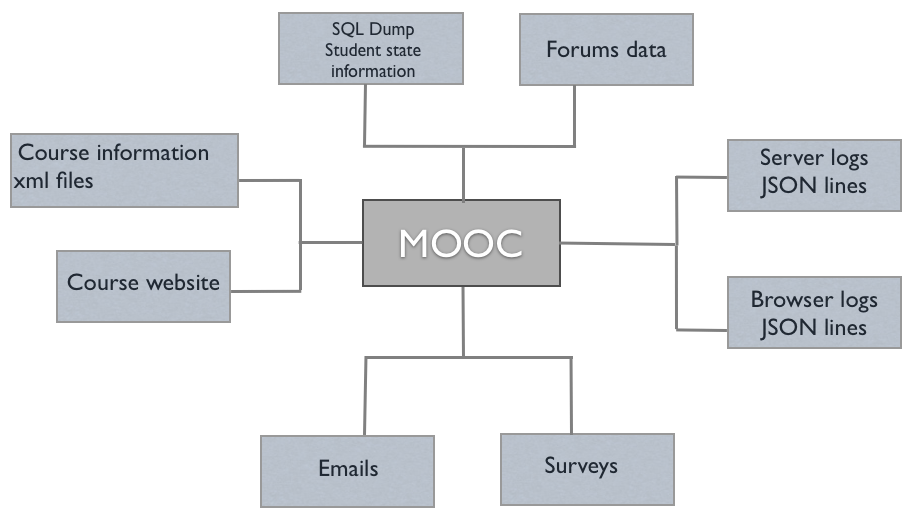
\includegraphics[width=1.0\textwidth]{figures/data_layout.png}
\end{figure}

Figure \ref{fig:data_layout} summarizes the raw data received.

This data included:
\begin{itemize}
\item 154,763 registered students
\item 17.8 million submission events
\item 132.3 million navigational events \footnote{We received more navigational events, but only 132.3 million were well formed enough to be reliably considered for this thesis. }
\item $\sim$90,000 forum posts
\end{itemize}

To analyze this data at scale, as well as write reusable analysis scripts, we first organized the data into a schema designed to capture pertinent information. The resulting database schema, MOOCdb, is designed to capture MOOC data across platforms thereby promoting collaboration among MOOC researchers. MOOCdb utilizes a large series of  scripts to pipe the 6.002x raw data into a standardized schema. More about MOOCdb can be found in the MOOCdb Tech report, but the details are outside the scope of this thesis \cite{tr}.

Through the labor intensive process of piping the raw data into a schematized database, we were able to significantly reduce the data size in terms of disk space. The original $\sim$70GB of raw data was reduced to a $\sim$7GB MOOCdb through schema normalization. The transformation was crucial in order to load the entire database into RAM enabling prompt queries and feature extractions. Figure~\ref{fig:data_reduction} shows a snapshot of the original JSON transactional data transformed into a normalized schema.

\begin{figure}[ht!]
  \caption{Piping data into MOOCdb}\label{fig:data_reduction}
  \centering
    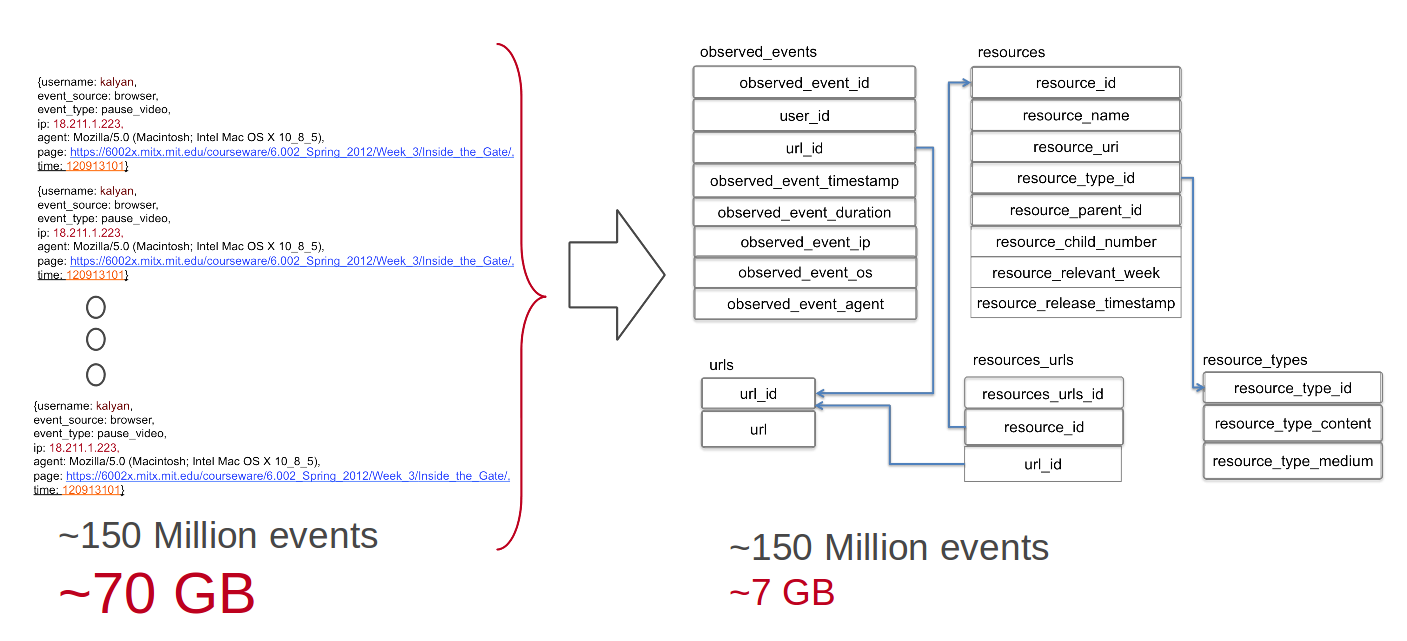
\includegraphics[width=1.0\textwidth]{figures/data_reduction.png}
\end{figure}

\section{Prediction problem assumptions}
We made several assumptions to more precisely define the \sti prediction problem and interpret the data. These assumptions include time-slice delineation and defining persistence (\sti) as the event we attempt to predict.

\subsection{Time-slice delineation}
Temporal prediction of a future event requires us to assemble explanatory variables along a time axis. This axis is subdivided to express the time-varying behavior of variables so they can be used for explanatory purposes. In 6.002x, course content was assigned and due on a weekly basis, where each week corresponded to a module. Owing to the regular modular structure, we decided to define time slices as weekly units. Time slices started the first week in which course content was offered, and ended in the fifteenth week, after the final exam had closed.

\subsection{Stopout definition}
The next question we had to address was our definition of stopout. We considered defining it by the student's last interaction in the course, regardless of the nature of the interaction. This is the approach taken by Balakrishnan in his \sti analysis \cite{balakrishnan2013predicting}. However, Balakrishnan's definition yields noisy results because it gives equal weight to a passive interaction (viewing a lecture, accessing an assignment, viewing a Wiki etc) as it does to a pro-active interaction (submitting a problem, midterm, assignment etc). A student could stop submitting assignments in the course after week 2, but continue to access the course pages and not be considered stopped out. Instead, we define the stop-out point as the time slice (week) a student fails to submit any further assignments or exercise problems. To illustrate, if a student submits his/her last assignment in the third module, he/she is considered to have stopped-out at week four. A submission (or attempt) is a submission of any problem type (Homework, lab, exam etc.), as defined in MOOCdb. This definition narrows the research to students who consistently participate in the course by submitting assignments. Using this definition for \sti we extracted the week number when each student in the cohort stopped out.

Figure~\ref{fig:dropout_week} shows the distribution of \sti week for all 105,622 students who ever accessed the course. Of these, 52,683 students stopped out on week one. These students never submitted an assignment, and are never considered in the rest of our analysis. Another large student drop off point is in week 15, the last week of the course. Many of these students actually finished the course, but did so by submitting their final exam in week 14. This nuance presented itself because students had a range of time to start the final exam, and this range actually overlapped between weeks 14 and 15. Due to the nature of the final exam time range, we never attempt to predict week 15, and consider week 14 as the final week.

\begin{figure}[ht!]
  \caption{Stopout week distribution}\label{fig:dropout_week}
  \centering
    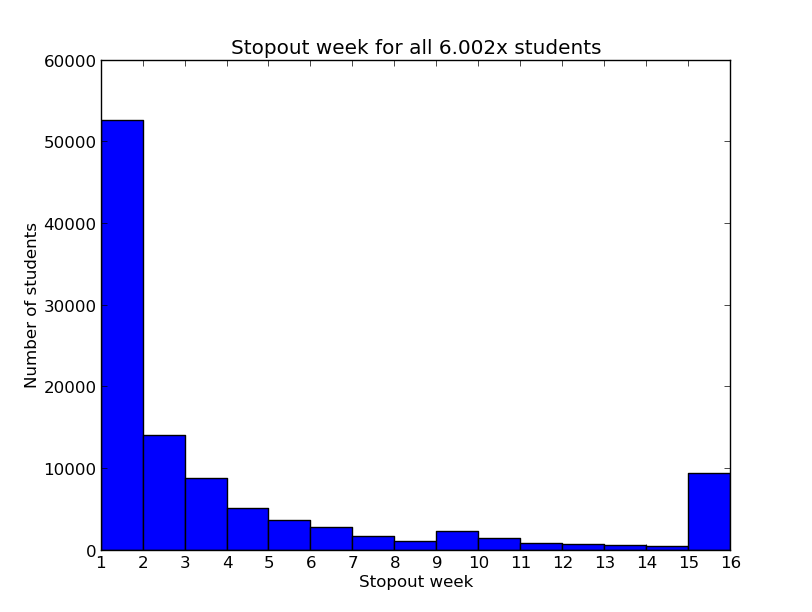
\includegraphics[width=1.0\textwidth]{figures/dropout_weeks.png}
\end{figure}

\subsection{Lead and Lag}
Lead represents how many weeks in advance to predict \sti. We assign the \sti label (\x{1}, 0 for \sti or 1 for persisted) of the lead week as the predictive problem label. Lag represents how many weeks of historical variables will be used to classify. For example, if we use a lead of 5 and a lag of 3, we would take the first 3 weeks of data to predict 5 weeks ahead. Thus, each training data point is a student's feature values for weeks 1, 2 and 3 as features. The binary \sti value for week 8 becomes the label. Figure \ref{fig:lead_lag} shows a diagram of this scenario.

\begin{figure}[!ht]
  \caption{Diagram of the students' weeks data used in a lead 5, lag 3 prediction problem}\label{fig:lead_lag}
  \centering
    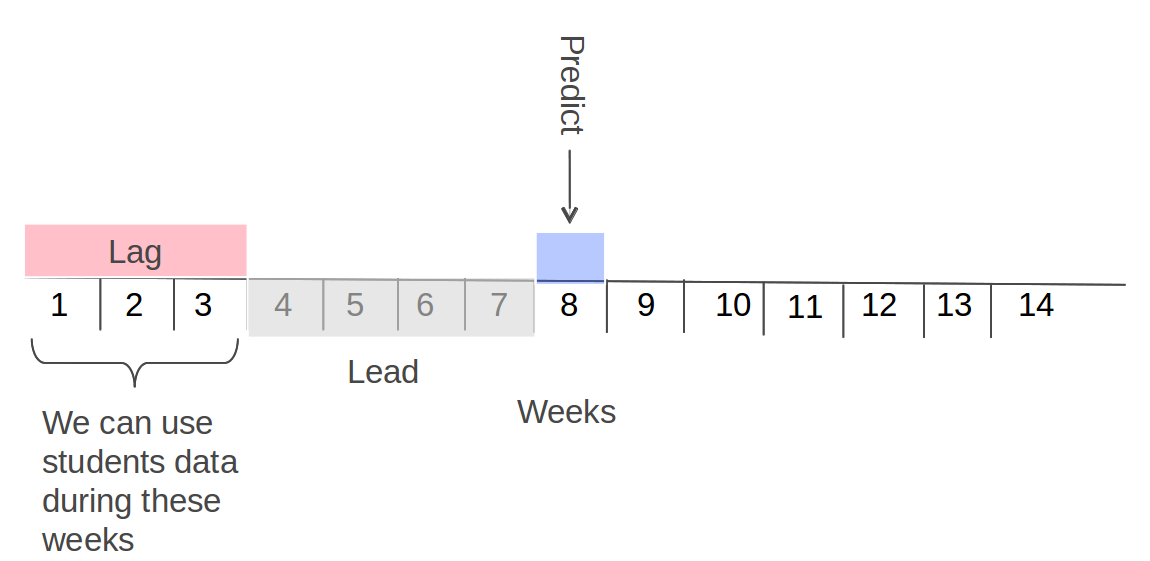
\includegraphics[width=1.0\textwidth]{figures/lead_lag.png}
\end{figure}

We are careful not to use students' stopped out week's features as input to our models. In other words, if a student has stopped out in week 1, 2 or 3, we do not use this student as a data point. Including stopped out student data makes the classification problem too easy as the model will learn that a stopped out student never returns (by our \sti definition).

\section{Dataset partitioning into cohorts}
Rather than treat all students uniformly, we decided to build predictive models for different types of students. With this in mind we divided the students into cohorts as a rough surrogate variable for their commitment to the course. We chose four cohorts based on the student’s collaborative activity throughout the course. More specifically, we divided students based on whether or not they participated in the class forum or helped edit the class Wiki pages. The four types of students are:

\begin{itemize}
\item \neither - these students never actively participated in either the forum or the Wiki. They are named passive because they passively viewed, but did not contribute to, resources.
\item \wiki - these students actively participated in the Wiki by generating Wiki content through their edits, but never actively posted in the forum.
\item \forum - these students actively posted in the forum, but never actively participated in the class Wiki.
\item \both - these students actively participated by generating Wiki content and by posting in the forum
\end{itemize}

From the combined dataset of 52,939 participating students, we assigned each student into one of the four types. The following chart summarizes the sizes of the cohort datasets.

\begin{figure}[!ht]
  \caption{Chart of the relative sizes of our cohorts}\label{fig:cohort_split}
  \centering
    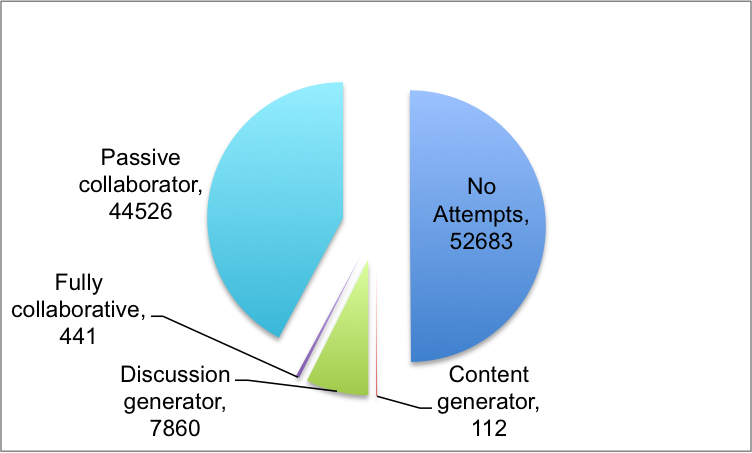
\includegraphics[width=1.0\textwidth]{figures/cohort_split.png}
\end{figure}

For all of the ensuing modelling and analysis, we treated and reported on each of the cohort datasets independently.

\chapter{Constructing Interpretive Features}\label{chap:features}

After collecting the data and carefully defining the problem, we started constructing sophisticated interpretive features (aka \cov) hypothesized to be predictive of \sti. As previously mentioned, we split the course into 15 time slices (weeks). Thus, for each defined feature, we assign each student a feature-value each week. For example, each student has a value for the feature ‘\sti’ for each of the 15 weeks. The value is 0 if the student has already stopped out by not submitting any more assignments, or it is 1 if the student will submit assignments in the future.

\section{Feature origins}

With the database, we then proceeded to write the scripts to extract the \cov for our model. By analyzing the \cov we aimed to capture behavioral patterns that could be indicative of loss of interest or loss of motivation among several others. We approached this in three different ways:

\begin{itemize}
\item We brainstormed feature ideas as researchers. Next, we implemented our own ideas by writing feature extraction scripts. We call these features \selfself.
\item We asked others for ideas of what might be predictive of \sti. The people we asked included students, teachers and external researchers. We refer to this group collectively as `the crowd.' We identified ideas that we had not implemented yet, and constructed feature extraction scripts ourselves. We call these \crowdself.
\item Finally, we asked `the crowd' to brainstorm predictive features, and to send us feature extraction scripts that we could run on MOOCdb. We provided people with a mock dataset with an identical data schema. Thus, instead of providing actual student data, we empowered the crowd to join in our data science efforts. We call the resulting features \crowdcrowd.
\end{itemize}


\subsection{\selfself}
Table \ref{table:self_proposed_self_extracted} summarizes the features we brainstormed and extracted. Each feature is calculated on a per student, per week basis. A * indicates that a disambiguating explanation follows underneath.

\begin{table*}[htp]
	\centering
	\caption{List of \selfself \cov}\label{table:self_proposed_self_extracted}
{
		\begin{tabular}{|c|p{4cm}|p{10cm}|}
			\hline
							& Name 													& Definition																									 \\ \hline
			\x{1}		& stopout 											& Whether the student has stopped out or not 									\\ \hline
			*\x{2}	& total duration								& Total time spent on all resources														\\ \hline
			\x{3}		& number forum posts						& Number of forum posts																				\\ \hline
			\x{4}		& number wiki edits							& Number of wiki edits																				\\ \hline
			*\x{5}	& average length forum post			& Average length of forum posts																\\ \hline 
			*\x{6}		& number distinct problems submitted	& Number of distinct problems attempted 							\\ \hline 
			*\x{7}	& number submissions						& Number of submissions \footnote{In our terminology, a submission corresponds to a problem attempt. In 6.002x, students could submit multiple times to a single problem. We therefore differentiate between problems and submissions.}																				\\ \hline
			\x{8}		& number distinct problems correct & Number of distinct correct problems 											\\ \hline 
			\x{9}	& average number submissions					& Average number of submissions per problem (\x{7} / \x{6})			\\ \hline 
			\x{10} & observed event duration per correct problem		& Ratio of total time spent to number of distinct correct problems (\x{2} / \x{8}). This is the inverse of the percent of problems correct \\ \hline 
			\x{11} & submissions per correct problem		& Ratio of number of problems attempted to number of distinct correct problems	(\x{6} / \x{8})	\\ \hline
			\x{12} & average time to solve problem	& Average time between first and last problem submissions for each problem (average(max(submission.timestamp) - min(submission.timestamp) for each problem in a week) )															\\ \hline
			*\x{13} & observed event variance			& Variance of a student's observed event timestamps  					 \\ \hline
			\x{14} & number collaborations				& Total number of collaborations	(\x{3} + \x{4})														 \\ \hline
			\x{15} & max observed event duration	& Duration of longest observed event													 \\ \hline
			*\x{16} & total lecture duration				& Total time spent on lecture resources 											\\ \hline
			*\x{17} & total book duration					& Total time spent on book resources													 \\ \hline
			*\x{18} & total wiki duration					& Total time spent on wiki resources													 \\ \hline
		\end{tabular}
	}
\end{table*}

\begin{itemize}

\item \x{2}, \x{16}, \x{17}, \x{18}: These features are based on observed event duration. The edX server logs did not explicitly provide this, so we need to infer the duration based on the timestamps of the start of observed events. We assume that a student observed an event until he observed a different event (a new timestamp). This is a similar approach used by industry web-profile metrics. Sometimes, the spacing between observed events is very large, presumably because the user stopped interacting with the website. This is handled by setting the last observed event's duration to a MAX\_DURATION. For example, if Student A had three observed events with timestamps, T1, T2 and T3, the duration of the first event would be T2 - T1, the duration of the second is T3 - T2, and the duration of the third is MAX\_DURATION, since there is no T4. Additionally if $T3 - T2 > 60$, the duration is set to MAX\_DURATION. In our case, we set MAX\_DURATION to be 60 minutes, because our data included durations of up to $\sim$ 60 minutes.

\item \x5: A forum post's length is the number of characters in the forum post (i.e. the length of the string). We used MySQL's length function.

\item \x6, \x7: With problem submissions, week number is ambiguous. Students may submit a problem at any time (assuming the problem is released), regardless of when the problem is due. In other words, even if a problem corresponds to week number 3, a student could submit that problem in week 5. For these features, we counted a submission in week w1 if the submission's timestamp is in w1, regardless of whether or not the problem is part of w1's assigned content.  We chose to do this because the feature is meant to capture a student's weekly activity.

\item \x{13}: For this feature, we tried to measure the consistency of a student's observed event patterns relative to the time of day (i.e., a student who always works on the course at 7:00 a.m. would have small variance for that week). To capture event variance, for each day, we counted the number of seconds after midnight of the observed event timestamp. We created a distribution of all of the number of seconds for each student each week. Then, we calculated the variance of the distribution (each student, week pair has it's own distribution). This variance becomes the feature. Note: student's participate from around the world, but the timestamp is in UTC time. However, because variance is valued over absolute value, the actual time is irrelevant. 

\end{itemize}

\subsection{\crowdself}\label{section:crowdself}
Table \ref{table:crowd_proposed_self_extracted} summarizes the features the crowd hypothesized, but we extracted. Each feature is calculated on a per student, per week basis. A * indicates that a disambiguating explanation follows underneath.

\begin{table*}[htp]
	\centering
	\caption{List of \crowdself \cov}\label{table:crowd_proposed_self_extracted}
{
		\begin{tabular}{|c|p{4cm}|p{10cm}|}
			\hline
							& Name 													& Definition																									 \\ \hline
			$x_{201}$ & number forum responses			& Number of forum responses																		\\ \hline
			*$x_{202}$ & average number of submissions percentile	& A student's average number of submissions (feature 9) as compared with other students that week as a percentile				\\ \hline
			*$x_{203}$ & average number of submissions percent	& A student's average number of submissions (feature 9) as a percent of the maximum average number of submissions that week																																			\\ \hline
			*$x_{204}$ & pset grade										& Number of the week's homework problems answered correctly / number of that week's homework problems																																												\\ \hline
			$x_{205}$ & pset grade over time					& Difference in grade between current pset grade and average of student's past pset grade																																																					\\ \hline
			*$x_{206}$ & lab grade										& Number of the week's lab problems answered correctly / number of that week's lab  problems																																																\\ \hline
			$x_{207}$ & lab grade over time						& Difference in grade between current lab grade and average of student's past lab grade																																																					\\ \hline
			$x_{208}$ & number submissions correct		& Number of correct submissions																\\ \hline
			$x_{209}$ & correct submissions percent		& Percentage of the total submissions that were correct ($x_{208}$ / $x_{7}$)													\\ \hline
			*$x_{210}$ & average predeadline submission time & Average time between a problem submission and problem due date over each submission that week																																									\\ \hline
		\end{tabular}
	}
\end{table*}

\begin{itemize}

\item \x{202}, \x{203}: For each week, we create a distribution of all of the values for every student of feature \x9. Then, we compare a student's \x9 value to the distribution for that week. \x{202} is the percentile over that distribution, and \x{203} is the percent as compared to the max of the distribution.

\item \x{204}, \x{206}: As mentioned earlier, with regard to submissions, there is an ambiguity: whether a submission correspond to the week in which it was submitted, or the week in which the problem's module was. These features are meant to capture the grade on the module. Therefore, they are computed based on the week's homework assignment and lab assignment, rather than on the submission timestamp. The number of problems the student answered correctly out of the total number of homework or lab problems corresponding to that week constitute features \x{204} and \x{206}.

\item \x{210}: For each submission during the week, the time difference between the submission timestamp and the due date of the problem is calculated. \x{210} is the average of all of these differences. 

\end{itemize}

\subsection{\crowdcrowd}

In an attempt to crowdsource feature extraction, we asked SQL-fluent MIT students and researchers to both hypothesize new features and submit scripts which would extract them. We are still in the process of collecting feature scripts from this effort at the time of writing. Unfortunately, due to an empty field in MOOCdb, we were unable to extract and use several features we have already received. We plan to continue this effort in the future.

\section{Complexity of extracted features}
Efforts have been made by others to construct features to describe student behavior in MOOCs. For example, Balakrishnan constructed 5 basic features, two of which, \sti and the number of forum posts (\x{1} and \x{3}), we independently used \cite{balakrishnan2013predicting}. Those 5 features are basic in the fact that they rely solely on one of the data sources received from MOOC platforms, and only count the number of times an event occurs. However, our extraction effort is the first instance, to our knowledge, that an extensive, sophisticated feature-set has been constructed on MOOC behavioral data. Firstly, our 28 features are more sophisticated in the variety of sources used in their construction, such as the leveraged crowd-sourced brainstorming used to capture creative behavioral features. In addition, many involve complexities beyond a simple count per week. Such complexities include:
\begin{itemize}
\item Higher level statistical features. For example, the variance of the times of day that a student accesses course material each week (\x{13}) and the percentile of a student’s average number of submissions (\x{202}) use statistical metrics about a student’s behavior.
\item Manual curation of features. Some features require manual curation in order to get a descriptive metric. For example, \x{204}, a student’s pset grade, necessitated manual curation of problem and assignment deadlines.
\item Multiple data sources and MOOCdb modes. Some features included information from multiple sources (such as \x{204}, the pset grade). This included getting deadlines for the problems from the XML file, all submissions from the server logs, and the problem’s correctness from the production MySQL dump.
\item Combination features. For example, \x{10} represents the amount of time a student spends on the course (\x{2}) per correct problem (\x{8}). This feature captures the less tangible gratification a student experiences based on time spent.
\end{itemize}

\section{Statistical Analysis}
After constructing MySQL feature extraction scripts to run on MOOCdb \footnote{The software has been prepared to be released with this thesis.}
, we ran each across all students in the 6.002x MOOCdb. This database contained 105,621 students who had some interaction with the class. Running the scripts took several days, as a few of the scripts scanned the entire click-stream observed\_events table for a student, which contains more than 132M entries. 

After extracting our interpretive features, we created a csv dataset with all of the information. This csv file contained the value for all 28 features for 105,621 students across 15 weeks. Each row in the file contained the feature values for specific student\_week, and each column contained the feature values for a specific feature. Thus, we had a (num\_students * num\_weeks) X num\_features or 1,584,315 X 28 csv file.

Although MOOCdb contained 105,621 students, many never participated in submitting problems. Thus, based on our prior definition of stopout, these students had already stopped out by the first week. We removed these students from the dataset. The resulting dataset contained 52,939 students, roughly half of the original. Each of these students participated in submitting problems for at least one week of the course.

\begin{figure}[ht!]
  \caption{The distribution of feature values for \x{2} through \x{10}}\label{fig:features_2_10}
  \centering
    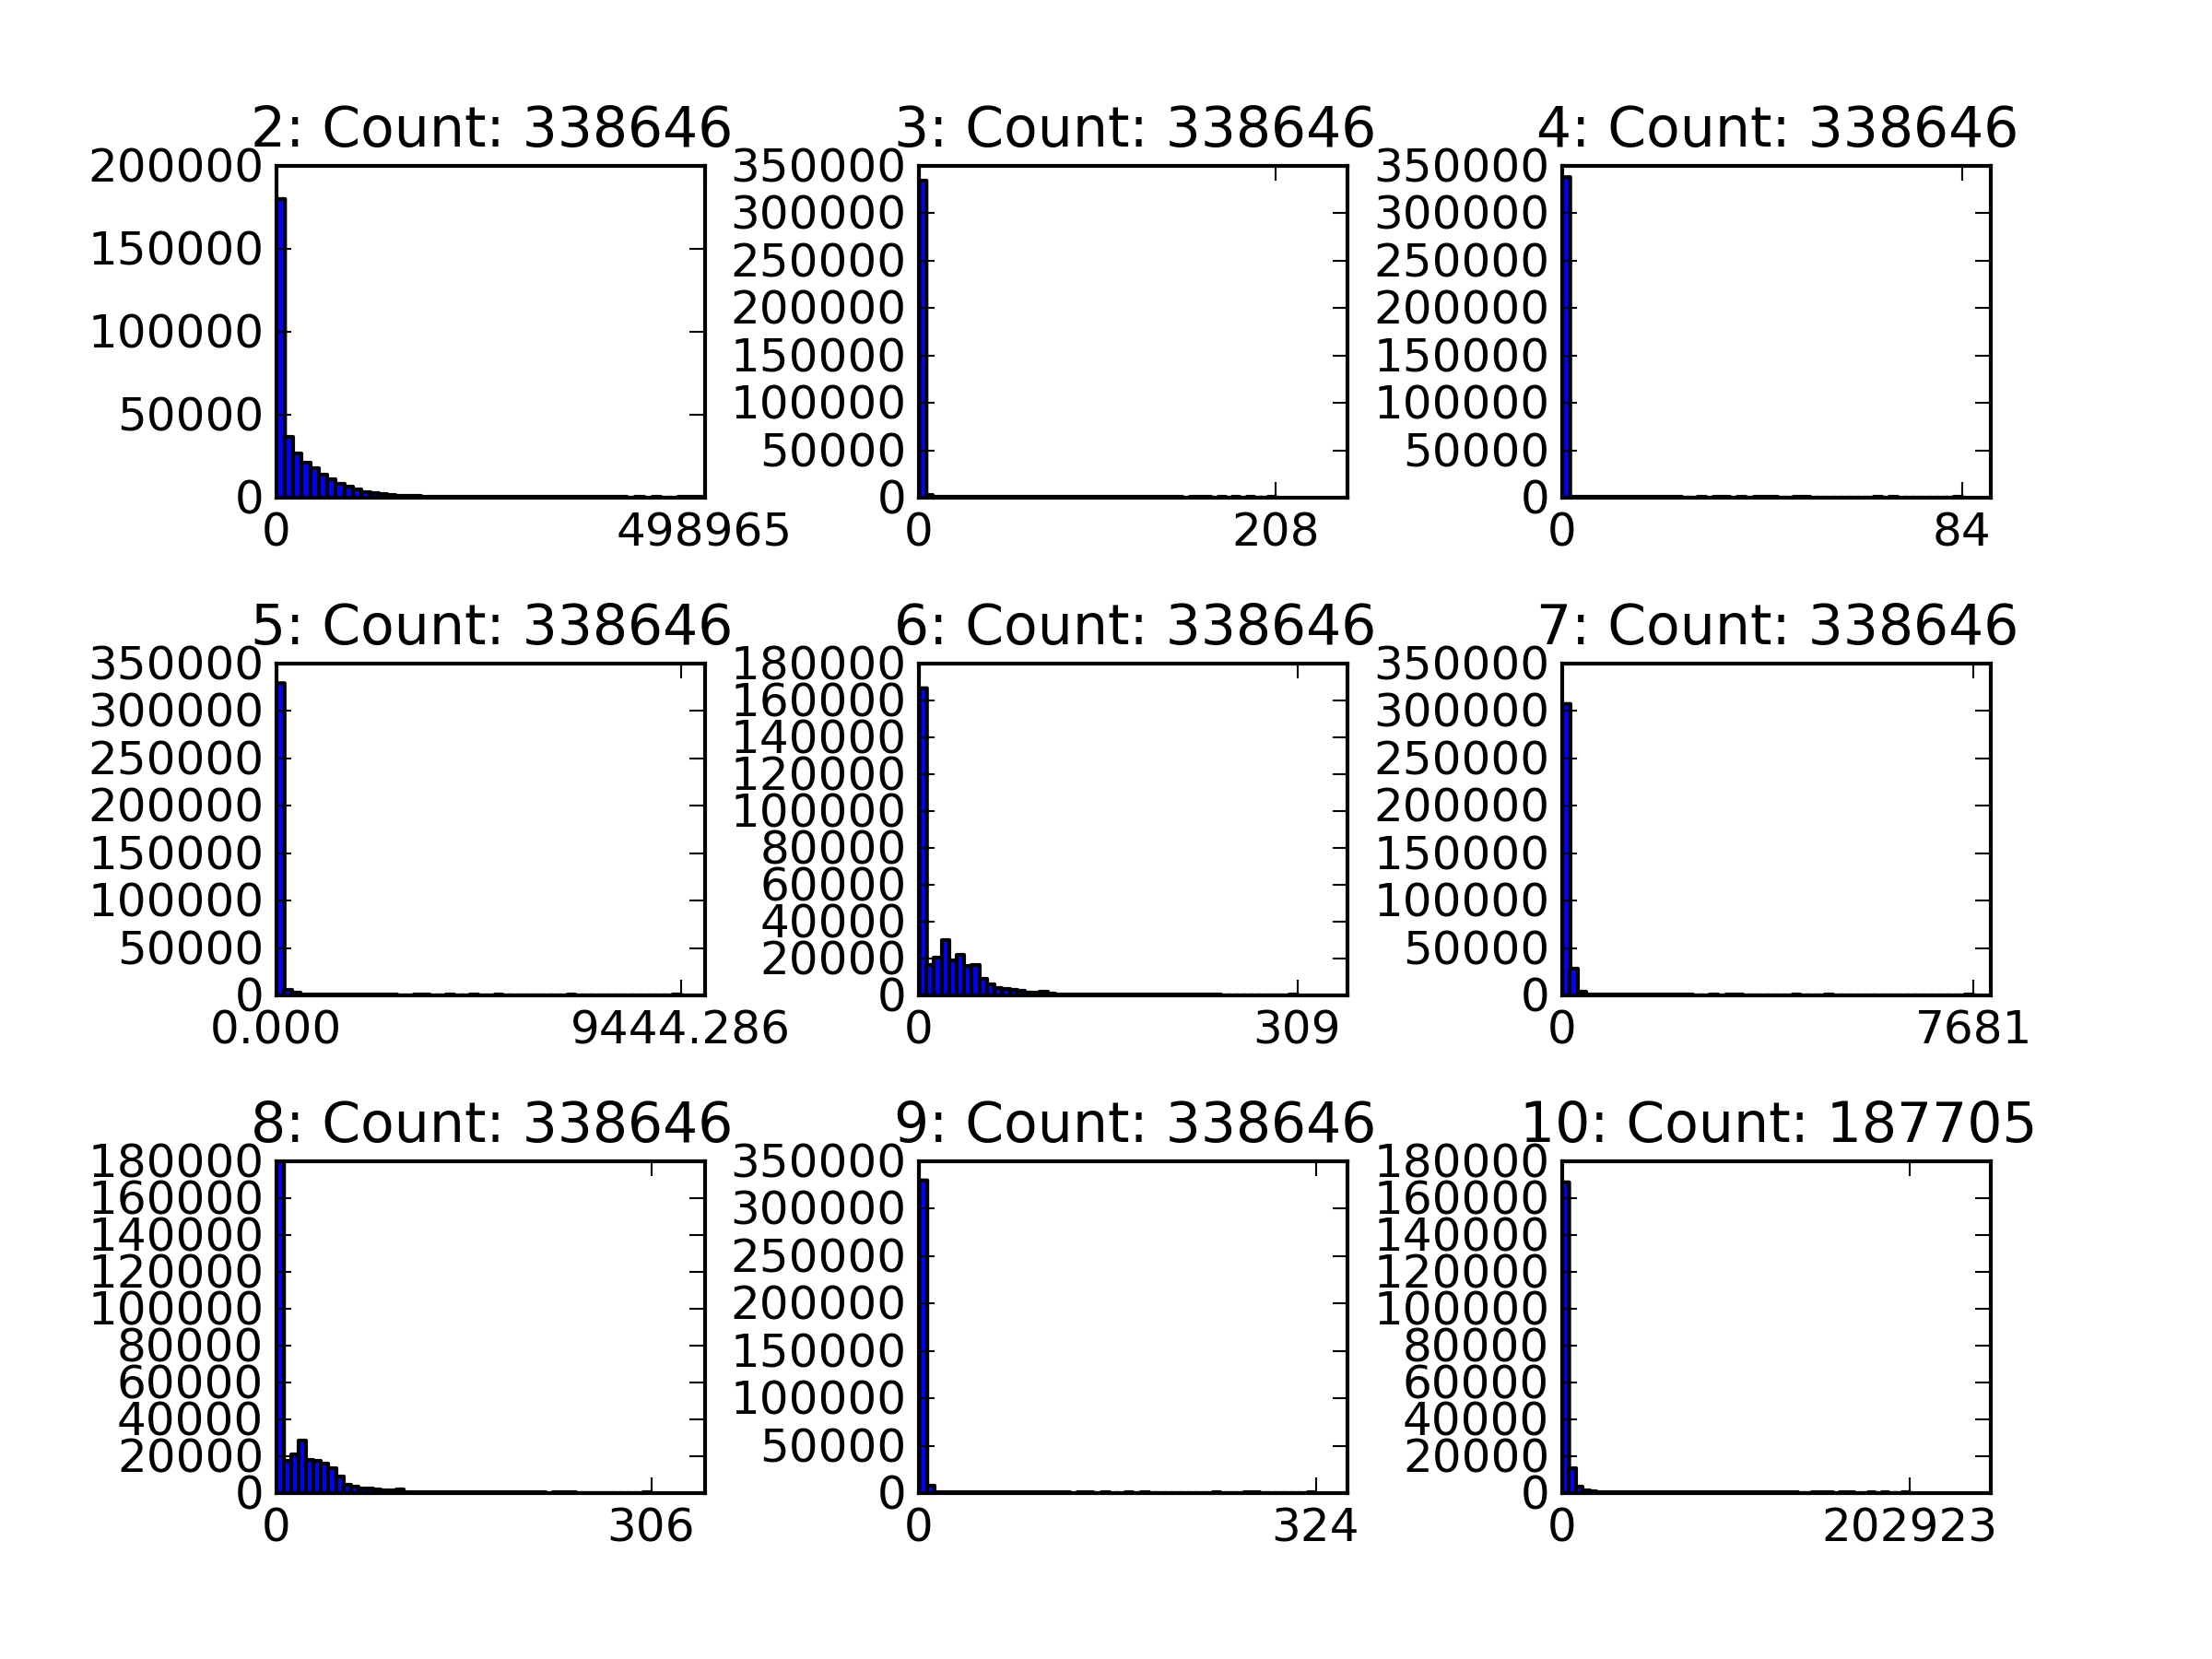
\includegraphics[width=1.0\textwidth]{figures/feature_distributions/features_2_10.png}
\end{figure}

\begin{figure}[ht!]
  \caption{The distribution of feature values for \x{11} through \x{201}}\label{fig:features_11_19}
  \centering
    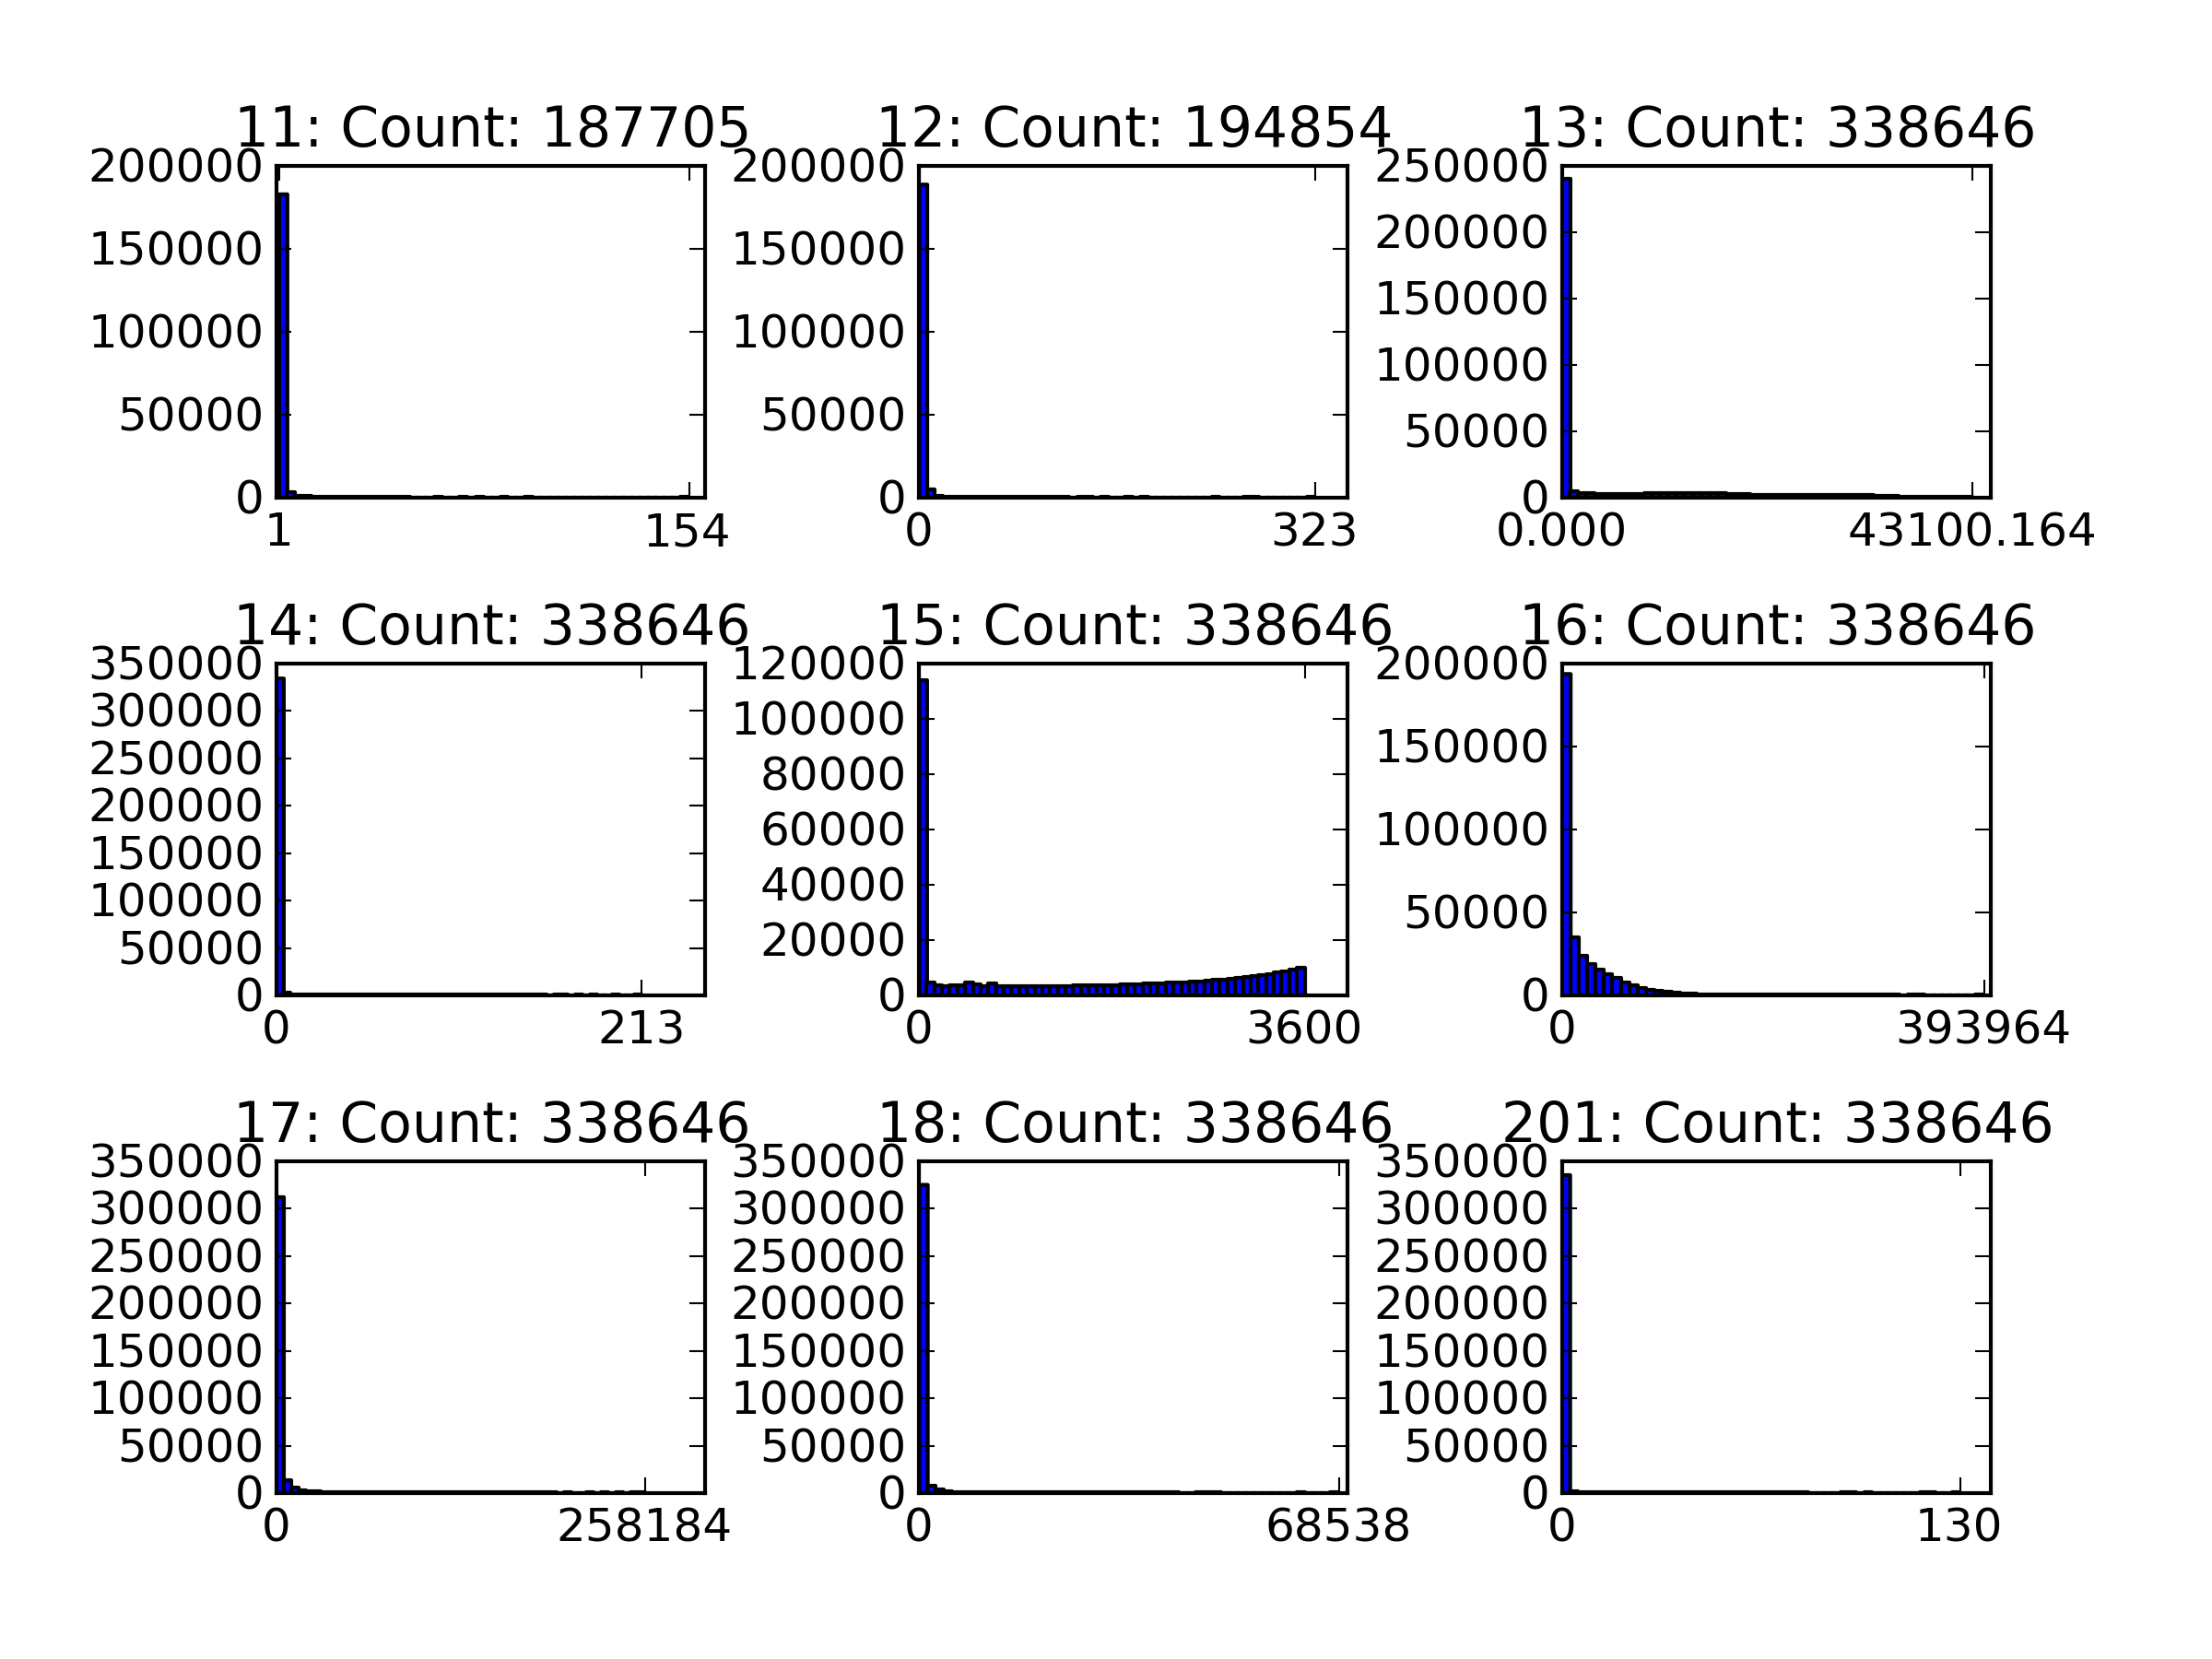
\includegraphics[width=1.0\textwidth]{figures/feature_distributions/features_11_19.png}
\end{figure}

\begin{figure}[ht!]
  \caption{The distribution of feature values for \x{202} through \x{210}}\label{fig:features_20_28}
  \centering
    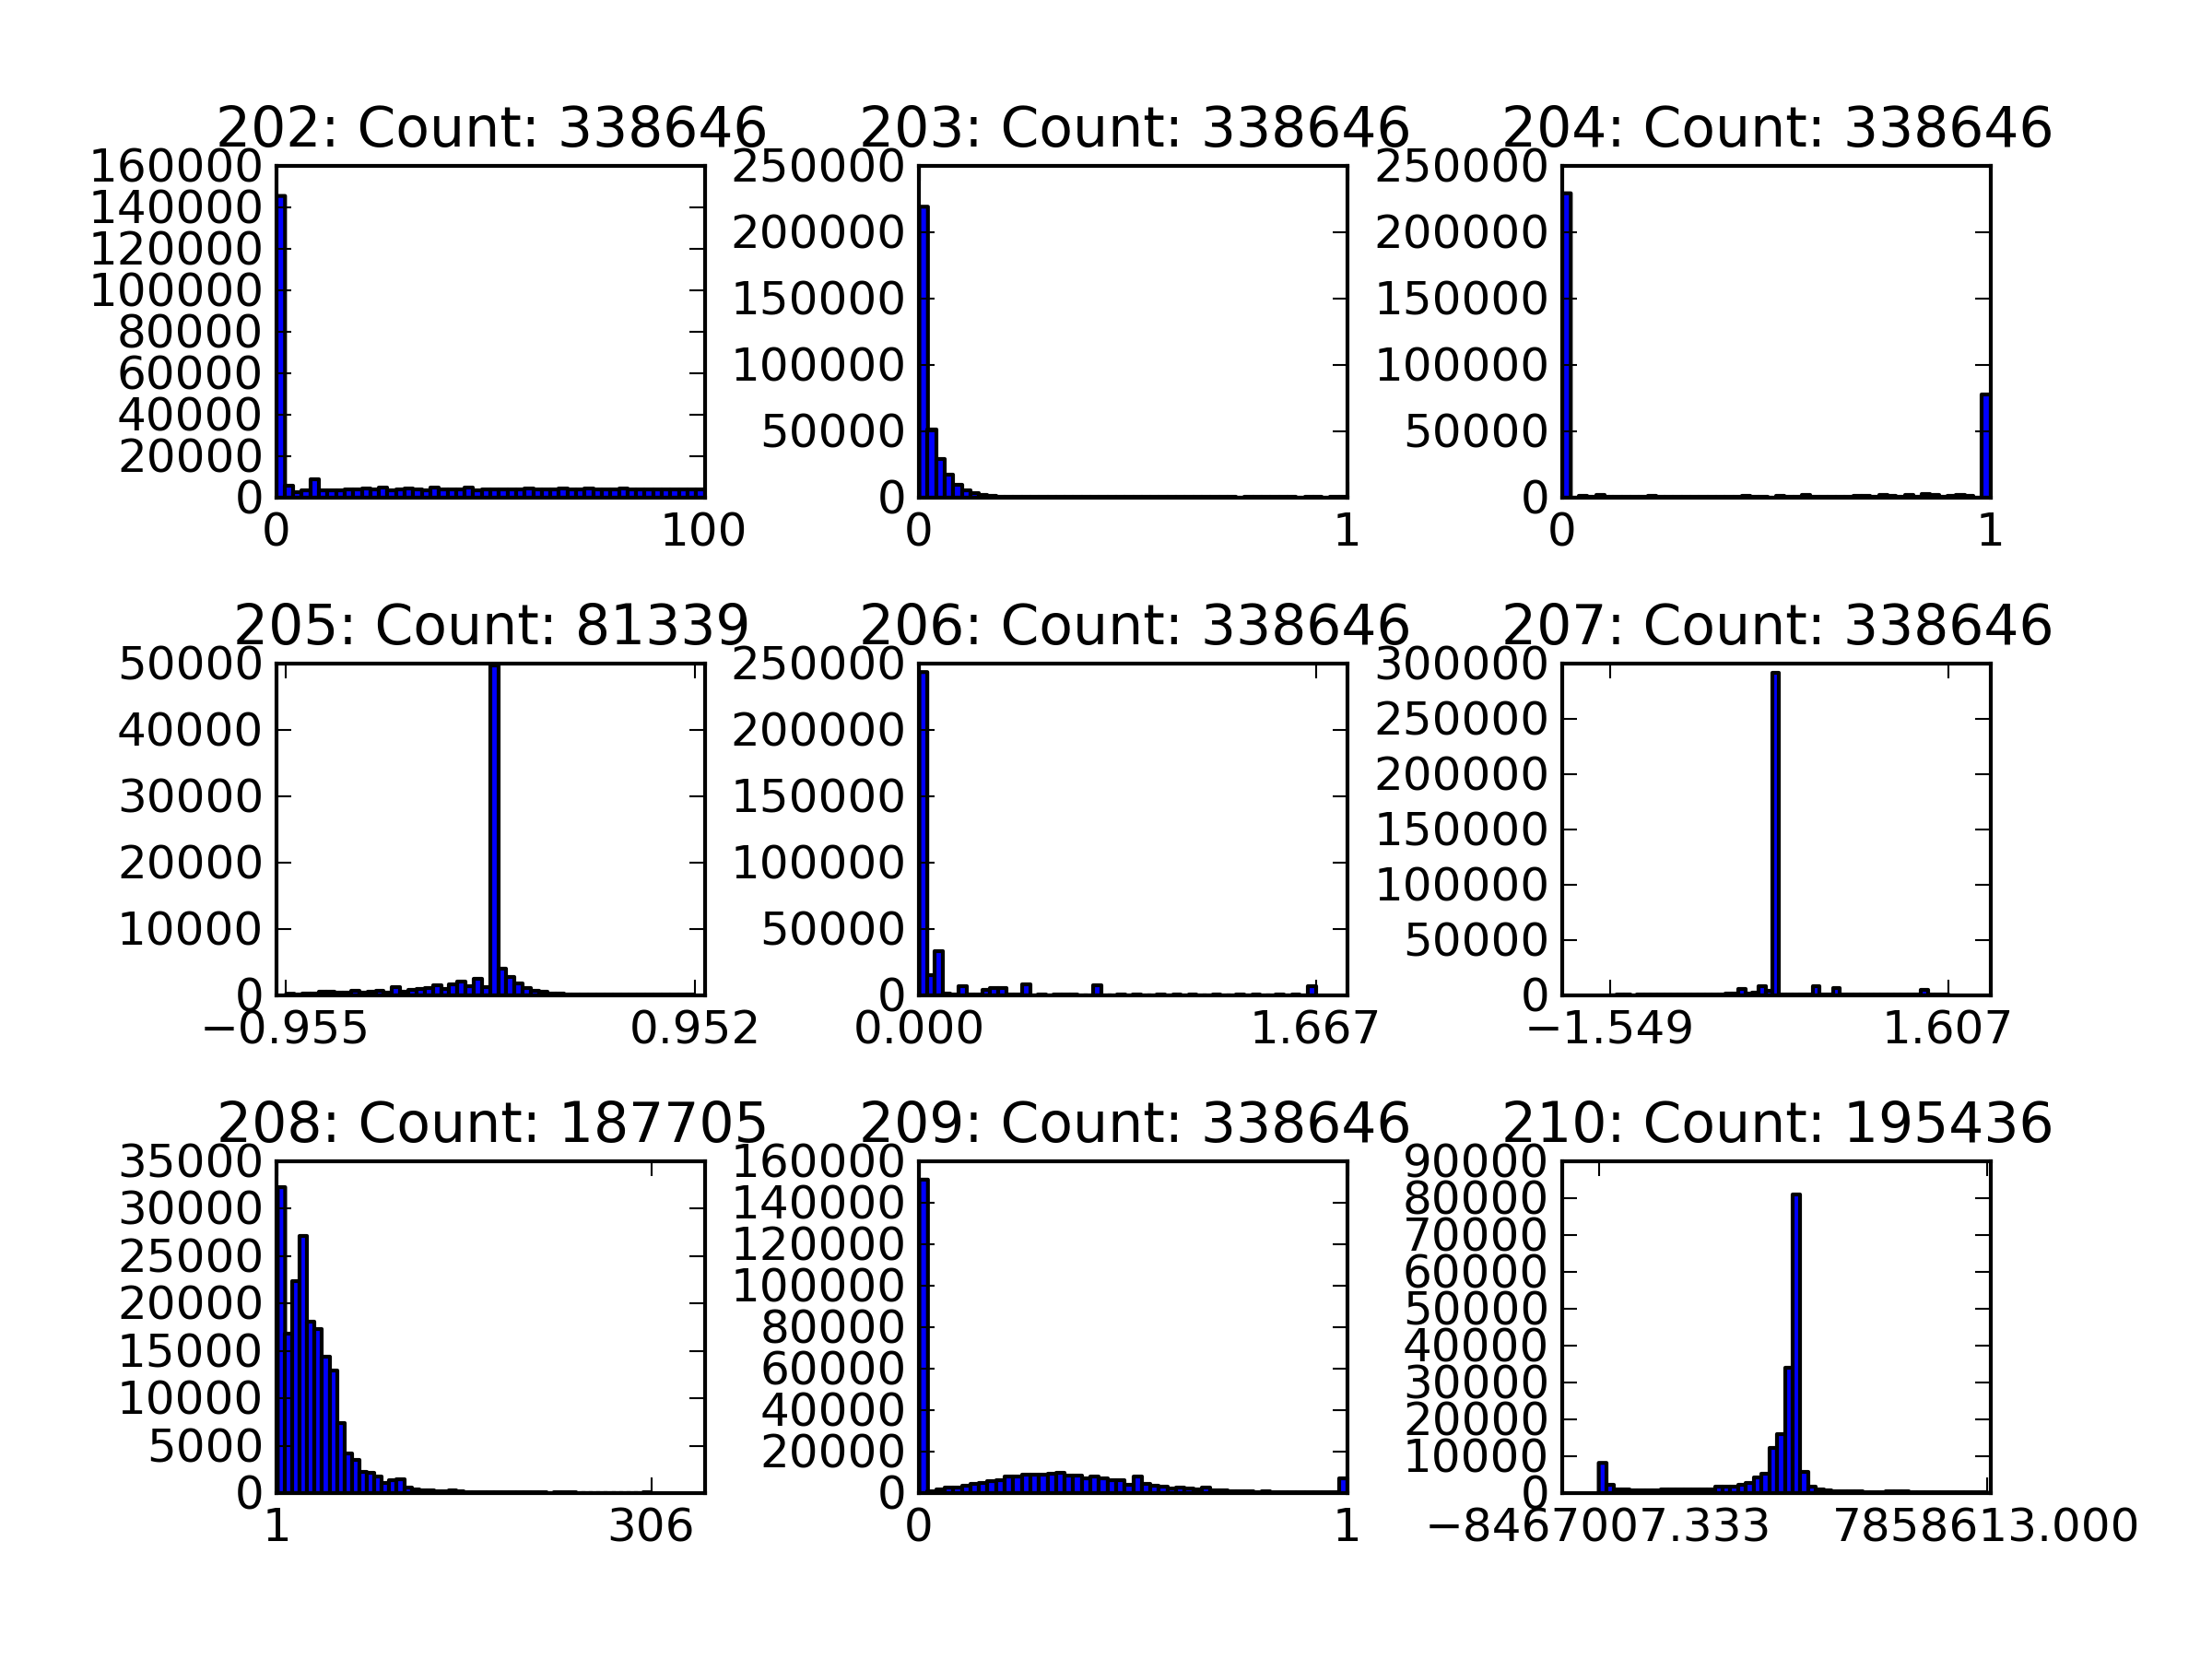
\includegraphics[width=1.0\textwidth]{figures/feature_distributions/features_20_28.png}
\end{figure}

Figures \ref{fig:features_2_10} through \ref{fig:features_20_28} shows the distribution of feature values over every student week where the student was not stopped out. Note that the majority of feature values are 0s. This means there are many weeks where a student did not interact with the course at all, or only interacted with limited course components (for example, never posted on the forum but watched lectures, or only watched lectures but did not submit). Most features are heavily skewed to the right.

\section{Principal Component Analysis}
We performed a dimensionality reduction technique called principal component analysis to transform our extracted features into a basis of lower dimensionality. This technique finds the dimension of the data with the largest variance, and uses this as the first basis dimension. The second basis dimension is the dimension orthogonal to the first which has the largest variance. This process is completed until a full basis is found. The first X dimensions that cover 95\% of the variance are used to transform the features. We use the transformed features as a new dataset. This process not only reduces the dimensionality, but is useful for models that assume feature independence as the PCA features are orthogonal.

Principal component analysis reduced the \neither and \forum cohorts from 28 features to 9 features. PCA transformed the \both cohort into 13 features. We were unable to perform PCA on the \wiki cohort because there were too few students.

\section{Discretization of features}\label{section:binning}
We discretized the extracted feature values as some of our predictive modelling training algorithms rely on discretized values for tractability. This process is also known as ‘binning.’ In order to best discretize a feature, we want to preserve as closely as possibly the distribution of that feature. Inevitably, because we have a smaller range of values than the feature can take, we will lose information when we bin the features, but a good discretization preserves as much information as possible. 
A simple way to bin a continuously valued feature is to use equal sized bins, which works well when the distribution is roughly equally distributed. However, after analyzing our distributions, we realized that our distribution for most features is heavily skewed towards 0. We used a binning strategy that picked binning cutoffs in order to create an equal frequency of samples in each bin. This strategy, as closely as possible, will preserve the original distribution.
We attempted binning with 5 bins and 10 bins. After the binning, we analyzed the distribution of each discretized feature in comparison with the continuous distribution. With just 5 bins, we were able to get almost equal bin frequencies. (see Figures \ref{fig:features_bin_5_2_10} through \ref{fig:features_bin_5_20_28}). Since the distribution roughly captured the entropy, we decided to use 5 bins. Additionally, we knew from prior experiments that a smaller number of bins significantly reduced training and inference times for dynamic Bayesian networks.

\begin{figure}[ht!]
  \caption{The distribution of binned feature values for \x{2} through \x{10}}\label{fig:features_bin_5_2_10}
  \centering
    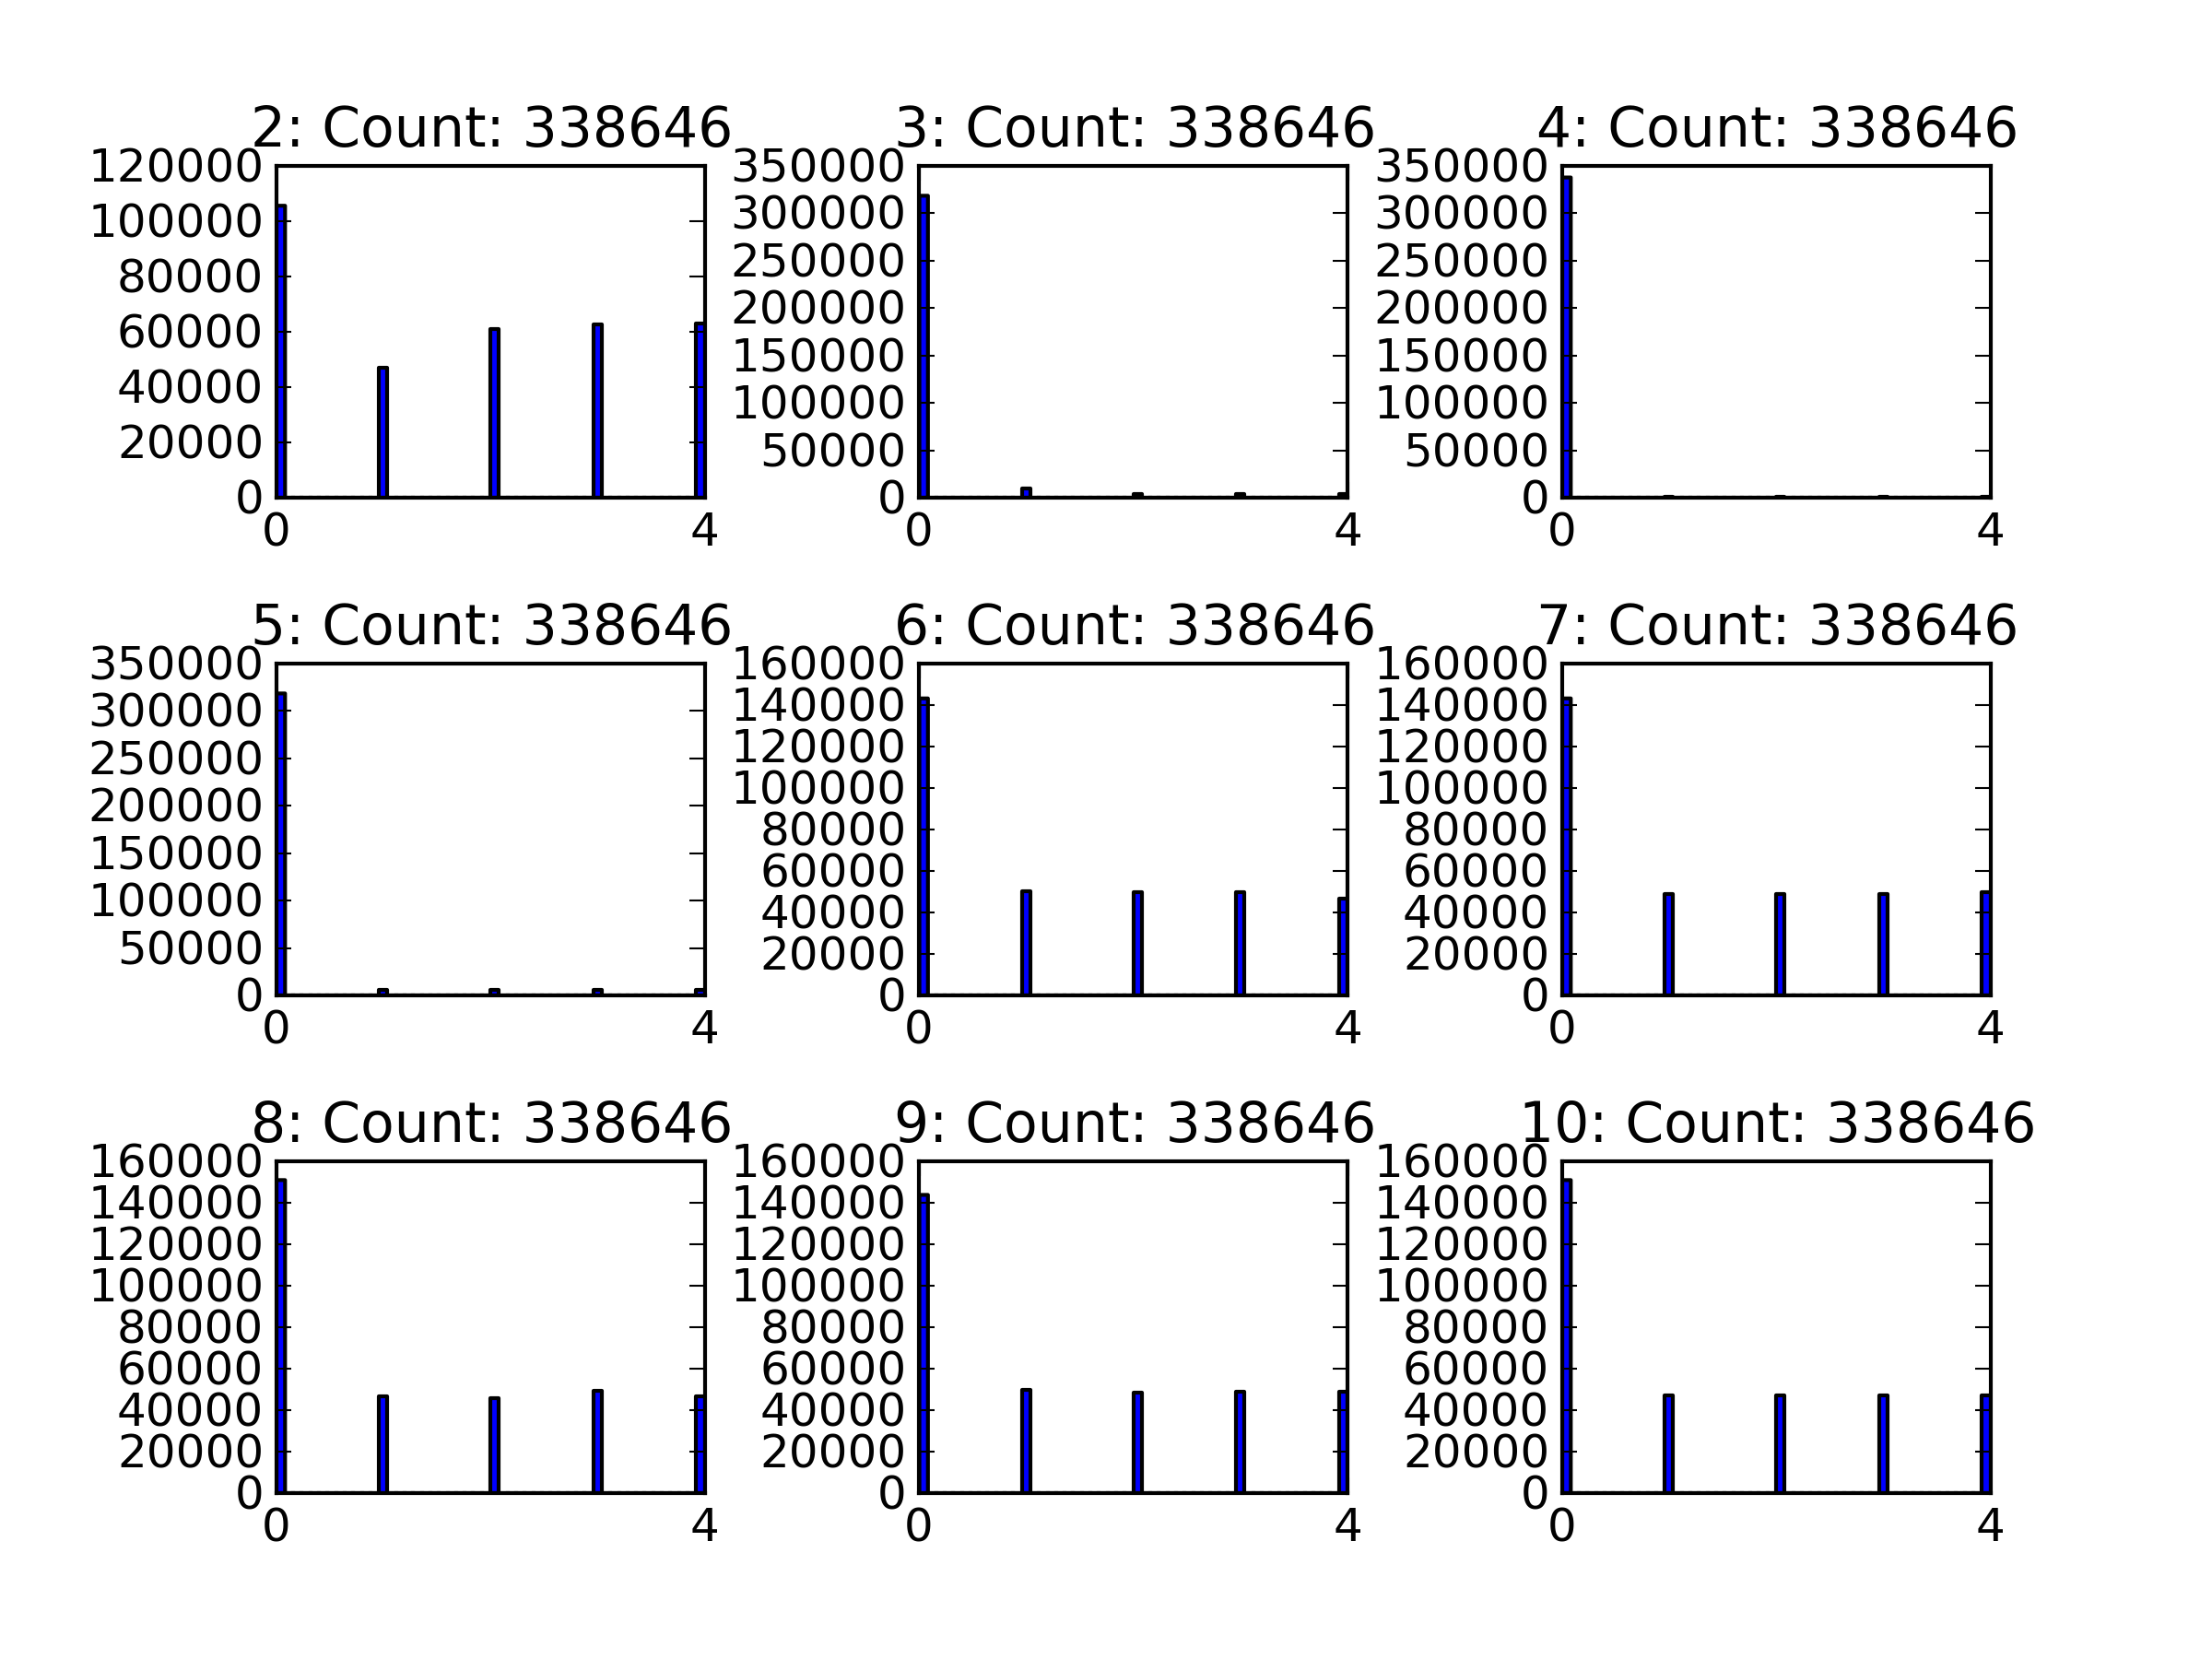
\includegraphics[width=1.0\textwidth]{figures/feature_distributions/features_bin_5_2_10.png}
\end{figure}

\begin{figure}[ht!]
  \caption{The distribution of binned feature values for \x{11} through \x{201}}\label{fig:features_bin_5_11_19}
  \centering
    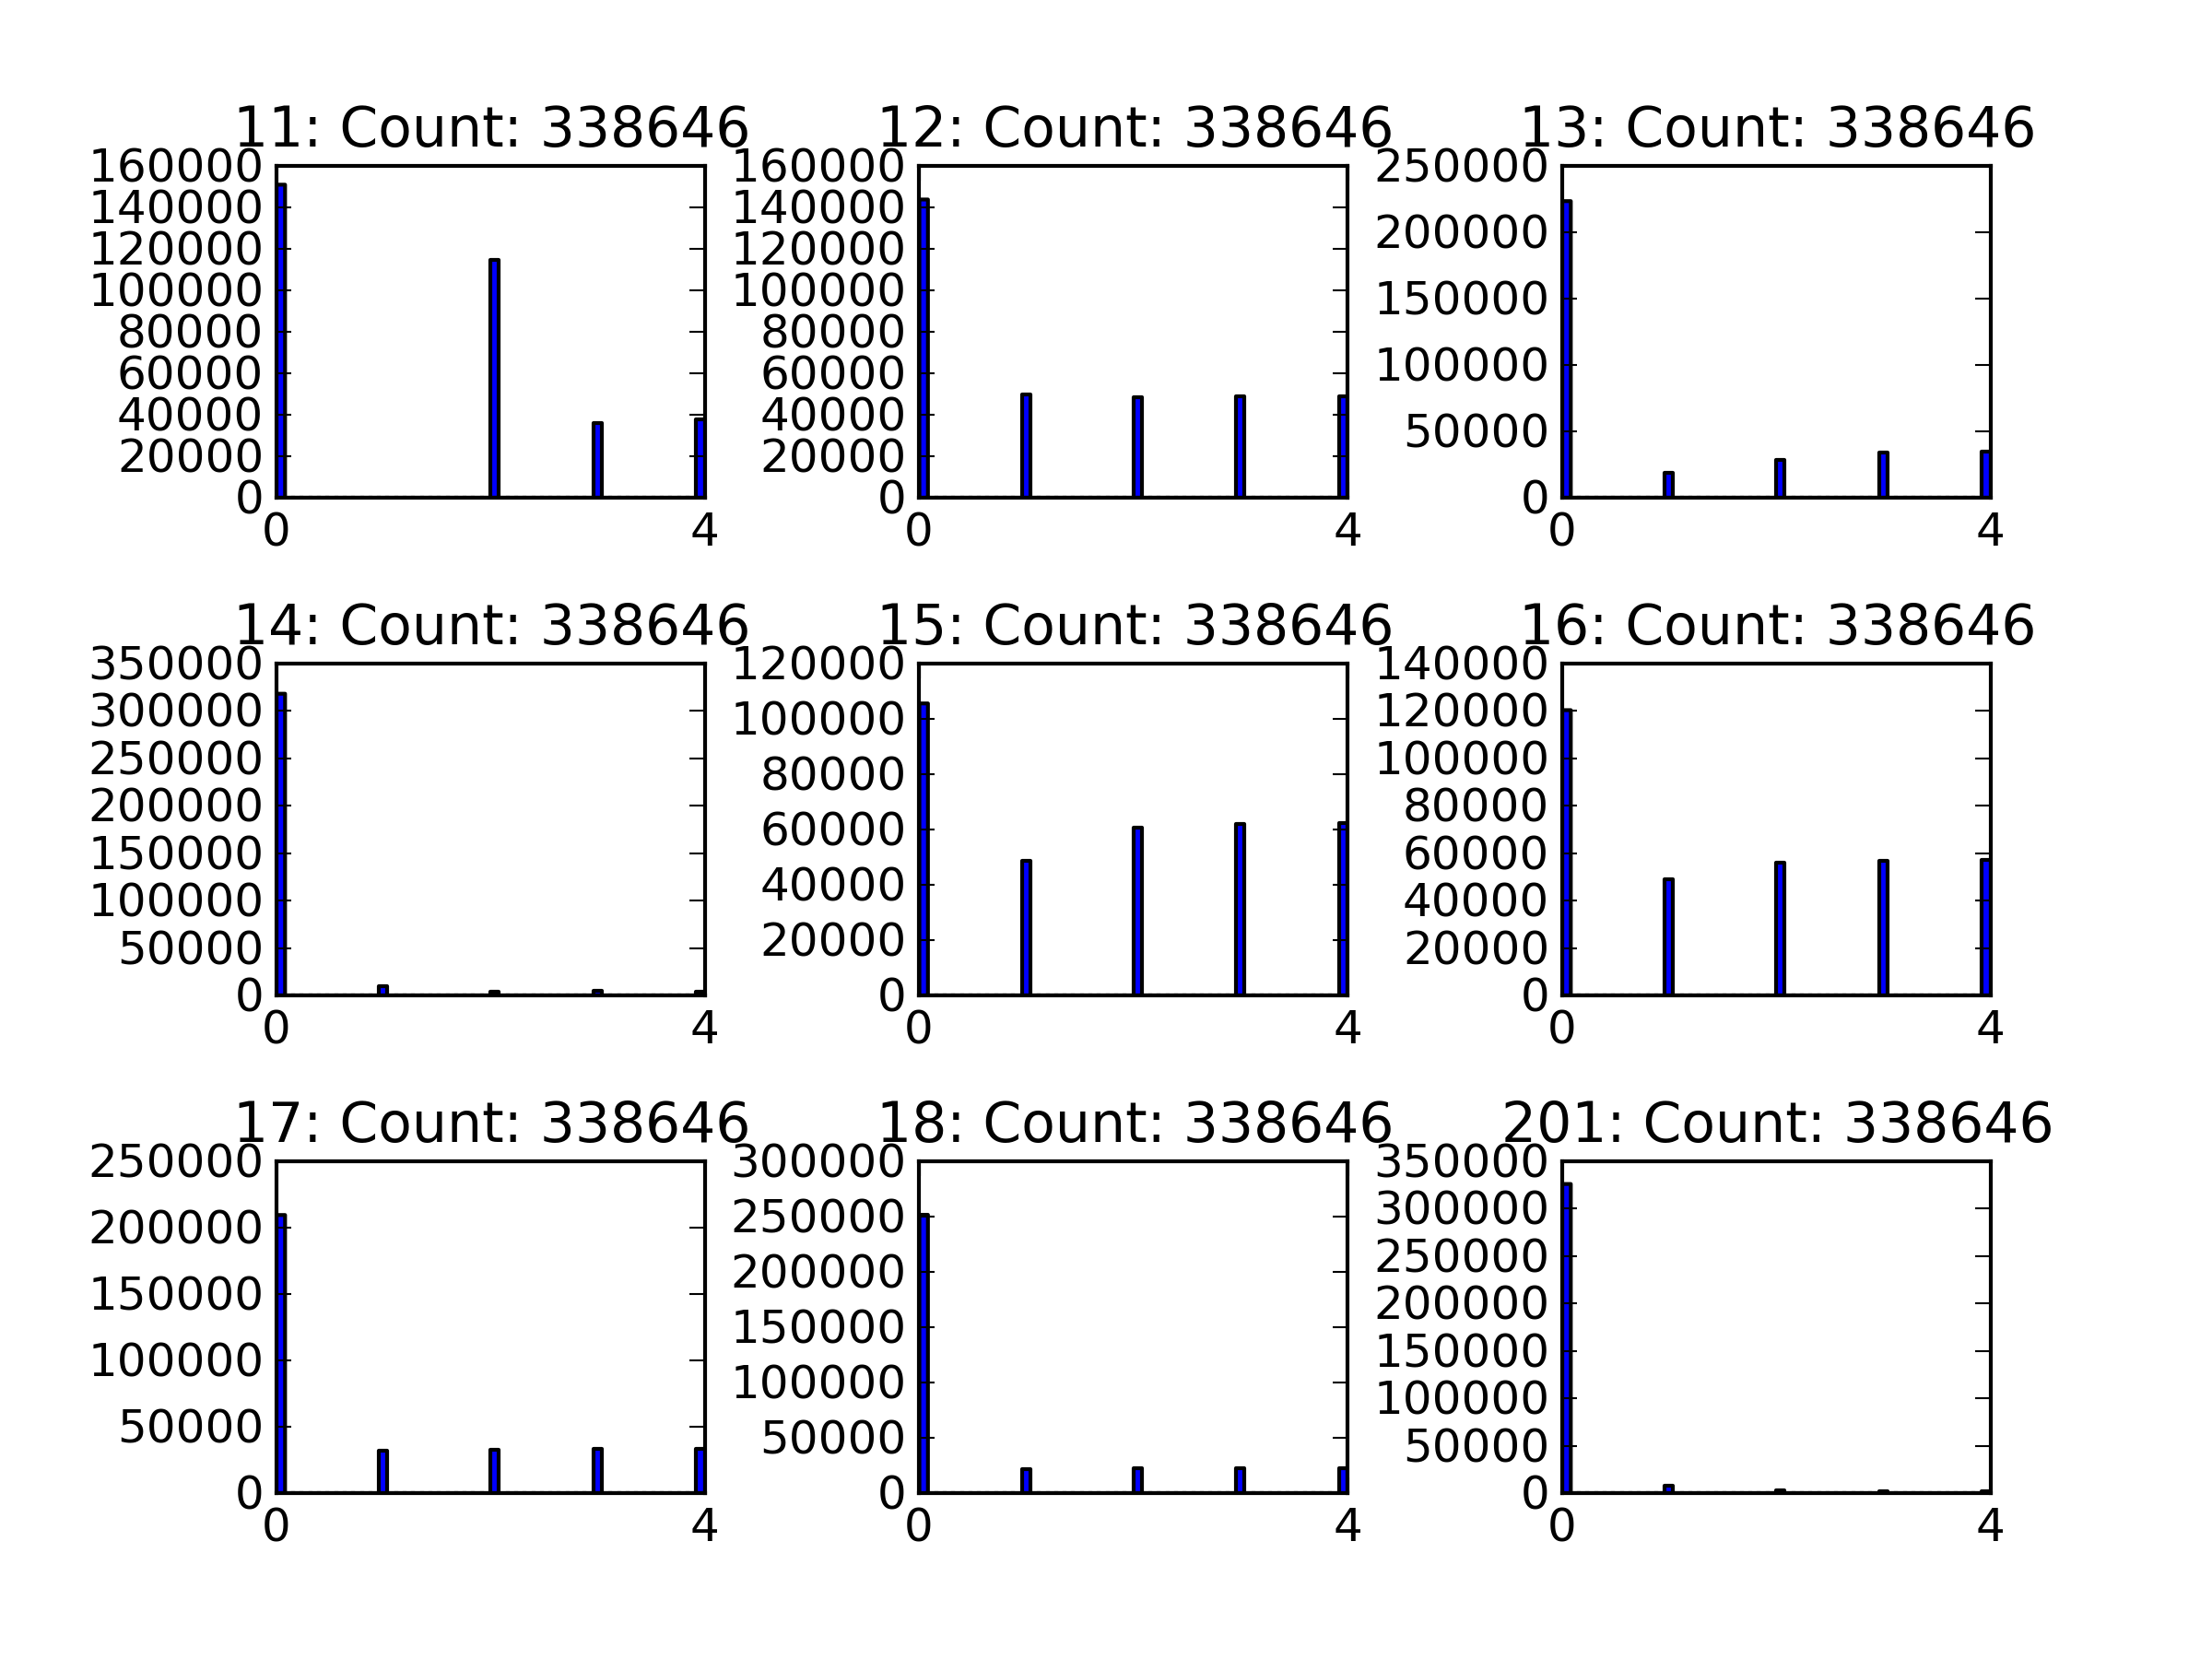
\includegraphics[width=1.0\textwidth]{figures/feature_distributions/features_bin_5_11_19.png}
\end{figure}

\begin{figure}[ht!]
  \caption{The distribution of binned feature values for \x{202} through \x{210}}\label{fig:features_bin_5_20_28}
  \centering
    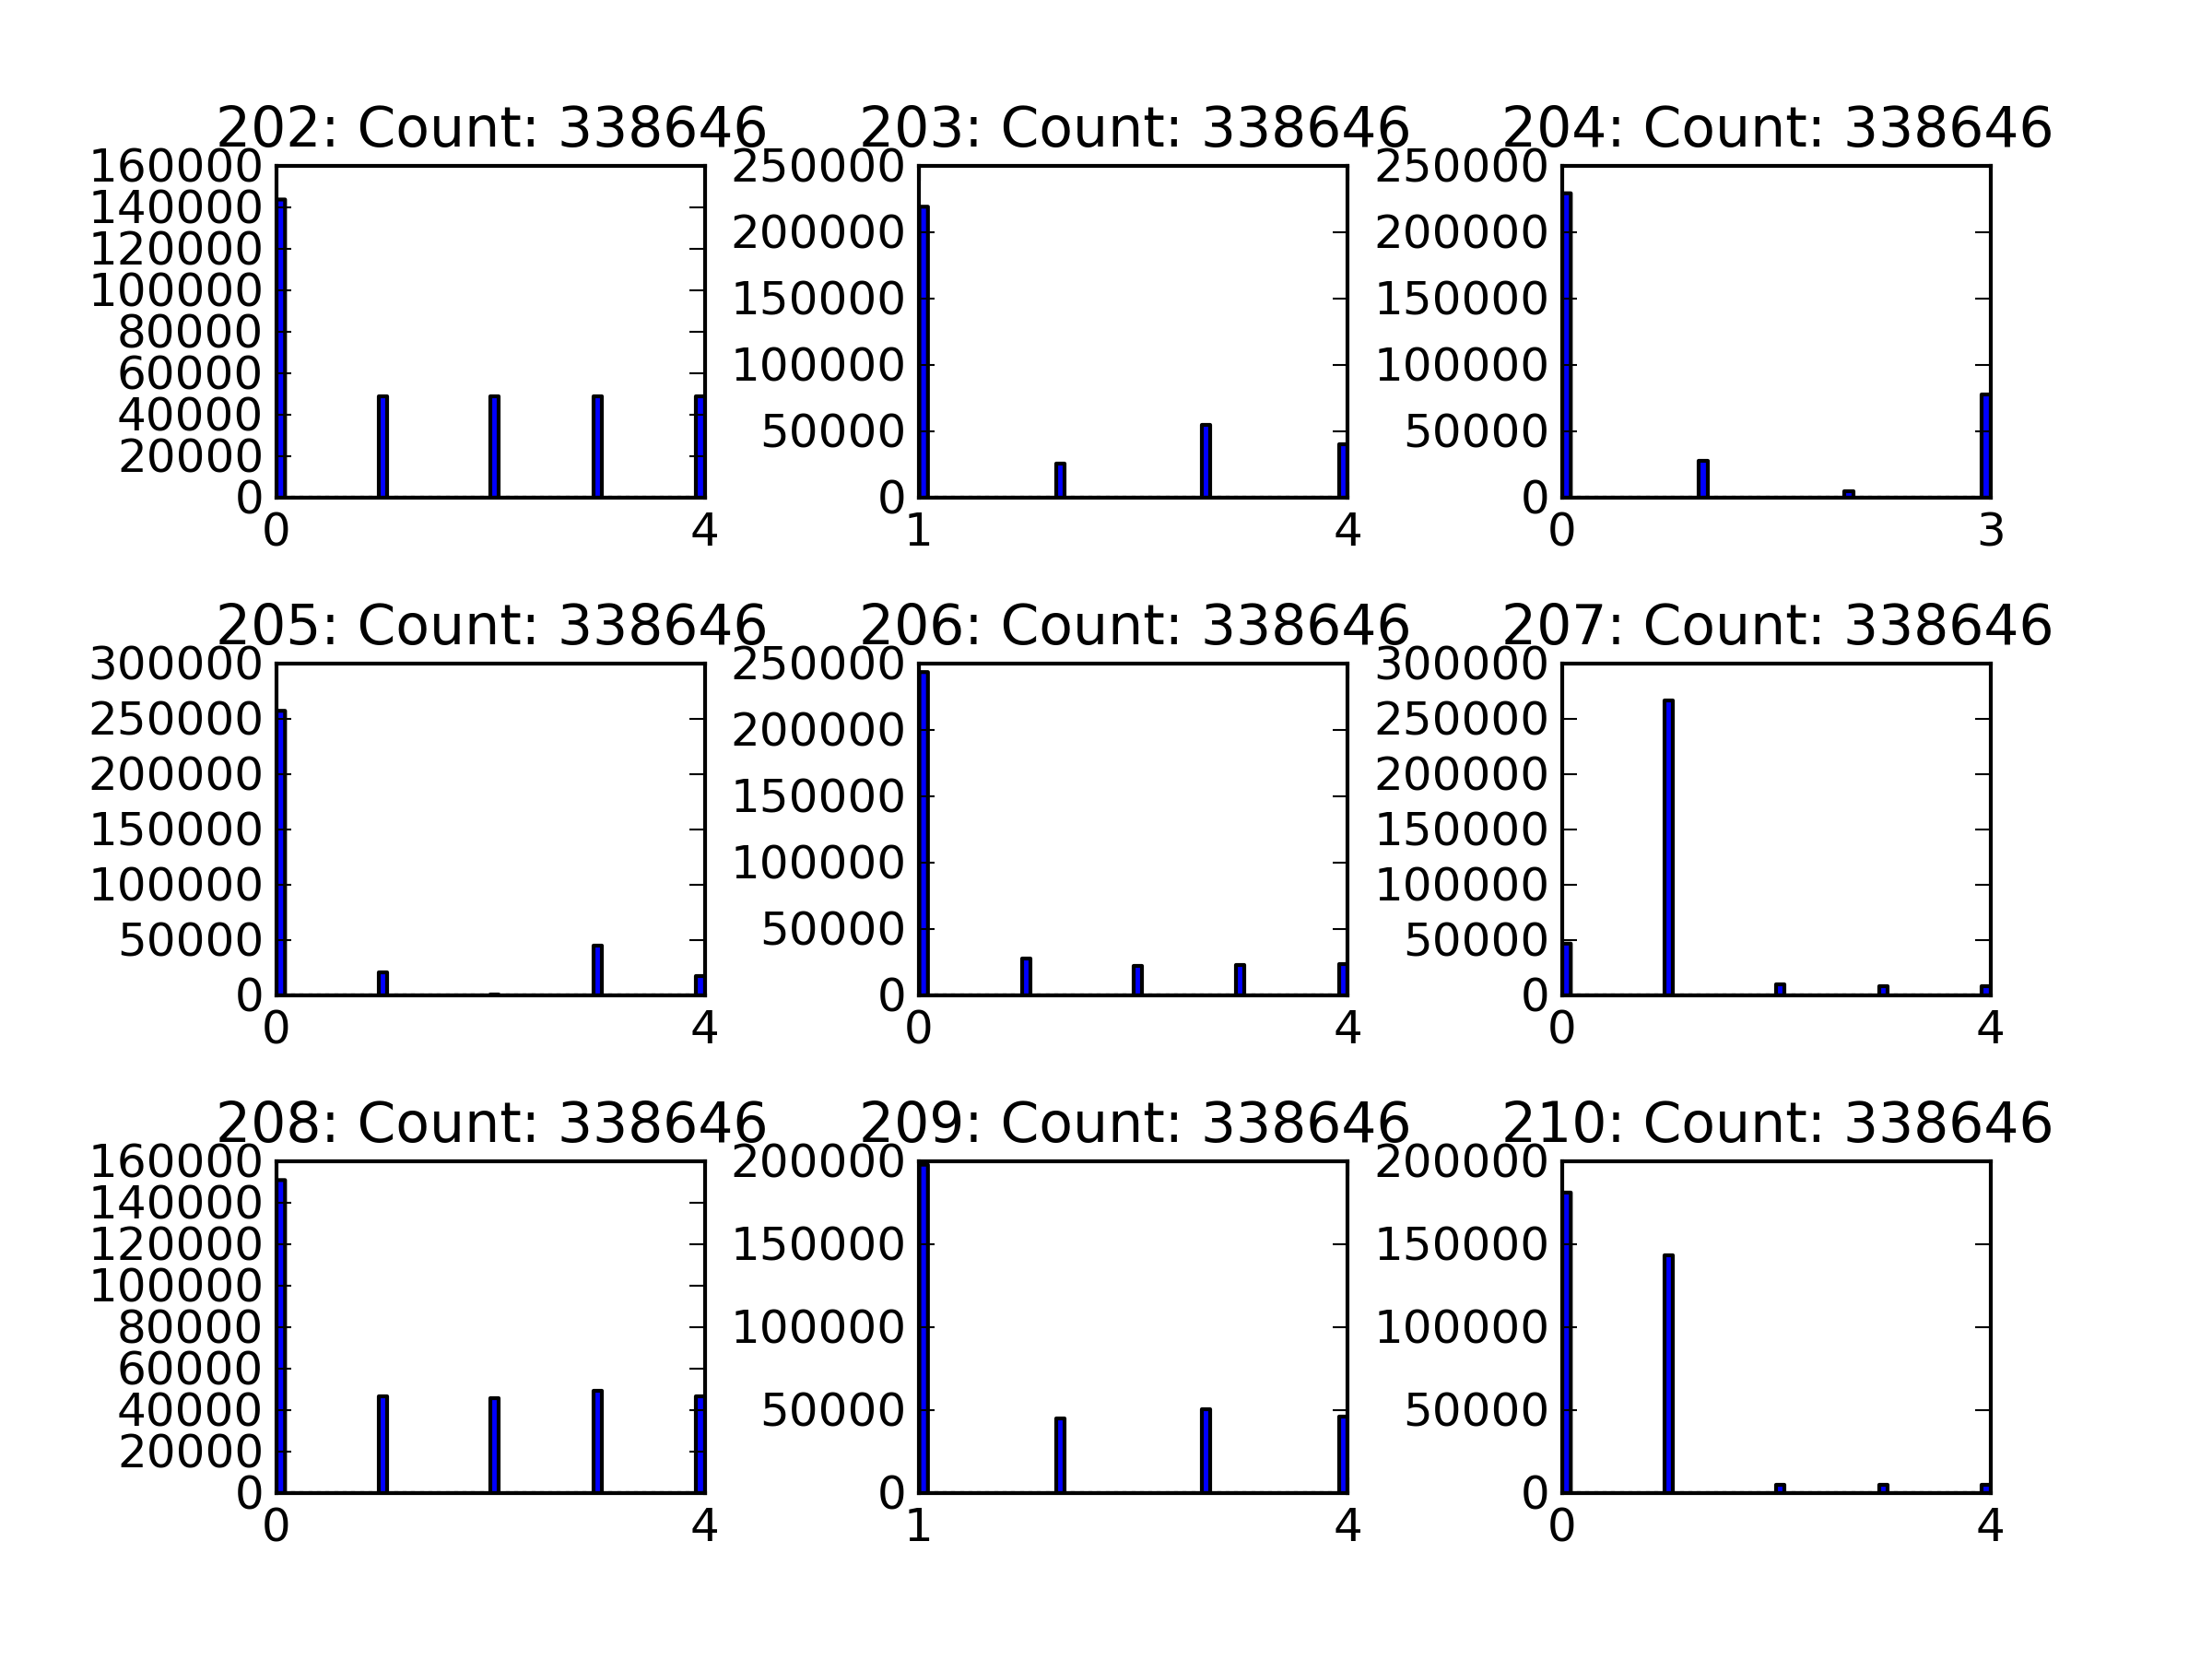
\includegraphics[width=1.0\textwidth]{figures/feature_distributions/features_bin_5_20_28.png}
\end{figure}

\chapter{Model Evaluation}\label{chap:evaluation}
In working with prediction problems, such as \sti prediction, there are many ways to evaluate how well a classifier (a.k.a. model) performs. In this chapter, we will briefly summarize the evaluation possibilities for a binary classification problem, and discuss why we chose the receiver operating characteristic as our primary metric.

\section{Point metrics for hard decision outputs}
When a classifier produces a hard decision output, i.e. a binary label, we evaluate the classifier using the following metrics.

\subsection{Confusion Matrices}
Generally, the evaluation measures in classification problems form a matrix with the numbers of examples correctly and incorrectly classified for each class, named the confusion matrix. The confusion matrix for a binary classification problem (which has only two classes - positive and negative), is defined by correct and incorrect classifications of positive and negative values. In our case, because we hope to predict \sti, a positive example represents \sti, and a negative example represents staying in the course. Table~\ref{table:confusion_matrix} shows the confusion matrix.
\newcommand\MyBox[2]{
  \fbox{\lower0.75cm
    \vbox to 1.7cm{\vfil
      \hbox to 1.7cm{\hfil\parbox{1.4cm}{#1\\#2}\hfil}
      \vfil}%
  }%
}


\noindent
\renewcommand\arraystretch{1.5}
\setlength\tabcolsep{0pt}

\begin{table*}[htp]
	\centering
	\caption{Dropout Prediction Confusion Matrix}\label{table:confusion_matrix}
	\begin{tabular}{c >{\bfseries}r @{\hspace{0.7em}}c @{\hspace{0.4em}}c @{\hspace{0.7em}}l}
	  \multirow{10}{*}{\parbox{1.1cm}{\bfseries\raggedleft actual\\ value}} & 
	    & \multicolumn{2}{c}{\bfseries Prediction outcome}\\
	  & & \bfseries stopout & \bfseries persist  \\
	  & stopout & \MyBox{True}{Positive} & \MyBox{False}{Negative} \\[2.4em]
	  & persist & \MyBox{False}{Positive} & \MyBox{True}{Negative}  \\
	\end{tabular}
\end{table*}



\begin{itemize}
\item True Positives (TP) are students who we correctly predict as stopping out.
\item False Positives (FP) are students who we predict will \sti, but who stay in the course.
\item False Negatives (FN) are students who we predict will stay in the course, but who actually stopout.
\item True Negatives (TN) are students who we correctly predict as staying in the course.
\end{itemize}

\subsection{Prediction Accuracy}
The simplest evaluation metric is prediction accuracy, which represents how often the classifier correctly predicted an example. A classifier's accuracy is given by $\frac{TN + TP}{FN + FP + TN + TP}$ Prediction accuracy can be applied to any classifier.

When the dataset is skewed towards one label or another, this becomes problematic because the optimal threshold to maximize accuracy favors the more likely label, and the classifier is able to achieve good accuracy by always guessing the more likely choice. This is the case in our dataset, as in any given week, more students stay in the class next week than stopout. If, for example, we are trying to predict one week ahead, and 90\% of students are still in the class next week, then a classifier can achieve 90\% accuracy by simply always predicting that a student will stay in. In addition to this problem, prediction accuracy loses information about the certainty of the answer, as it only outputs the label. For these reasons, prediction accuracy is not the primary metric we use to evaluate our models.

\subsection{Precision and Recall}
In a classification context, precision and recall are additional metrics for how well a classifier performs. Both are defined through equations relating confusion matrix values. 
Precision is given by $\frac{TP}{TP + FP}$. Intuitively, precision represents the accuracy of the classifier among those it classifies as positive examples. In our case, this becomes the fraction of students who were predicted to \sti and actually did leave the course.
Recall is given by $\frac{TP}{TP + FN}$. Intuitively, recall represents how good a classifier is at finding positive examples. In the \sti problem, recall represents the number of stopped out students the classifier is able to identify. A classifier with low recall allows many \sti students to fall through the cracks and escape detection.

For classifiers (such as logistic regression and Hidden Markov Models, classifiers which we use) that give the probability of being in each class, prediction accuracy and the precision recall point require picking a threshold to compare against. For example, for a threshold of 0.7, a classifier could predict that a student will stay in the course if the probability of staying is greater than 0.7. For this reason, this type of metric is called a point metric, or hard decision classification.

\section{Area metrics for soft decisions}
A more comprehensive metric to evaluate classifiers uses every threshold for evaluation. Models that generate a posterior probability estimate for a label are able to do this. An example of an area metric is the precision-recall curve.

\subsection{Precision-recall curve}
Although precision and recall are defined by a confusion matrix, in practice they are often represented as possible precision and recall scores as a classifier sweeps through threshold values. Of course, this sweeping only applies to classifiers which give a probability of being in each class. This produces a precision-recall curve, which graphs possible precision values vs. possible recall values during this threshold sweep. Figure \ref{fig:example_precision_recall} shows an example curve. Each point on the curve represents a threshold. The AUC, or area under the curve, is a simple, one-number metric which represents how well the classifier performs over all thresholds. The precision-recall curve is commonly used in evaluating predictive models.

\begin{figure}[ht!]
  \caption{Example precision-recall curve. The curve was generated using logistic regression on the forum\_only dataset, with a lead of 3 and a lag of 4. This model will be discussed later, but serves here as an example.}\label{fig:example_precision_recall}
  \centering
    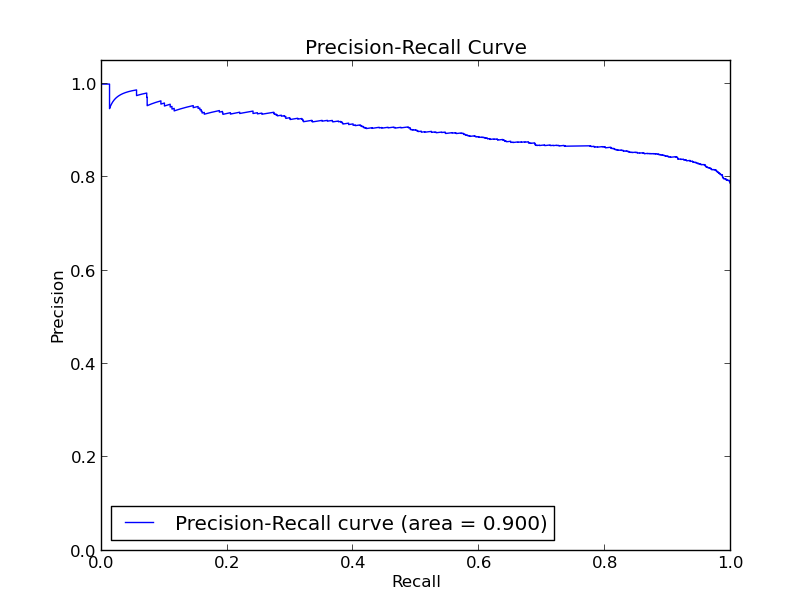
\includegraphics[width=1.0\textwidth]{figures/example_precision_recall.png}
\end{figure}

\subsection{Receiver Operating Characteristic}
Another widely used metric of classifier performance is called the receiver operating characteristic. Like the precision-recall curve, the receiving operating characteristic, or ROC, is a line representing the performance as a classifier sweeps a range of thresholds of decision boundaries. Figure \ref{fig:example_roc} shows an example ROC curve. The ROC curve represents the range of possible probability of False Alarm and probability of Detection values. Both probability of False Alarm (pFA) and probability of Detection (pD) are given by confusion matrix quantities.
pD is equal to $ \frac{TP}{TP + FN}$. This is equivalent to recall, and represents how good a classifier is at finding positive examples.
pFA is equal to $ \frac{FP}{FP + TN}$. This represents how likely a classifier is to mistakenly classify a negative example as a positive one.

\begin{figure}[ht!]
  \caption{Example ROC curve. The curve was generated using logistic regression on the forum\_only dataset, with a lead of 3 and a lag of 4. This model will be discussed later, but serves here as an example.}\label{fig:example_roc}
  \centering
    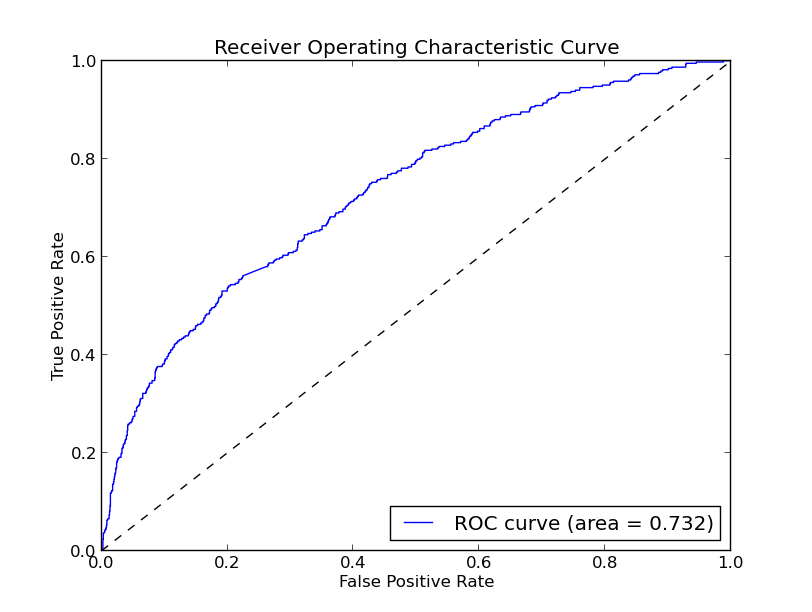
\includegraphics[width=1.0\textwidth]{figures/example_roc.png}
\end{figure}

Like precision and recall, a receiver operating characteristic is useful because it describes a classifier's ability over a wide range of thresholds. Indeed, both are very similar, and in a way equivalently useful for describing a classifier. Which curve to use depends on which value is more important in a prediction problem, which is usually context specific. We choose to use the receiver operating characteristic.

The integral of the ROC curve produces a one-number metric called the area under the curve (AUC). Like the AUC of precision-recall, it concisely describes a classifier, and is the primary metric we use as we compare predictive models. As previously noted, a lot of information is packed into this one number, and thus is a convenient summary of the effectiveness of the model.

\section{Training and Testing}
In order to independently construct and evaluate our models, we divided each cohort's dataset into a mutually exclusive train dataset and test dataset. We chose a 70\% train, 30\% test split, meaning that 70\% of each cohort's data was put into a train dataset, and the remaining was put into a test dataset. In each of our predictive models, we only used the train dataset to build the model, and ultimately evaluated it (using the aforementioned receiver operating characteristic metrics) on the test dataset to determine the model's performance. The test dataset represent previously unknown, sampled data from the population of students, and was never used until the final evaluation of the models.

In order to preserve the distribution of students as best as possible, we aimed to keep the 70/30 split for each stopout week for each cohort. In other words, for each cohort, we split the students who stopped out in week 1 70/30, then split students who stopped out in week 2 70/30, and so on, for each \sti week. In order to achieve that split, we iterated through the overall file, and put students into the appropriate dataset as they appeared so as to constantly keep the 70/30 split over each student. We did so in this way as to not bias the split from the ordering of our file. In other words, neither the train nor test split has a bias towards students who registered for the class earlier. The results are training and testing datasets for each cohort, each of which are proportional to the aggregate cohort in terms of the stopout weeks of the students and student registration times.

\section{Cross validation}
We employed a technique called cross validation in all of our predictive modelling. Cross validation tests a predictive model without the test dataset, in order to gauge when a model might be over-fitting, and to gauge sensitivity in model accuracy from data sensitivity. Some partitions are used in constructing a model, and others are used to evaluate the model's performance. Specifically, we used K-fold cross validation. K-fold cross validation is a commonly used technique which randomly divides the dataset into K folds (or partitions). Cross validation then constructs K models. Each model is constructed using K-1 of the folds, and the model is evaluated using the last unused fold. Figure \ref{fig:cross_validation} shows a diagram of this. K-fold cross validation helps to protect against over-fitting, and provides an alternative and complimentary evaluation metric to the test dataset. Cross validation, and K-fold cross validation are commonly used in practice. In our evaluations, we employ 10 fold cross validation and use the average of the ROC AUC over the folds as another evaluation metric.

\begin{figure}[ht!]
  \caption{The k-fold cross validation partitioning. K models are built, using K-1 folds for model construction and the last fold for model evaluation}\label{fig:cross_validation}
  \centering
    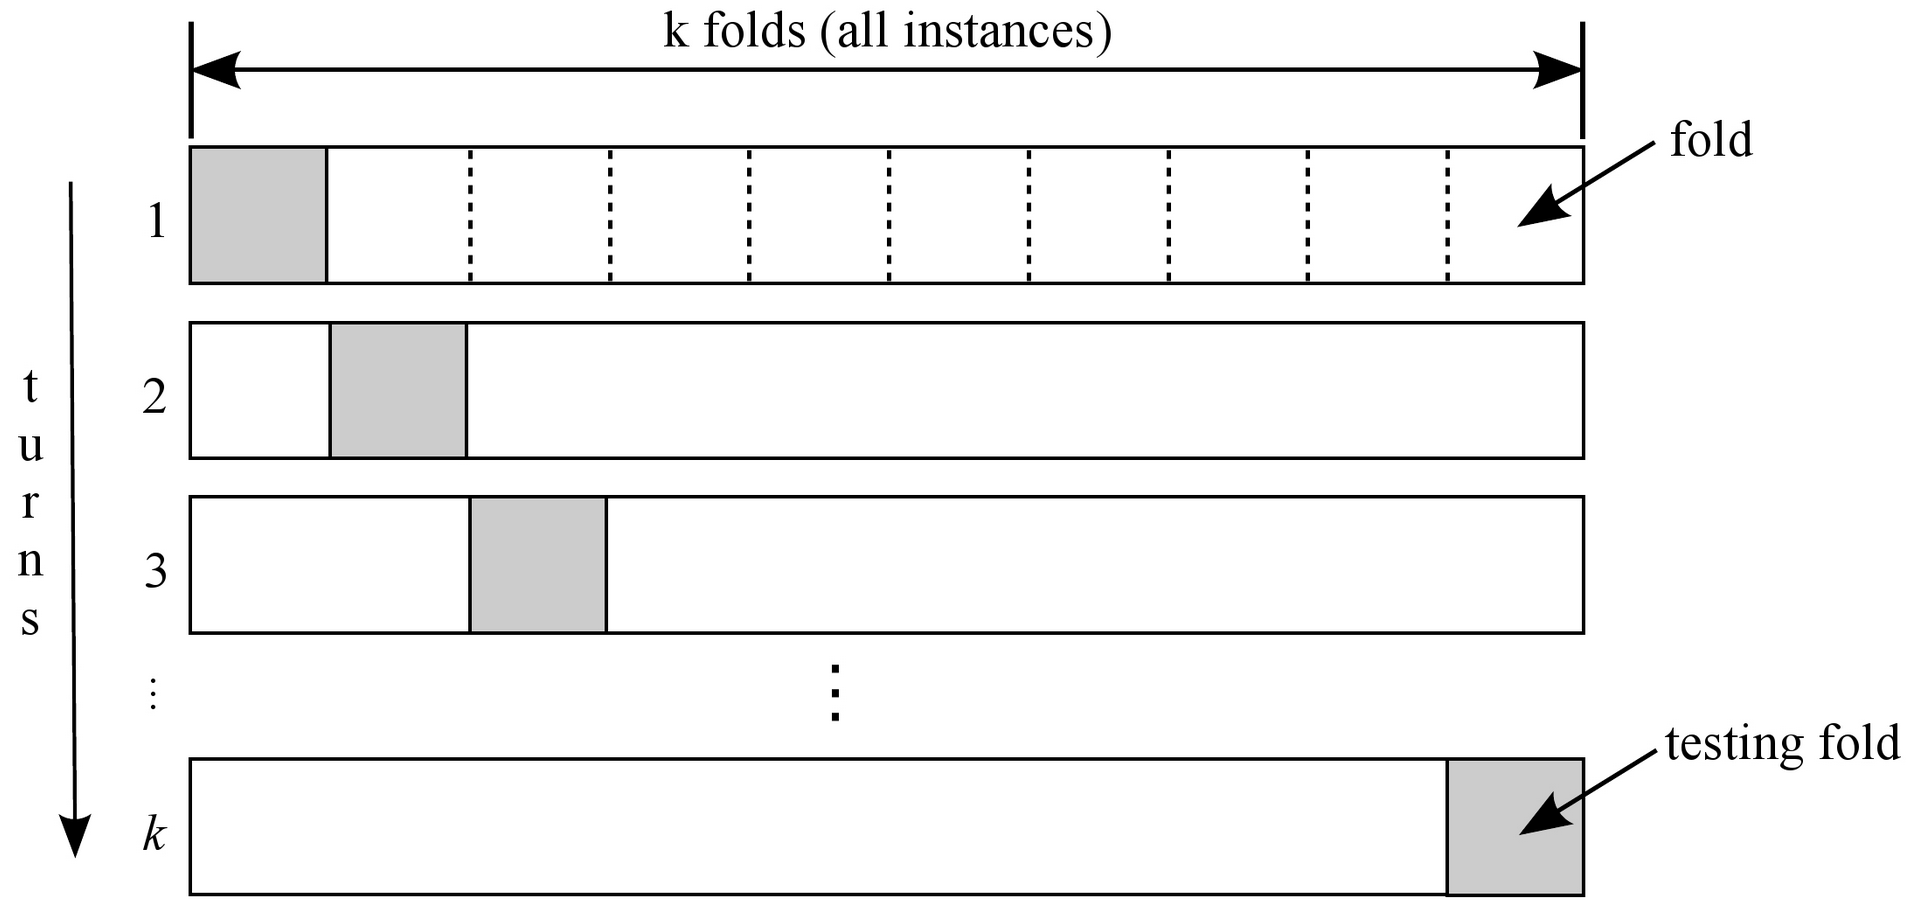
\includegraphics[width=1.0\textwidth]{figures/cross_validation.png}
\end{figure}
\chapter{Discriminative Models to Predict Stopout} \label{chap:logreg}

In the Chapter \ref{chap:features} we presented the feature extraction process, where a feature represents student behavior on a weekly basis. There are $m$ \feat per student, which we assemble as shown in the figure below: 

\begin{figure}[ht!]
  \caption{The feature matrix, which captures each feature value for each week. Each student has such a matrix.}\label{fig:student_weekly_features}
  \centering
    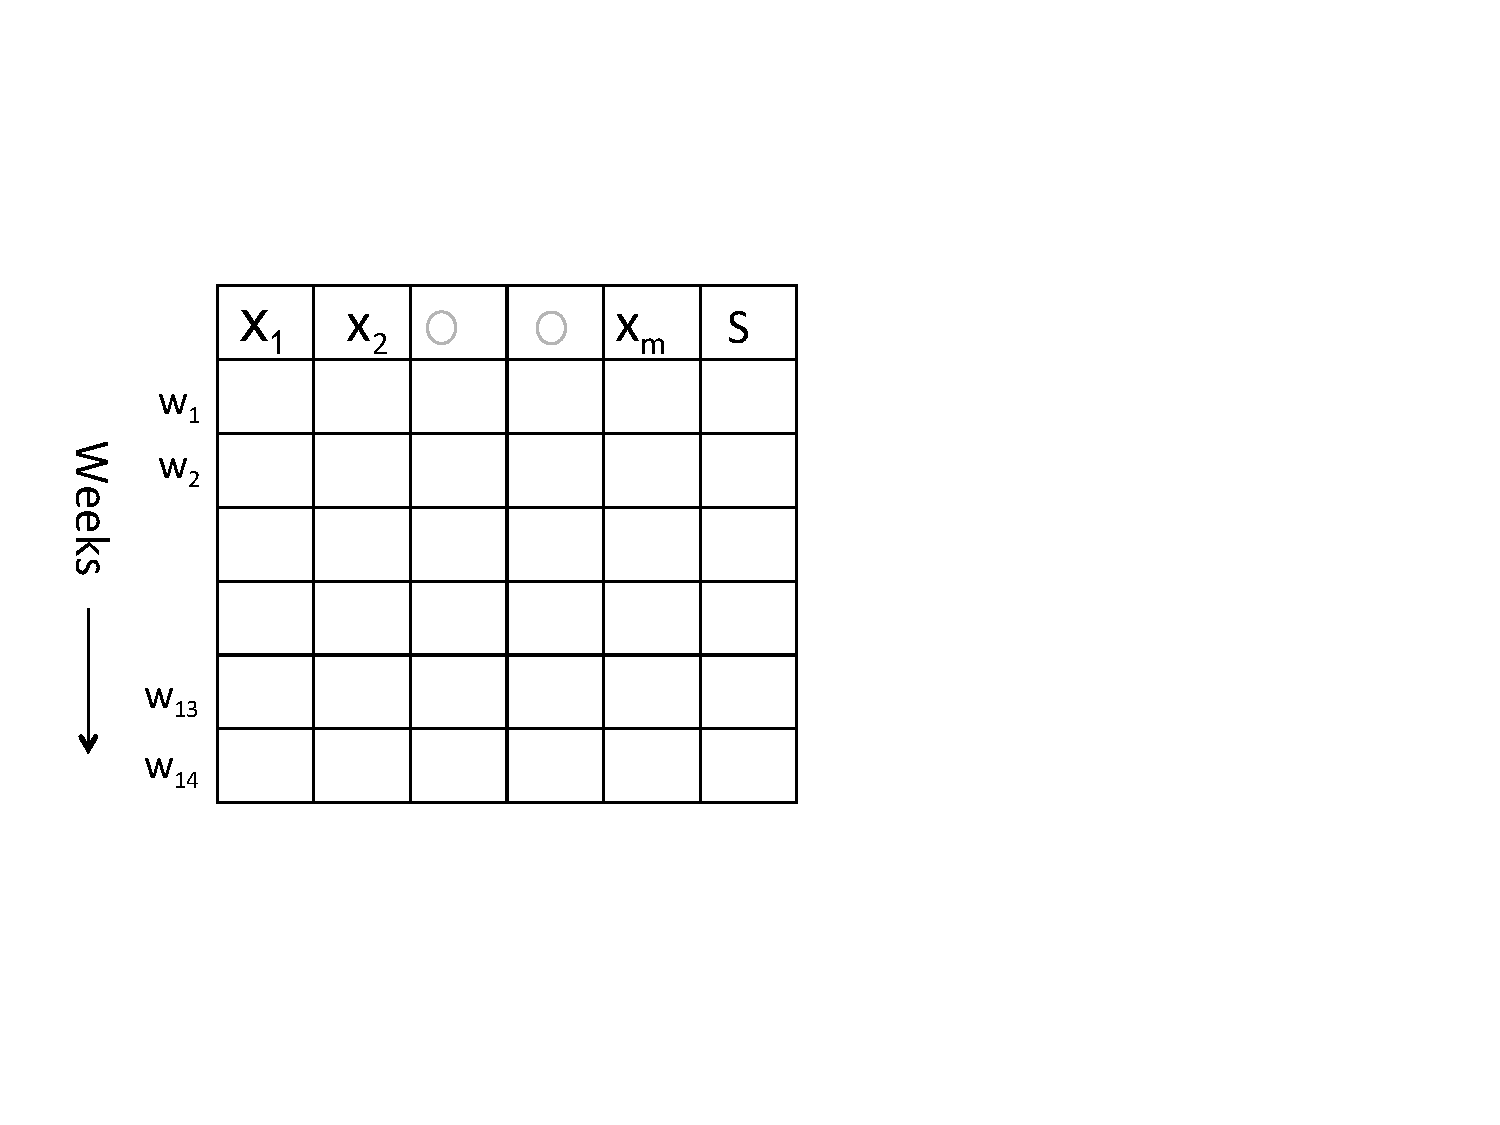
\includegraphics[width=0.5\textwidth]{figures/student_week_matrix}
\end{figure}

To illustrate the predictive model's potential application, we will use a realistic scenario. The model user, likely an instructor or platform provider, could use the data from week 1 to week $i$ (current week) to make predictions. The model will predict existing student \sti during weeks $i+1$ to $14$. For example, Figure~\ref{fig:lead_lag2} shows one such prediction problem. In this case the user, currently at the end of week 3, is attempting to predict \sti for the 8th week. 
\begin{figure}[!ht]
  \caption{Diagram of the student's weeks data used in a lead 5, \lag 3 prediction problem}\label{fig:lead_lag2}
  \centering
    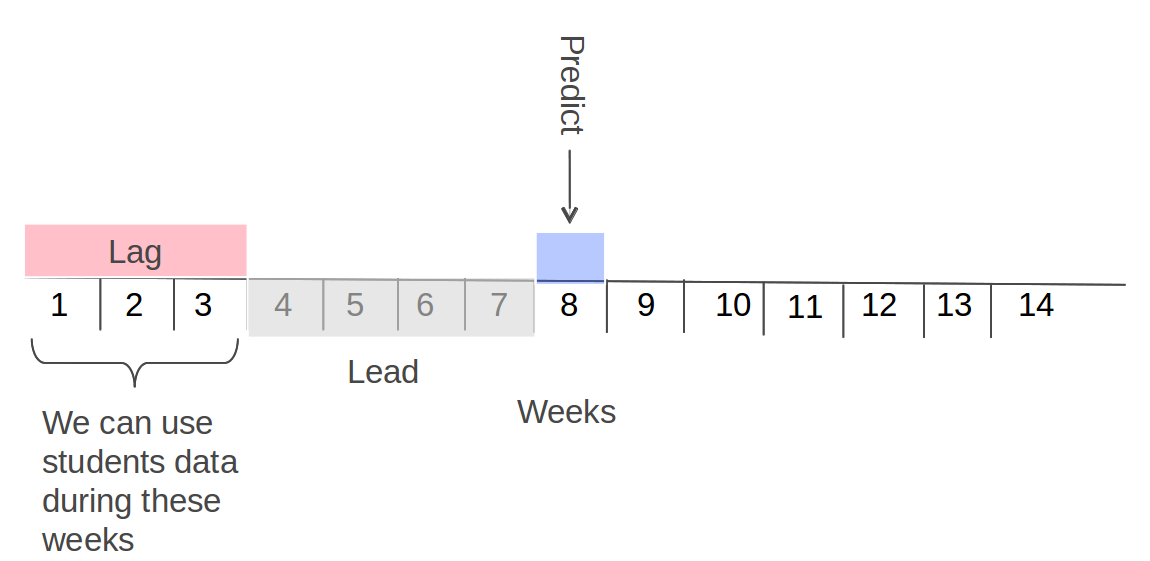
\includegraphics[width=1.0\textwidth]{figures/lead_lag.png}
\end{figure}

\begin{figure}[ht!]
  \caption{Diagram of the flattening process. In this case two weeks of data is used to predict week 13. This prediction problem corresponds to a lead of 11, and a lag of 2.}\label{fig:flattening}
  \centering
    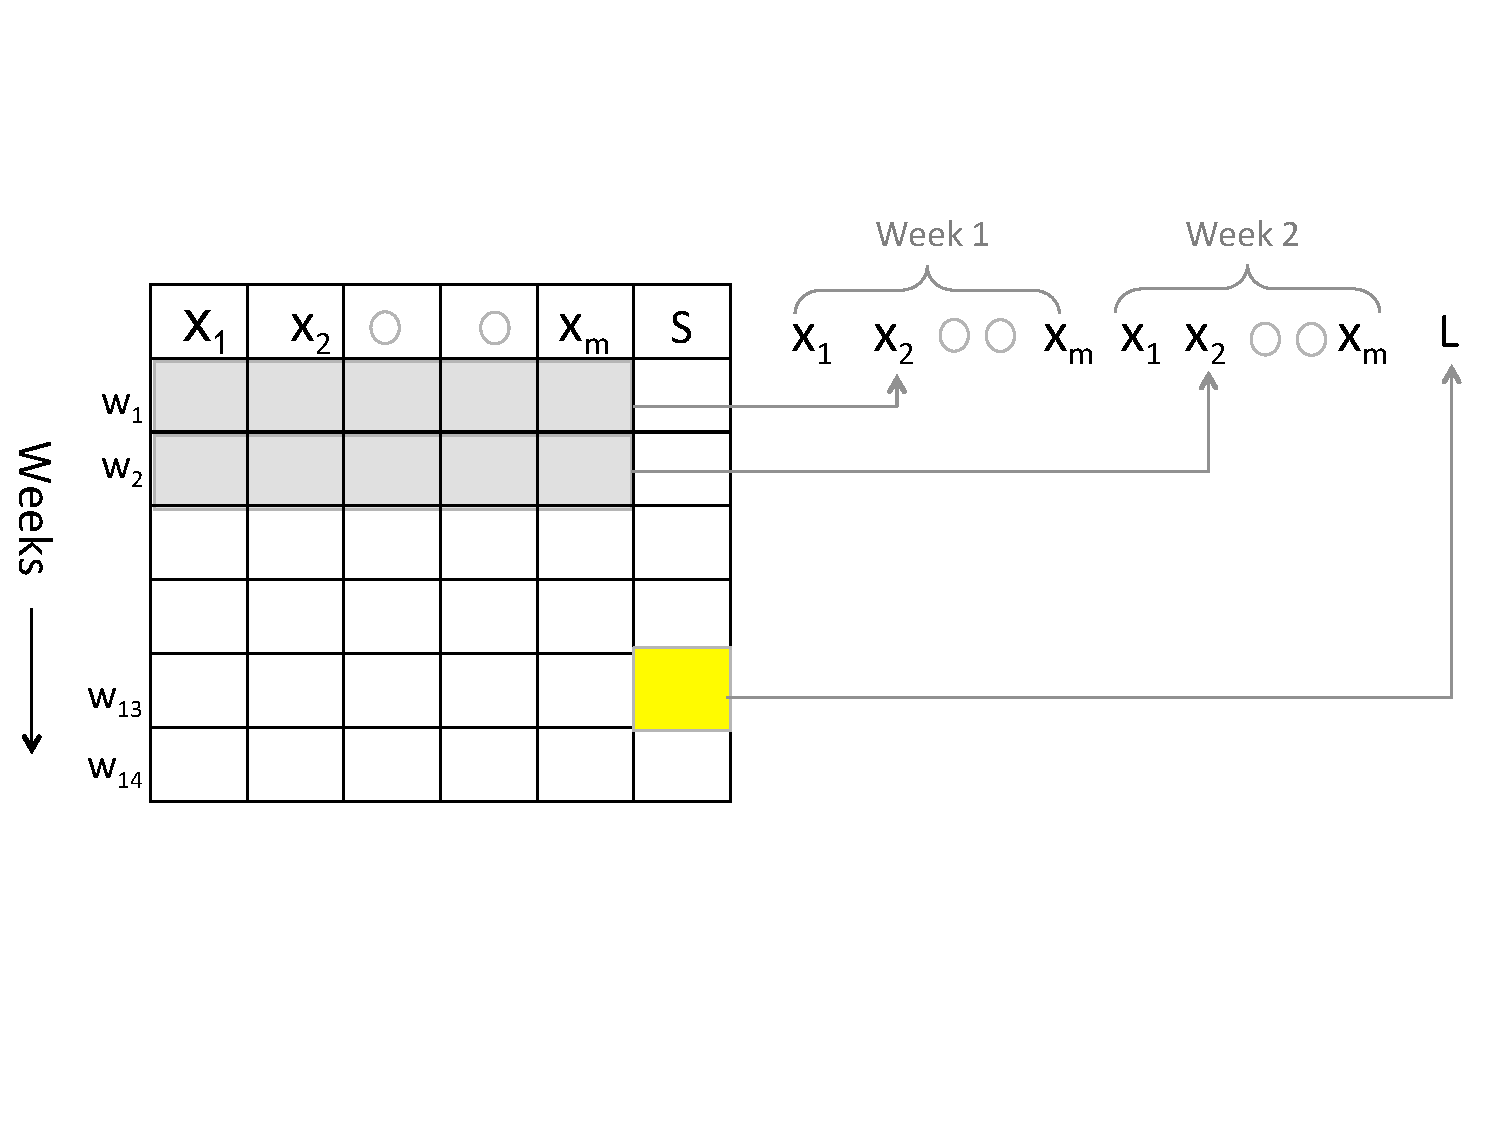
\includegraphics[width=0.7\textwidth]{figures/Flattening}
\end{figure}

\paragraph{Multiple prediction problems}\label{para:multiple_prediction}
Under this definition 91 individual prediction problems exist. For any given week $i$ there are $14-i$ number of prediction problems. Each prediction problem becomes an independent modeling problem which requires a discriminative model. To build discriminative models we utilize a common approach of flattening out the data, that is forming the \cov for the discriminative model by assembling the features from different student-weeks as separate variables. This process is shown in Figure~\ref{fig:flattening}. The example uses data from weeks 1 and 2 (lag of 2) and attempts to predict the \sti for week 13 (lead of 11). 

In this chapter, we present a logistic regression method for building several predictive models. In each of the following sections, we present a model, its advantages and how it is learned. Furthermore, we present a logistic regression variant called randomized logistic regression which we employ to identify feature importance. In Chapter~\ref{chap:delphi} we present results from numerous other approaches for discriminative modeling. 

\section{Logistic Regression}
Logistic regression is a commonly used binary predictive model. It calculates a weighted average of a set of variables, submitted as \cov, as an input to the \textit{logit} function. Thus, the input to the \textit{logit} function, z, takes the following form:
\begin{equation}
 z = \beta_0 + \beta_1 * x_1 + \beta_2 * x_2 + ... \beta_m * x_m  %note N is always reserved for the total number of examples 
 \end{equation}
Here, $\beta_1$ to $\beta_m$ are the coefficients for the feature values, $x_1$ to $x_m$. $\beta_0$ is a constant. The \textit{logit} function, given by, 
\begin{equation}\label{eq:logit}
 y = \frac{1}{1 + e ^{-z}}
 \end{equation}
takes the shape as shown in figure \ref{fig:logit}. Note that the function's range is between 0 and 1, which is optimal for probability. Also note that it tends to `smooth out' at extreme input value, as the range is capped. 

\begin{figure}[ht!]
  \caption{The logit (aka logistic or sigmoid) function. The logit equation is $ y = \frac{1}{1 + e ^{-x}}$. The range of the function is between 0 and 1.}\label{fig:logit}
  \centering
    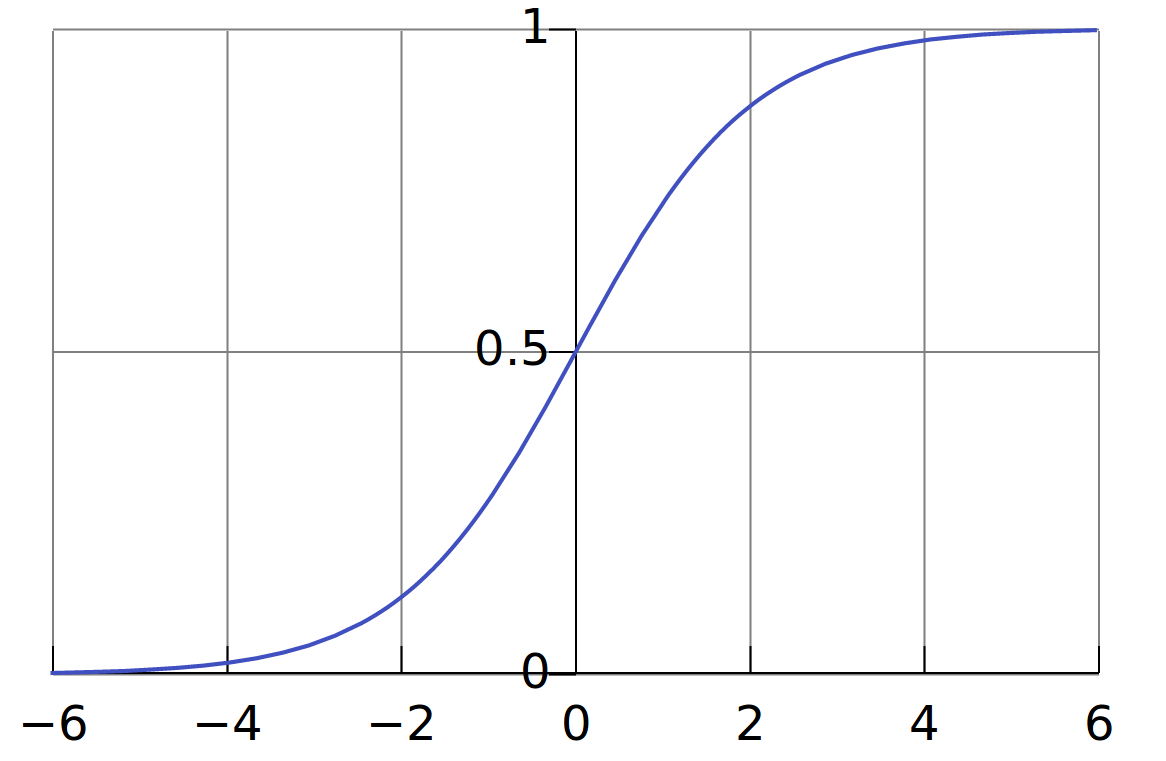
\includegraphics[width=0.7\textwidth]{figures/logit.png}
\end{figure}

For a binary classification problem, such as ours, the output of the \textit{logit} function becomes the estimated probability of a positive training example. These feature weights, or coefficients, are similar to the coefficients in linear regression. The difference is that the output ranges between 0 and 1 due to the logit function, rather than an arbitrary range for linear regression.

\subsection{Learning}
The objective of training a logistic regression model is to find a set of coefficients well suited to fit the data. For the binary classification problem,  as noted before, training involves passing a set of \cov and a corresponding binary label associated with the \cov. After training a model, the predicted probability, or the output of the \textit{logit} function, should predict higher probabilities for the positive `+1' class examples in the training data and a lower probability for the negative `0' class examples. 

There is no closed form solution to find the optimal coefficients to best fit the training data. As a result, training is usually done iteratively through a technique called maximum likelihood estimation \cite{menard2002applied}. First, a random set of coefficients are chosen. At each iteration, an algorithm such as Newton's method is used to find the gradient between what the coefficients predict and what they should predict, and updates the weights accordingly. The process repeats until the change in the coefficients is sufficiently small. This is called convergence. After running this iterative process over all of the training examples, the coefficients represent the final trained model.

\subsection{Inference and evaluation}
With training in place, the next step is evaluating the classifier's performance. A testing set comprised of untrained \cov and labels evaluates the performance of the model on the test data following the steps below: 
\begin{description}\label{steps}
\item {Step 1:} The logistic function learned and presented in ~\ref{eq:logit} is applied to each data point and the estimated probability of a positive label $y_i$ is produced for each.

\item {Step 2:}  A decision rule is applied to determine the class label for each probability estimate $y_i$. The decision rule is given by: 
\begin{equation}\label{eq:decRule}
\hat {L_i} = \left\{ 1, \ if \ y_i \geq \lambda \atop 0, \ if \ y_i < \lambda \right\}
\end{equation}
Given the estimated labels for each data point $\hat{L_i}$ and the true labels $L_i$ we can calculate the confusion matrix, true positives and false positives and thus obtain an operating point on the ROC curve. 
\item {Step 3:} By varying the threshold $\lambda$ in \ref{eq:decRule} the decision rule above we can evaluate multiple points on the ROC curve. We then evaluate the area under the curve and report that as the performance of the classifier on the test data.
\end{description}

\begin{paragraph}
{Predictive accuracy heat map} To present the results for multiple prediction problems for different weeks simultaneously, as discussed in Section~\ref{para:multiple_prediction},  we assemble a heat map of a lower right triangular matrix as shown in Figure~\ref{fig:logistic_regression_heatmap_no_collab2}. The number on the x-axis is the week for which predictions are made of that experiment. The y-axis represents the \lag, or the number of weeks of data used to predict. The color represents the area under the curve for the ROC that the model achieved. Note that as the predicted week increases for a given \lag, it is harder to predict. Likewise, as we increase the \lag for a given prediction week, the stopout value becomes easier to predict. This implies that using more historical information enables a better prediction.
\end{paragraph}

\begin{figure}[!ht]
  \caption{Example heatmap for a logistic regression problem. The heatmap shows how the ROC AUC varied as \lag changed as the target prediction week changed.}\label{fig:logistic_regression_heatmap_no_collab2}
  \centering
    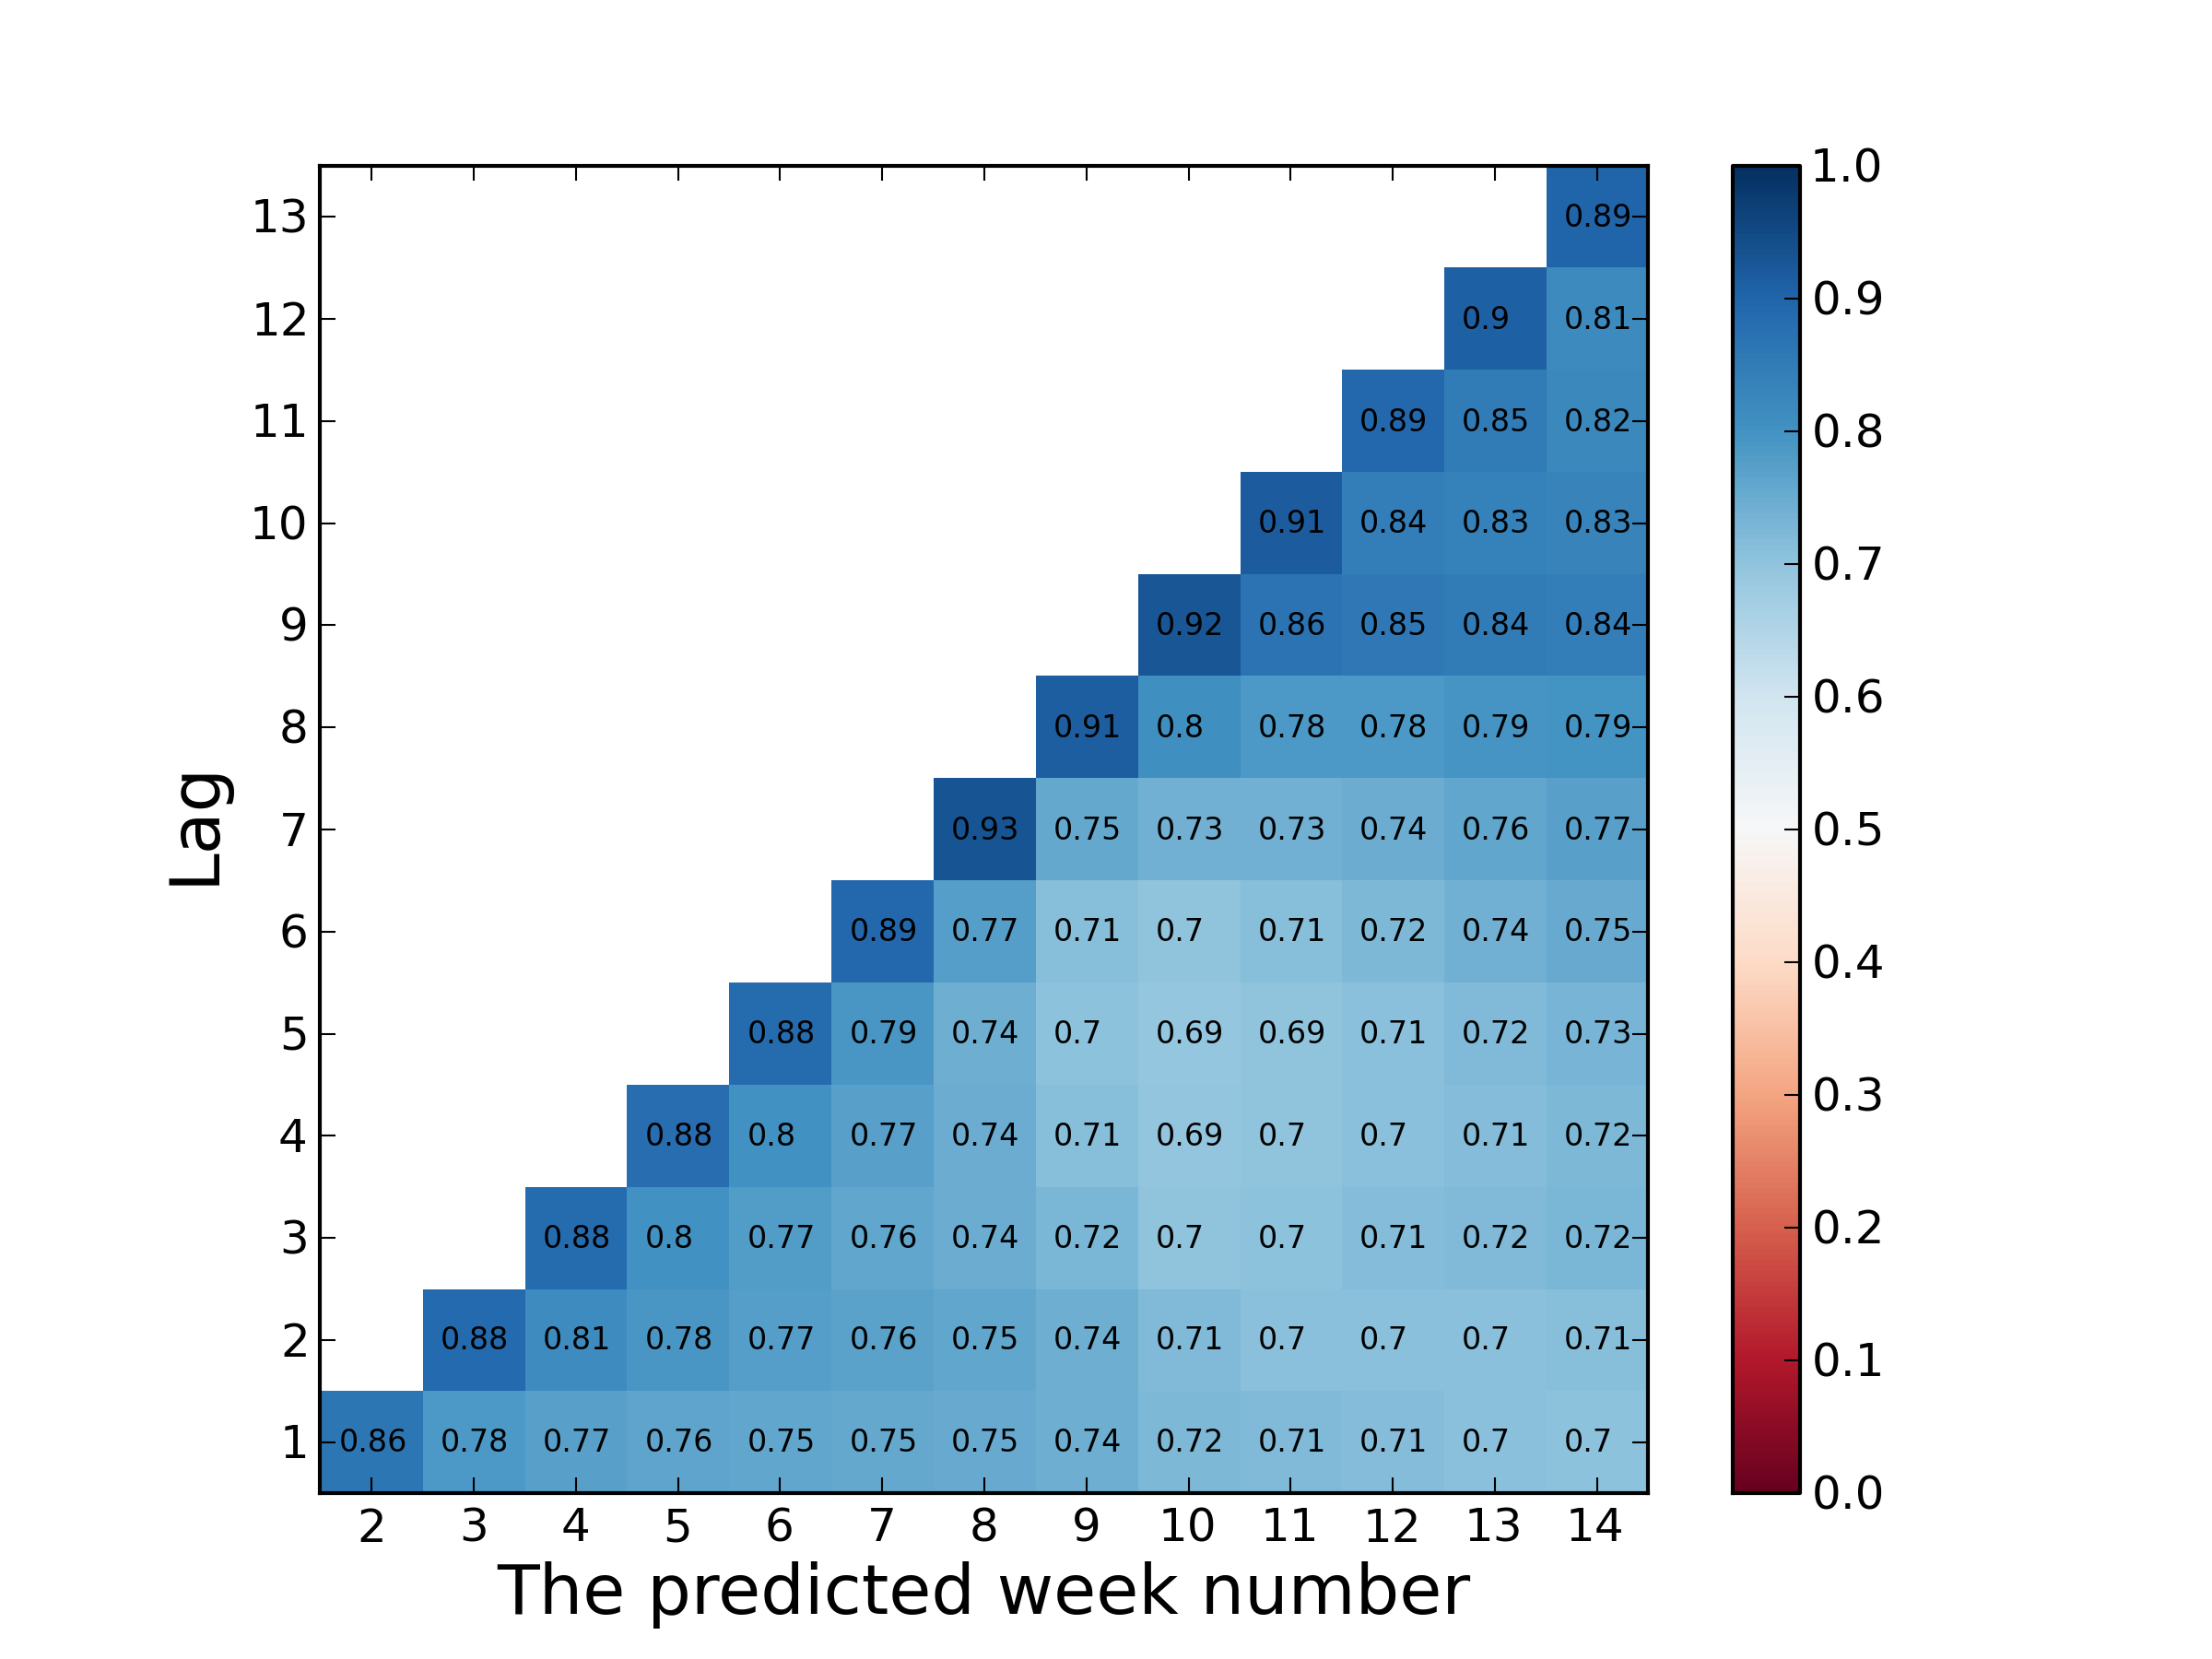
\includegraphics[width=0.8\textwidth]{figures/logreg/no_collab.png}
\end{figure}

\subsection{Attractive properties of logistic regression} 
\begin{itemize}
\item It is relatively simple to understand. 
\item After a model is trained, it provides feature weights, which are useful in assessing the predictive power of features (this will be discussed further in our treatment of the randomized logistic regression model). 
\item It is fast to run. On a single i-7 core machine, for example, running each of the 91 prediction problems on all 4 cohorts took ~25 hours.
\end{itemize}

\section{Predicting stopout with logistic regression}
We applied logistic regression to student persistence prediction. We used the 27 interpretive features as described in Chapter~\ref{chap:features} to form the feature vectors, and maintained the \sti value as the label. We used the features themselves, rather than the PCA features so as to analyze predictor importance.

\subsection{Experimental setup}
To perform logistic regression analysis, we executed the ensuing steps for every lead, \lag and cohort combination
\footnote{
We used the logistic regression implementation of an open source machine learning library, called scikit-learn. We chose this library because it is well known and tested, fast (the core maximum likelihood estimation algorithm is written in C), with an easy to use python interface. In addition, the scikit-learn library includes an easy interface for cross validation and feature normalization.}:
\begin{enumerate}
\item Performed 10 fold cross validation on the training set. As outlined in the evaluation chapter, this involved training the model on 9 folds of the train dataset and testing on the last fold.
\item Trained a logistic regression model on the entire train dataset.
\item Applied the model to the test dataset by putting each data point through the model then applying the decision rule in ~\ref{eq:decRule} and following the steps in ~\ref{steps} to determine the AUC under the ROC.
%the resulting probability of \sti versus the truth \sti label.
\item Evaluating the model using mean cross validation ROC AUC and test set ROC AUC.
\end{enumerate}

\subsection{Experimental results}
Figures \ref{fig:logistic_regression_heatmap_no_collab} through \ref{fig:logistic_regression_heatmap_wiki_only} summarize the AUC of the receiver operating characteristic for all four cohorts over each lead and \lag combination. Overall, logistic regression predicted dropout with very high accuracy. Some experiments, such as a \lag of 7, predicting week 8 in the \both cohort achieved accuracies as high as 0.95, a fantastic result (Figure \ref{fig:logistic_regression_heatmap_forum_and_wiki}). Moreover, the entire diagonal of the \neither cohort's heatmap (Figure \ref{fig:logistic_regression_heatmap_no_collab}) resulted in an AUC greater than 0.88. This diagonal represents experiments with a lead of one. Thus, we can surmise that the extracted features are highly capable of predicting stopout, especially when the prediction week is fairly near the \lag week.

Across all experiments, the predictive models of the \neither cohort achieved the highest predictive accuracies. This is because \neither is by far the largest cohort, which resulted in high performing, stable accuracy for all 91 experiments. Conversely, the \wiki cohort performed terribly for many experiments. In fact, for some \lag and predicted week combinations, the model could not even compute an AUC because there were not enough examples to test on.

\begin{figure}[ht!]
  \caption{Logistic regression results for the \neither cohort.}\label{fig:logistic_regression_heatmap_no_collab}
  \centering
    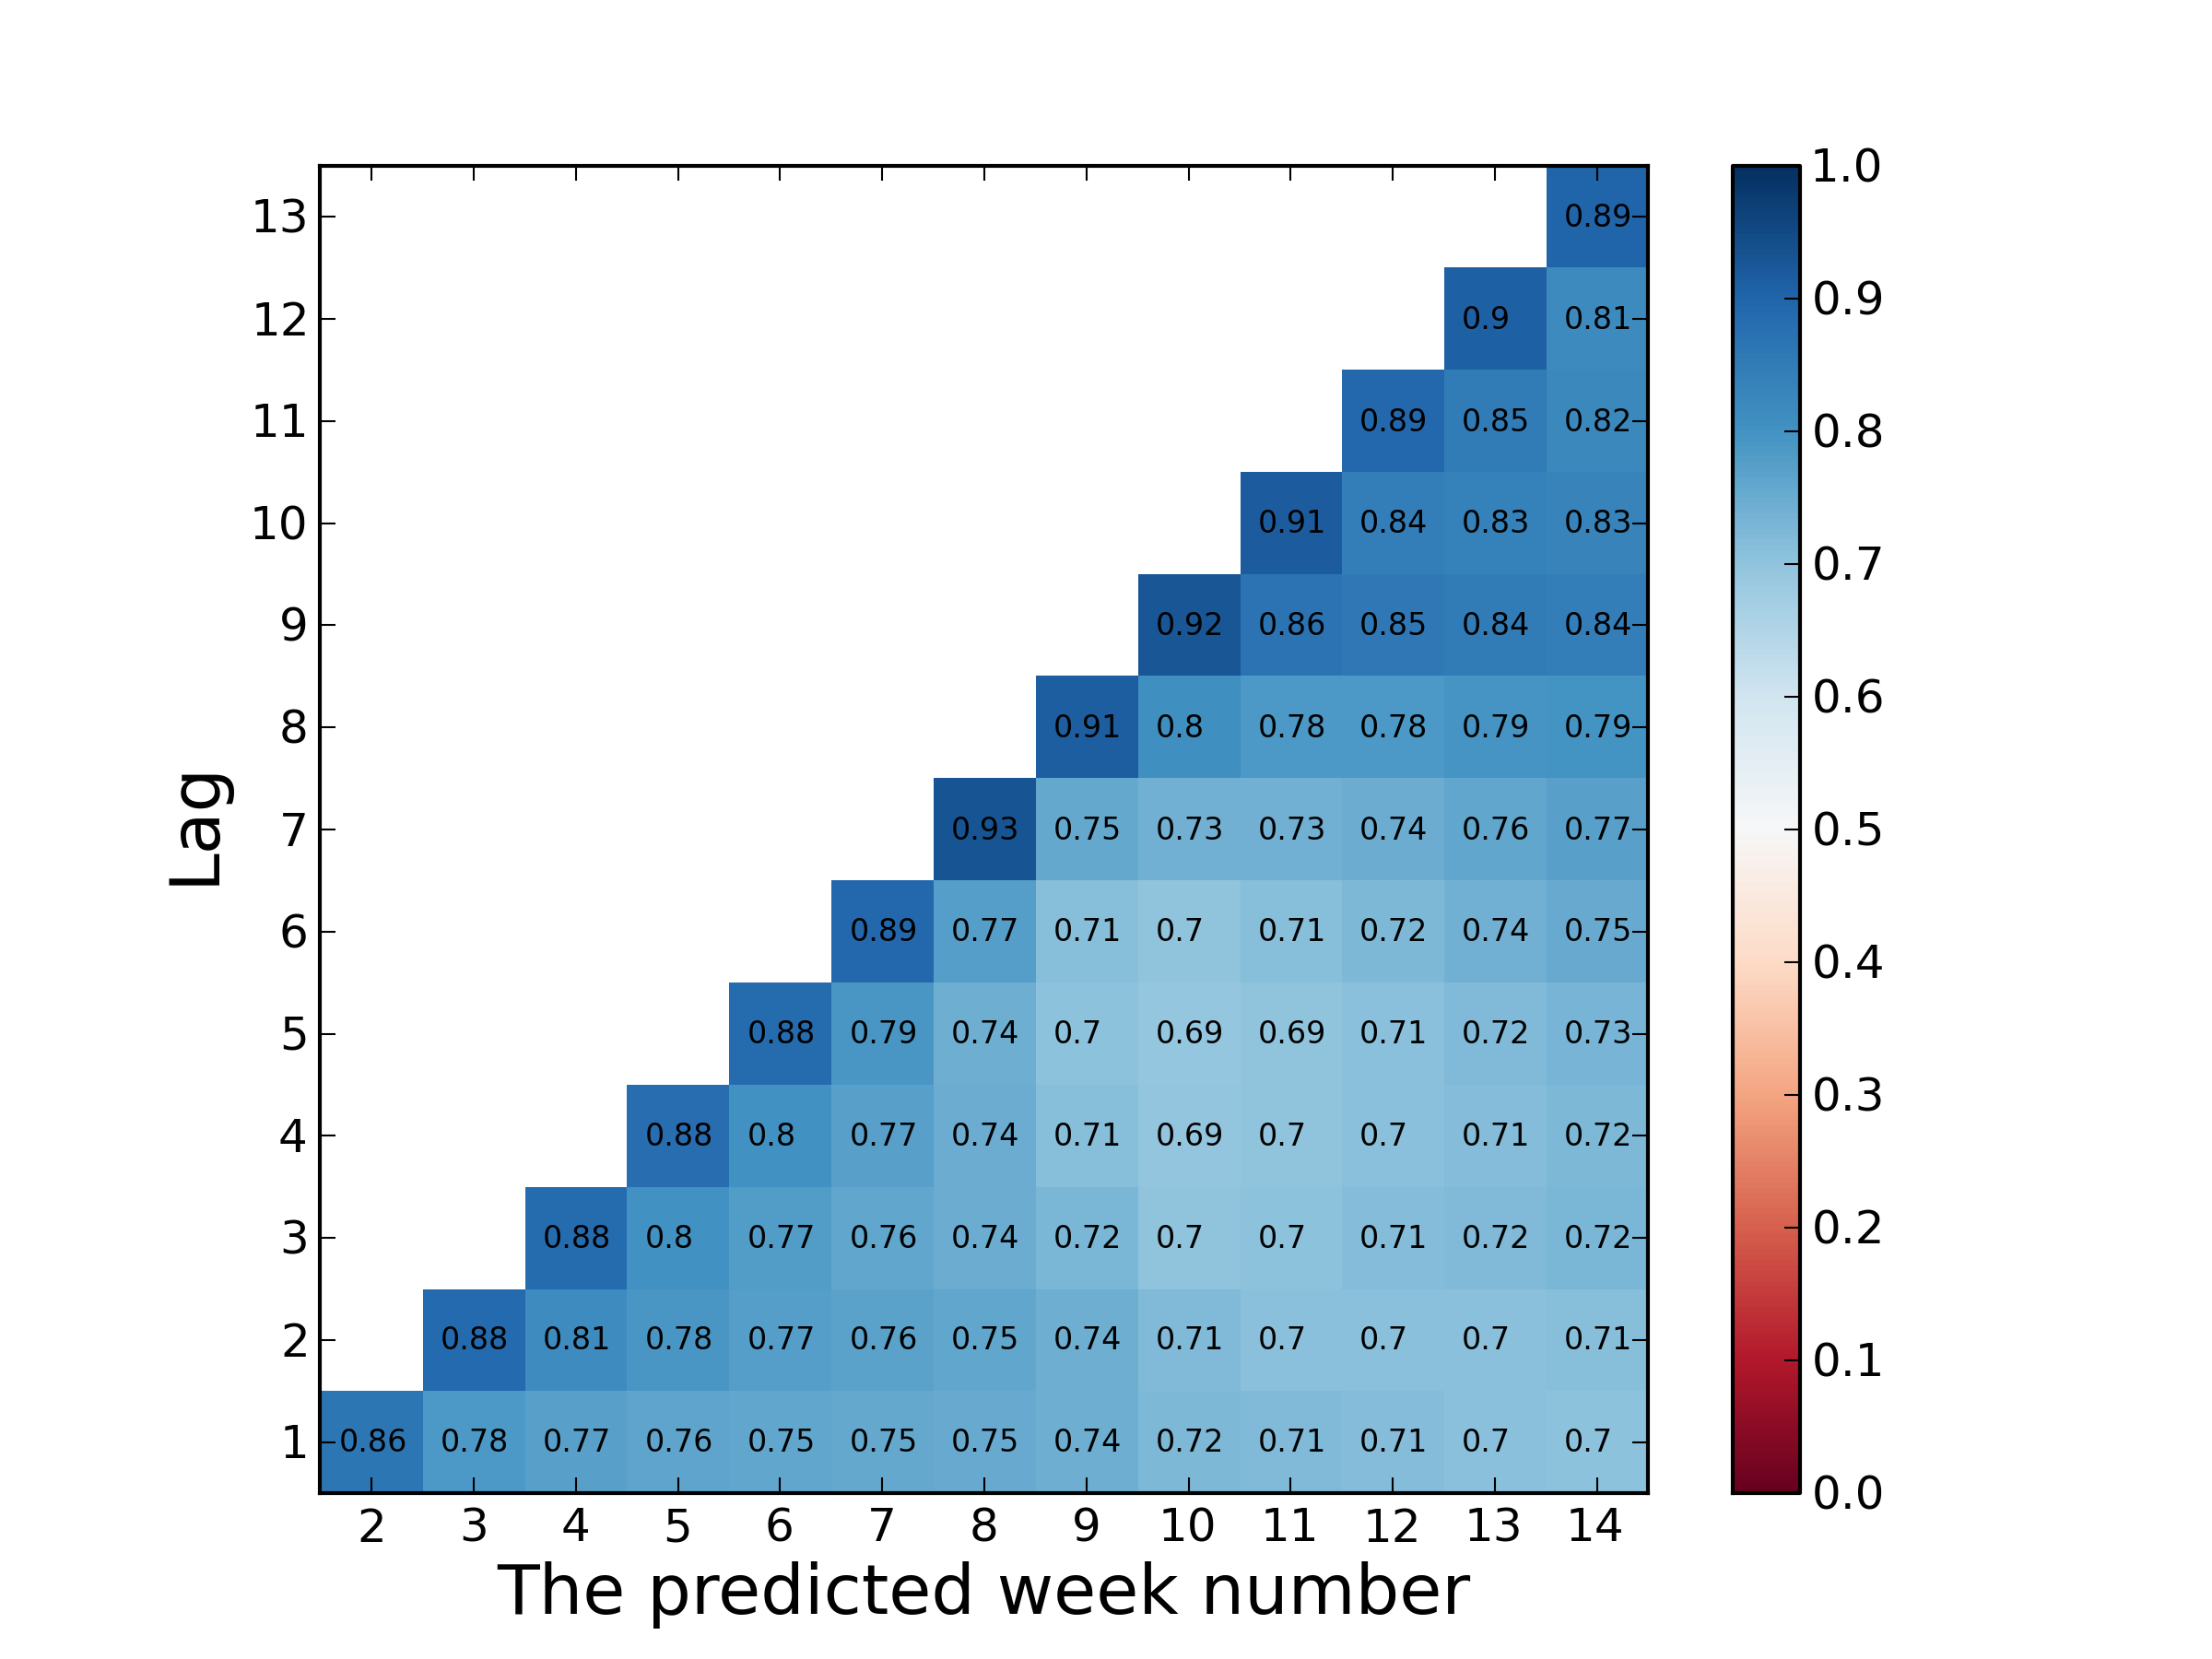
\includegraphics[width=1.0\textwidth]{figures/logreg/no_collab.png}
\end{figure}

\begin{figure}[ht!]
  \caption{Logistic regression results for the \forum cohort.}\label{fig:logistic_regression_heatmap_forum_only}
  \centering
    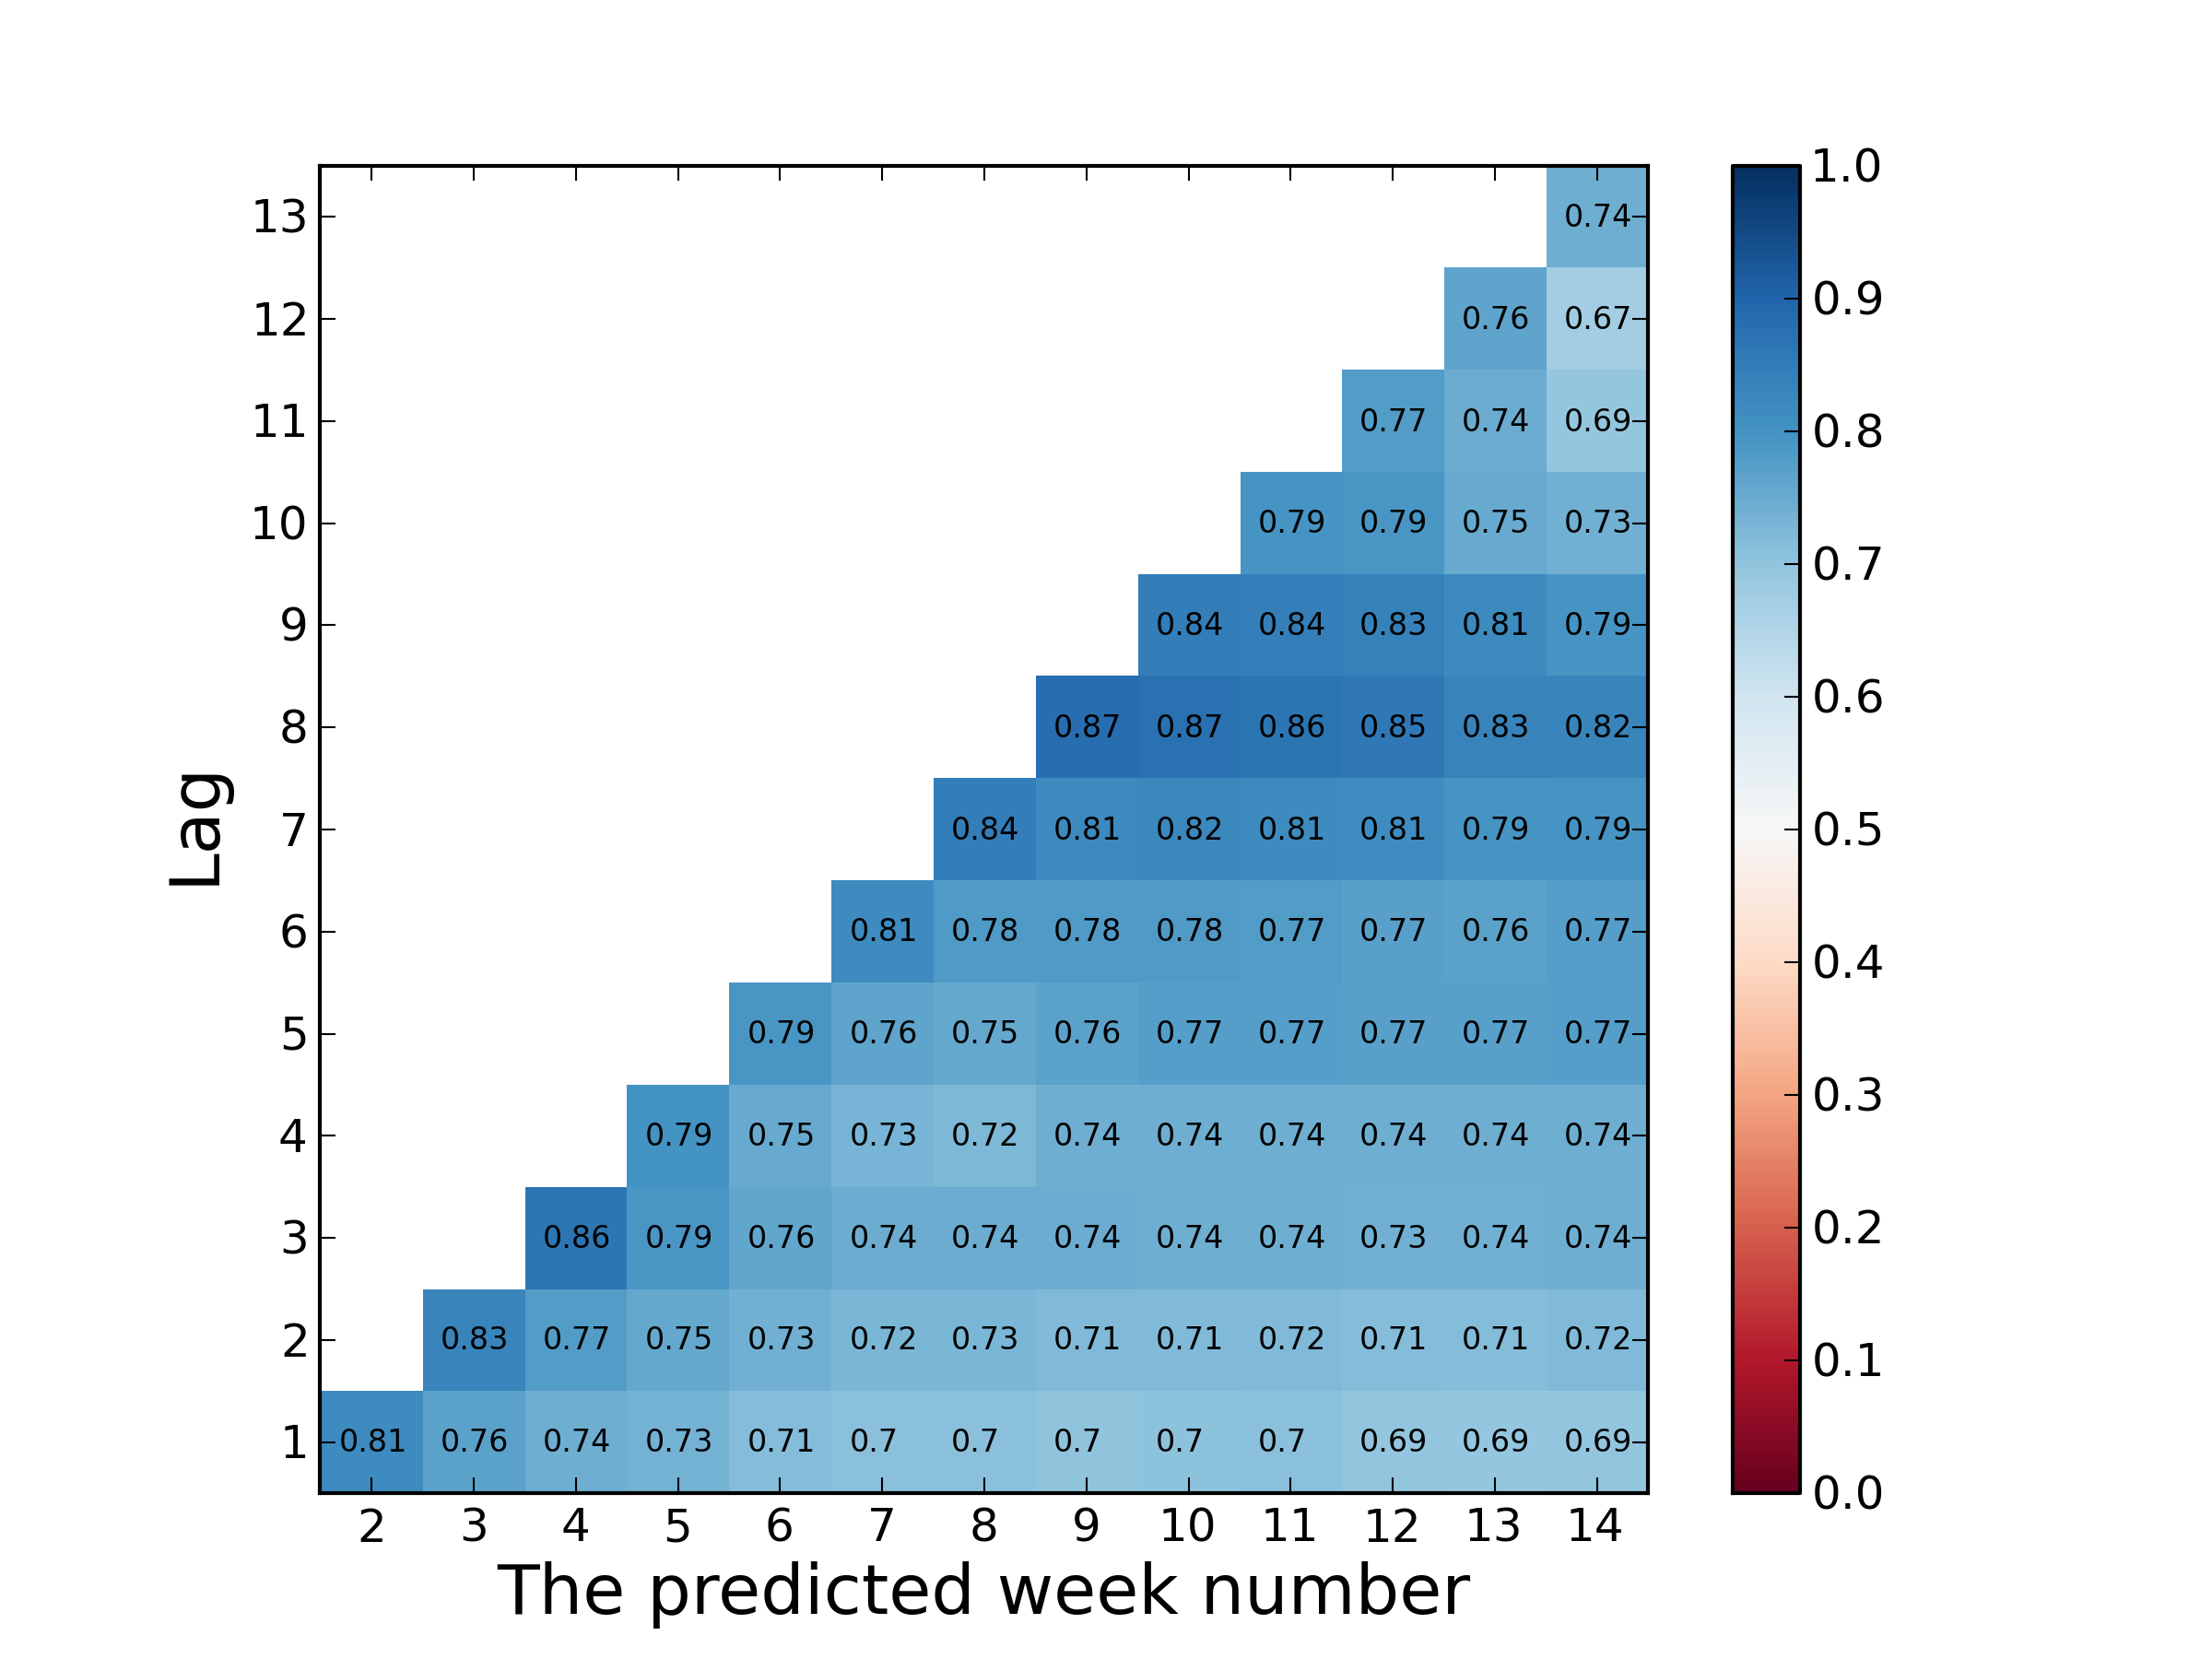
\includegraphics[width=1.0\textwidth]{figures/logreg/forum_only.png}
\end{figure}

\begin{figure}[ht!]
  \caption{Logistic regression results for the \both cohort.}\label{fig:logistic_regression_heatmap_forum_and_wiki}
  \centering
    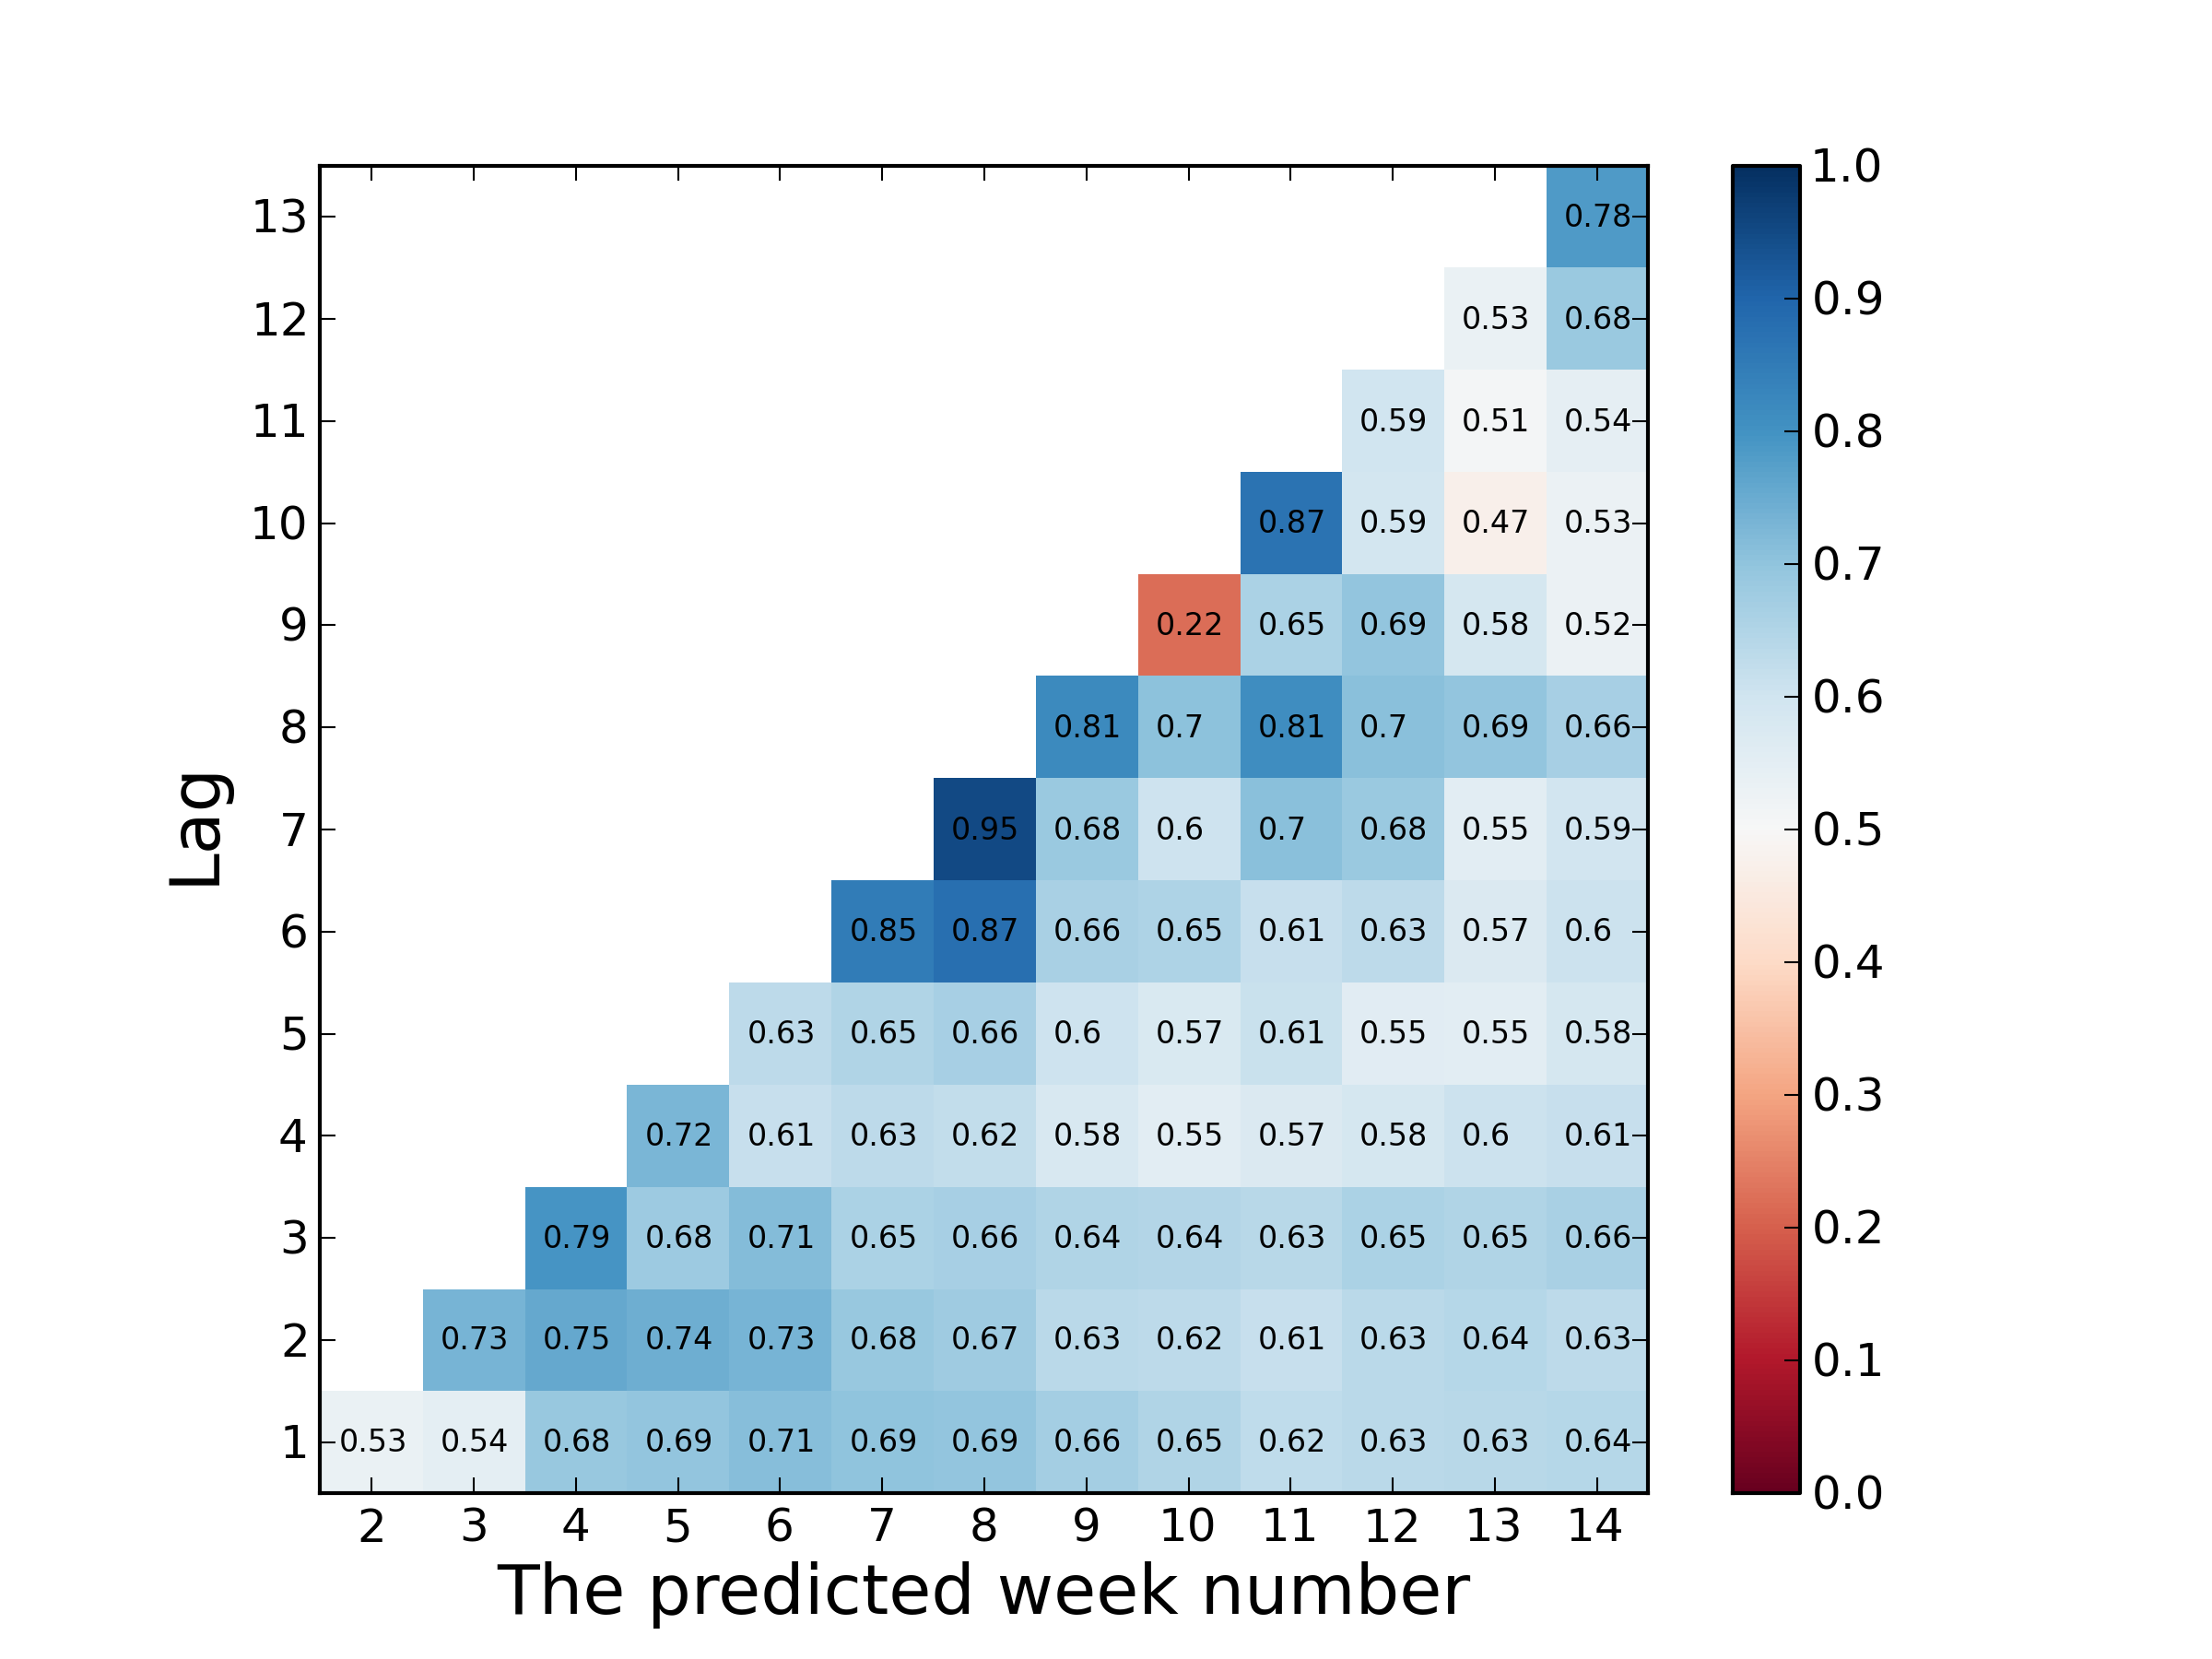
\includegraphics[width=1.0\textwidth]{figures/logreg/forum_and_wiki.png}
\end{figure}

\begin{figure}[ht!]
  \caption{Logistic regression results for the \wiki cohort.}\label{fig:logistic_regression_heatmap_wiki_only}
  \centering
    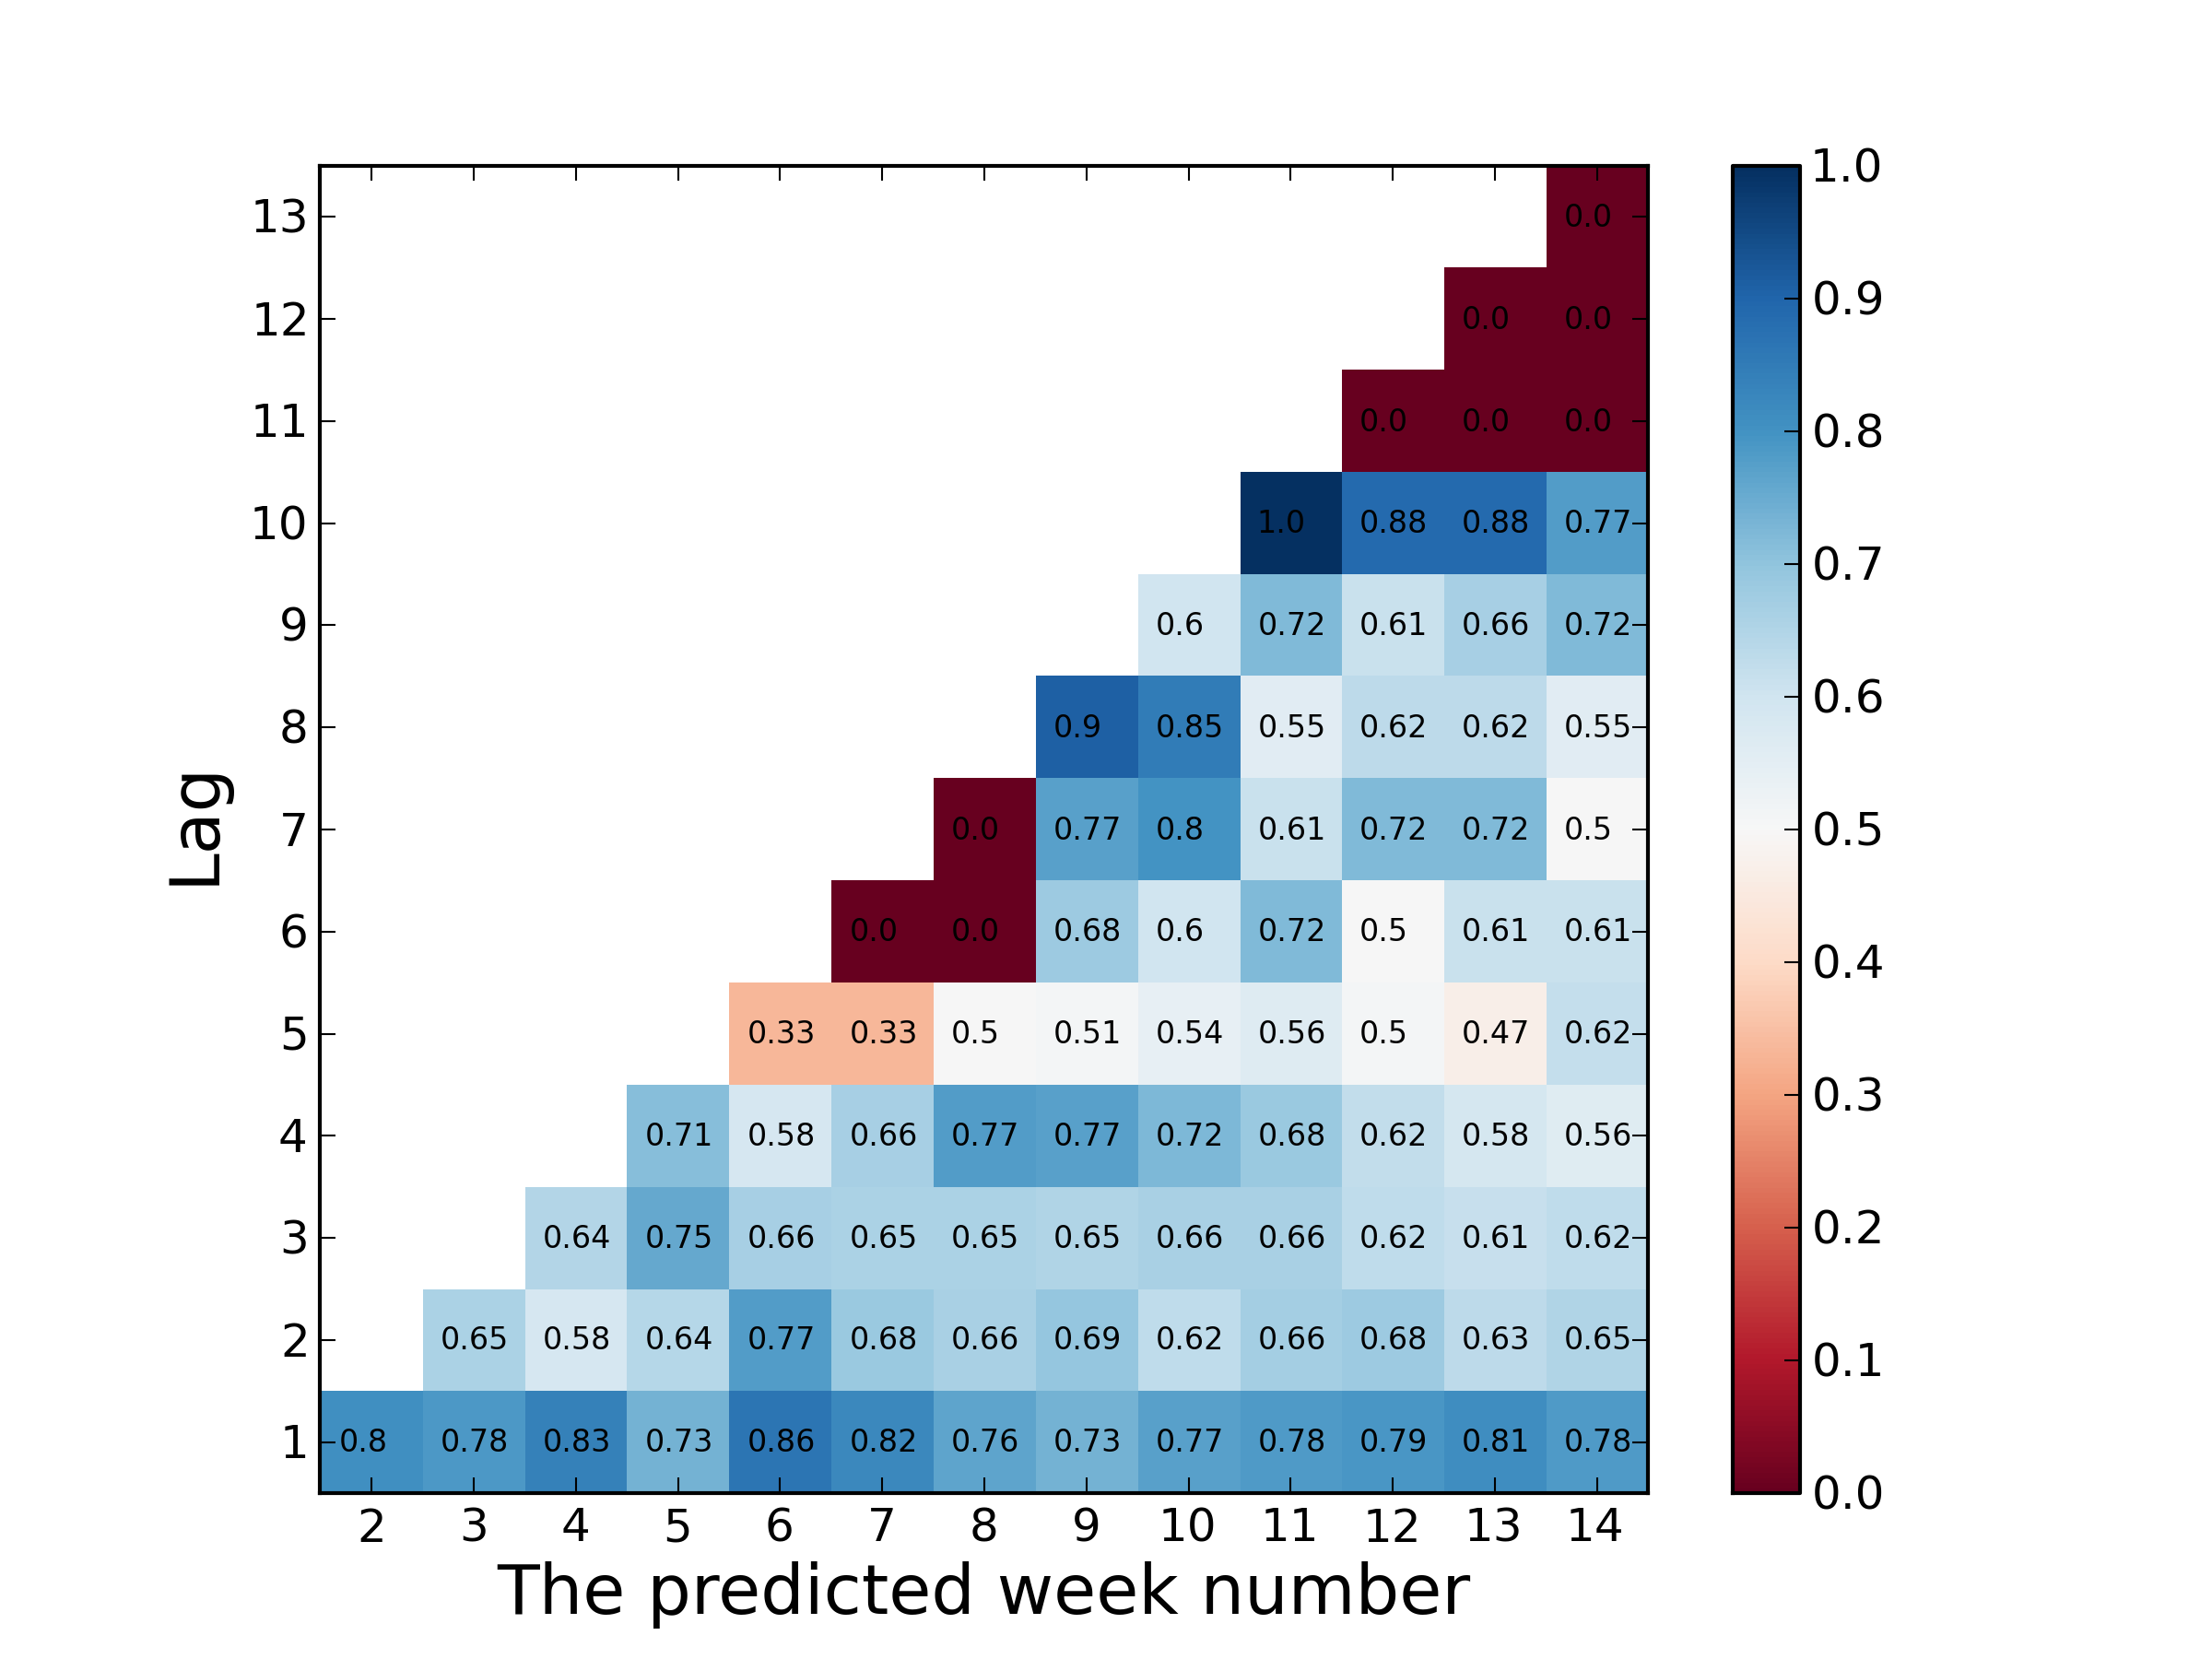
\includegraphics[width=1.0\textwidth]{figures/logreg/wiki_only.png}
\end{figure}

What follows is a deeper explanation of two interesting prediction problems and their results.

\paragraph{Are there early signs of stopout?}
One extremely interesting prediction problem is trying to predict student persistence into the last week of the course using a single week of data. Practically speaking, this would enable platform providers and instructors to predict which students would finish the course by the end of the first week. Potentially, this would allow instructors to interpret the reason for student stopout as motivational (such as just browsing) rather than course-specific reasons (such as the content becoming too difficult), because the students have not been exposed to much content yet. Furthermore, early-sign stopout prediction could allow courses to target certain types of students for some type of intervention or special content. If our models are successful, the results would imply that our extracted features are capturing a student's persistence far in advance. Remarkably across cohorts, the generated models achieved an AUC of at least 0.64, and reached as high as 0.78 in the case of the \wiki cohort. 

The \wiki AUC of 0.78, or even the \neither of 0.7 suggests it is possible to roughly estimate which students will finish the course. Implications include the ability to reach out to students likely to stop the course before they become disengaged, or giving a professor a rough indication of how many students to expect each week. If these predictions hold true for other courses, a prediction model could be used to measure the success of course experiments, such as changing course content.

In the case of the \wiki cohort, the model performed well for most later predictive weeks given a \lag of one. This indicates two things. Firstly, \wiki students show remarkably high early signs of persistence. Secondly, given more students, predictive models of the \wiki cohort would likely perform well. Owing largely to the small pool size of the \wiki cohort, model performance suffered, especially as \lag increased, because there were not enough students to appropriately train on. However, with a lead of one, the models used more student's data because we included all students who started in the course.

\paragraph{The prediction spike after the midterm}
Leading up to the midterm (in week 8), making predictions using a \lag of $i$, where $i$ is the current week, yields a fairly consistent AUC. In other words, students who will \sti after the midterm resemble their persistent counterparts up until week 8. However, using \lag 8 instead of 7, thereby including midterm data, produces an upward prediction spike in all four cohorts.

Perhaps the most striking spike example is in the most consistent cohort, the \neither students. If the model attempts to predict using a only lag 7, it realizes an AUC of 0.75. If the model expands to include midterm week data from week 8 and attempts to predict who will be in the course the next week, it achieves an AUC of 0.91! This is a significant spike. Similarly, the \both cohort increases AUC significantly from 0.68 in week 7 to 0.81 in week 8.

With the addition of the midterm week data the model is equipped to make reasonably consistent predictions through the end of the course. In fact, for the two cohorts of significant size, the region including and beyond week 8 achieves the highest AUCs of the entire course. This suggests that the midterm exam is a significant milestone for \sti prediction. It follows that most students who complete the midterm finish the course. For the two smaller cohorts, \wiki and \both, the region beyond week 8 realizes terrible predictive power because too few students remain in the course to accurately train on.

\section{Randomized Logistic Regression}
Another use of logistic regression is to assess the importance of features. Our model analyzes 27 features to model \sti. In order to best fit a training set, the model optimizes weights for each feature (outlined in the logistic regression section). By weighting the features we gain a sense of how predictive each feature is. However, the logistic regression model misses the mark if two variables are highly predictive, yet very correlated, because it will only select one. The unselected feature will appear to have a low coefficient. To work around single feature selection we perform Randomized logistic regression which works as follows: 

\begin{description}
\item {Step 1:} Sample without replacement  75\% of the training data each time. 

\item {Step 2:} Train a logistic regression model on the sub-sampled data (with regularization).

\item {Step 3:} For every feature evaluate $b_s^{i}=\mu(w_i,th)$ where $\mu$ is a unit step function and $w_i$ is the \coeff for \co $i$ and $th$ is the threshold we set to deem the feature important. This is set at 0.25. 

\item {Step 4:} Repeat Steps 1, 2 and 3 a total of 200 times. 

\item {Step 5:} Estimate the importance of the \co $i$ by $\sum_s b_s^{i}$. 

\end{description}

We applied \rLR logistic regression to the \sti prediction problem using the exact same process as we did in logistic regression (e.g. flattening a feature set using lead and \lag values etc.) This technique is also referred to as stability selection \cite{meinshausen2010stability}.


\subsection{Experimental setup}
We ran randomized logistic regression for every lead, \lag and cohort combination. For each experiment, randomized logistic regression resulted in a vector of \cov weights. Each weight ranged from 0 to 1.
\footnote{We used the scikit-learn Randomized Logistic Regression implementation.}

\subsection{Experimental results}
Randomized logistic regression analysis gave us fascinating covariate weight vectors for all 91 experiments and all cohorts. For each experiment the randomized logistic regression gives us weights for all the \cov which are student features for different weeks.  In order to gain a more quantitative grasp of which features matter, as well as which week's data mattered for different prediction problem, we performed two different types of aggregations. 

\begin{paragraph}
{Week invariant feature importance} To calculate the importance of a feature, we first evaluate its importance in each of the 91 experiments. We sum the weights associated with it across different weeks, then divide it with the sum of all weights for that experiment. This gives its weight relative to every other feature in that particular experiment. We illustrate this procedure for evaluating feature 1's importance in an experiment where the lag=3 in Figure~\ref{fig:wif}. After quantifying importance for the feature of each experiment, we average the number to get the week-invariant feature importance.  Figures \ref{fig:randomized_logistic_regression_no_collab} to \ref{fig:randomized_logistic_regression_wiki_only} summarize these normalized average feature weights. 

\begin{figure}[ht!]
  \caption{Aggregating feature 1's weights to assemble relative feature importance for a single experiment. In this example, the lag is 3. Three weeks data is used to predict a \sti in a future week. The Randomized logistic regression gives the weights for all 27 features for all three weeks (unnormalized). To assemble the week invariance relative weight for feature 1 we sum the weights and divide it with the total weights. We note that this is a heuristic. }\label{fig:wif}
  \centering
    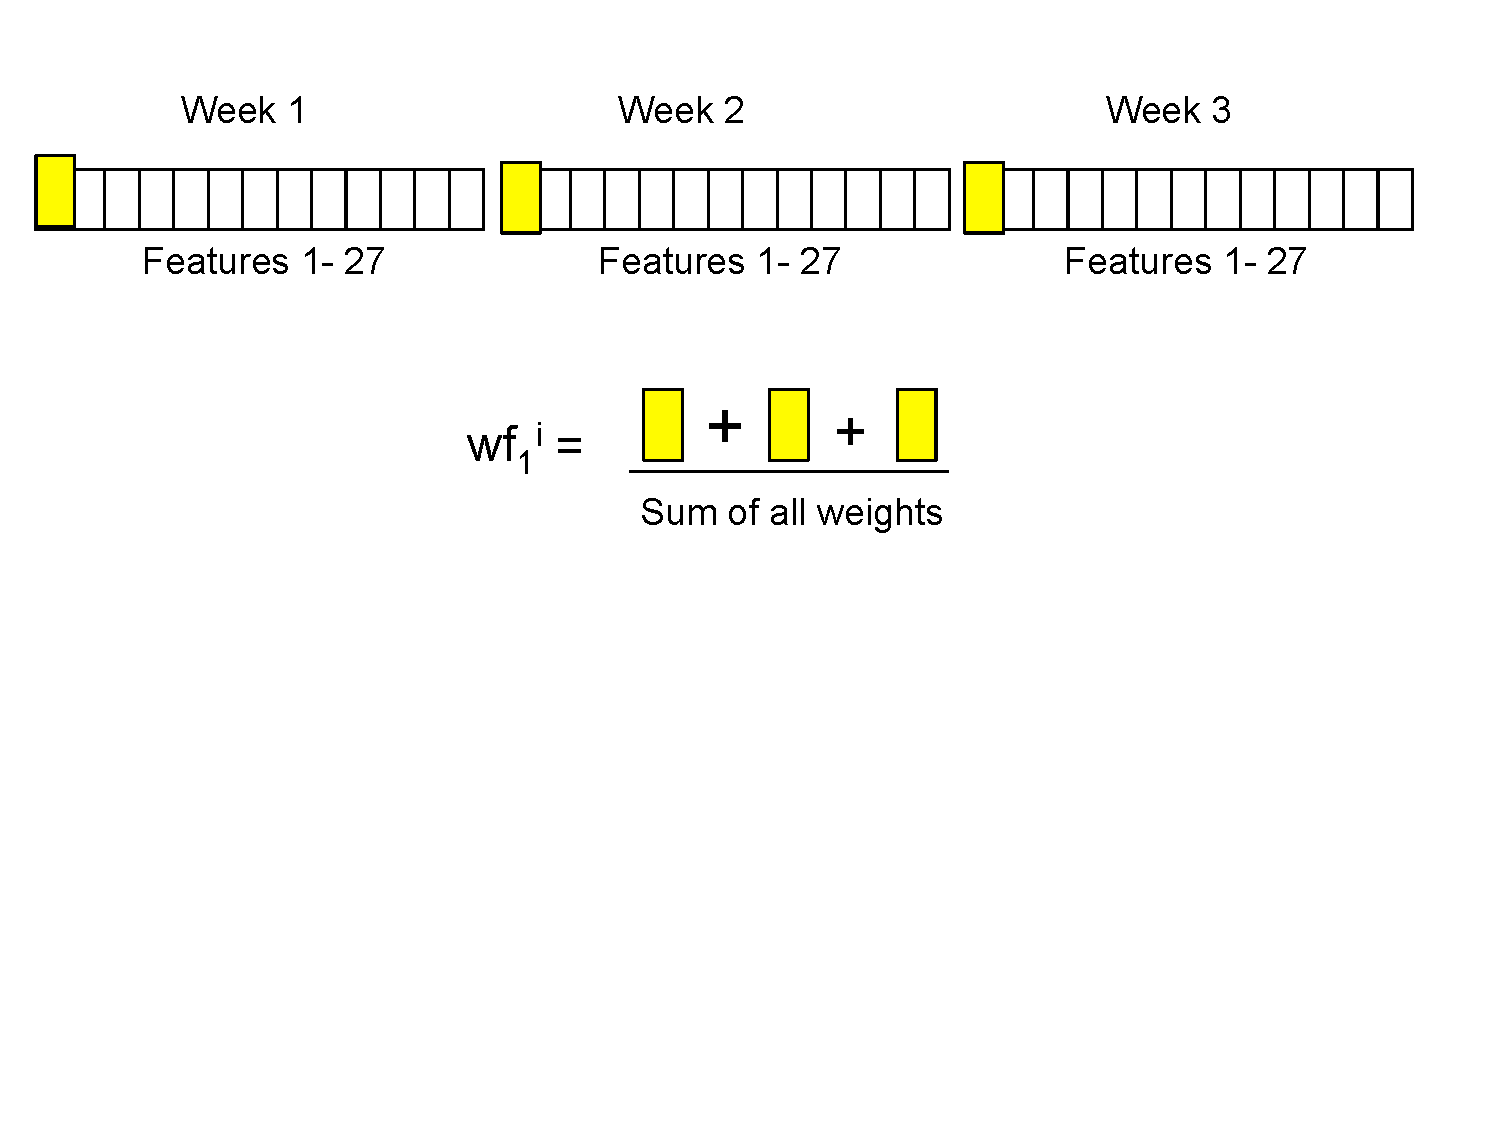
\includegraphics[width=0.6\textwidth]{figures/wif}
\end{figure}

\begin{figure}[ht!]
  \caption{Feature importances for the \neither cohort.}\label{fig:randomized_logistic_regression_no_collab}
  \centering
    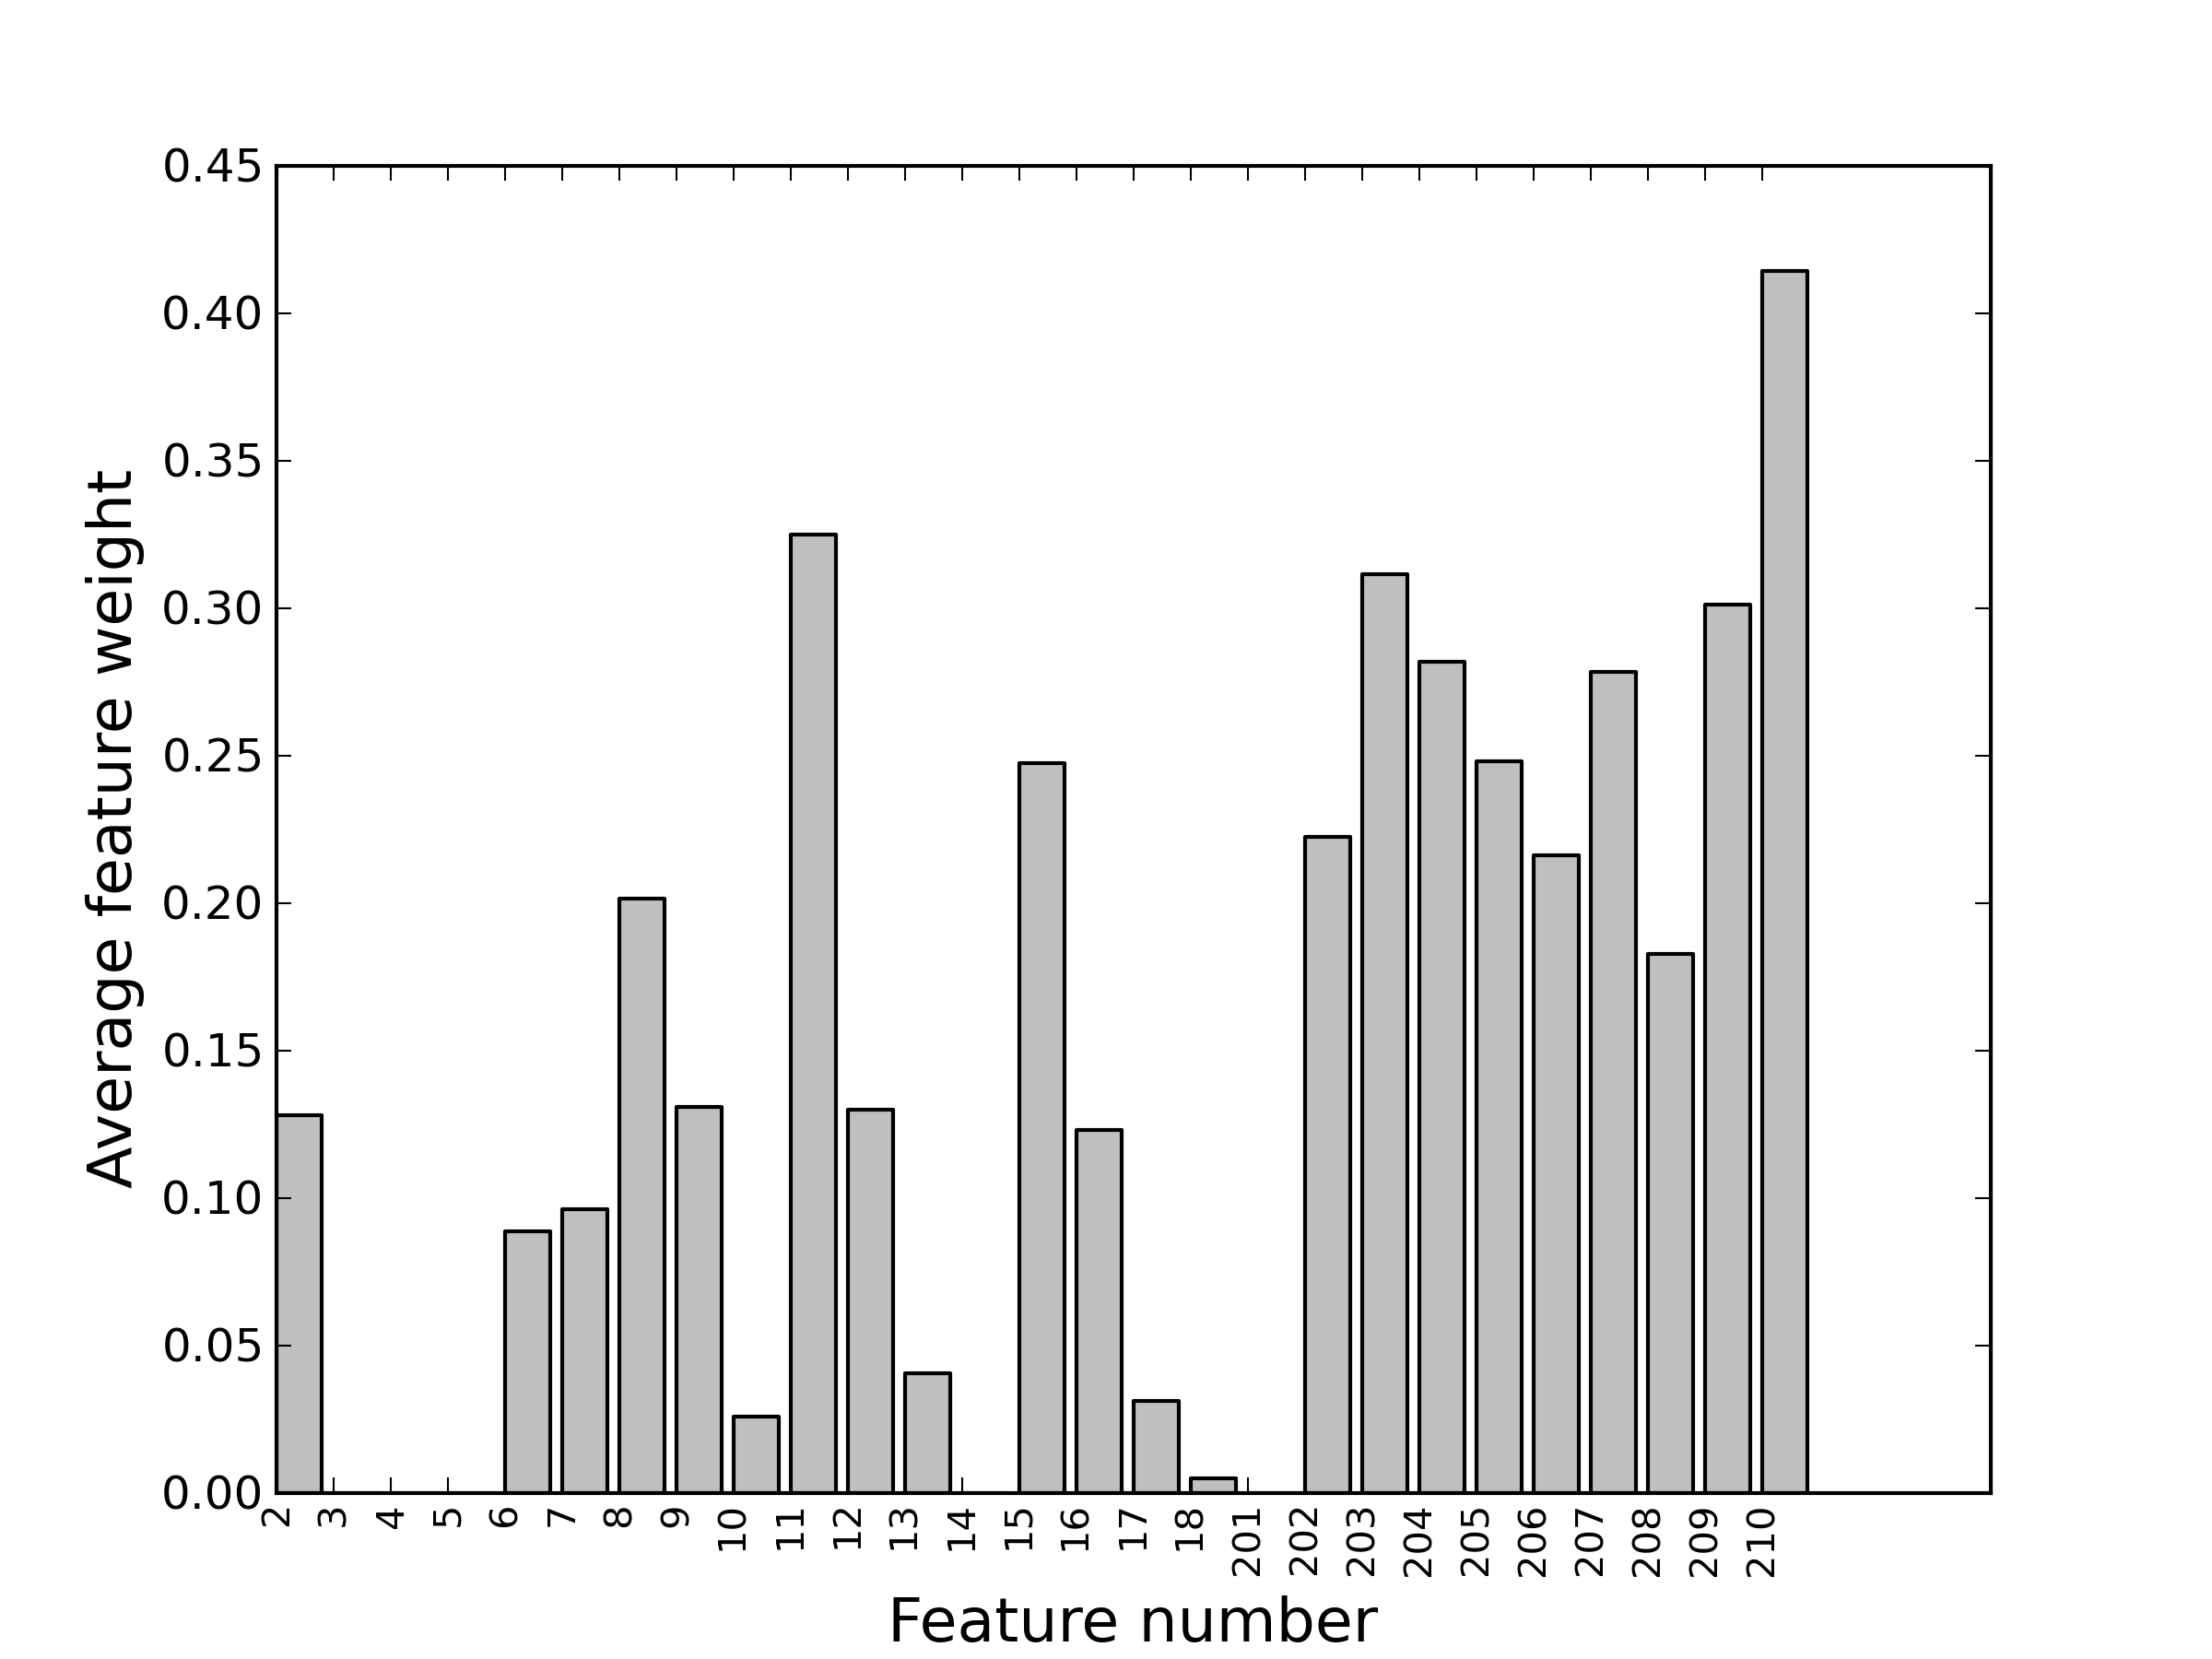
\includegraphics[width=0.7\textwidth]{figures/logreg/randomized_no_collab.png}
\end{figure}

The first thing that struck us as we looked at these plots was the difference in feature weights between the self-proposed features and the crowd-proposed features. In all four cohorts, the majority of the weight lies in the crowd-proposed features \ref{section:crowdself} (\x{201} through \x{210})! Clearly, the crowd can be utilized to a great degree. As features mostly represent high level constructs, such as the percentiles (\x{202} and \x{203}), these plots suggest that those types of features have a very high predictive power. Additionally, they mostly involve the submissions table in MOOCdb. This includes the lab grade (\x{206}), pset grade (\x{207}) and predeadline submission time (\x{210})).

In the \neither cohort, the feature most indicative of \sti is the average predeadline submission time. The \forum cohort looks very similar, but uses a broader spectrum of features. In particular, we see that \x{5}, the average length of forum posts, is also highly predictive (of course, this could not have shown up in the \neither cohort, as by definition those students do not participate in the forum). Interestingly, we see a very low predictive power from the number of forum posts(\x{3}) and the number of forum replies (\x{201}), despite the fact that the length of the forum post is very important. This could imply that longer posts are indicative of more engagement in the course, or a greater mastery of the material.

\begin{figure}[ht!]
  \caption{Feature importances for the \forum cohort.}\label{fig:randomized_logistic_regression_forum_only}
  \centering
    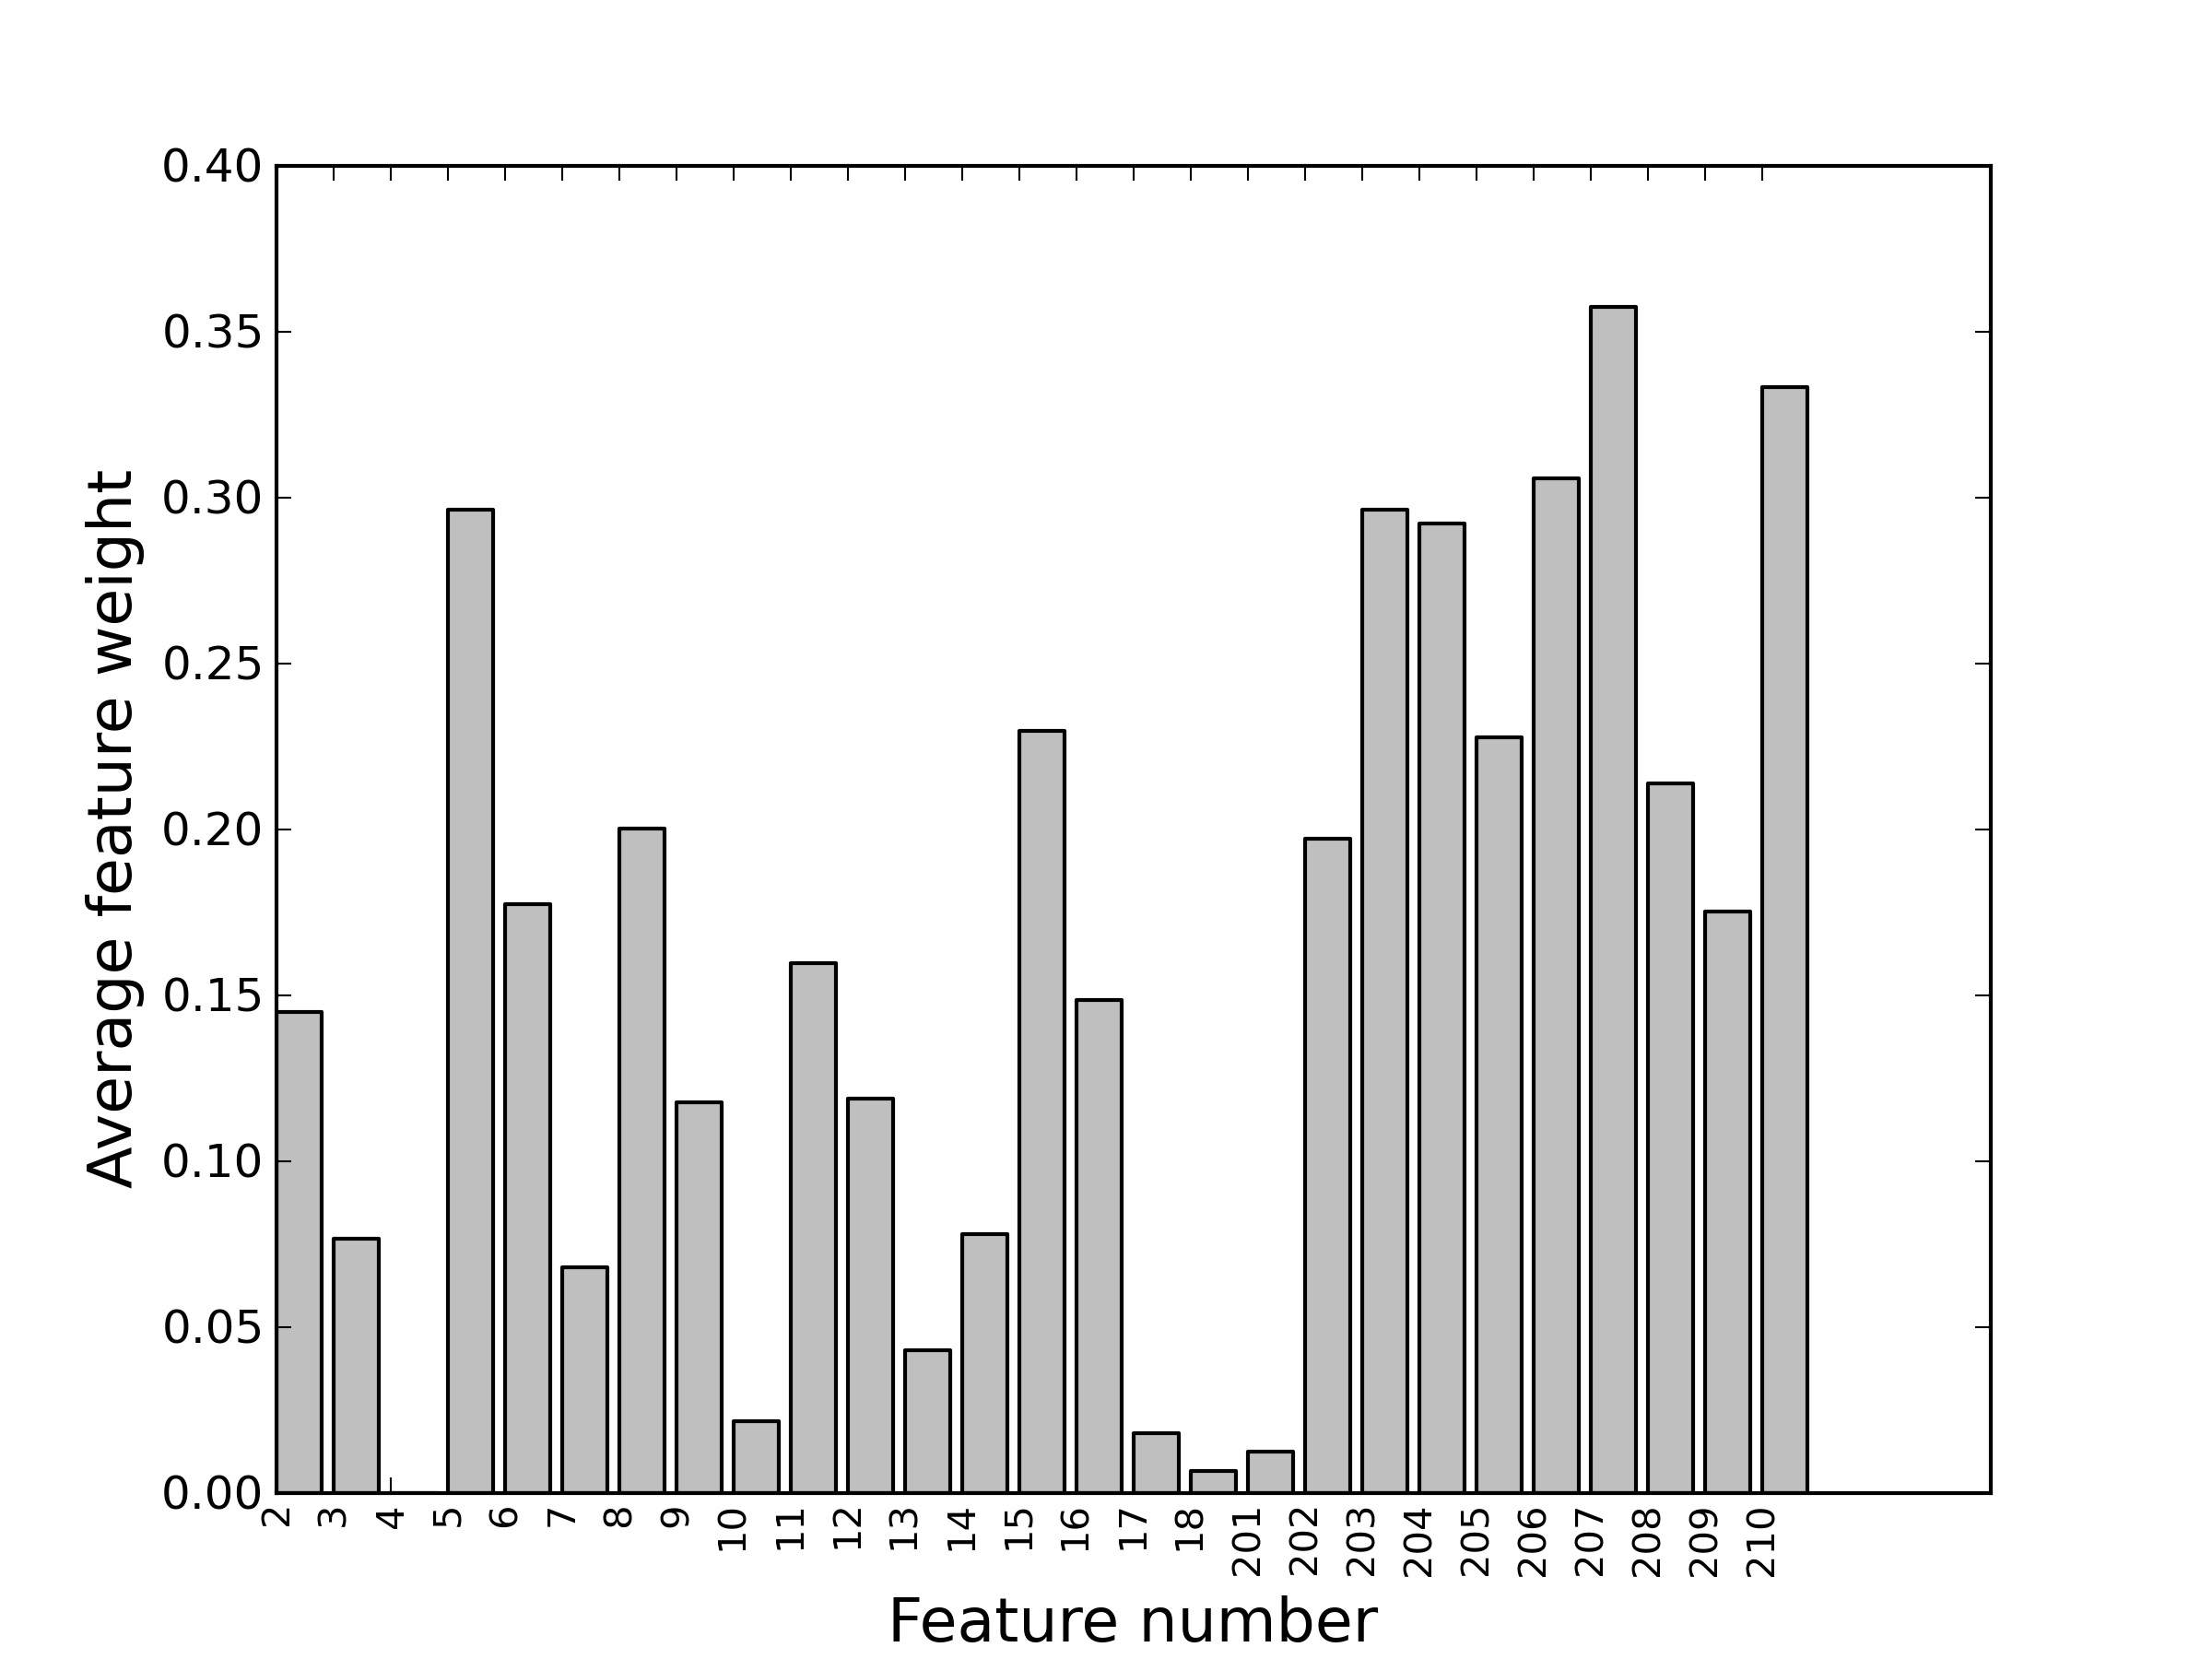
\includegraphics[width=0.7\textwidth]{figures/logreg/randomized_forum_only.png}
\end{figure}

In the both of our smaller cohorts, \both and \wiki, the lab grade (\x{206}) and lab grade over time (\x{207}) are the most predictive features. Although both of these cohorts participated in the Wiki, the number of Wiki edits (\x{4}) actually contains insignificantly small predictive power in both cases. Both cohorts show similar distributions overall. Similar to the larger cohorts, features related to submissions hold the most predictive power.

\begin{figure}[ht!]
  \caption{Feature importances for the \both cohort.}\label{fig:randomized_logistic_regression_forum_and_wiki}
  \centering
    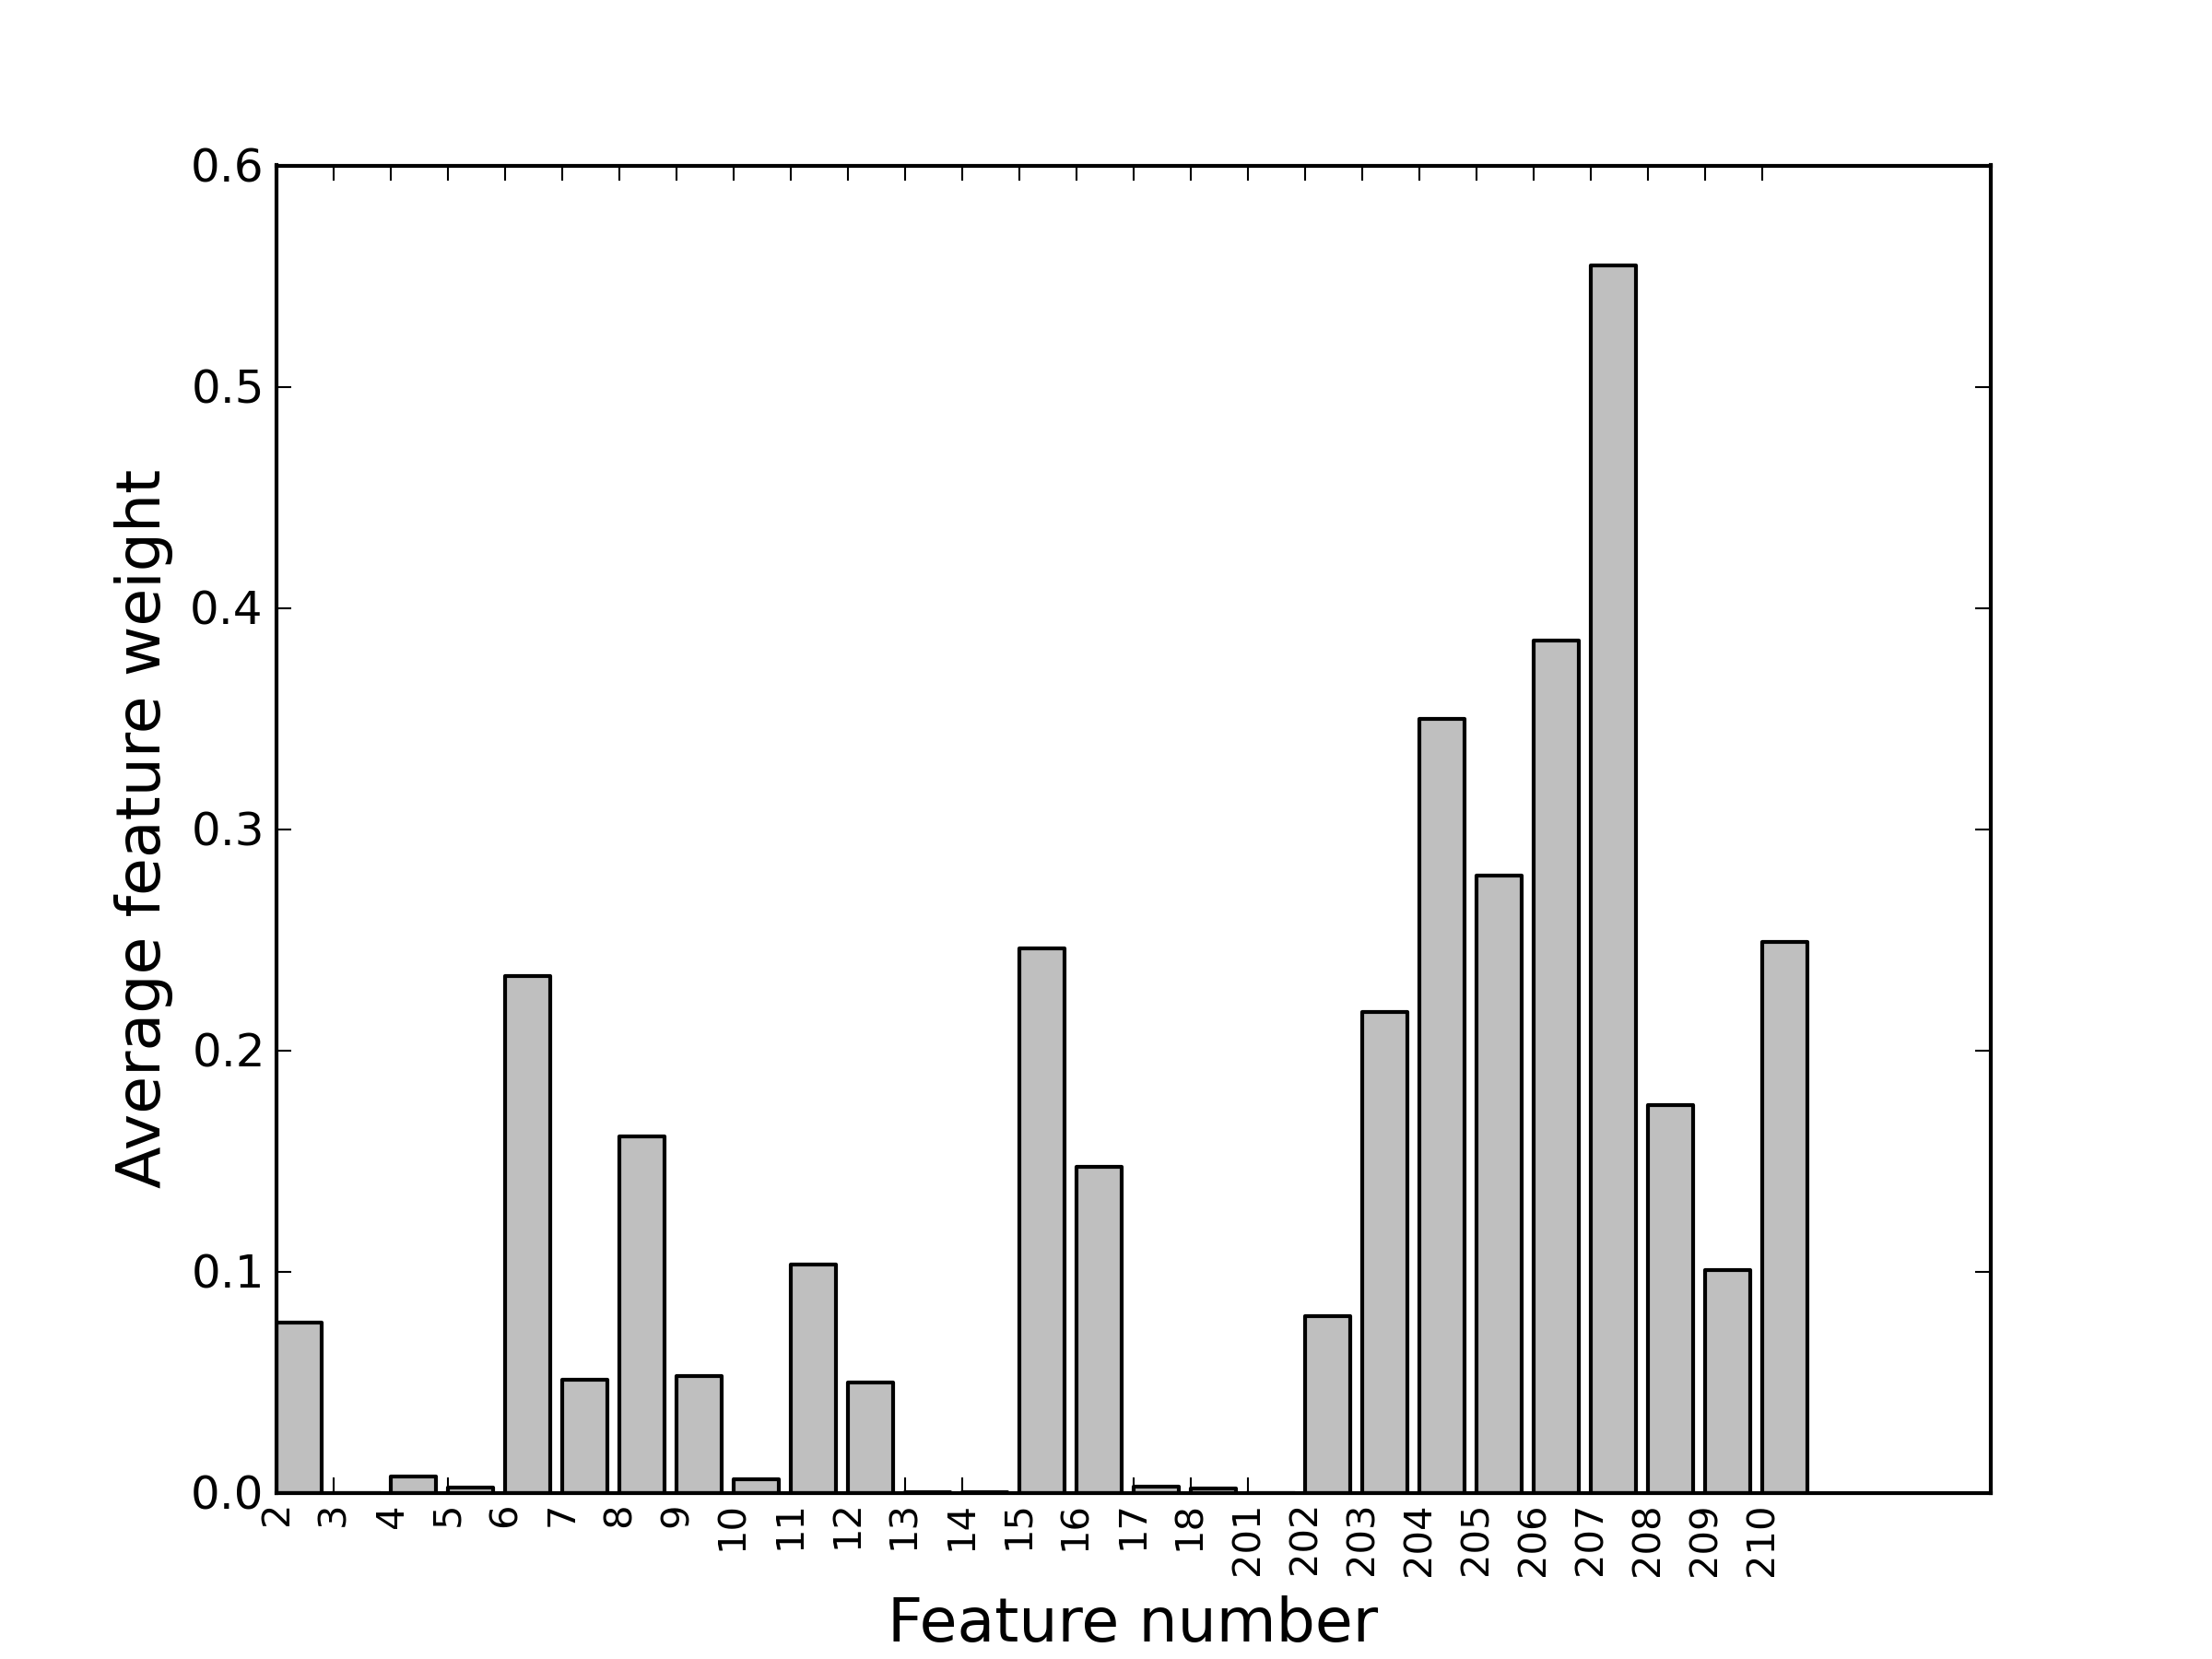
\includegraphics[width=0.7\textwidth]{figures/logreg/randomized_forum_and_wiki.png}
\end{figure}

\begin{figure}[ht!]
  \caption{Feature importances for the \wiki cohort.}\label{fig:randomized_logistic_regression_wiki_only}
  \centering
    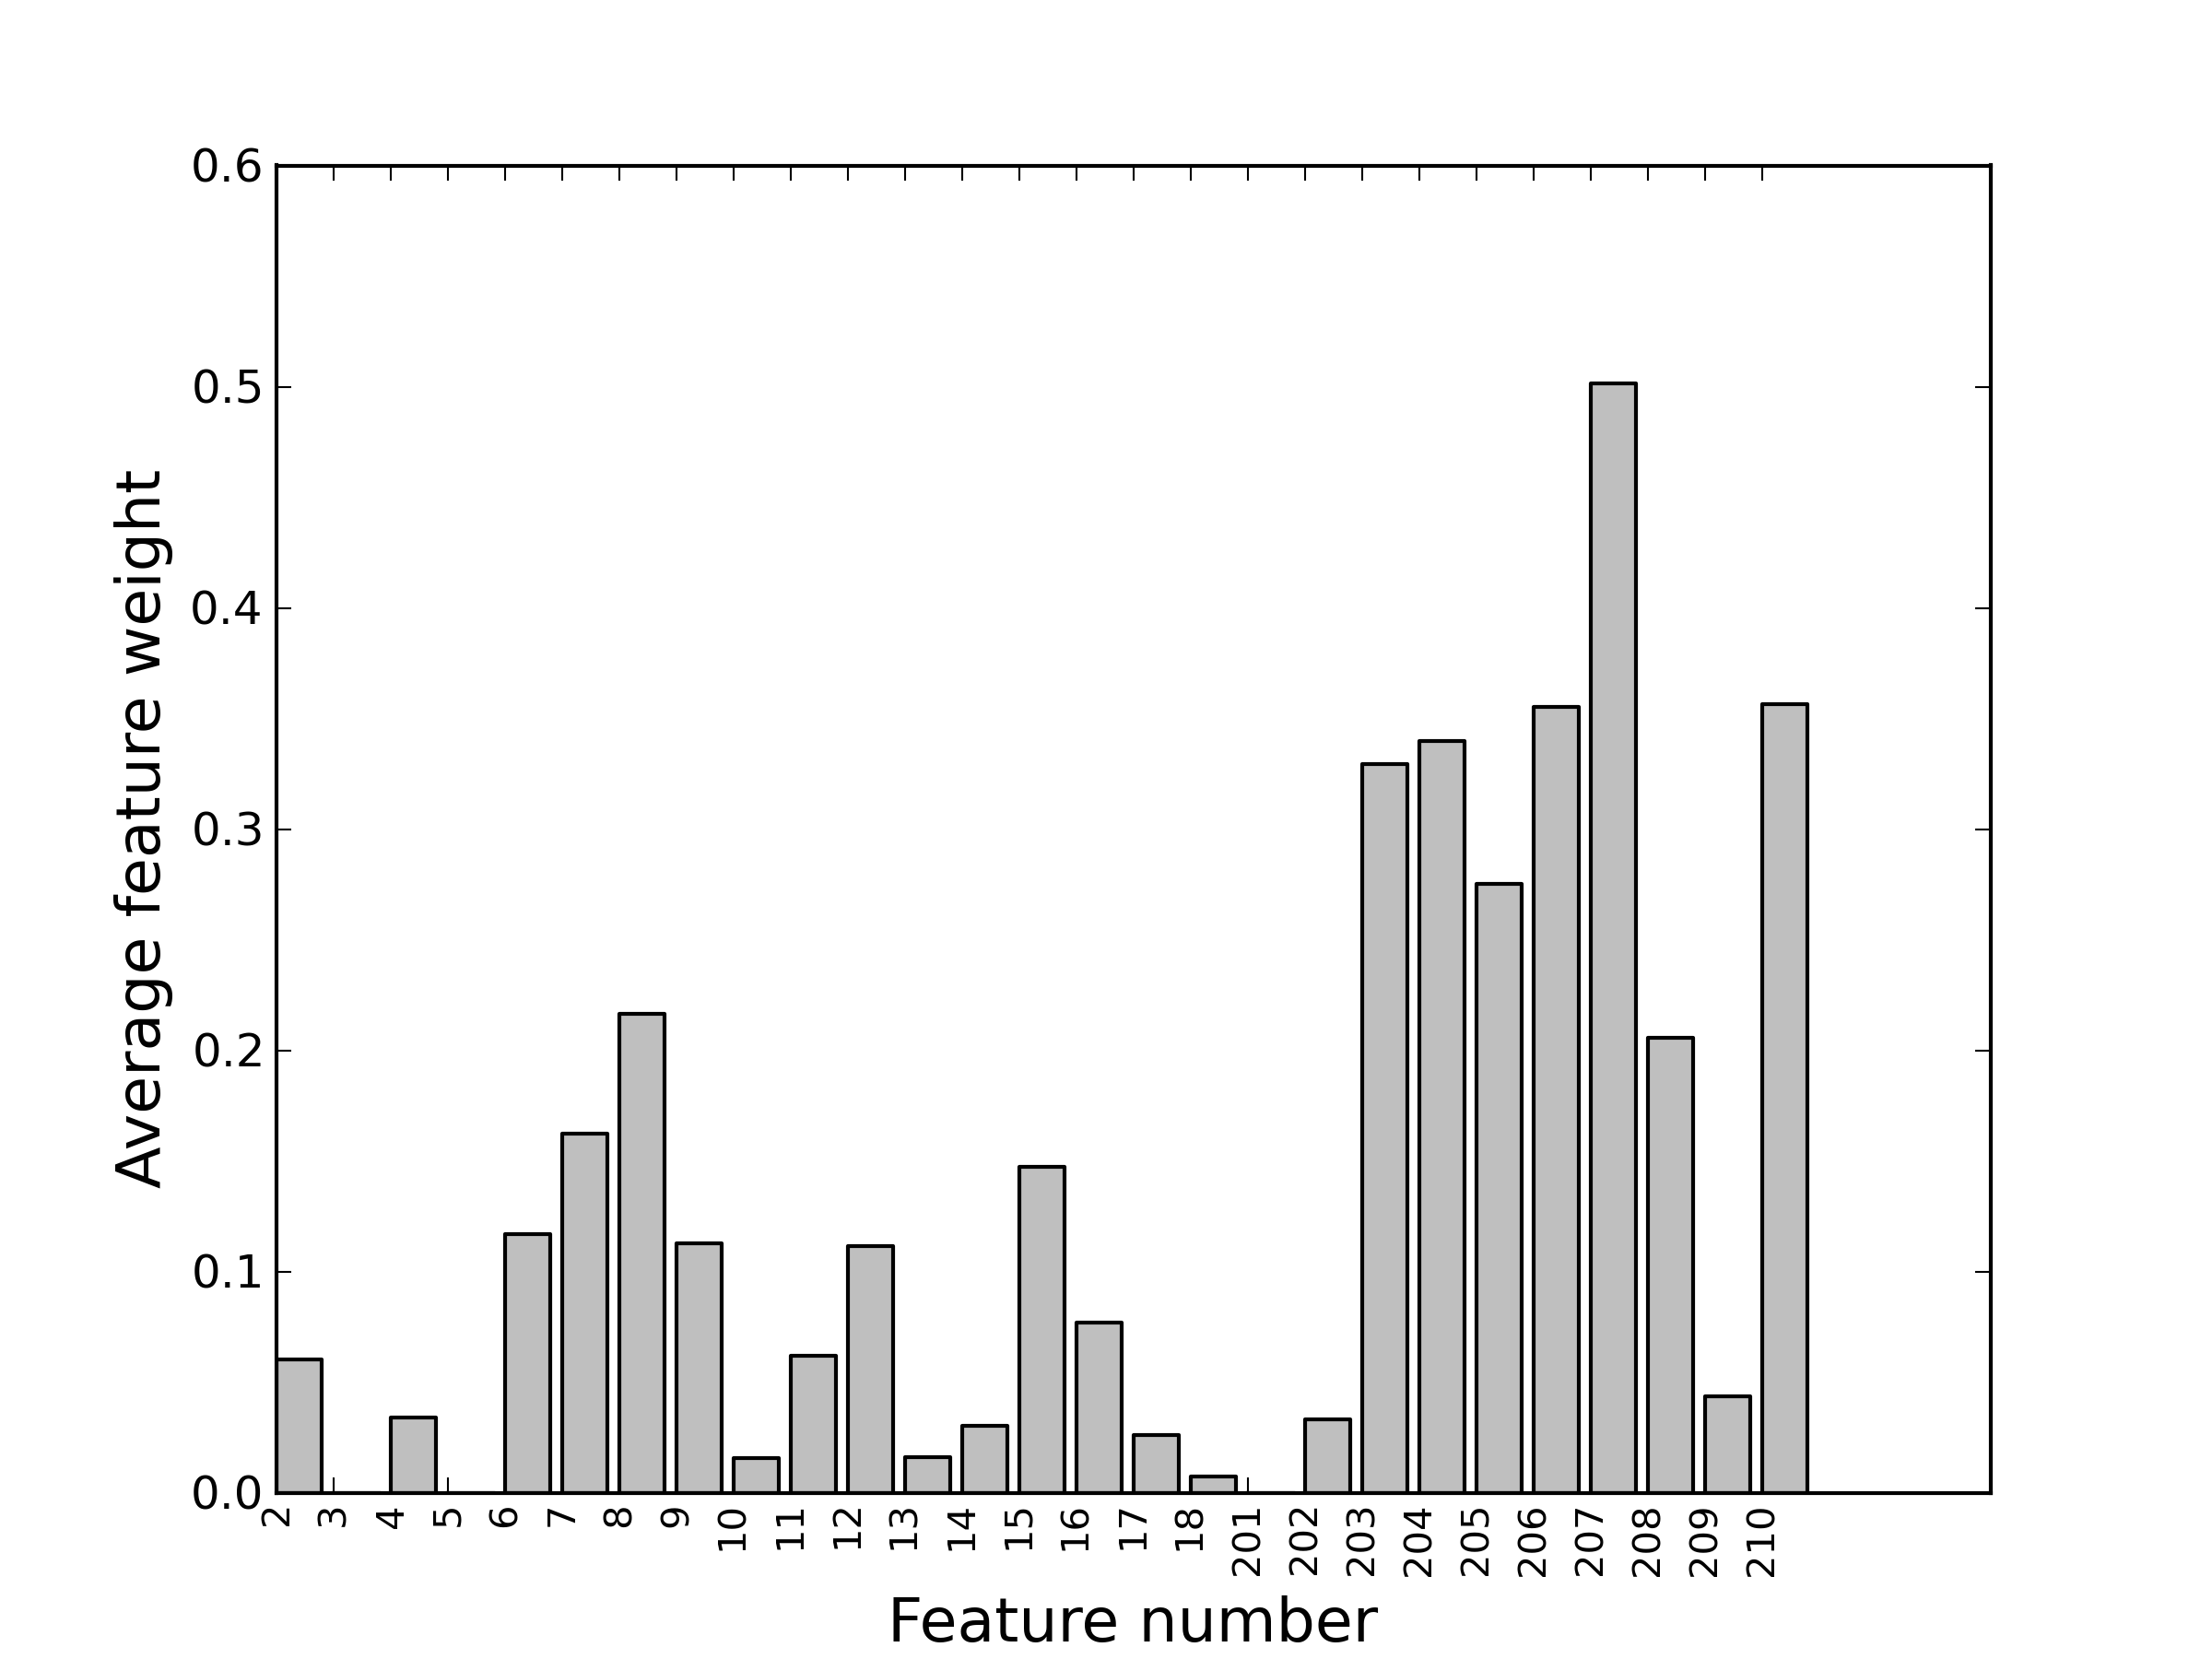
\includegraphics[width=0.7\textwidth]{figures/logreg/randomized_wiki_only.png}
\end{figure}

\end{paragraph}

\begin{paragraph}
{Feature invariant week importance} For any given lag (that is data from weeks 1-to-lag) we wanted to assess which of the week's features (data) are important for a prediction problem. We call this feature-invariant week importance. To evaluate this, we first group the experiments by lag, then for each experiment aggregate the weights for features for each week. We then normalized this value with the total sum of weights. This provided us the relative normalized importance of that week in that experiment. We illustrate this process in Figure~\ref{fig:fiw}. We then repeat this for all the experiments with the same lag and then sum the normalized importances for a week and plot this sum for each lag in the heatmap as shown in the Figure~\ref{fig:randomized_over_time_no_collab}. 

\begin{figure}[ht!]
  \caption{Aggregating different weeks weights to assemble weeks relative importance for a single experiment for a given lag. In this example, the lag is 3. That is,  three weeks data is used to predict a \sti in a future week. The Randomized logistic regression gives the weights for all 27 features for all three weeks (unnormalized). To assemble the feature-invariant relative weight for week 1 we sum the weights for all features in week 1 and divide it with the total weights. We note that this is a heuristic. }\label{fig:fiw}
  \centering
    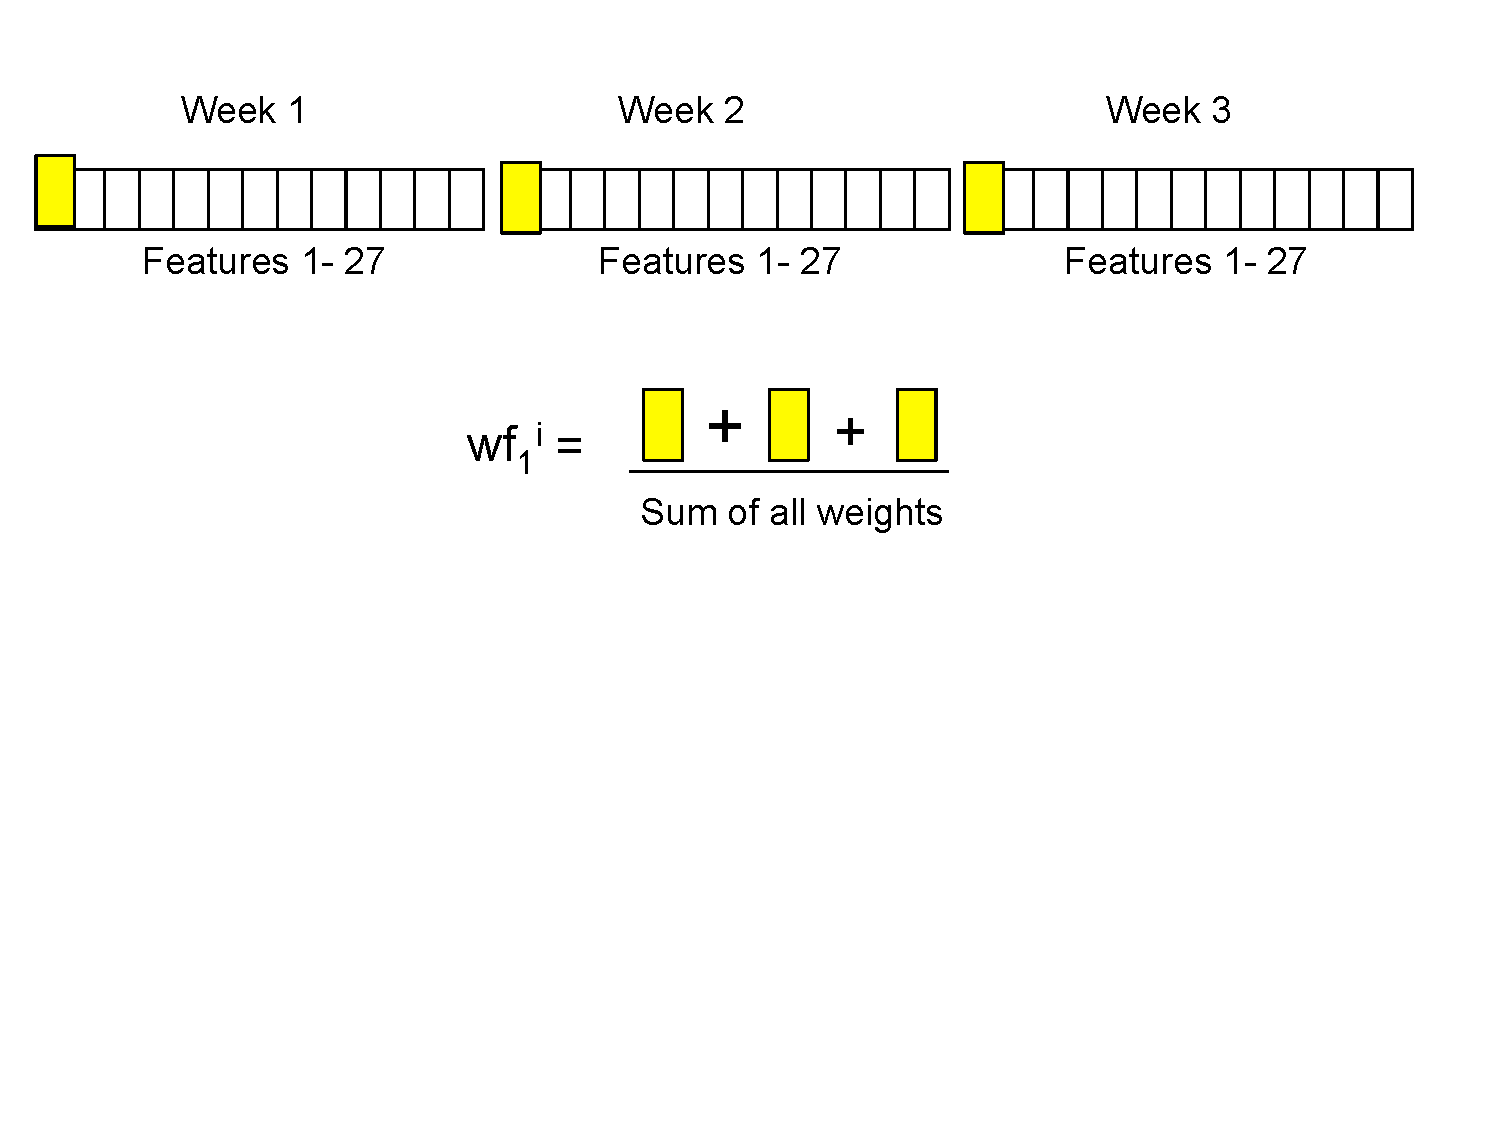
\includegraphics[width=0.6\textwidth]{figures/wif}
\end{figure}


As might be expected, most feature vectors used only more recent weeks of data in order to predict. For example, for the \neither cohort, for a \lag of 8, predicted week of 11, the majority of the first 6 weeks of data have no feature weight, and the nonzero weights are all below 0.15, whereas features of week 10 include weights as large as 0.965 (for \x{11}). Figures \ref{fig:randomized_over_time_no_collab} through \ref{fig:randomized_over_time_wiki_only} show a heatmap of these results.

\begin{figure}[ht!]
  \caption{Feature week's importance as \lag varies for the \neither cohort.}\label{fig:randomized_over_time_no_collab}
  \centering
    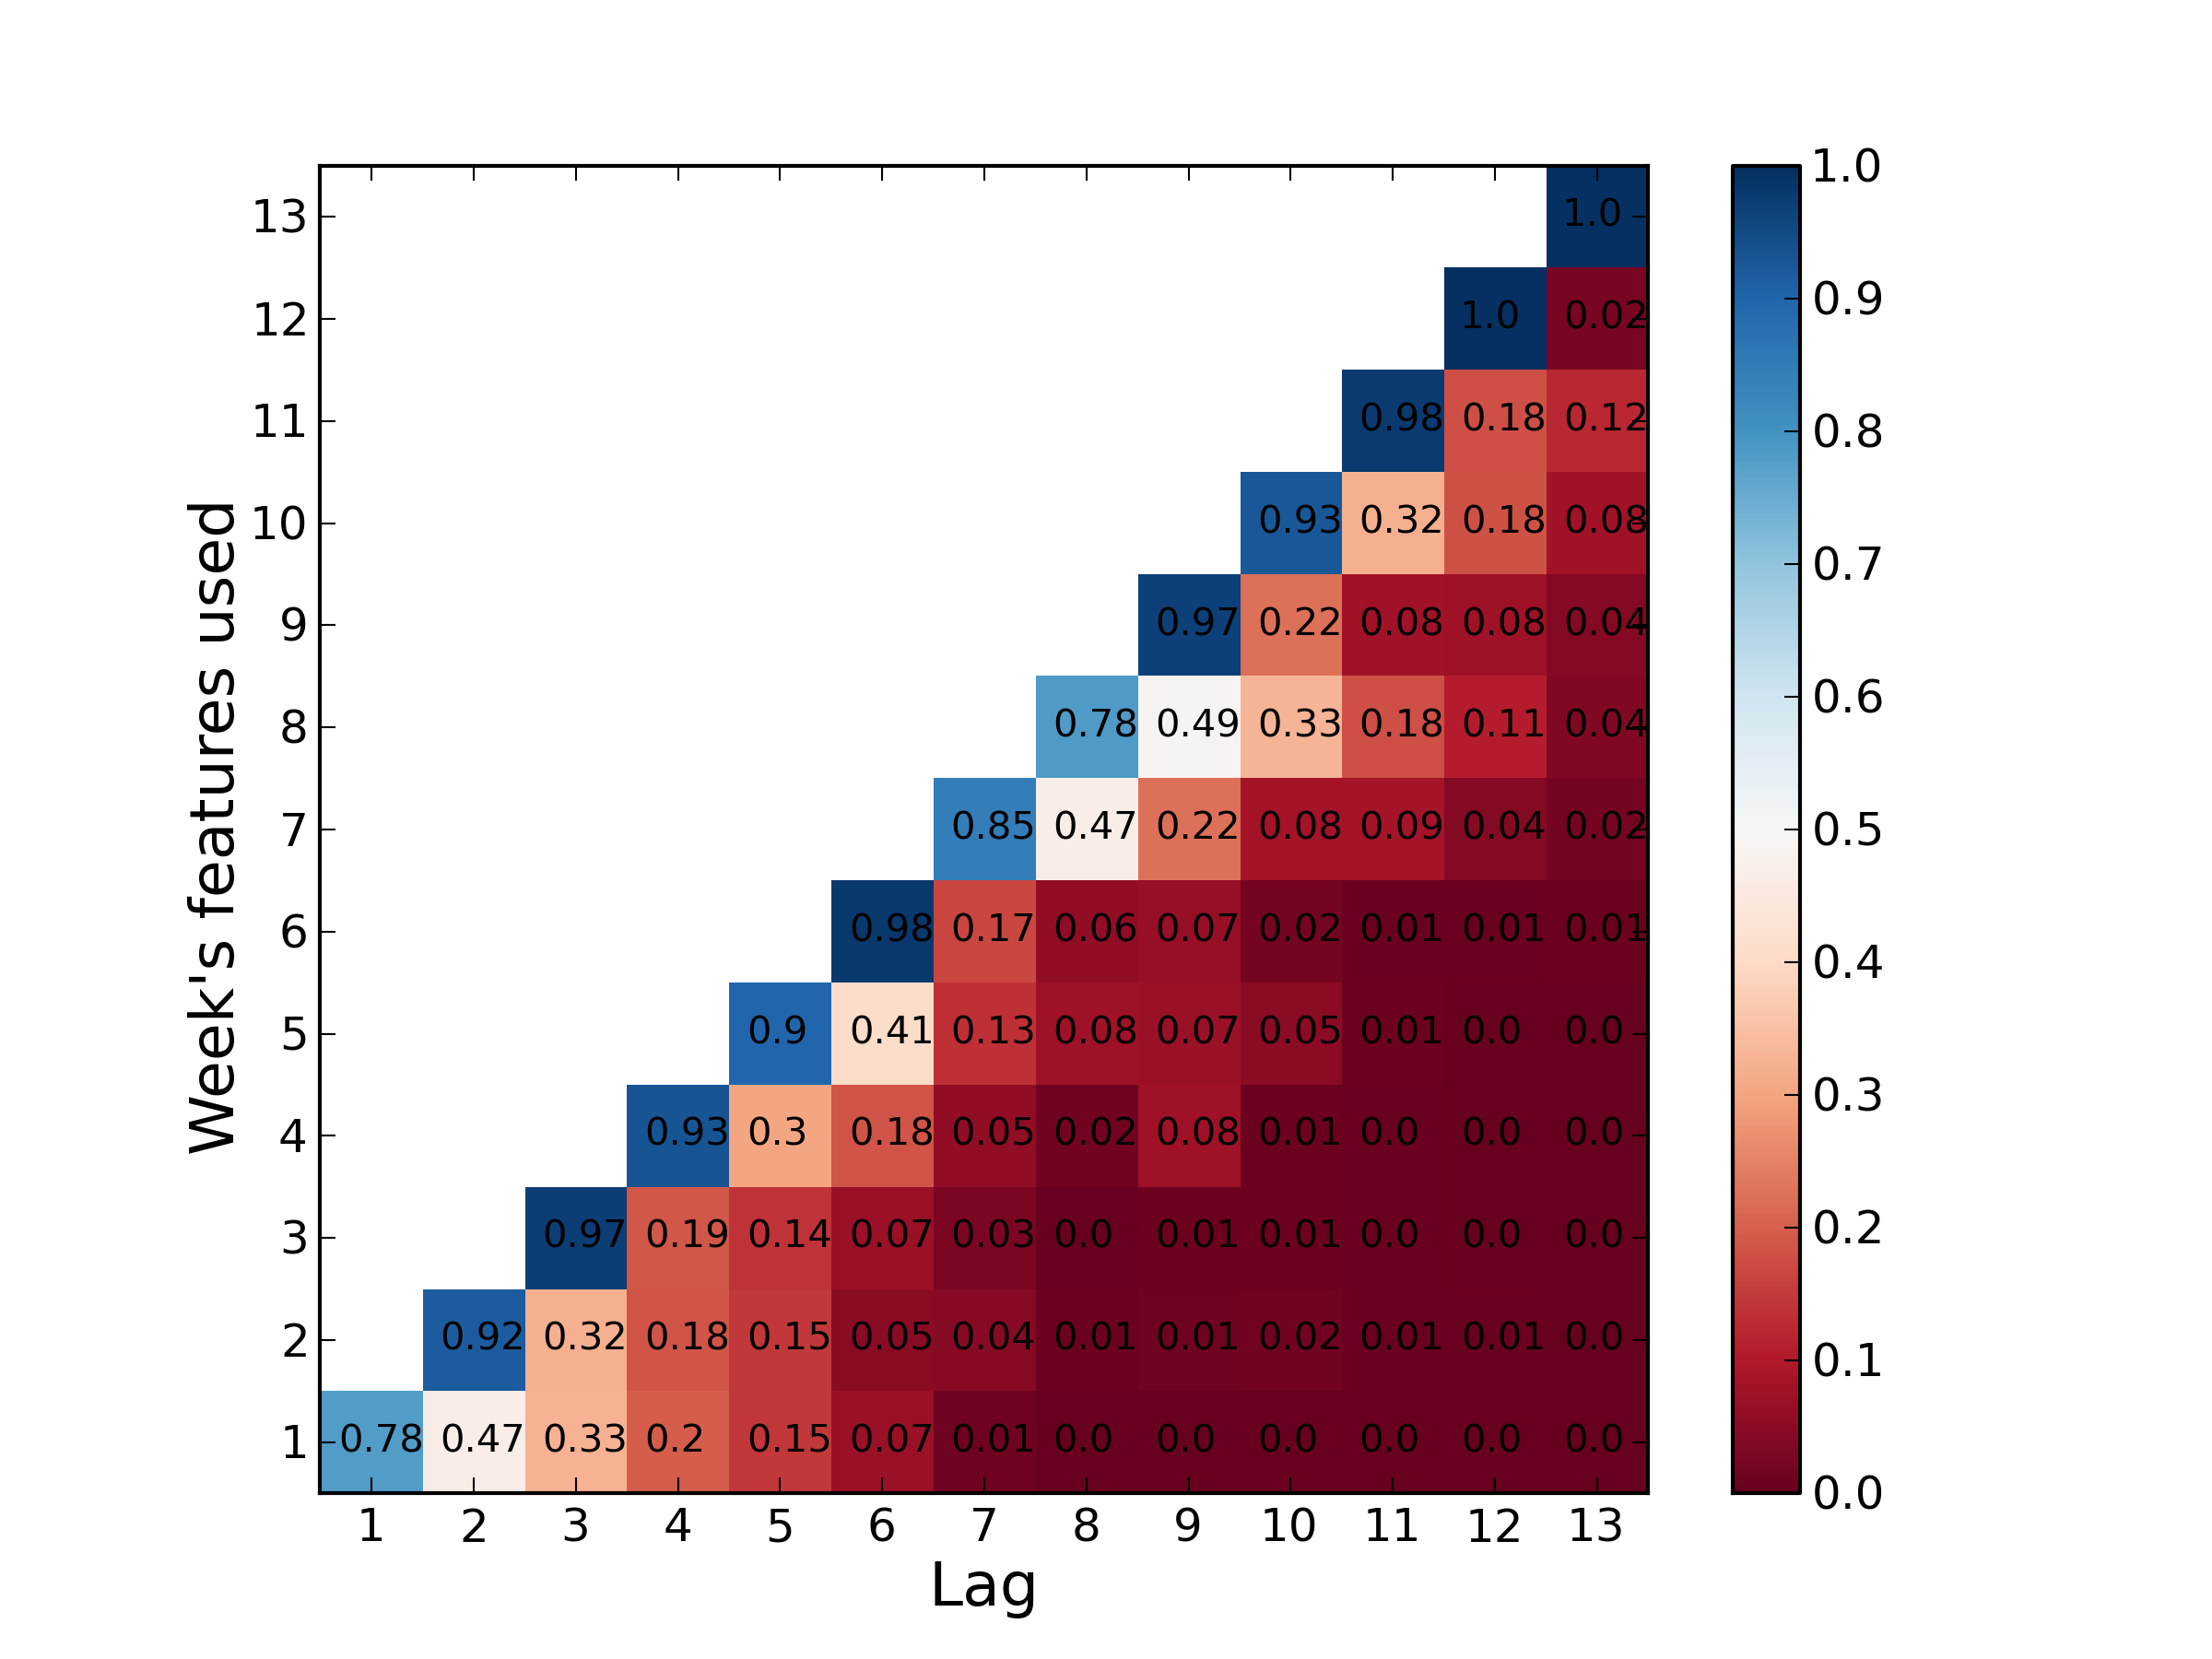
\includegraphics[width=0.9\textwidth]{figures/logreg/randomized_no_collab_over_time.png}
\end{figure}

\begin{figure}[ht!]
  \caption{Feature week's importance as \lag varies for the \forum cohort.}\label{fig:randomized_over_time_forum_only}
  \centering
    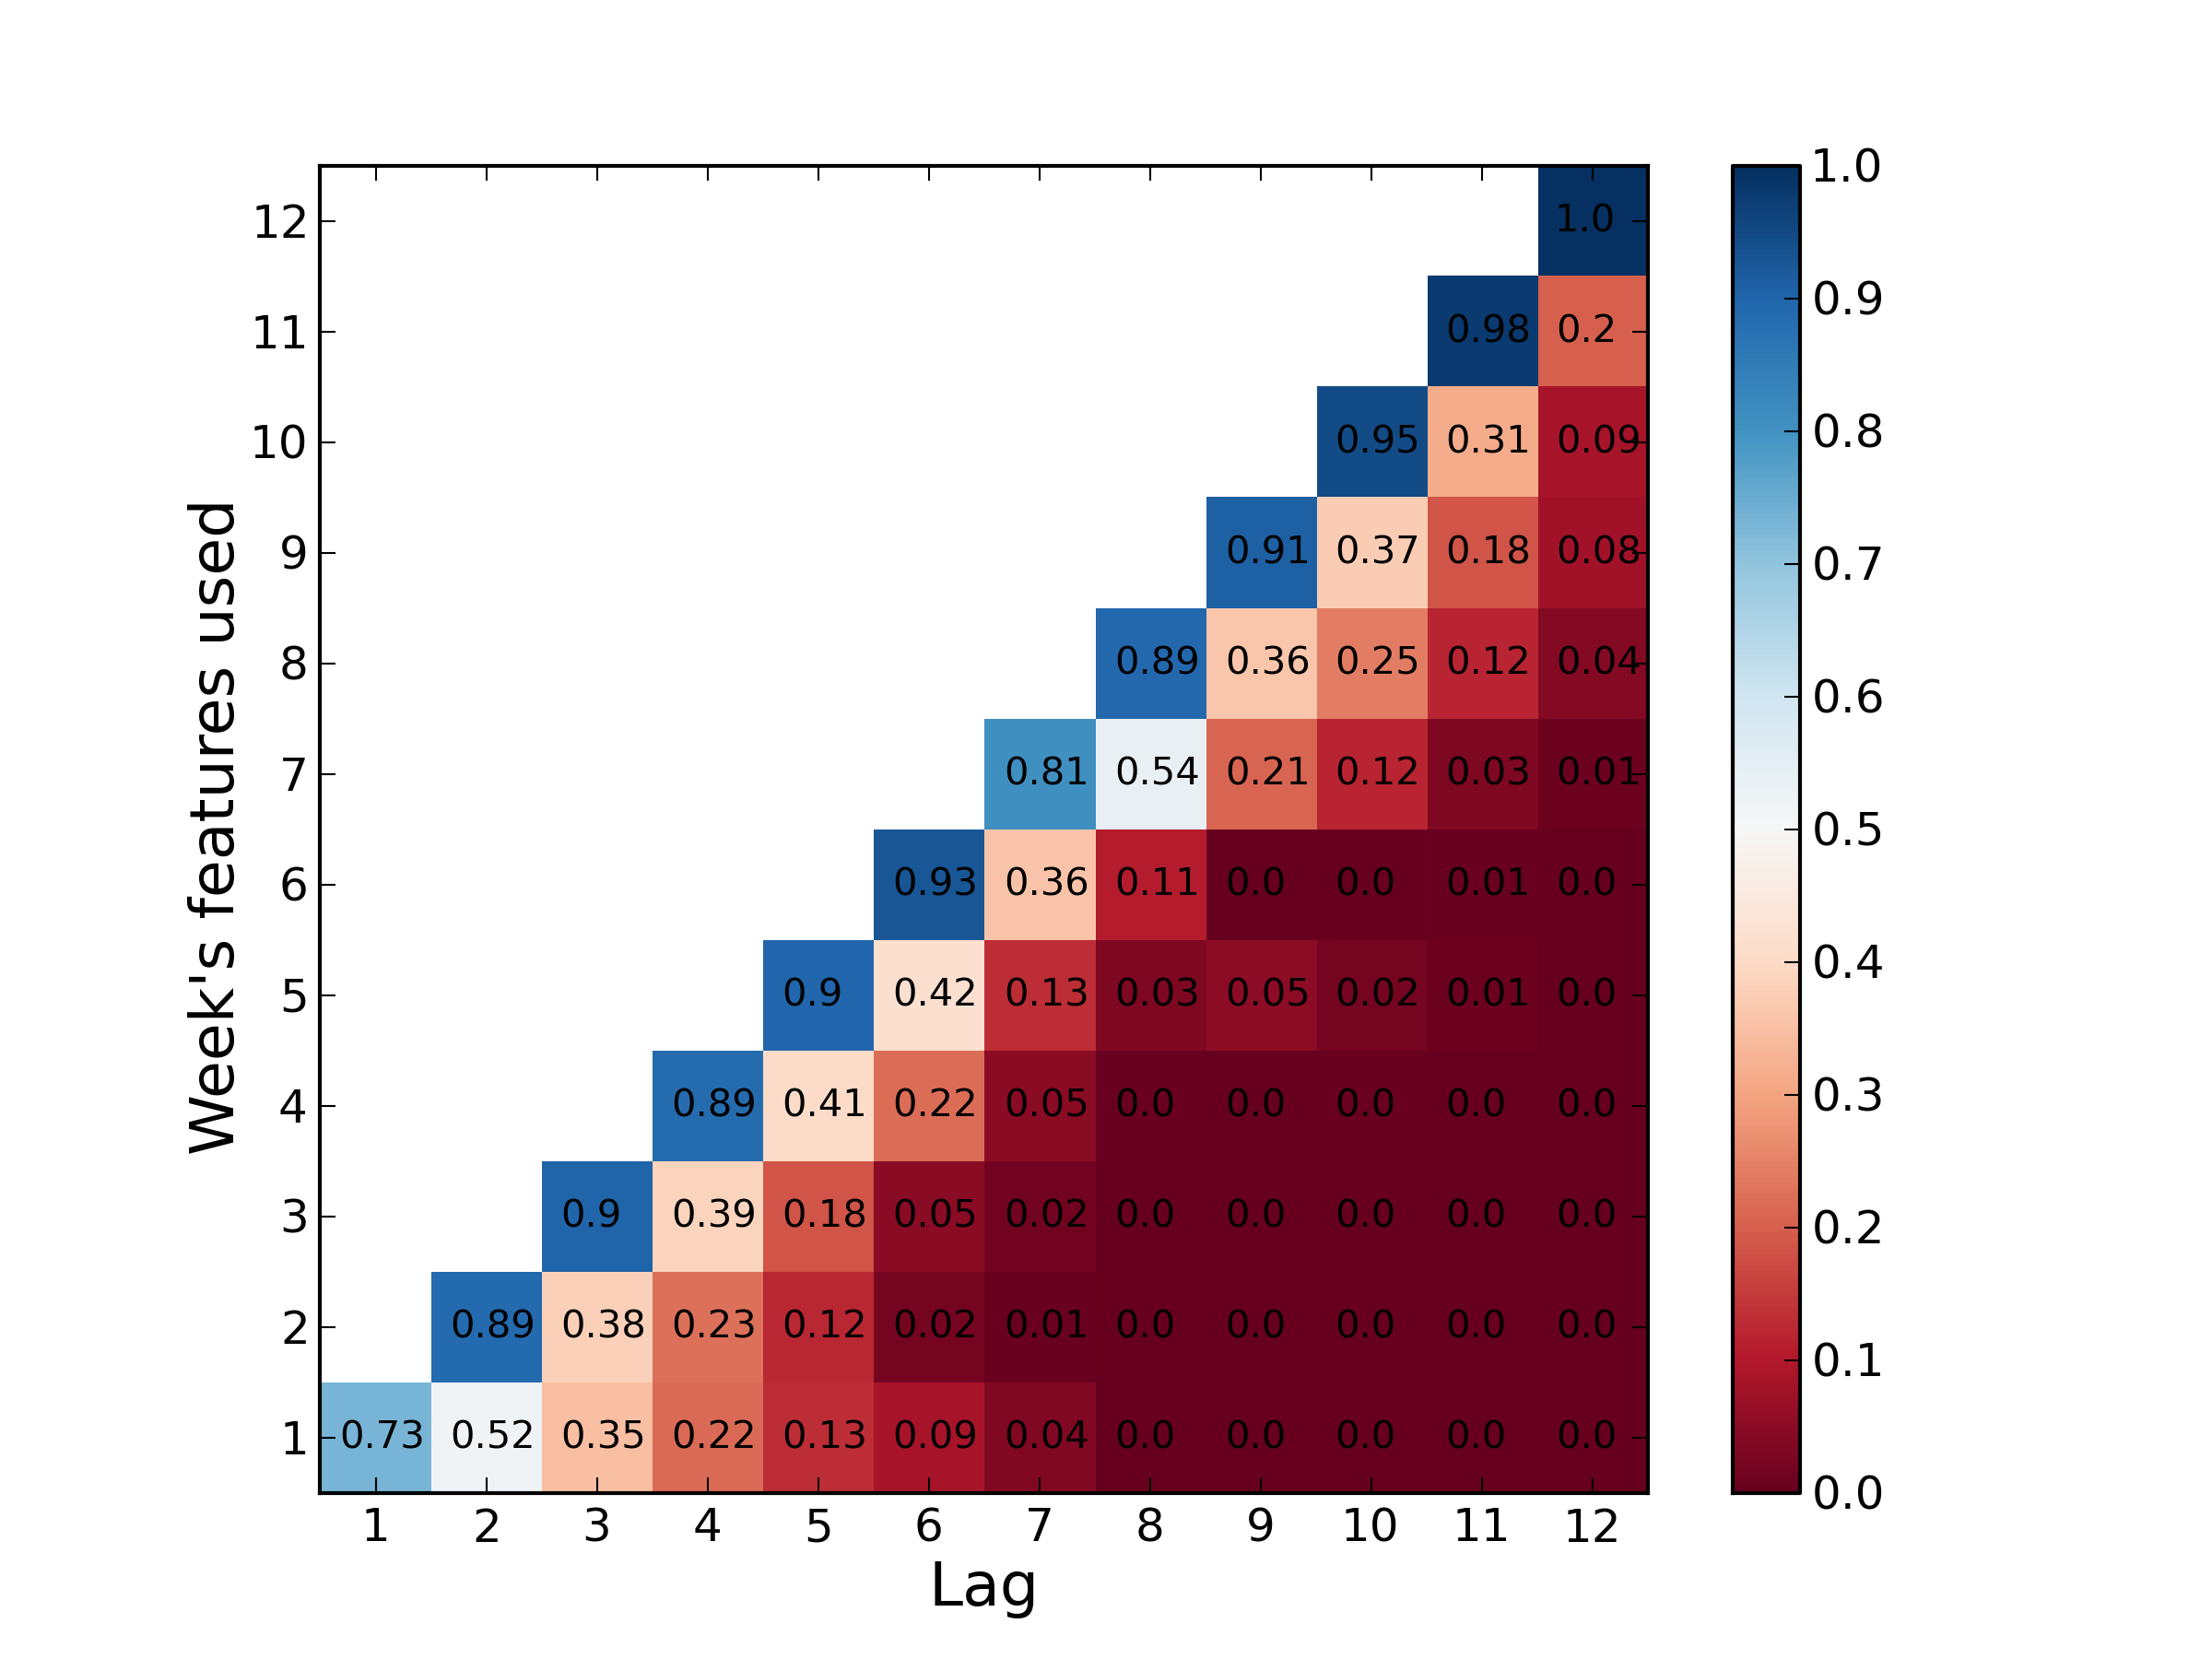
\includegraphics[width=0.9\textwidth]{figures/logreg/randomized_forum_only_over_time.png}
\end{figure}

\begin{figure}[ht!]
  \caption{Feature week's importance as \lag varies for the \both cohort.}\label{fig:randomized_over_time_forum_and_wiki}
  \centering
    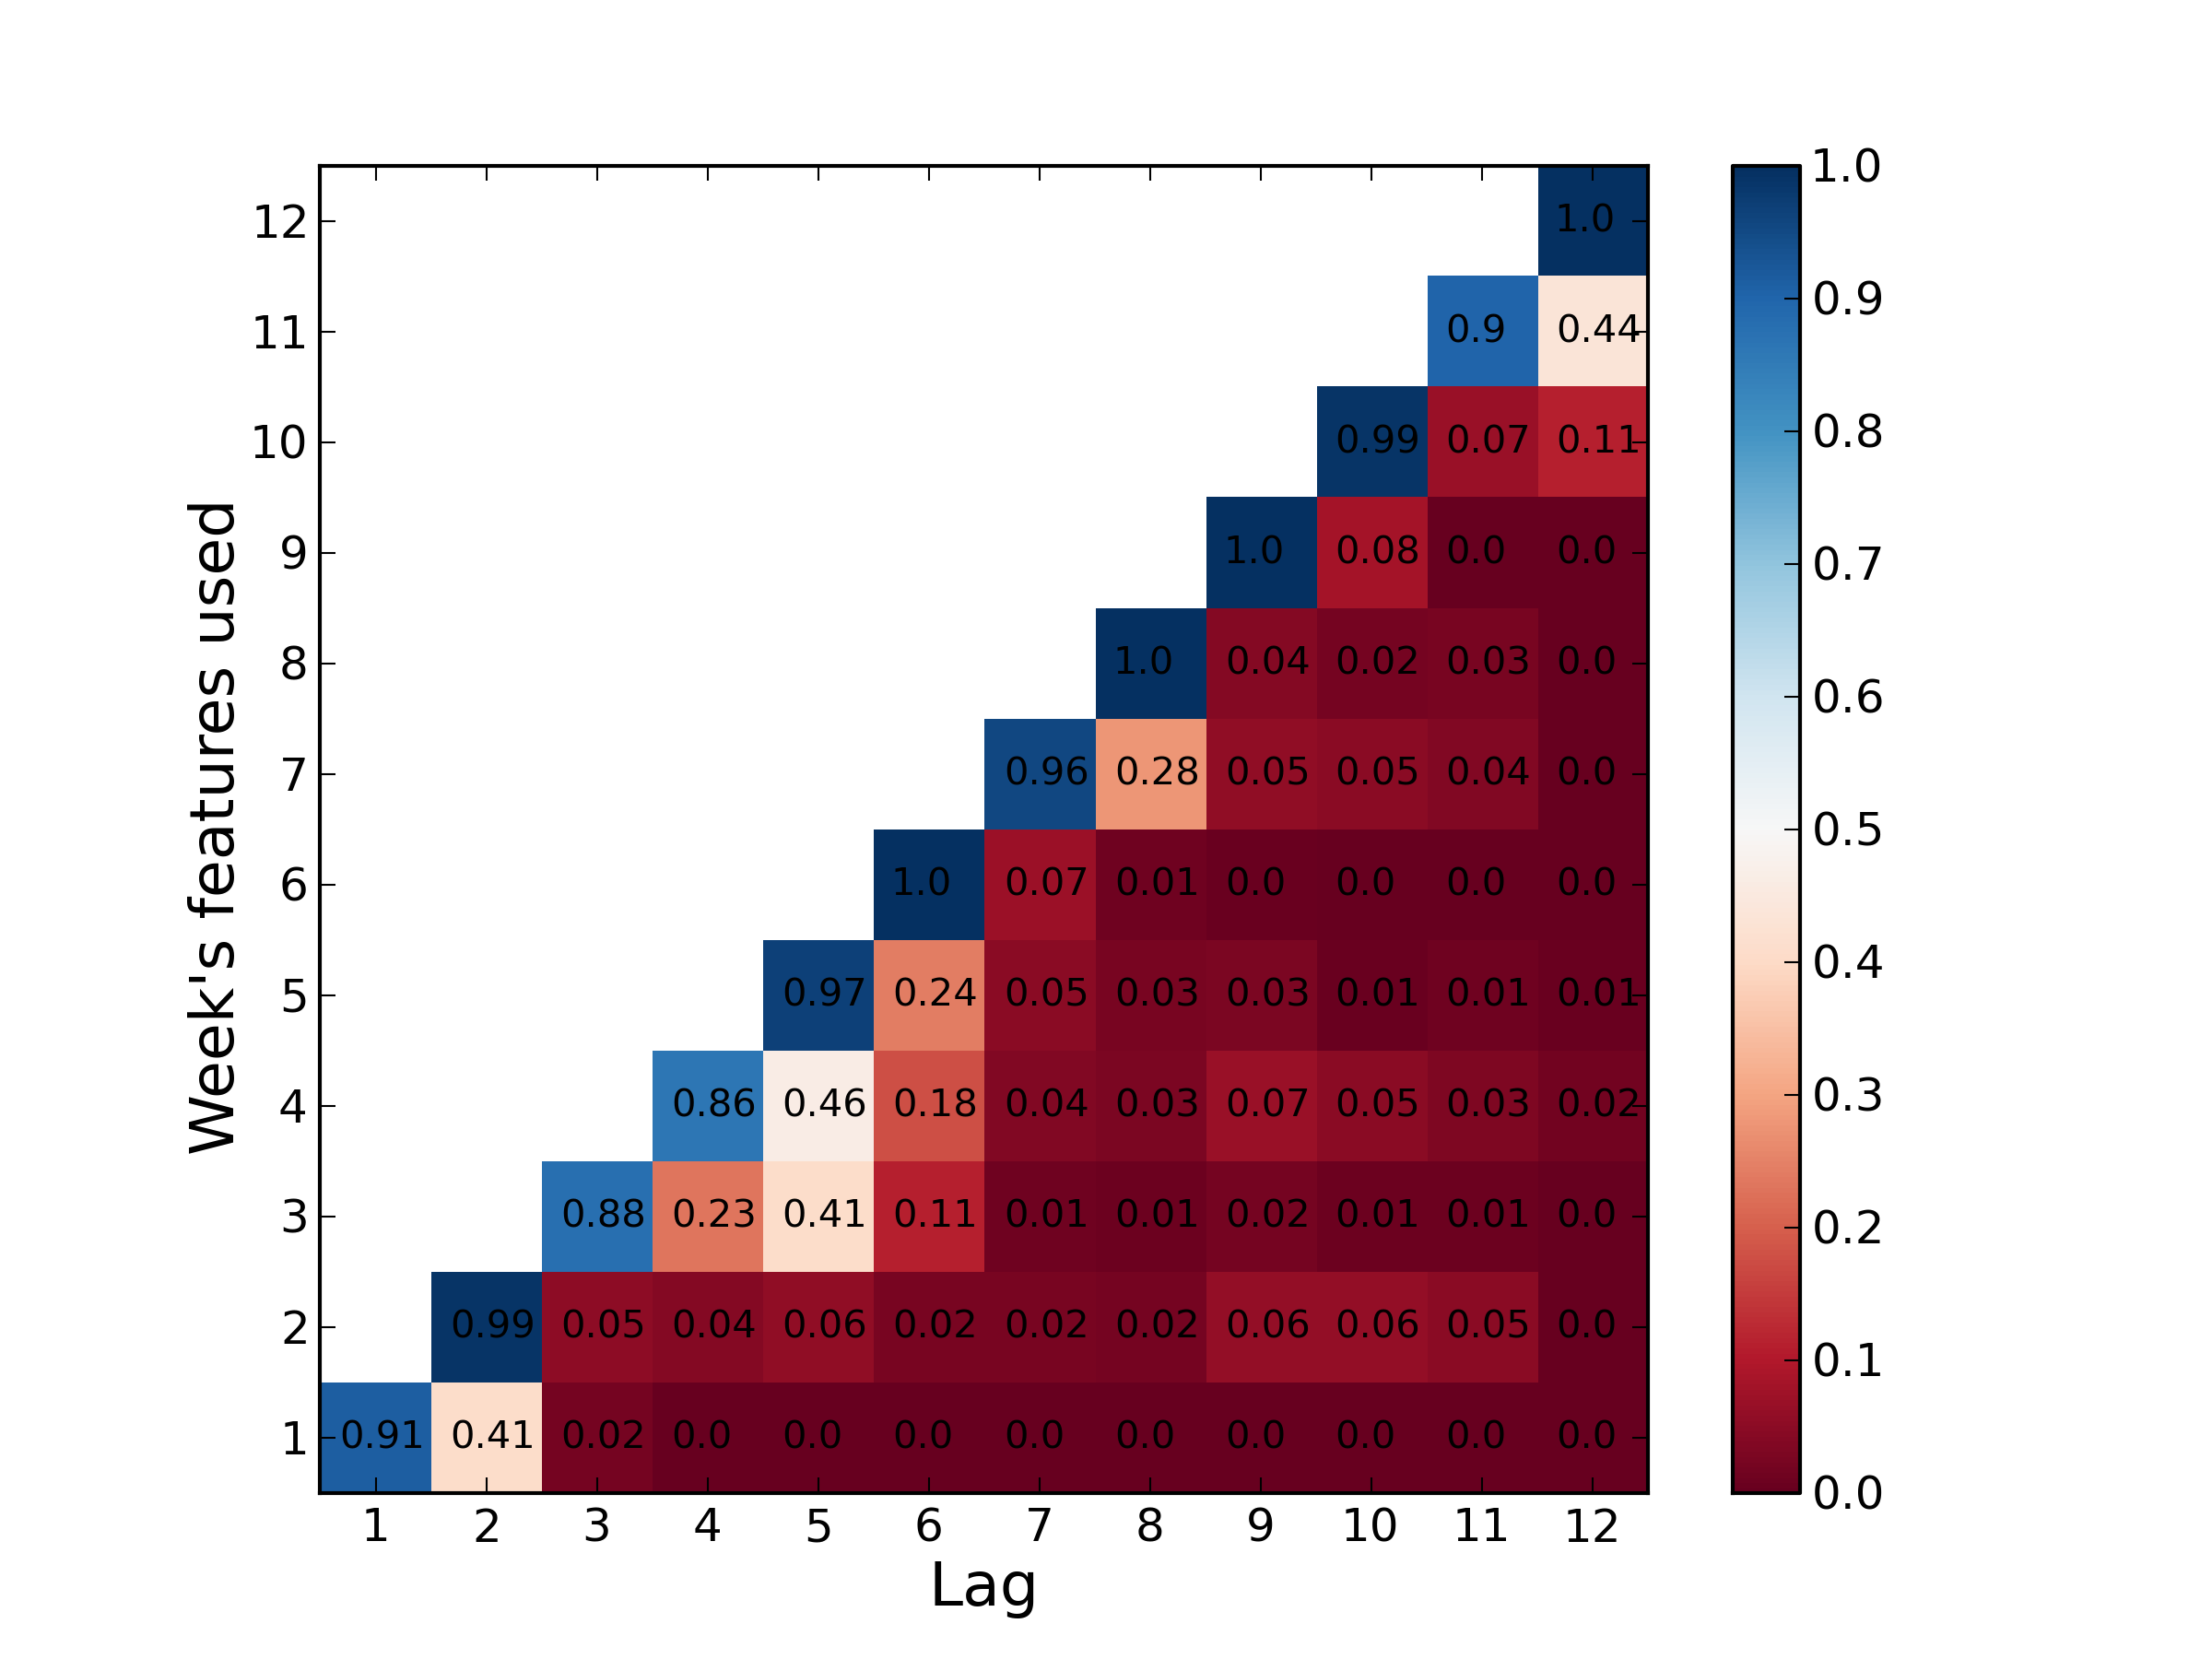
\includegraphics[width=0.9\textwidth]{figures/logreg/randomized_forum_and_wiki_over_time.png}
\end{figure}

\begin{figure}[ht!]
  \caption{Feature week's importance as \lag varies for the \wiki cohort.}\label{fig:randomized_over_time_wiki_only}
  \centering
    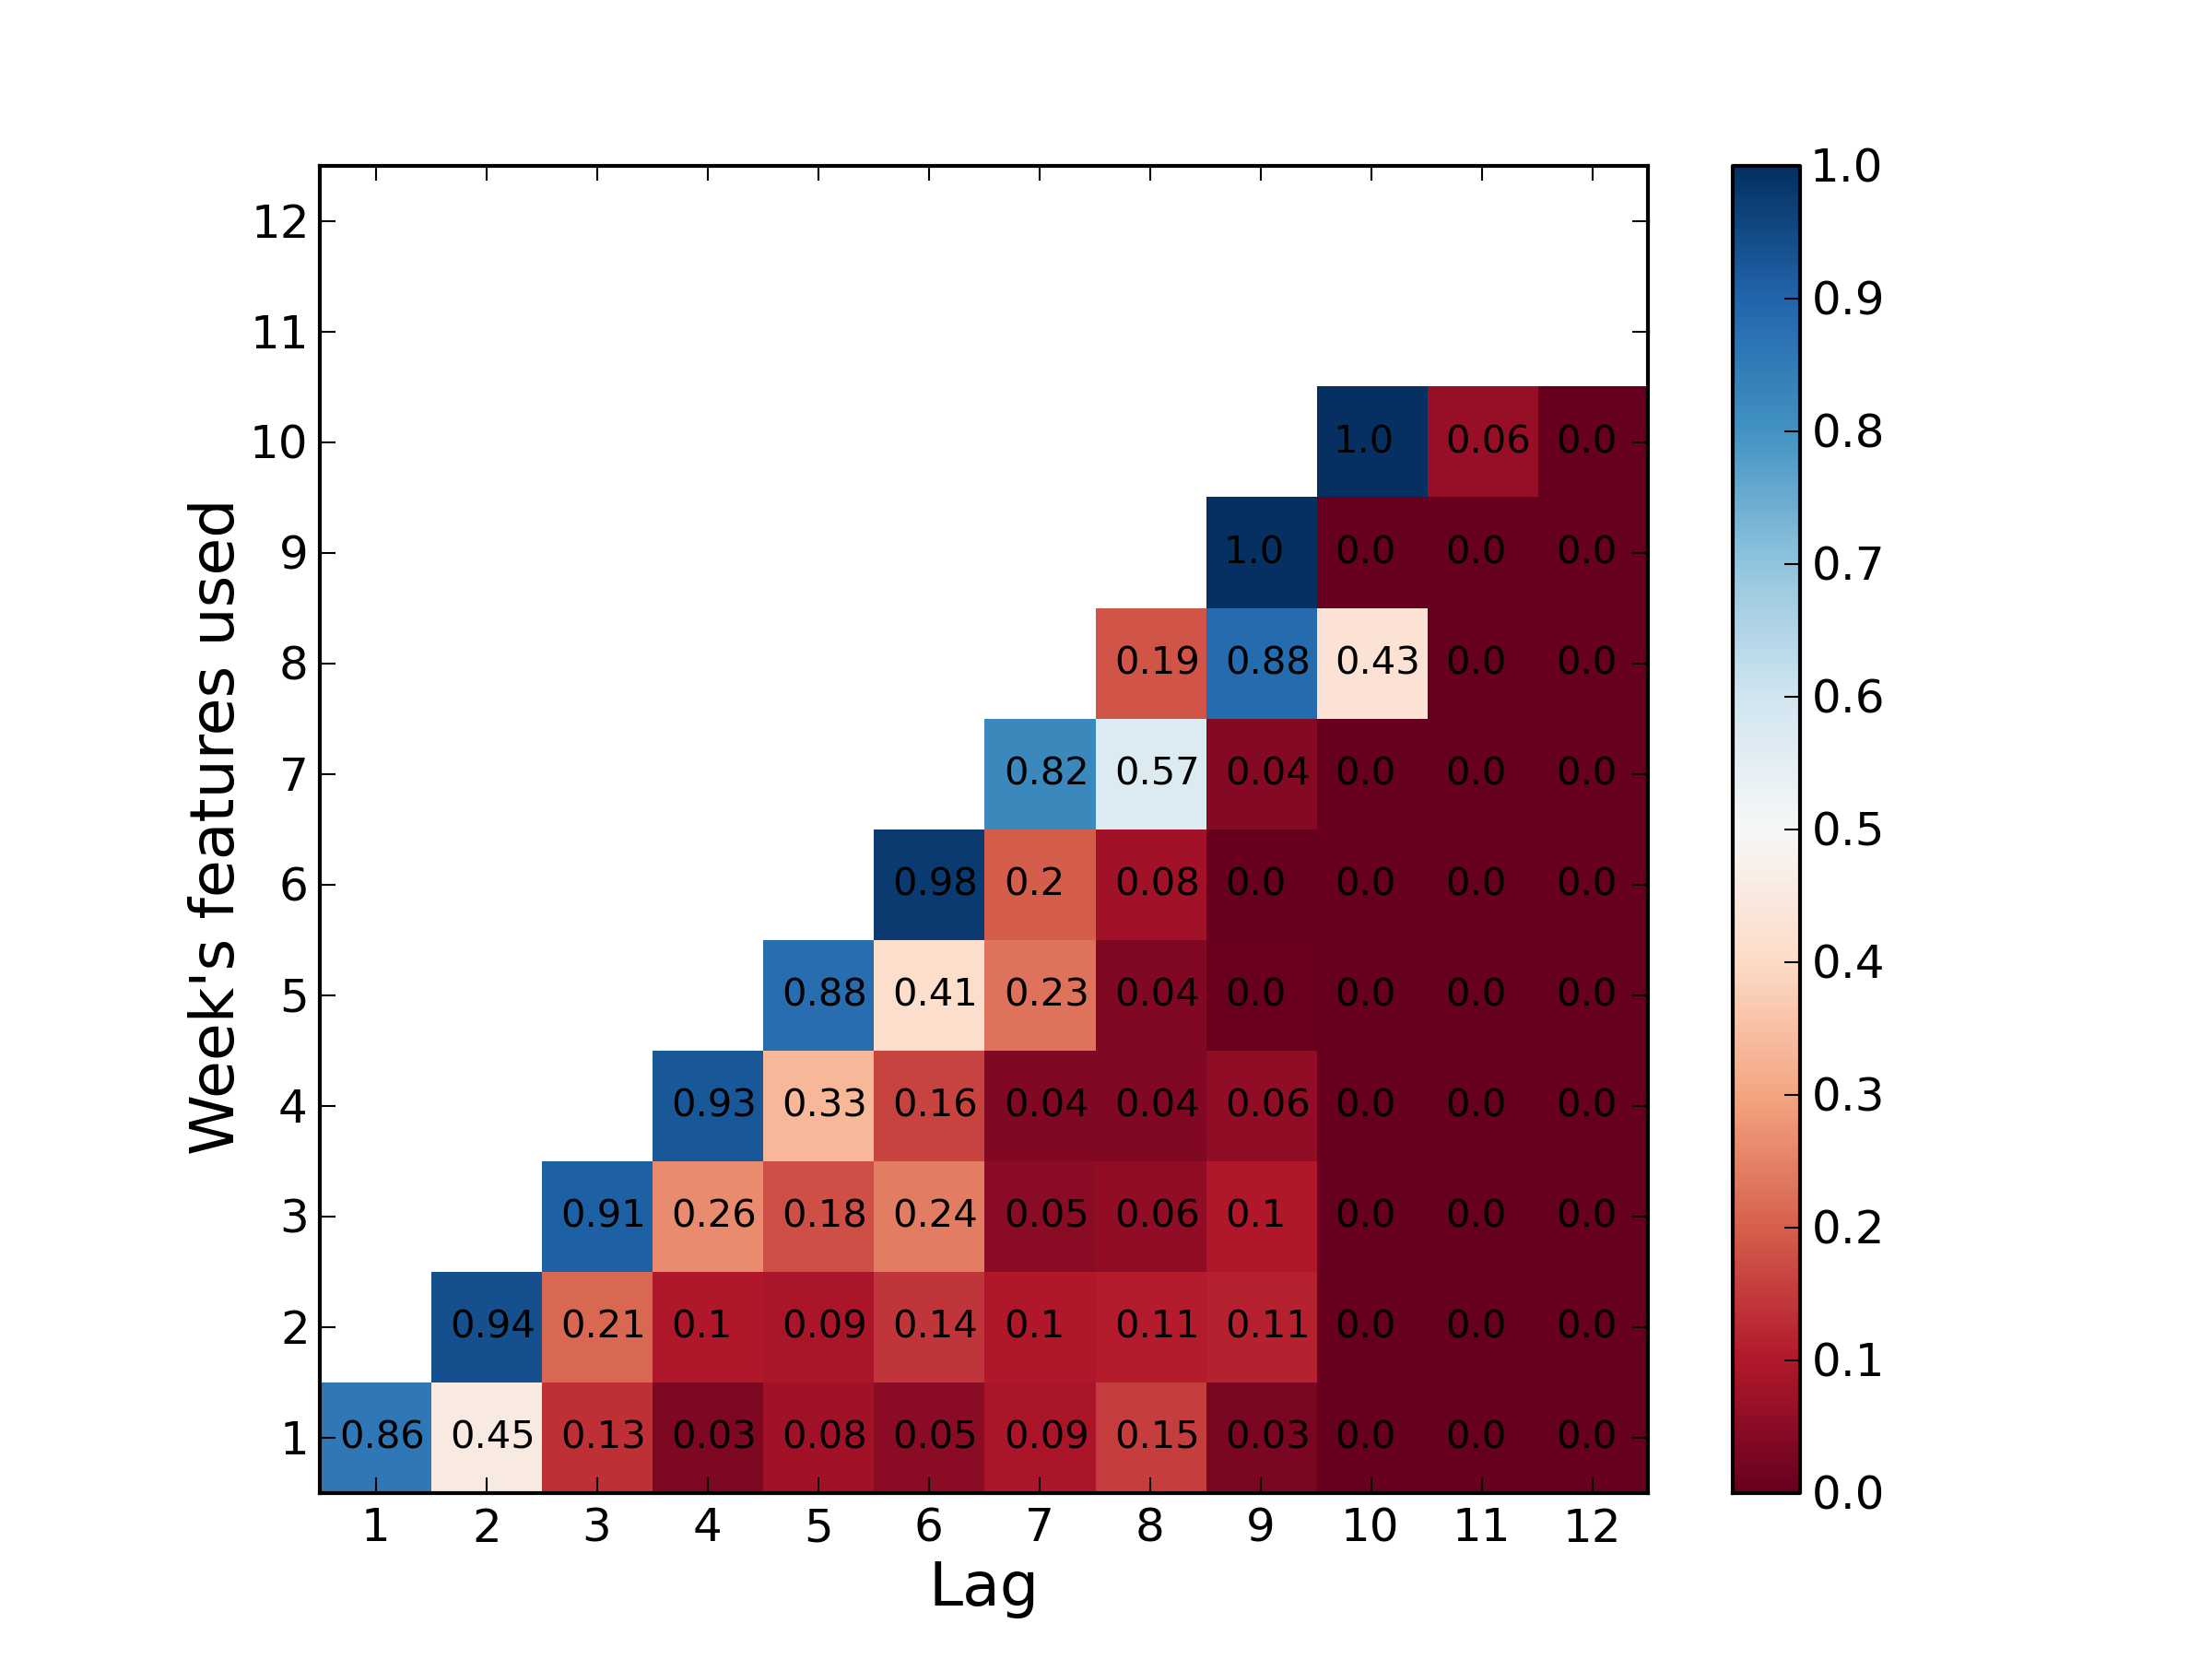
\includegraphics[width=0.9\textwidth]{figures/logreg/randomized_wiki_only_over_time.png}
\end{figure}

As expected, for each \lag, the week's features that mattered the most are the final weeks. This quickly drops off. For each cohort, the logistic regression models use approximately the last four weeks of data, regardless of the \lag. This indicates that there is not much added value in using more than four weeks of data as the \lag increases. This information would be useful when prediction must be done quickly, such as in real-time analytics.

\end{paragraph}





\chapter{Temporal Models of Student Behavior}\label{chap:hmm} 

In the previous chapter we presented a flat discriminative model to be able to predict \sti. In this chapter we present a methodology to model a student's data temporally. We posit that while taking a course a student has a latent state that represents a summary of his \textit{engagement} and \textit{interest} in the course during a particular week $i$. The \feat that we evaluated for the student for a week $i$ represent a draw from a multivariate distribution pertaining to that state. We posit that a student transitions from one state to another state during the course as the course transitions from one week to another. Using the data from multiple students our goal is to identify how many unique states there are, how students transition from state $i$ to state $j$ and what multivariate distribution of the \feat does each state represent? 

One way to achieve this is to cluster all students weekly data which is $15 \times N$ number of data points. Next, extract every student's cluster label on a weekly basis. We can then learn the transitions between the cluster labels across all students. An alternative approach presented in this chapter uses Hidden Markov Models (HMM) to jointly identify the multivariate distributions that each state represents and the transition probabilities between states.  

\section{Hidden markov models for modeling student behavior}
Hidden markov models, or HMMs, are a powerful and highly used class of \textit{generative} models. HMMs are usually built to model time series data, such as stock prices. They are a type of probabilistic graphical models in which the modeled entity is assumed to transition from one latent state to another as discrete time steps progress.  However, this state is not directly observable, and thus is `hidden.'  HMMs suppose that although the hidden state is not directly observable, the state relates to variables that are observable probabilistically. More specifically, each hidden state corresponds to a multivariate distribution for the observed variables from which they are most likely sampled from given the hidden state. The most basic HMM has only one observed variable (per time step), but the models we create contain 28 observed variables, one per feature\footnote{Most software libraries only support one observed variable. This is because using multiple observed variables is computationally complex}. Figure \ref{fig:hmm} shows the graph structure of a typical HMM. In the figure, Z (shaded node) represents a hidden node. The graphical form as shown in the Figure~\ref{fig:hmm} can be written as a joint distribution given by: 

\begin{equation}
p(z_{1:T},\bar{x}_{1:T})=p(z_1)\prod_{t=2}^T p(z_t|z_{t-1}) \prod_{t=2}^T p(\bar{x}_t|z_t)
\end{equation}
In the most common case, independence is assumed among the observed variables given the hidden variable, making the joint distribution:
\begin{equation}
p(z_{1:T},\bar{x}_{1:T})=p(z_1)\prod_{t=2}^T p(z_t|z_{t-1}) \prod_{t=2}^T \{ \prod_{i=1}^m p({x^i}_t|z_t)\}
\end{equation}

The observed variables can be either continuous, or discrete. In the continuous case, the distribution for observed variables is typically assumed to be independent univariate Gaussian. In the discrete case, a multinomial distribution is used to represent the joint distribution between the hidden variable and the observed variable.  Note that, when using multinomial distribution, observed values are no longer ordinal, but are nominal, i.e., A is not greater or less than B, rather is simply not B. To use this model when the variables are continuous the variables are binned using a methodology that preserves the entropy of the univariate distribution for that variable (presented in section \ref{section:binning}).

Let us assume that the hidden variable takes one of the $k$ values $1 \dots K$ and each observed variable has $1 \dots P$ discrete values. The model is parametrically defined by a $K$-by-$K$ transition matrix and $m$,  $K$-by-$P$ emission matrices, one for each of the observed variable given the hidden variable and a 1-by-K probability vector for the initial state $p(z_1)$. 

The entry $i,j$ in the transition matrix shown below represents the probability $p(z_t=i |z_{t-1}=j)$ and is given by: 
\begin{equation}
A_{i,j} =
 \begin{pmatrix}
  a_{1,1} & a_{1,2} & \cdots & a_{1,k} \\
  a_{2,1} & a_{2,2} & \cdots & a_{2,k} \\
  \vdots  & \vdots  & \ddots & \vdots  \\
  a_{k,1} & a_{k,2} & \cdots & a_{k,k}
 \end{pmatrix}
\end{equation}

and the emission matrix for $p^{th}$ observed variable is given by:

\begin{equation}
E_{i,j} =
 \begin{pmatrix}
  e_{1,1} & e_{1,2} & \cdots & e_{1,p} \\
  e_{2,1} & e_{2,2} & \cdots & e_{2,k} \\
  \vdots  & \vdots  & \ddots & \vdots  \\
  e_{k,1} & e_{k,2} & \cdots & e_{k,p}
 \end{pmatrix}
\end{equation}


The entry $i,j$ in the emission matrix for variable $m$ represents $p(x_t^m=i | z_t=j)$. The objective of training an HMM is to find the optimal \textit{transition} and \textit{emission} probabilities given the graphical structure. 
\begin{figure}[ht!]
  \caption{A typical hidden markov model structure. Top figure shows a common hidden markov model with only one variable. The bottom figure represents our case where we have multiple observed variables per time slice.}\label{fig:hmm}
  \centering
    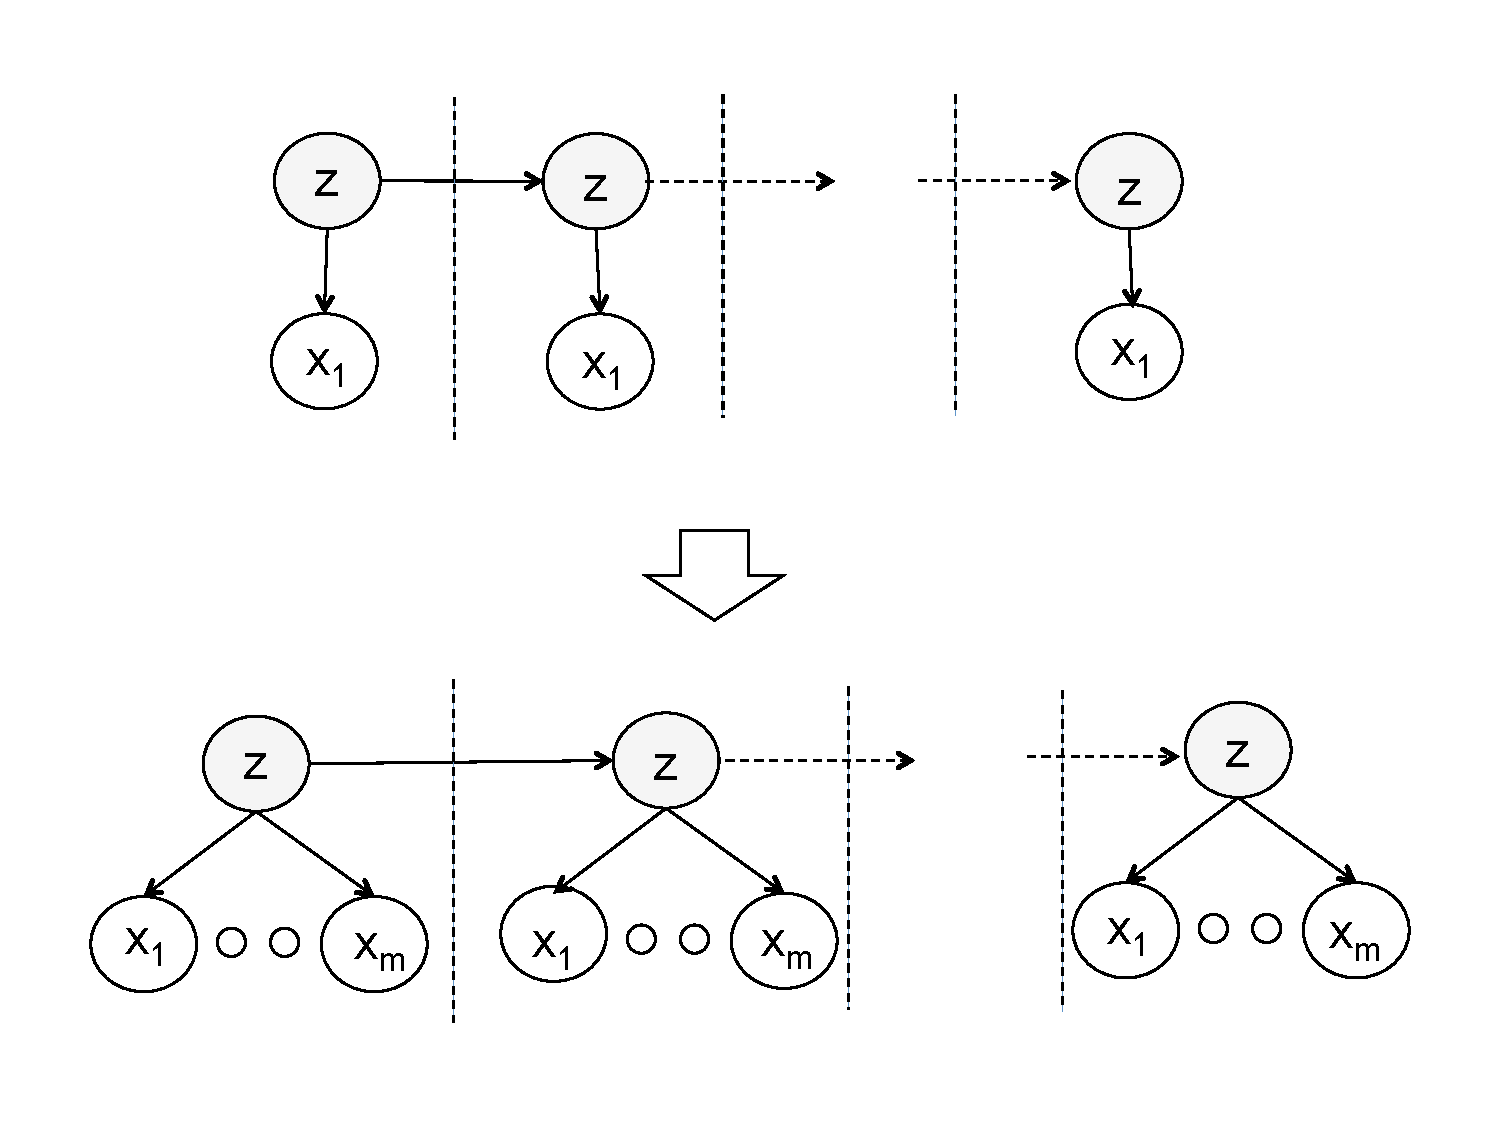
\includegraphics[width=1.0\textwidth]{figures/one-vs-multi}
\end{figure}

\subsection{Learning the probabilities of an HMM}
A hidden markov model is typically constructed using the Baum-Welch algorithm. Firstly, the initial states, transition matrices and emissions matrices are assigned (usually randomly). In each iteration of Baum-Welch, a forward-backwards inference algorithm is used to estimate the $p(z_t|\bar{x})$ for all $t$ and for all sequences given the parameters. Subsequent to this estimation, the 
 the emissions and transition matrices are updated.  As the parameters are updated, a log-likelihood score is evaluated to measure how well the model fits the data. In each iteration, the likelihood improves, and will begin to converge on either a local or global maximum.The algorithm terminates after the difference between log-likelihood of two consecutive iterations falls below a threshold (implying convergence), or a maximum number of iterations is reached. Through training, the model learns both the distributions of observed variables for each state, and the probabilities of transitioning from one state to another.

Figures \ref{fig:hmm_training} demonstrates how the observed variables are used as evidence in order to train the HMM.


\begin{figure}[ht!]
  \caption{This figure shows how the student-week-matrix which has features that represent the behavior of a student during a week is provided as evidence to the hidden markov model training.}\label{fig:hmm_training}
  \centering
    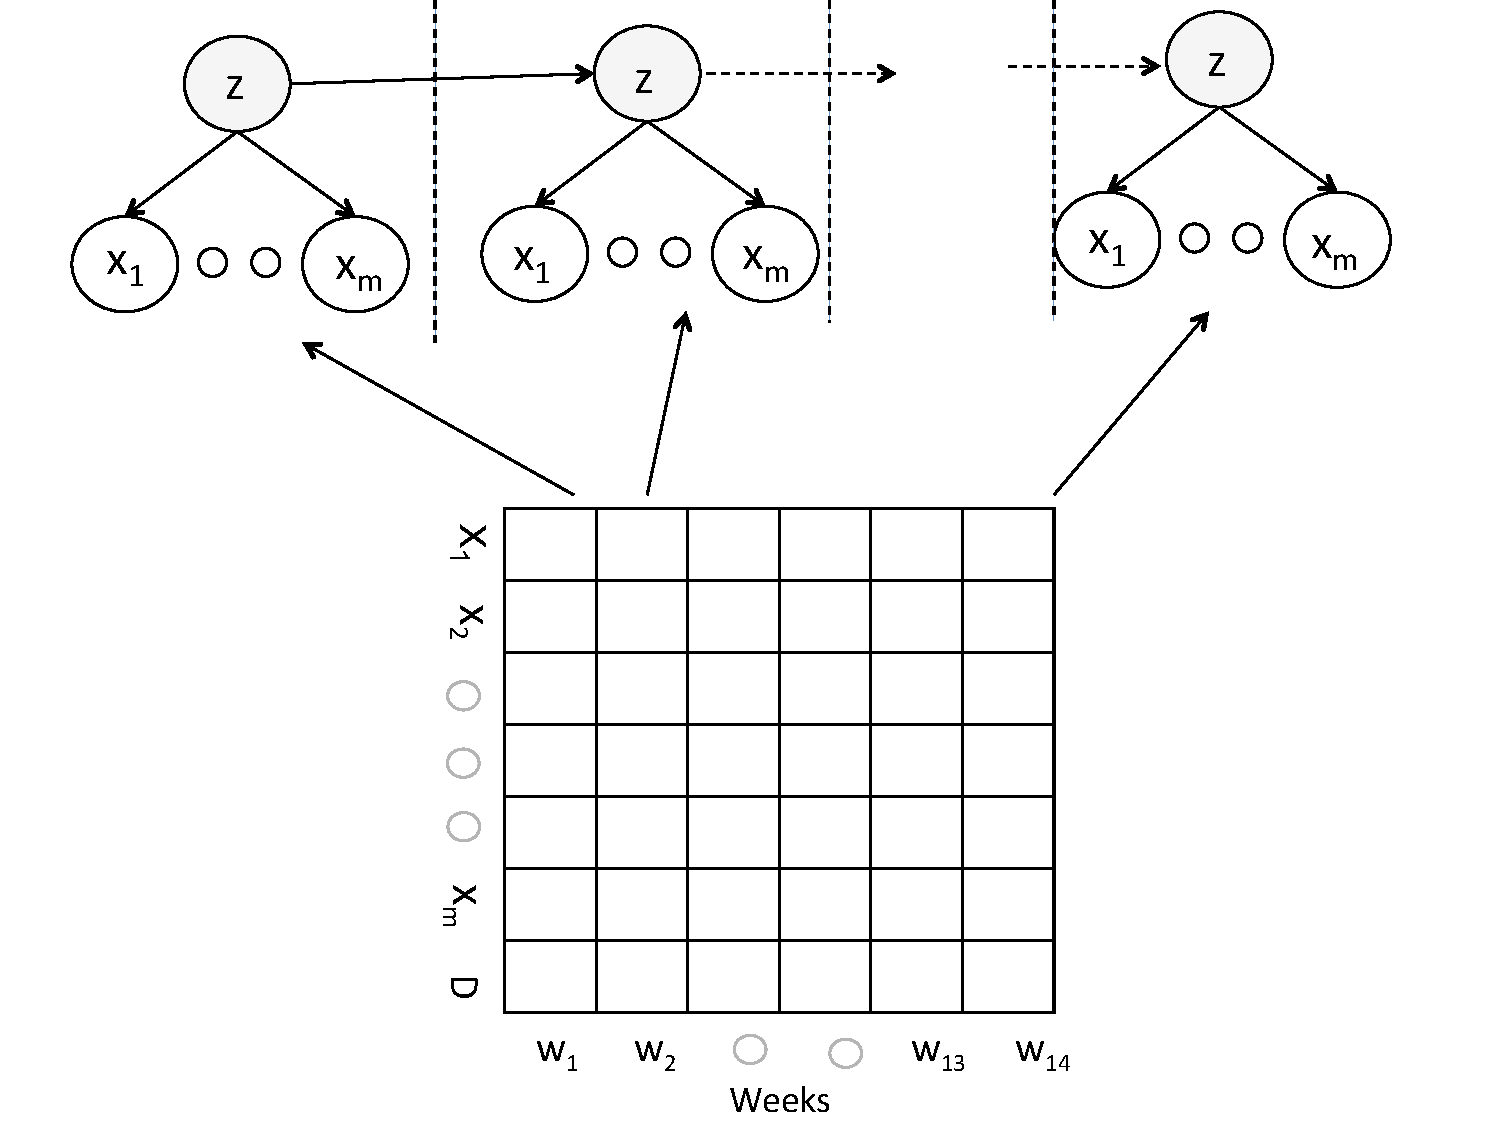
\includegraphics[width=0.7\textwidth]{figures/week_matrix_to_hmm}
\end{figure}

\subsection{Inference}
Once the HMM is built, we can utilize it to predict a future value of an observed variable. In our case, we can predict the \sti variable for a future week. Figure \ref{fig:hmm_predict} shows this use of an HMM as a prediction engine. An alternative inference goal is to find the probabilities for each hidden state at a given future timestep. Inference is performed using the forward-backwards algorithm.

\begin{figure}[ht!]
  \caption{This figure shows how the HMM is used to predict value for an observed variable in a future time slice. In this specific example evidence is provided to the model through week 2 and a prediction is sought for the 14th week }\label{fig:hmm_predict}
  \centering
    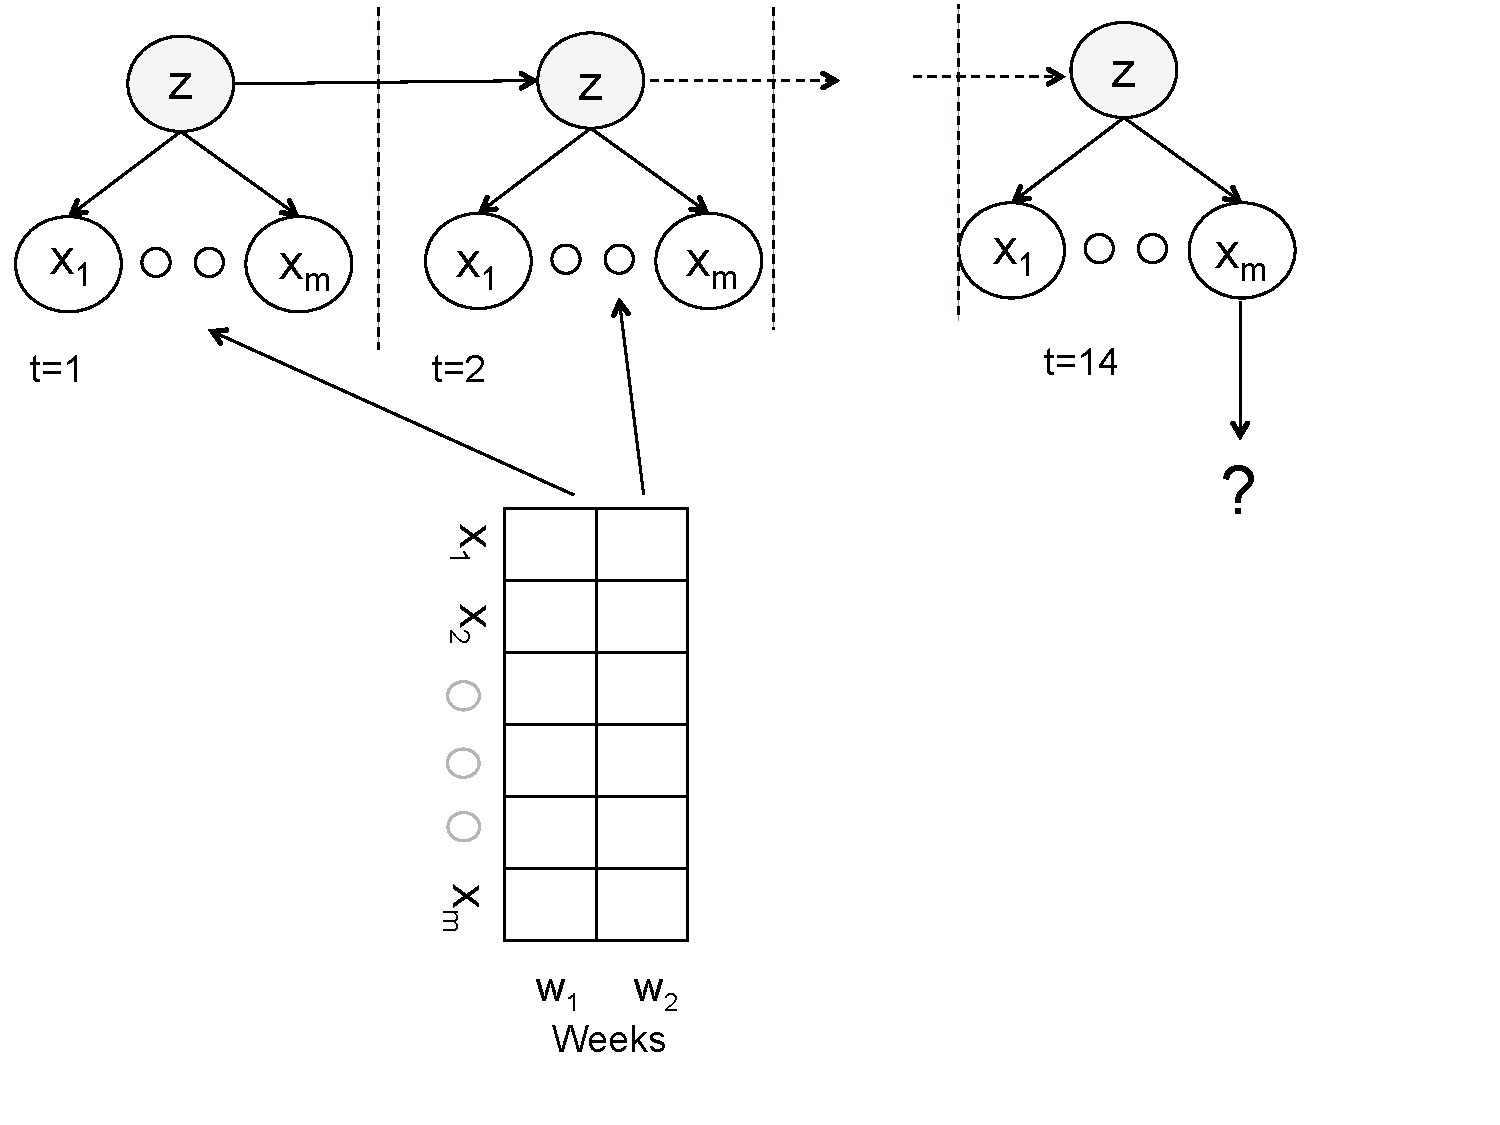
\includegraphics[width=0.7\textwidth]{figures/hmm-as-predict}
\end{figure}

\subsection{Advantages and disadvantages of HMMs} 
\begin{itemize}
\item Hidden markov models are designed for time sequenced data. They allow for repeating features across time sequences. 
\item HMMs hidden state provide some intuitive notion of clustering types of students by way of the hidden state. For example, if a model with a hidden support of 4 delivers fantastic predictive power, we could surmise that there are really 4 modes an entity can be in. Indeed, the emission probabilities of the hidden states might provide insights about what the modes may represent. In the stopout prediction problem, for example, the modes might represent different levels of engagement in the course, and represent the true state of a student in a given timestep. However, apart from such a scenario, HMMs often become a black box predictive model. For example, there is no notion of feature weights. 
\item HMMs require a lot of computing power to train, and the training time grows exponentially with the number of time sequences (this is offset through dynamic programming techniques, but is still slow). 
\item Hidden markov models assume independence between the observed variables given a hidden variable, which is often not the case (such as in our feature-set which uses derived features). Training a more complicated graph is possible, but much more computationally intensive.
\item The Baum-Welch algorithm can get stuck on local maxima of probabilities as it converges.
\end{itemize}

\section{Predicting stopout using HMMs}
We trained hidden markov models with the objective of predicting student persistence. We used the 28 (27 interpretive features + binary stopout feature) as described in chapter 3 as the observed variables of the hidden state. We applied inference to the trained models, asking the HMM to generate the probabilities of sampling the \sti value for a future timestep.

Each experiment used a given lead as a parameter. For example, for a lead of 1, we used features from week 1 to predict week 2, then features from 1 and 2 to predict week 3, etc. Note that this prediction problem is subtly different from that of the logistic regression. In logistic regression, we chose a lead and a lag, and predicted a single week's stopout value. Here, we choose a lead, and use every possible lag with that lead in order to predict every week up until the end of the course. However, as in logistic regression, we do not perform inference on weeks where the student is already known to have stopped out.

Hidden markov models require several parameter choices. Because the correct hidden support value is unknown in hidden markov models, we varied this parameter to find an optimal value. We used a range of supports from 3 to 29, with a step size of 2. We stopped at 29 for the sake of computing time. We used 100 iterations as the maximum number of Baum-Welch iterations along with a log-likelihood differential threshold of 0.0000001. Training stopped when one or the other was reached.

\subsection{Experimental setup}
To build a predictive HMM, we did the following on every lead, hidden support and cohort combination
\footnote{We first used a Matlab implementation of Dynamic Bayesian Networks in order to build HMMs. This toolbox was flexible enough to construct arbitrary graphical structures, including HMMs. However, this toolkit proved too slow to use, even at scale. We switched to a custom built implementation of hidden markov models. The code was written in C++ by two members in the ALFA group. It was orders of magnitude faster, but provided a much cruder interface to use. After a lot of testing, and benchmarking, we achieved as good of results as with the MATLAB implementation given a large dataset, and with much faster time. Consequently, we recommend any sizable machine learning/data science project to use C++}:

\begin{enumerate}
\item Performed 10 fold cross validation on the training set. In order to speed this process up, we ran each in parallel using python's Parallelization package.
\item Trained an HMM on the entire train dataset. To compensate for the fact that HMMs often get stuck on local maxima as they train, we trained 10 models for each experiment. We selected the best model to use based on the likelihood score of the Baum-Welch algorithm. We also performed this in parallel, as training can take significant amounts of time.
\item Performed inference on the test dataset by putting each data point through best model. Specifically, we asked the model for the probabilities of each stopout value for a given week. We compared the resulting probability of stopout versus the truth stopout label.
\item Evaluating the model using mean cross-validation ROC AUC and test set ROC AUC.
\end{enumerate}

\section{HMM results}
Our hidden markov models performed well at predicting stopout.  Overall, we saw a fairly sharp decline in accuracy as the lead increased, especially as compared with logistic regression. Similar to logistic regression, different cohorts achieved very different prediction accuracies as well.

\begin{figure}[ht!]
  \caption{Heatmap for the \neither cohort. PCA transformations of features used.}\label{fig:hmm_heatmap_no_collab_pca}
  \centering
    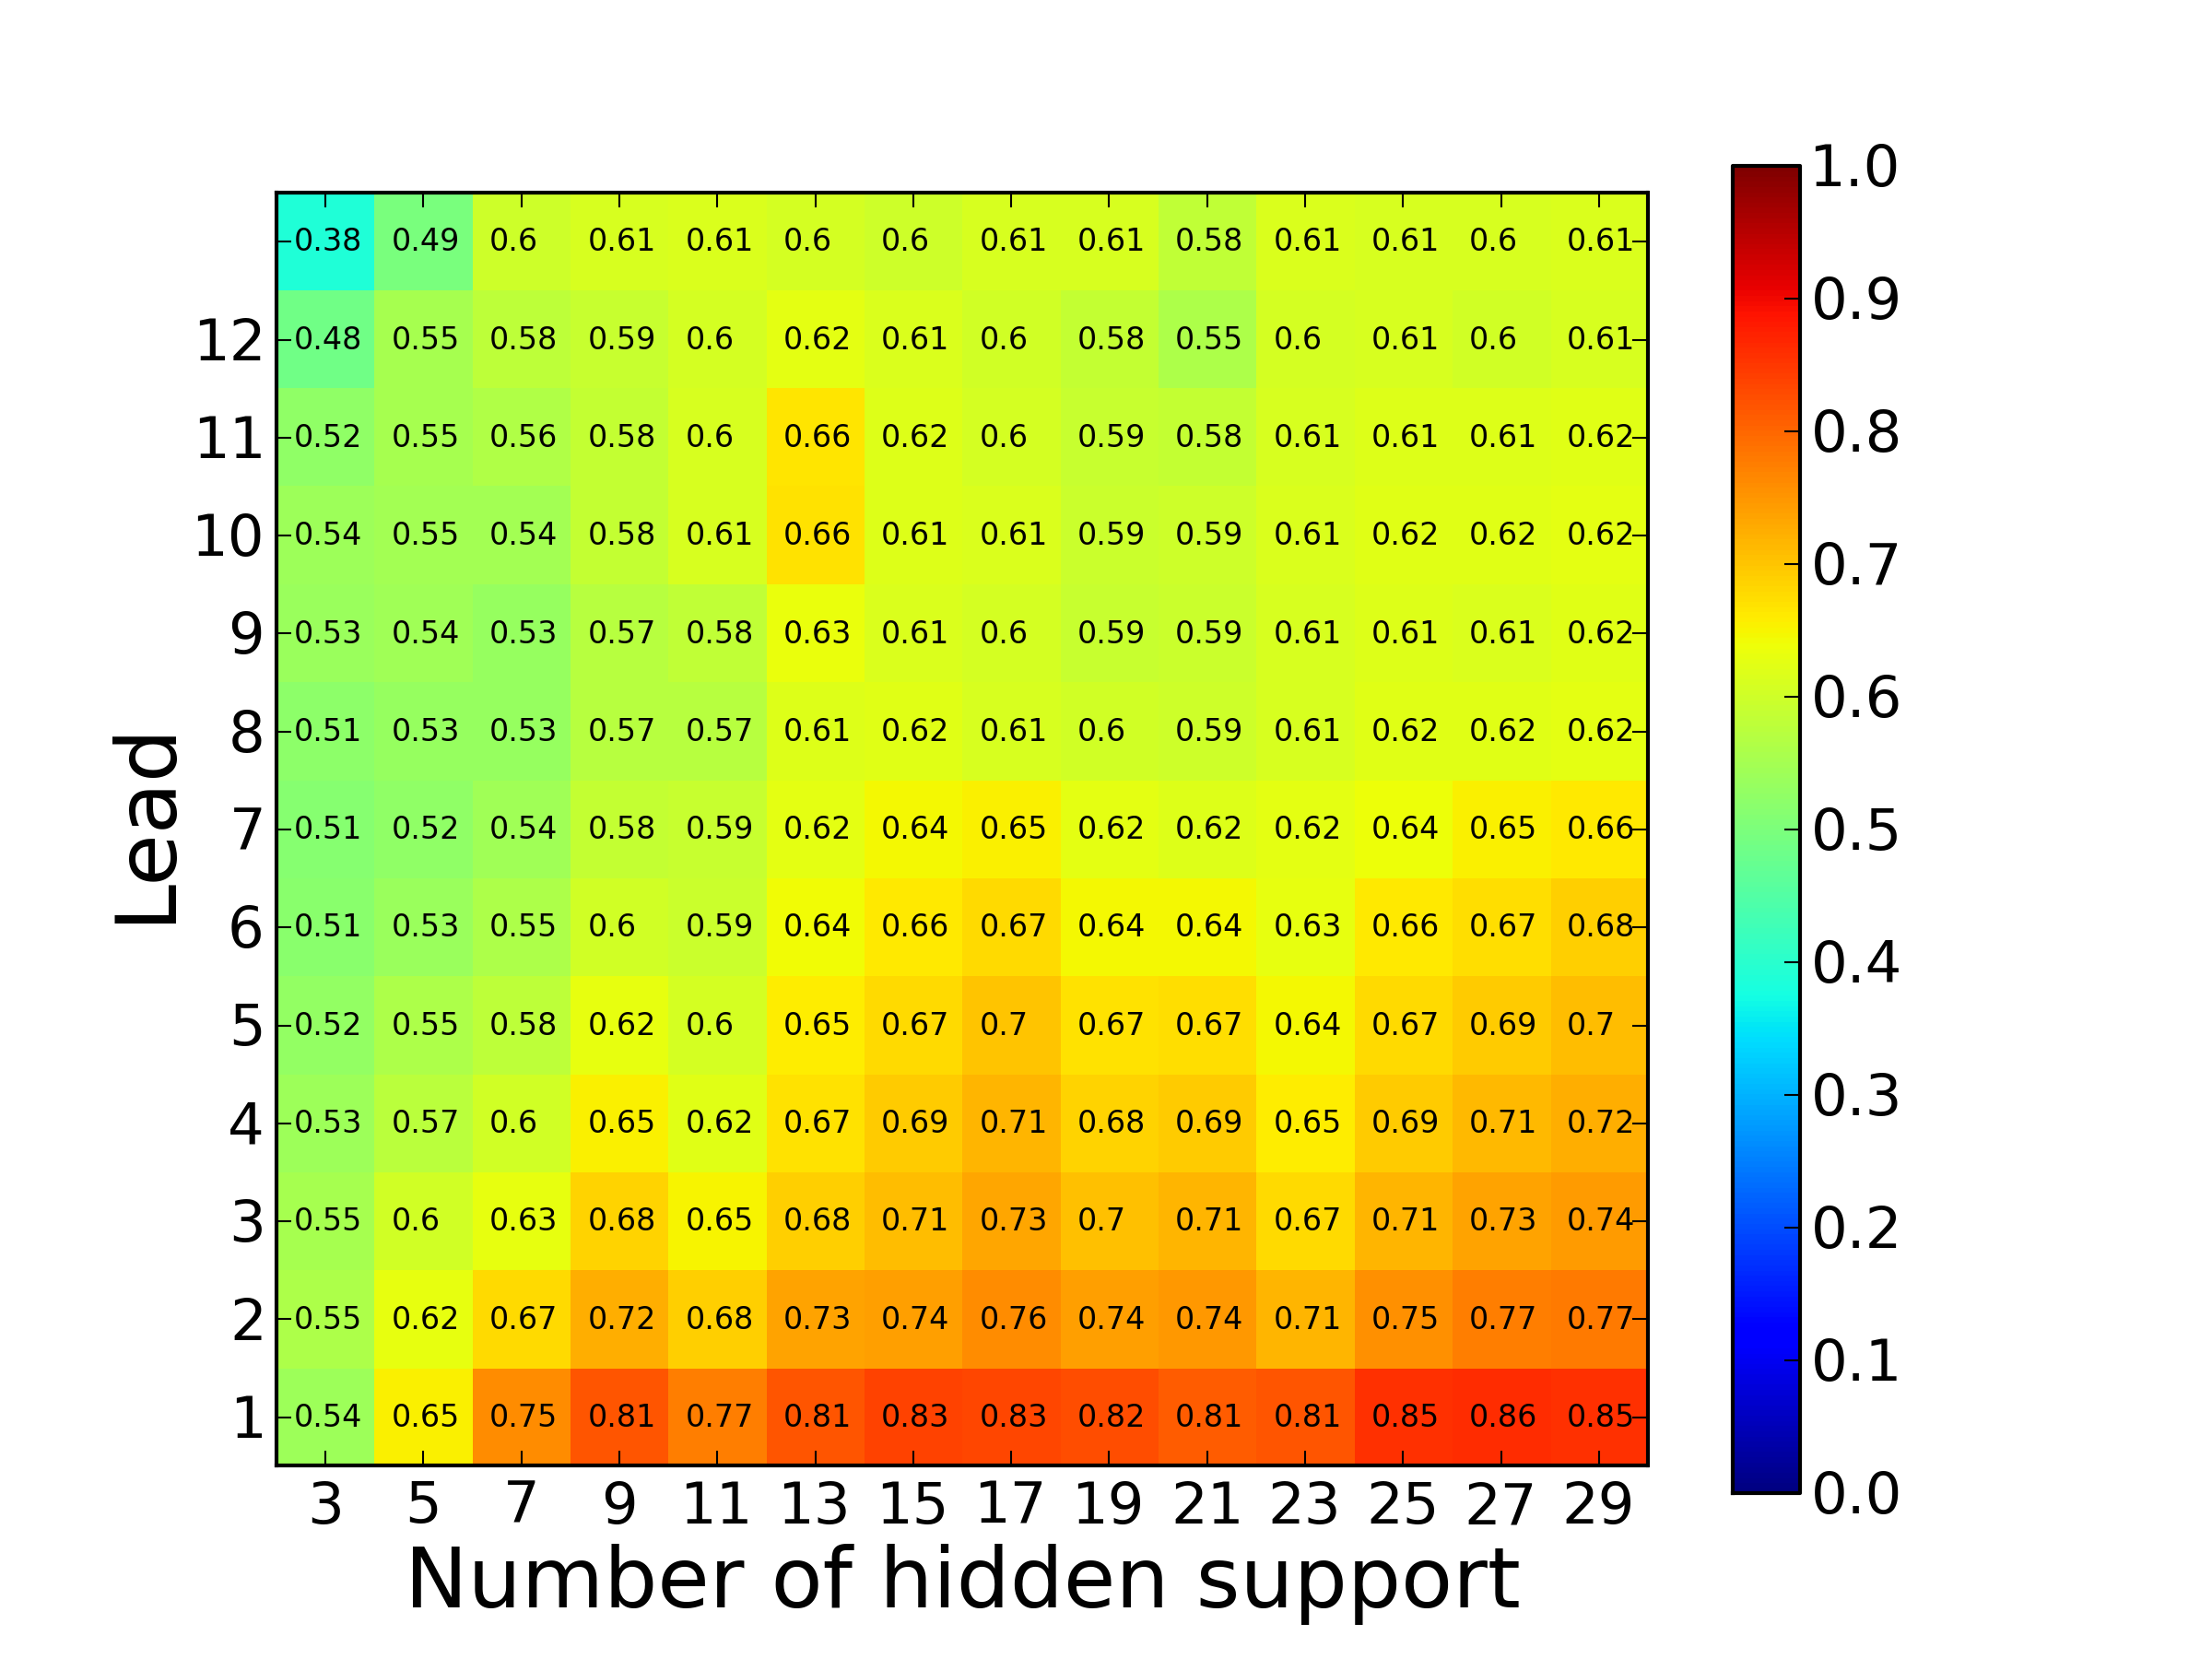
\includegraphics[width=1.0\textwidth]{figures/hmm/no_collab_pca.png}
\end{figure}

\begin{figure}[ht!]
  \caption{Heatmap for the \forum cohort. PCA transformations of features used.}\label{fig:hmm_heatmap_forum_only_pca}
  \centering
    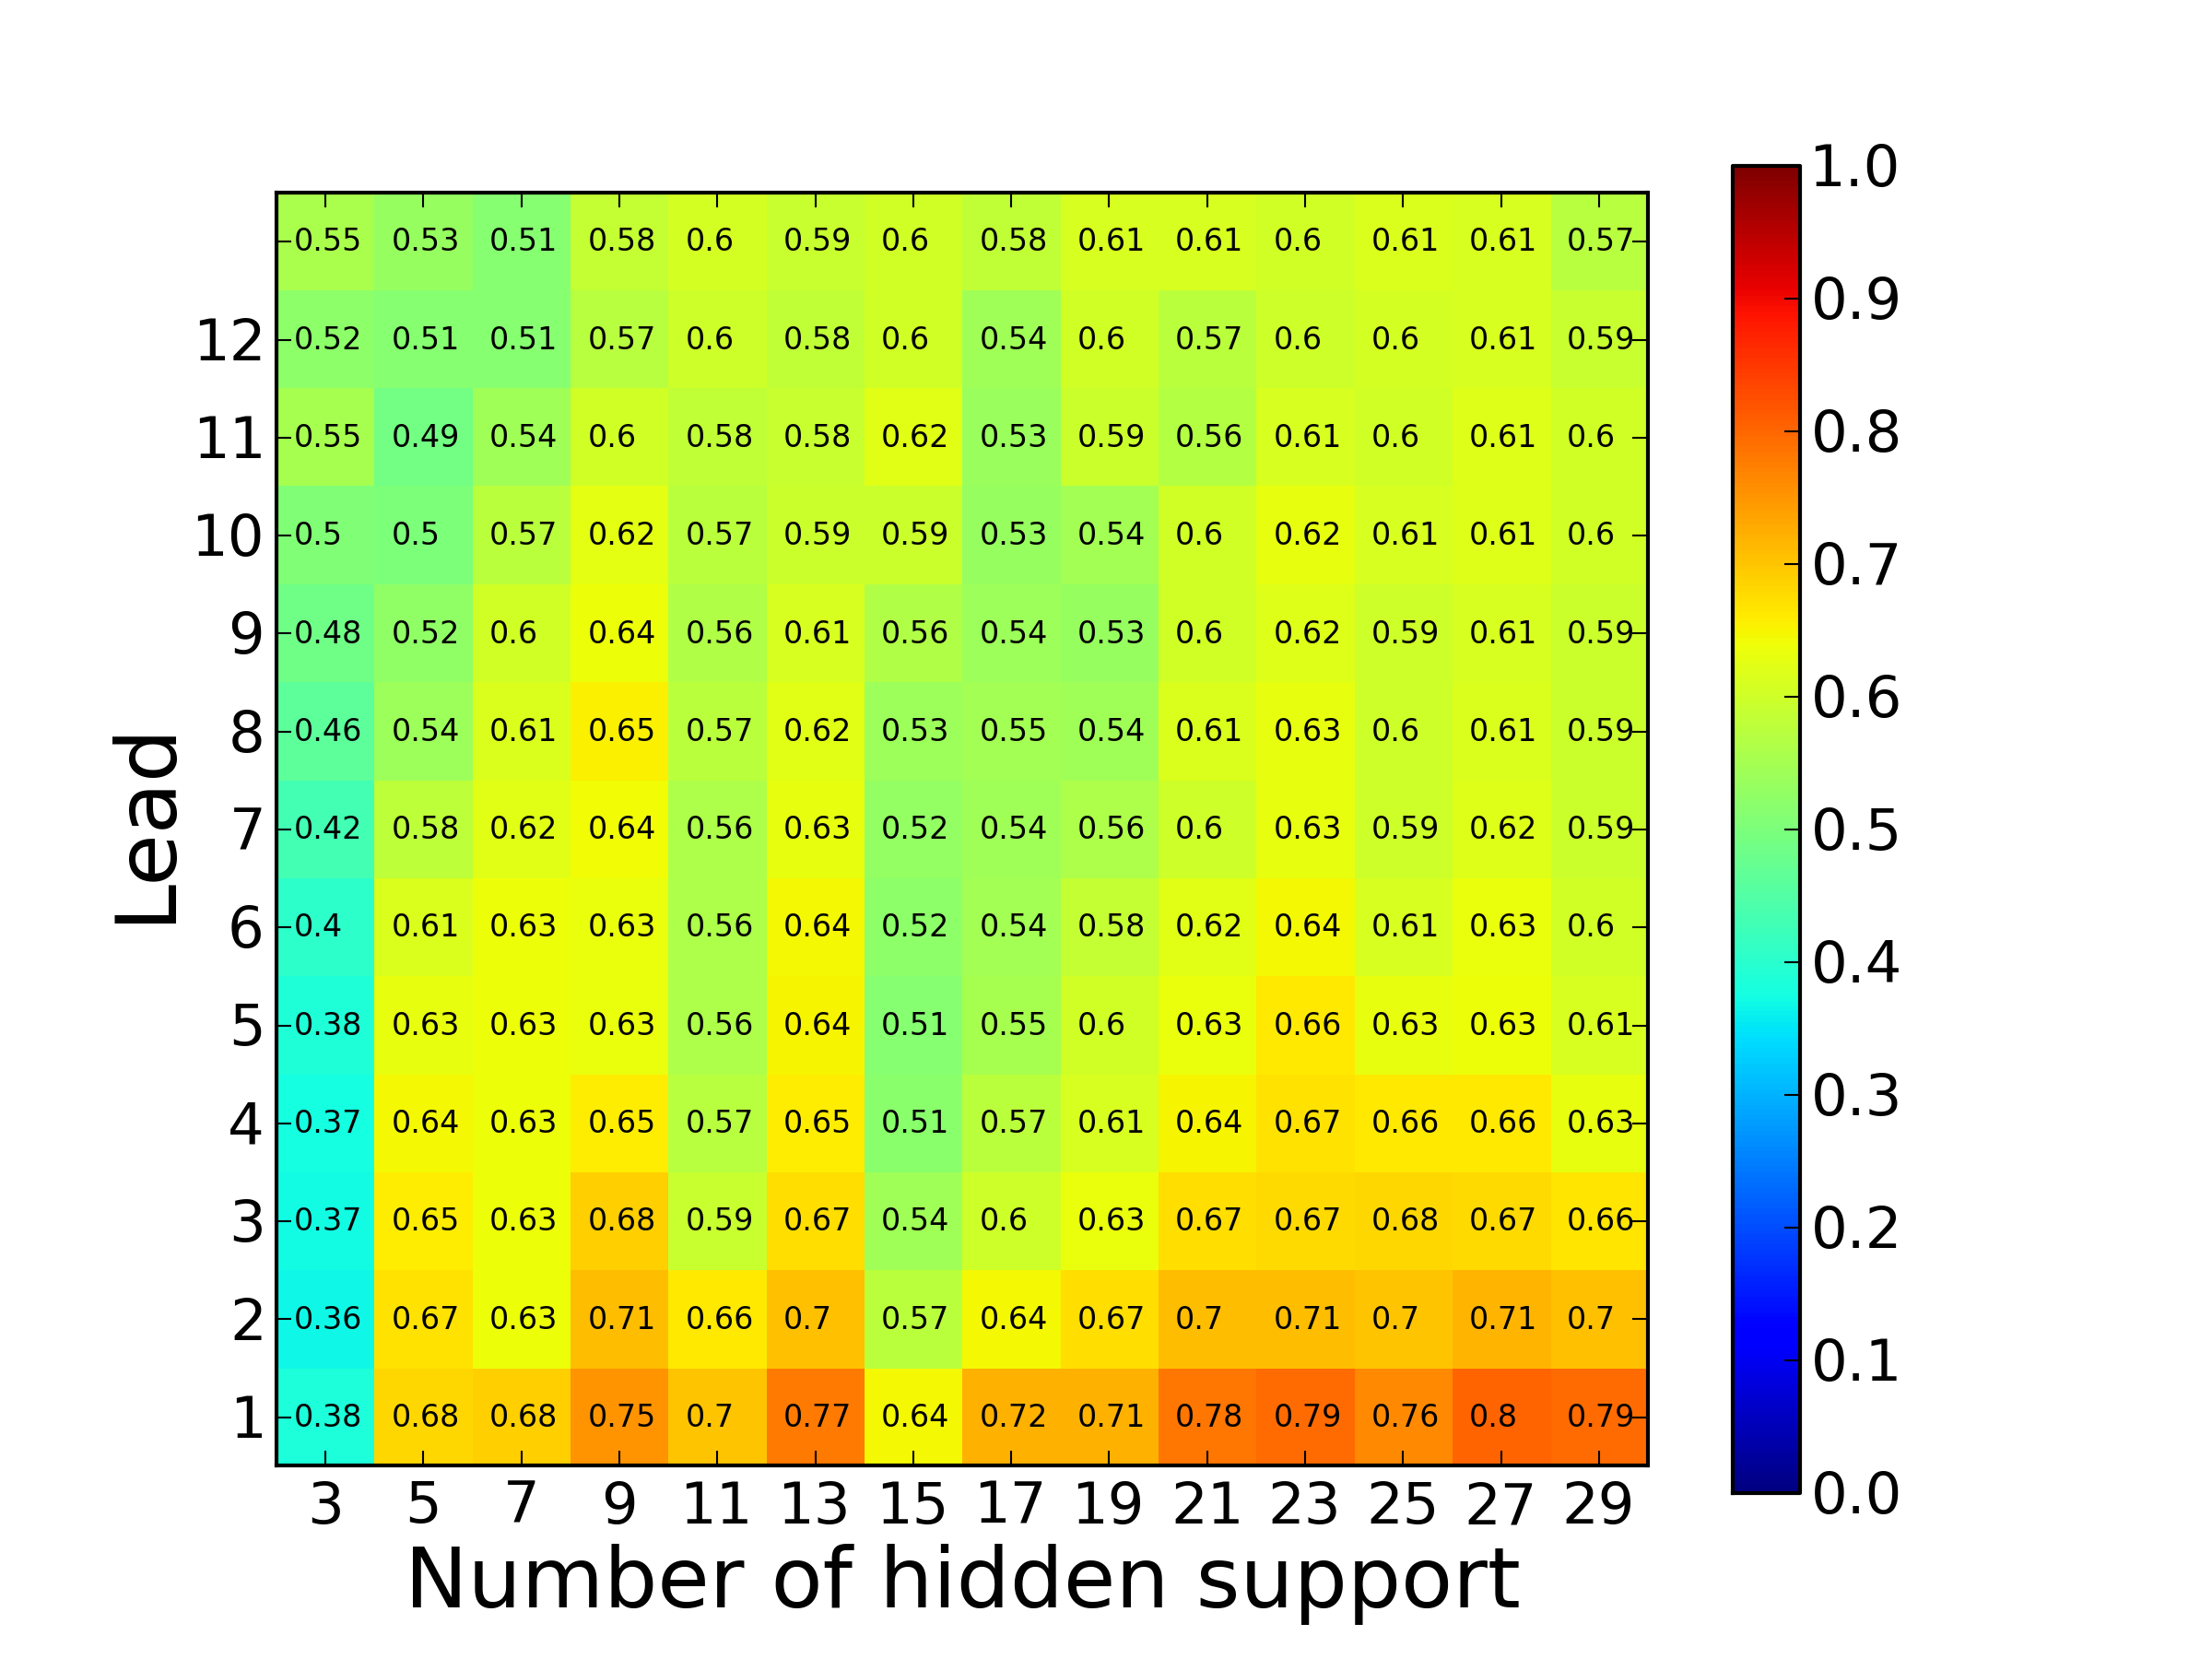
\includegraphics[width=1.0\textwidth]{figures/hmm/forum_only_pca.png}
\end{figure}

\begin{figure}[ht!]
  \caption{Heatmap for the \both cohort. PCA transformations of features used.}\label{fig:hmm_heatmap_forum_and_wiki_pca}
  \centering
    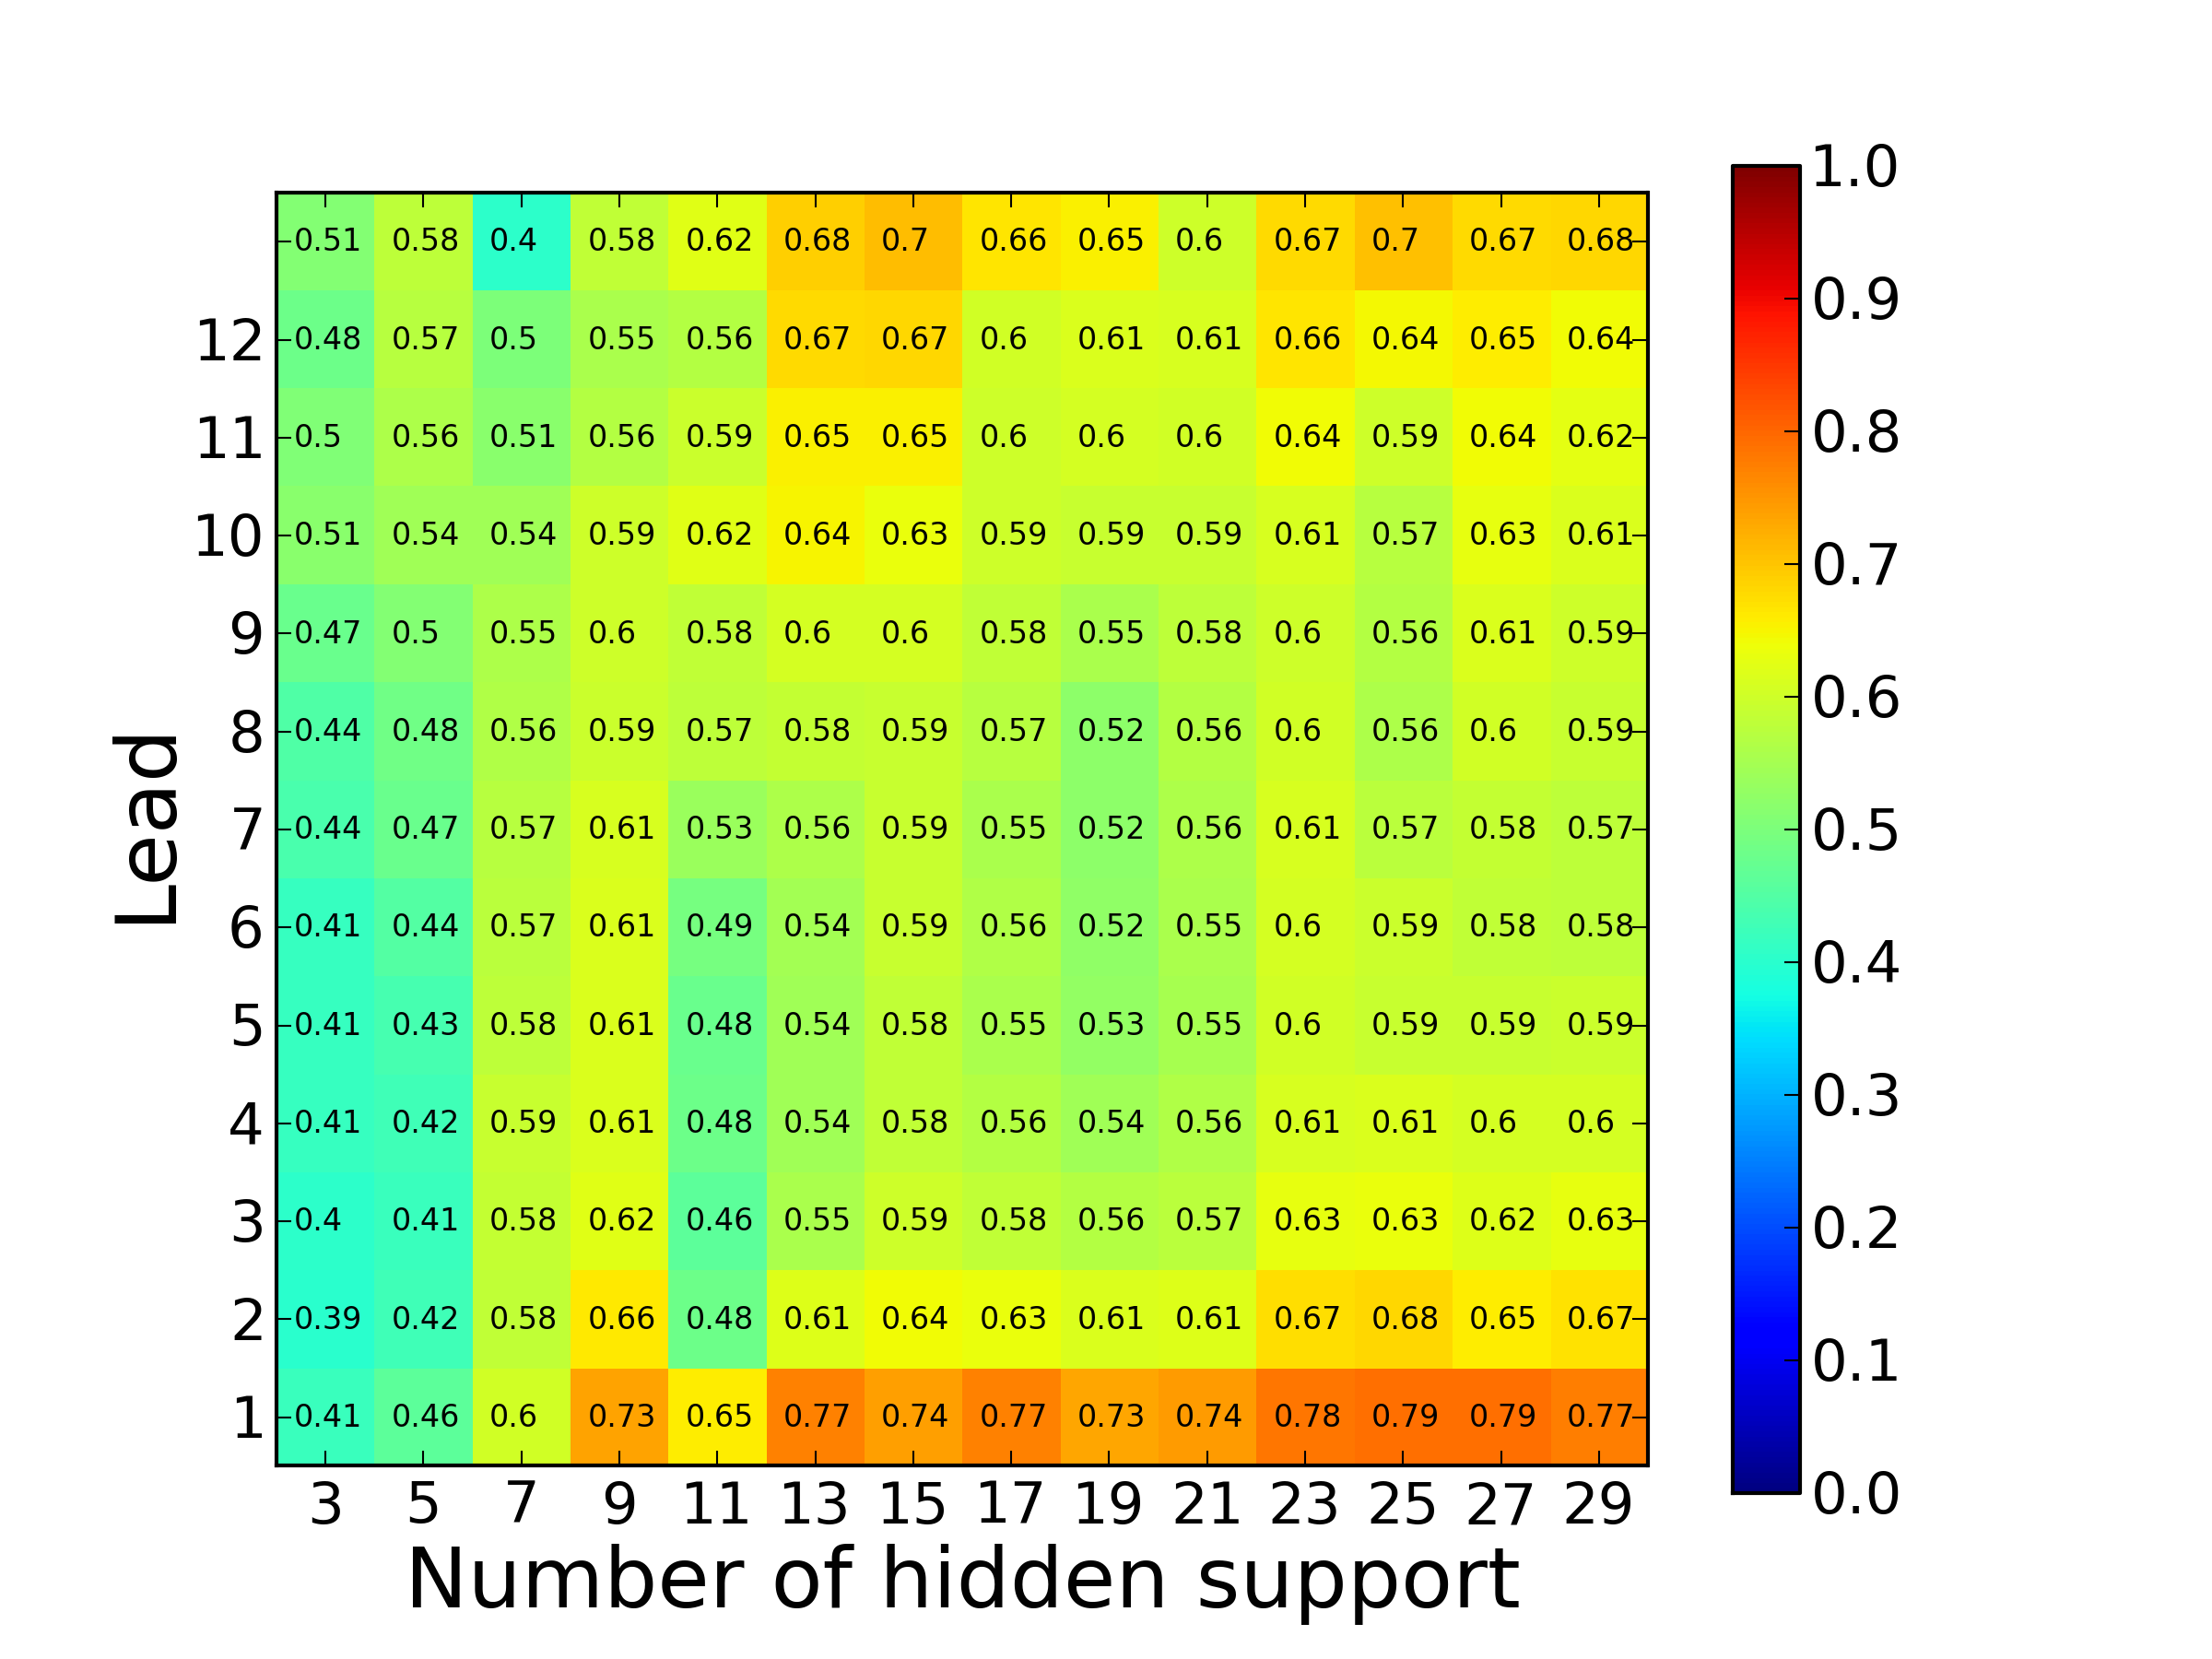
\includegraphics[width=1.0\textwidth]{figures/hmm/forum_and_wiki_pca.png}
\end{figure}

Figures \ref{fig:hmm_heatmap_no_collab_pca} to \ref{fig:hmm_heatmap_forum_and_wiki_pca} show HMM heatmaps for cohorts \neither, \forum and \both. These featuresets used PCA to reduce their dimensionality. We were unable to use PCA to reduce the \wiki cohort because it was too small. Each heatmap visualizes the ROC AUC for various leads as we vary K to create different models.

The PCA HMM models require a relatively larger K value in order to converge to a high AUC. For the \neither cohort, for example, we see that increasing K continually increases AUCs for all leads, up through a K of 29. This suggests that there are even more than 29 modes of students, and that we could attain even better results through a higher K value. The PCA HMMs show a large contrast between high leads and low leads. However, as compared with logistic regression, we see more consistent results cross the cohorts. For example, with a lead of one, the \neither, \forum and \both cohorts are within 0.08 of each other. In logistic regression, there is a difference in AUC of 0.2.

We suspect that the high difference in predictive accuracies between high leads and low leads is due to the fact that HMMs use a single transition matrix for all weeks. There is likely to be different probabilities of transferring hidden state between weeks 1 and 2 than between 12 and 13, for example, but the HMM posits only one set of probabilities. Furthermore, since there are more students in earlier weeks due to stopout, the transition matrix will have more examples from earlier weeks. Thus, it will be biased towards the earlier weeks, allowing for better prediction in the earlier weeks than in later weeks. 

\begin{figure}[ht!]
  \caption{Mean AUC as K increases for the \neither cohort. PCA transformations of features used.}\label{fig:hmm_support_over_time_no_collab_pca}
  \centering
    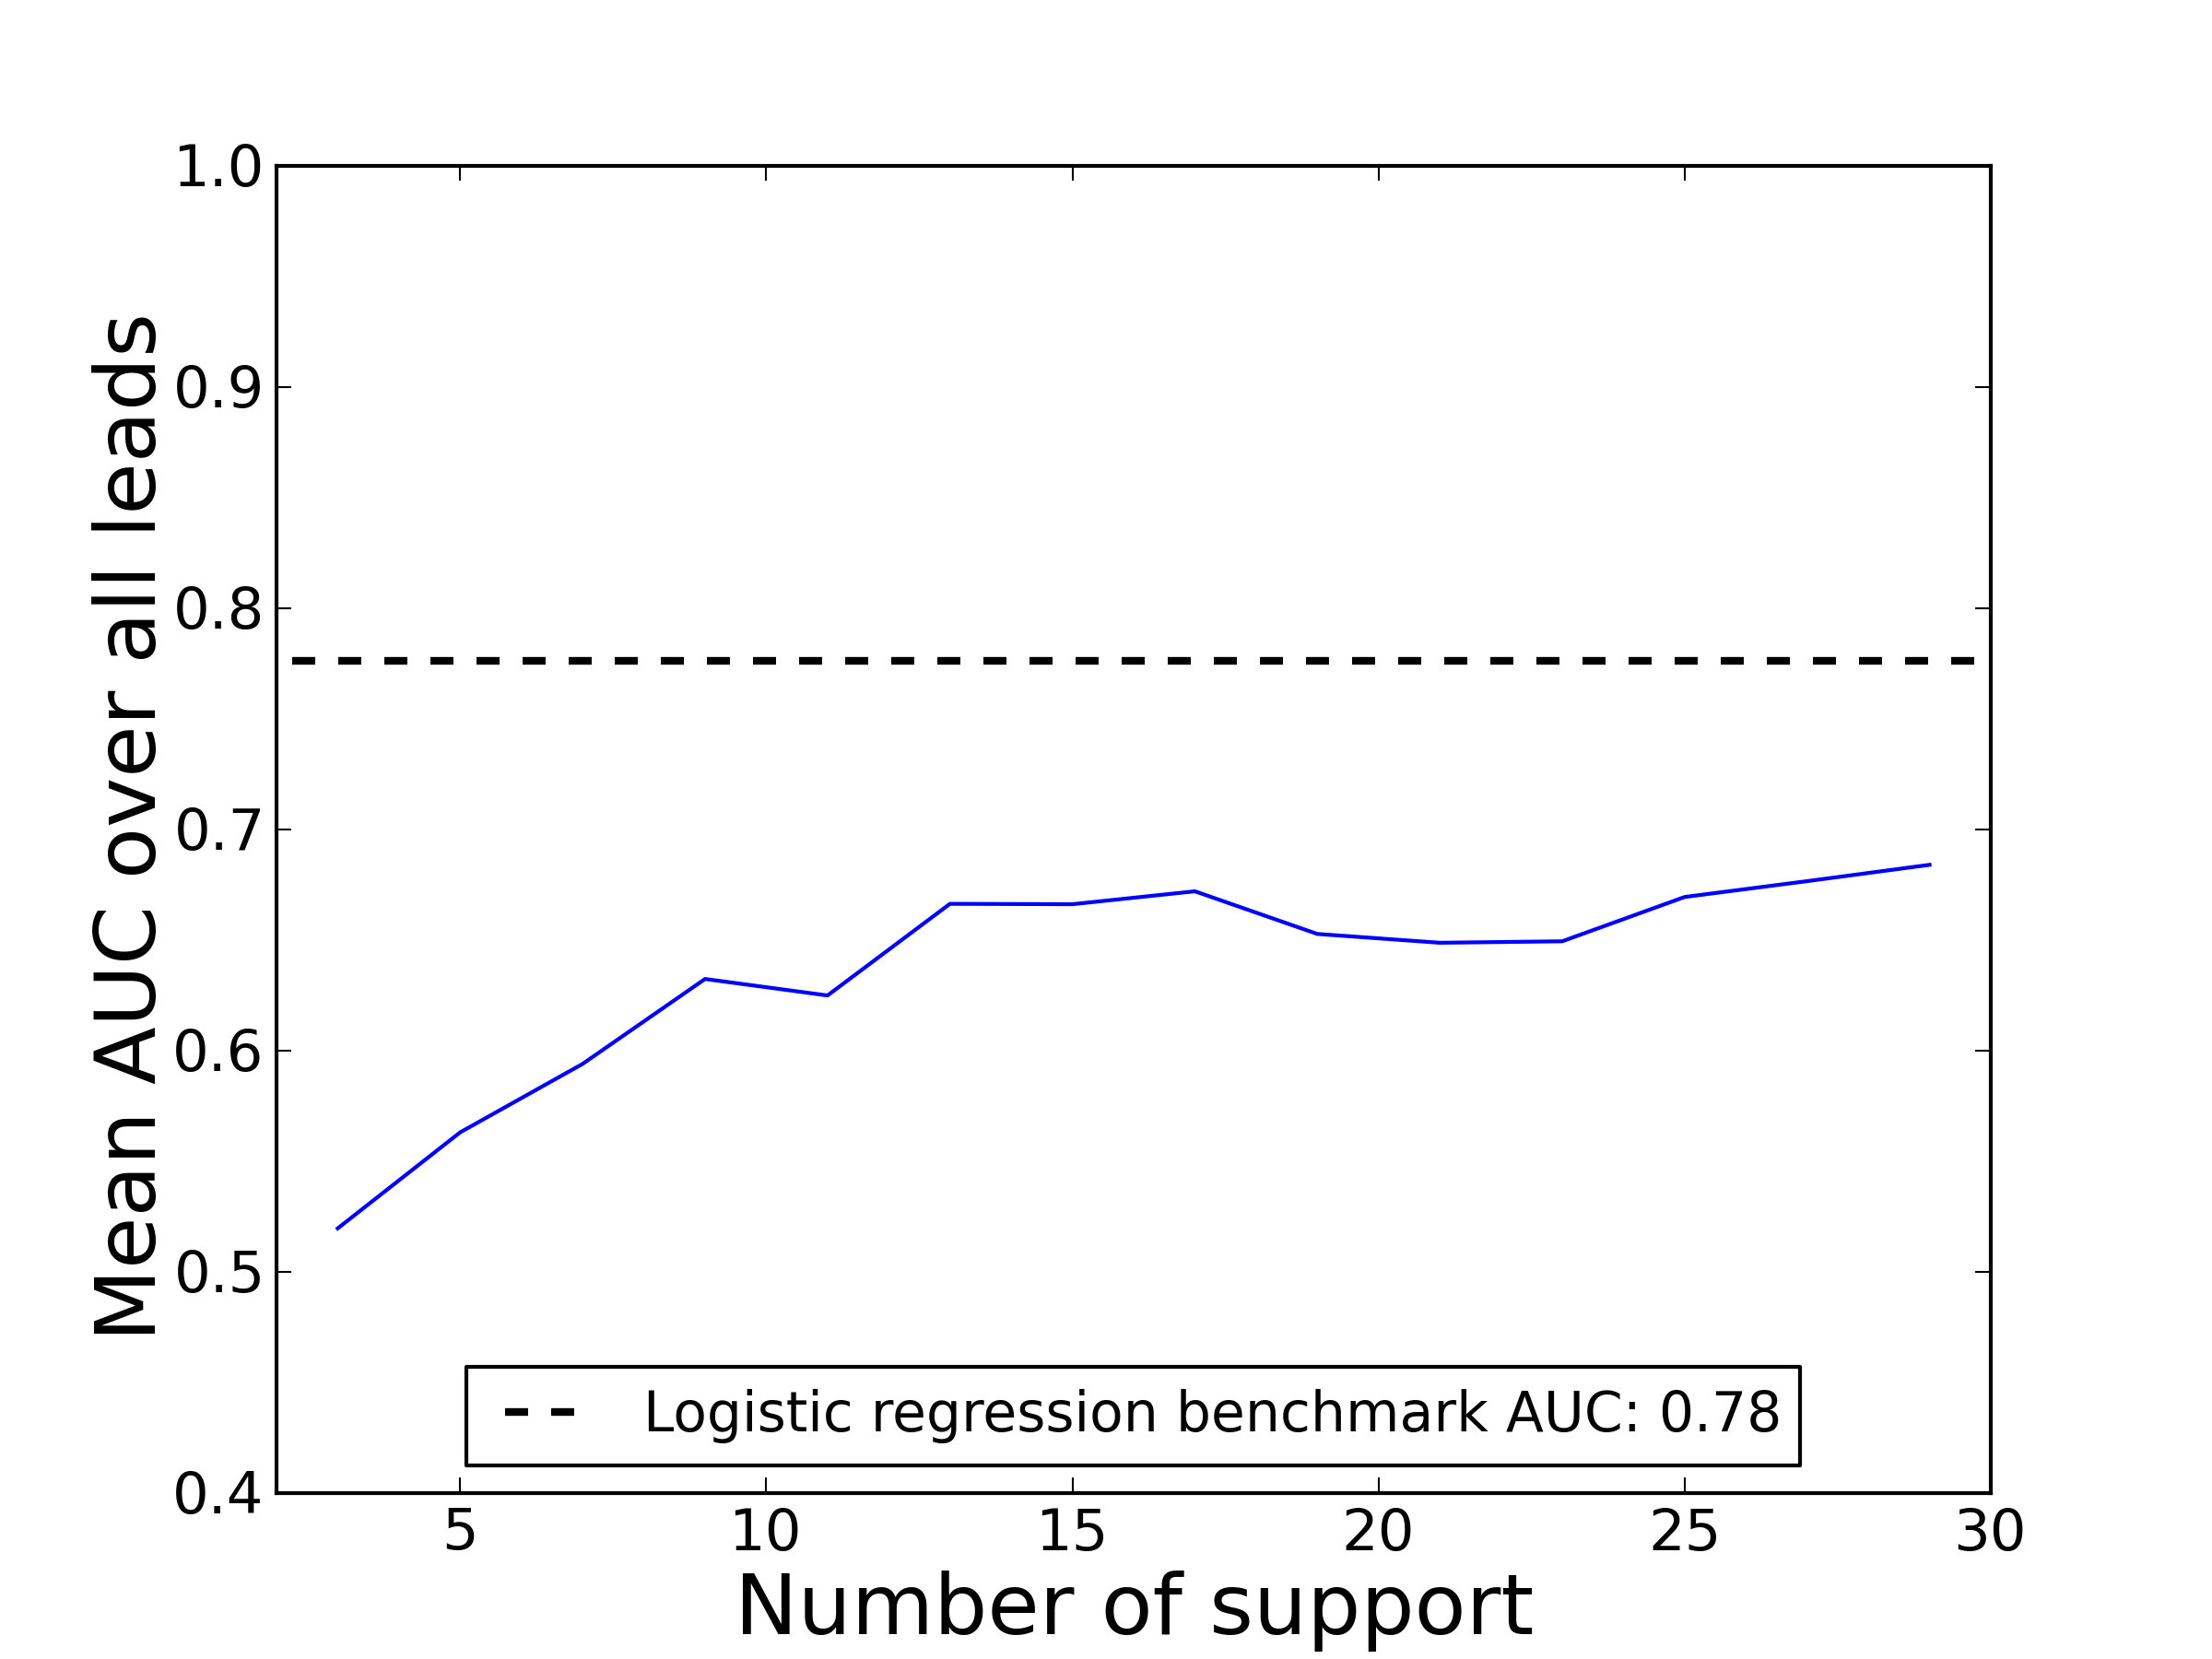
\includegraphics[width=0.8\textwidth]{figures/hmm/no_collab_pca_support_over_time.png}
\end{figure}

\begin{figure}[ht!]
  \caption{Mean AUC as K increases for the \forum cohort. PCA transformations of features used.}\label{fig:hmm_support_over_time_forum_only_pca}
  \centering
    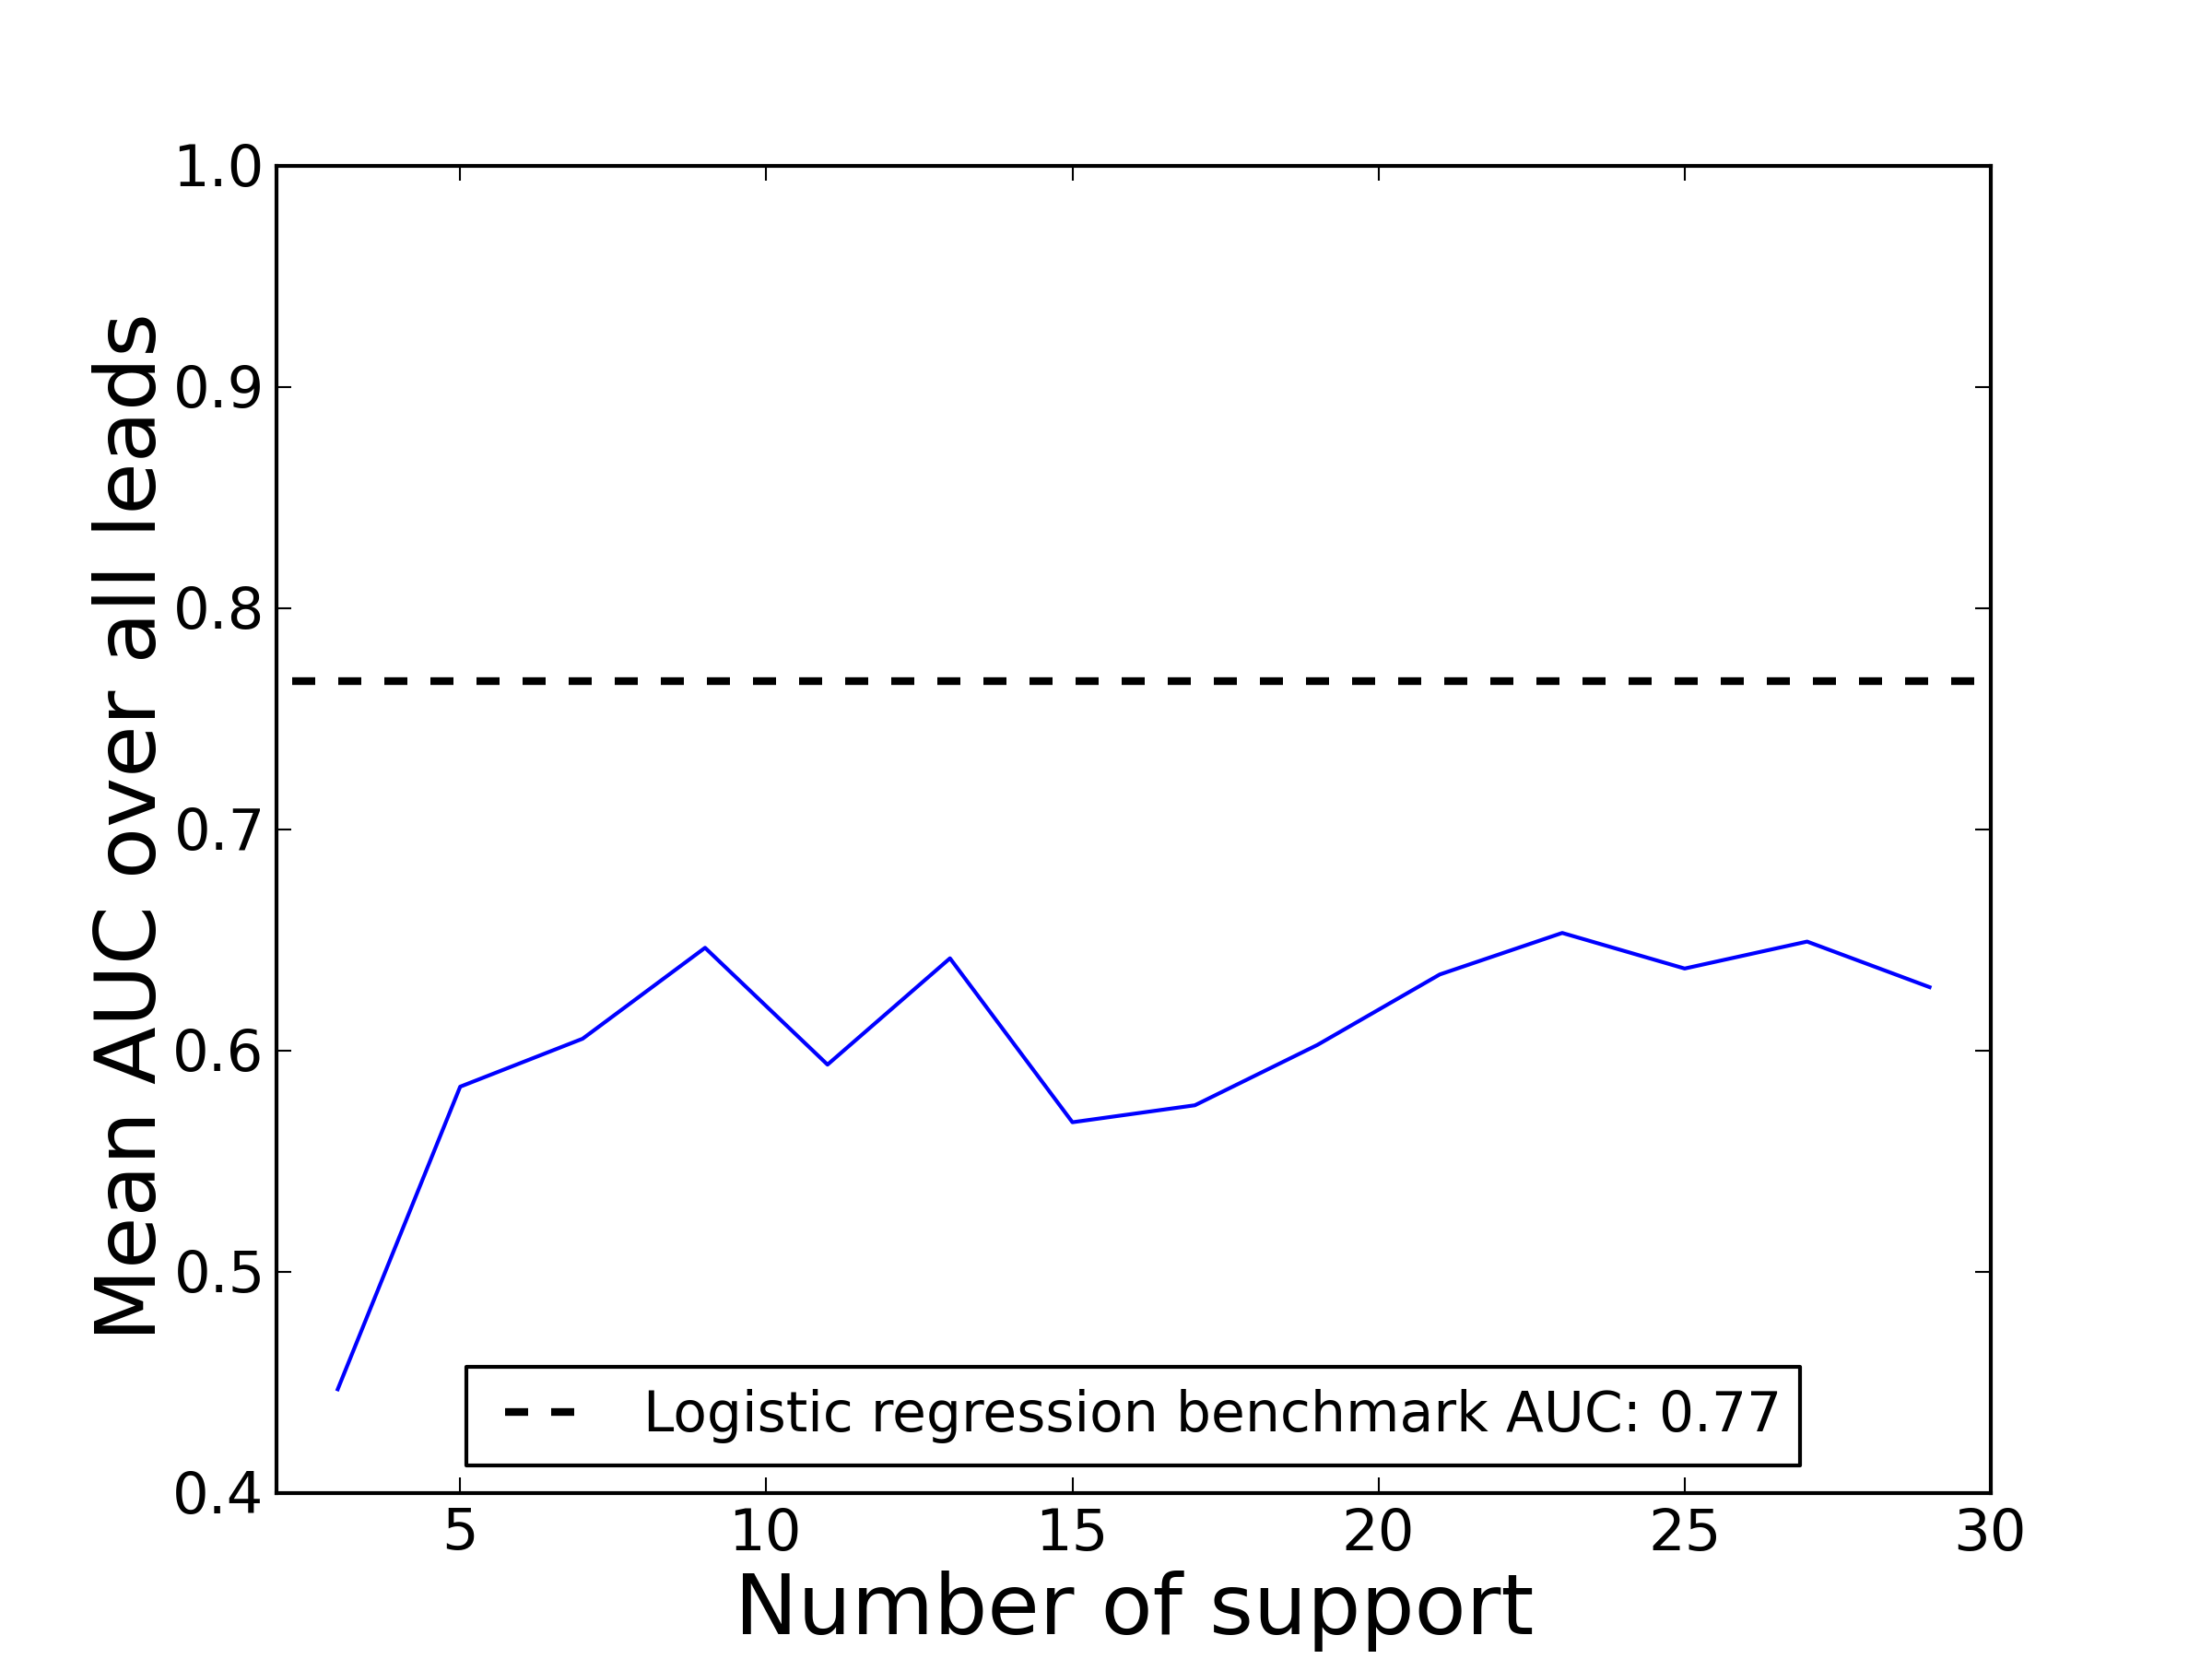
\includegraphics[width=0.8\textwidth]{figures/hmm/forum_only_pca_support_over_time.png}
\end{figure}

\begin{figure}[ht!]
  \caption{Mean AUC as K increases for the \both cohort. PCA transformations of features used.}\label{fig:hmm_support_over_time_forum_and_wiki_pca}
  \centering
    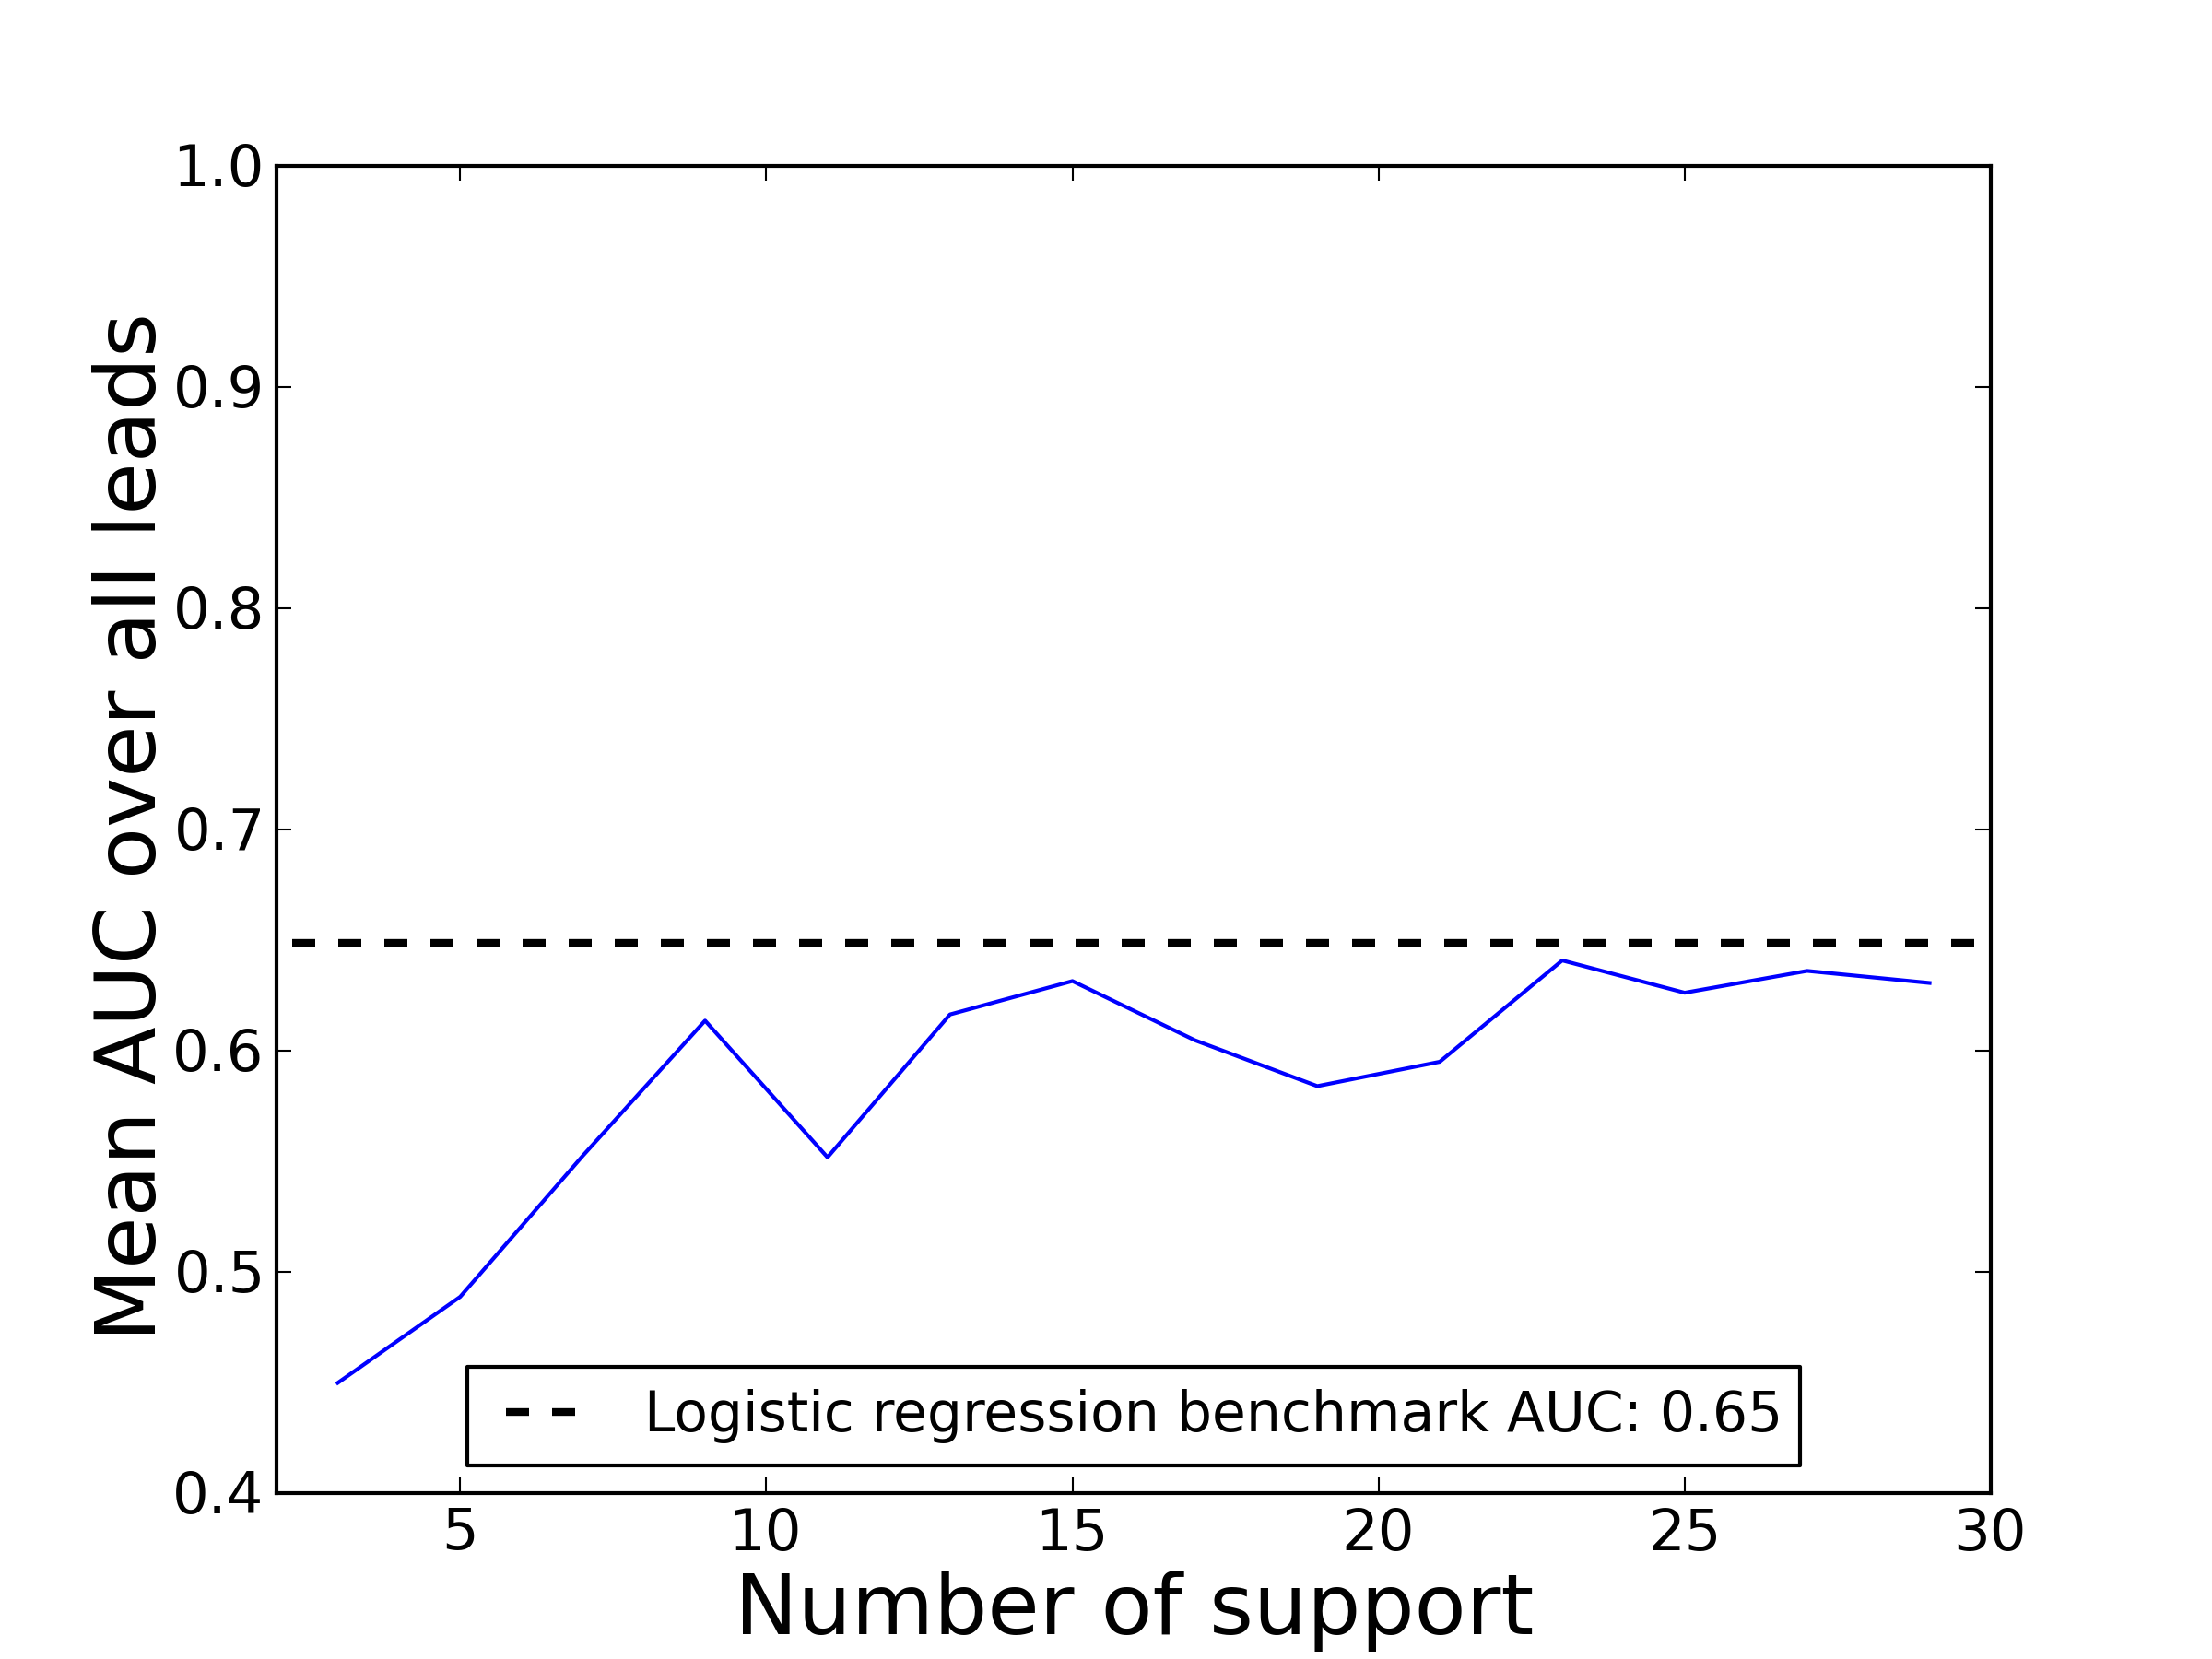
\includegraphics[width=0.8\textwidth]{figures/hmm/forum_and_wiki_pca_support_over_time.png}
\end{figure}


The following line graphs show how overall predictive accuracies of the PCA HMM models change as K increases. These graphs indicate the correct number of hidden states needed in order to model each cohort. See Figures \ref{fig:hmm_support_over_time_no_collab_pca} through 
\ref{fig:hmm_support_over_time_forum_and_wiki_pca}. The mean prediction AUC of all 91 experiments for logistic regression is also shown for each cohort as a benchmark.

The results again indicate that the \forum and \both cohorts seem to have converged, but not until K has reached ~25. However, the \neither cohort's mean AUC is still increasing as K goes to 29, indicating that a higher K could better model this cohort.

\begin{figure}[ht!]
  \caption{Heatmap for the \neither cohort.}\label{fig:hmm_heatmap_no_collab}
  \centering
    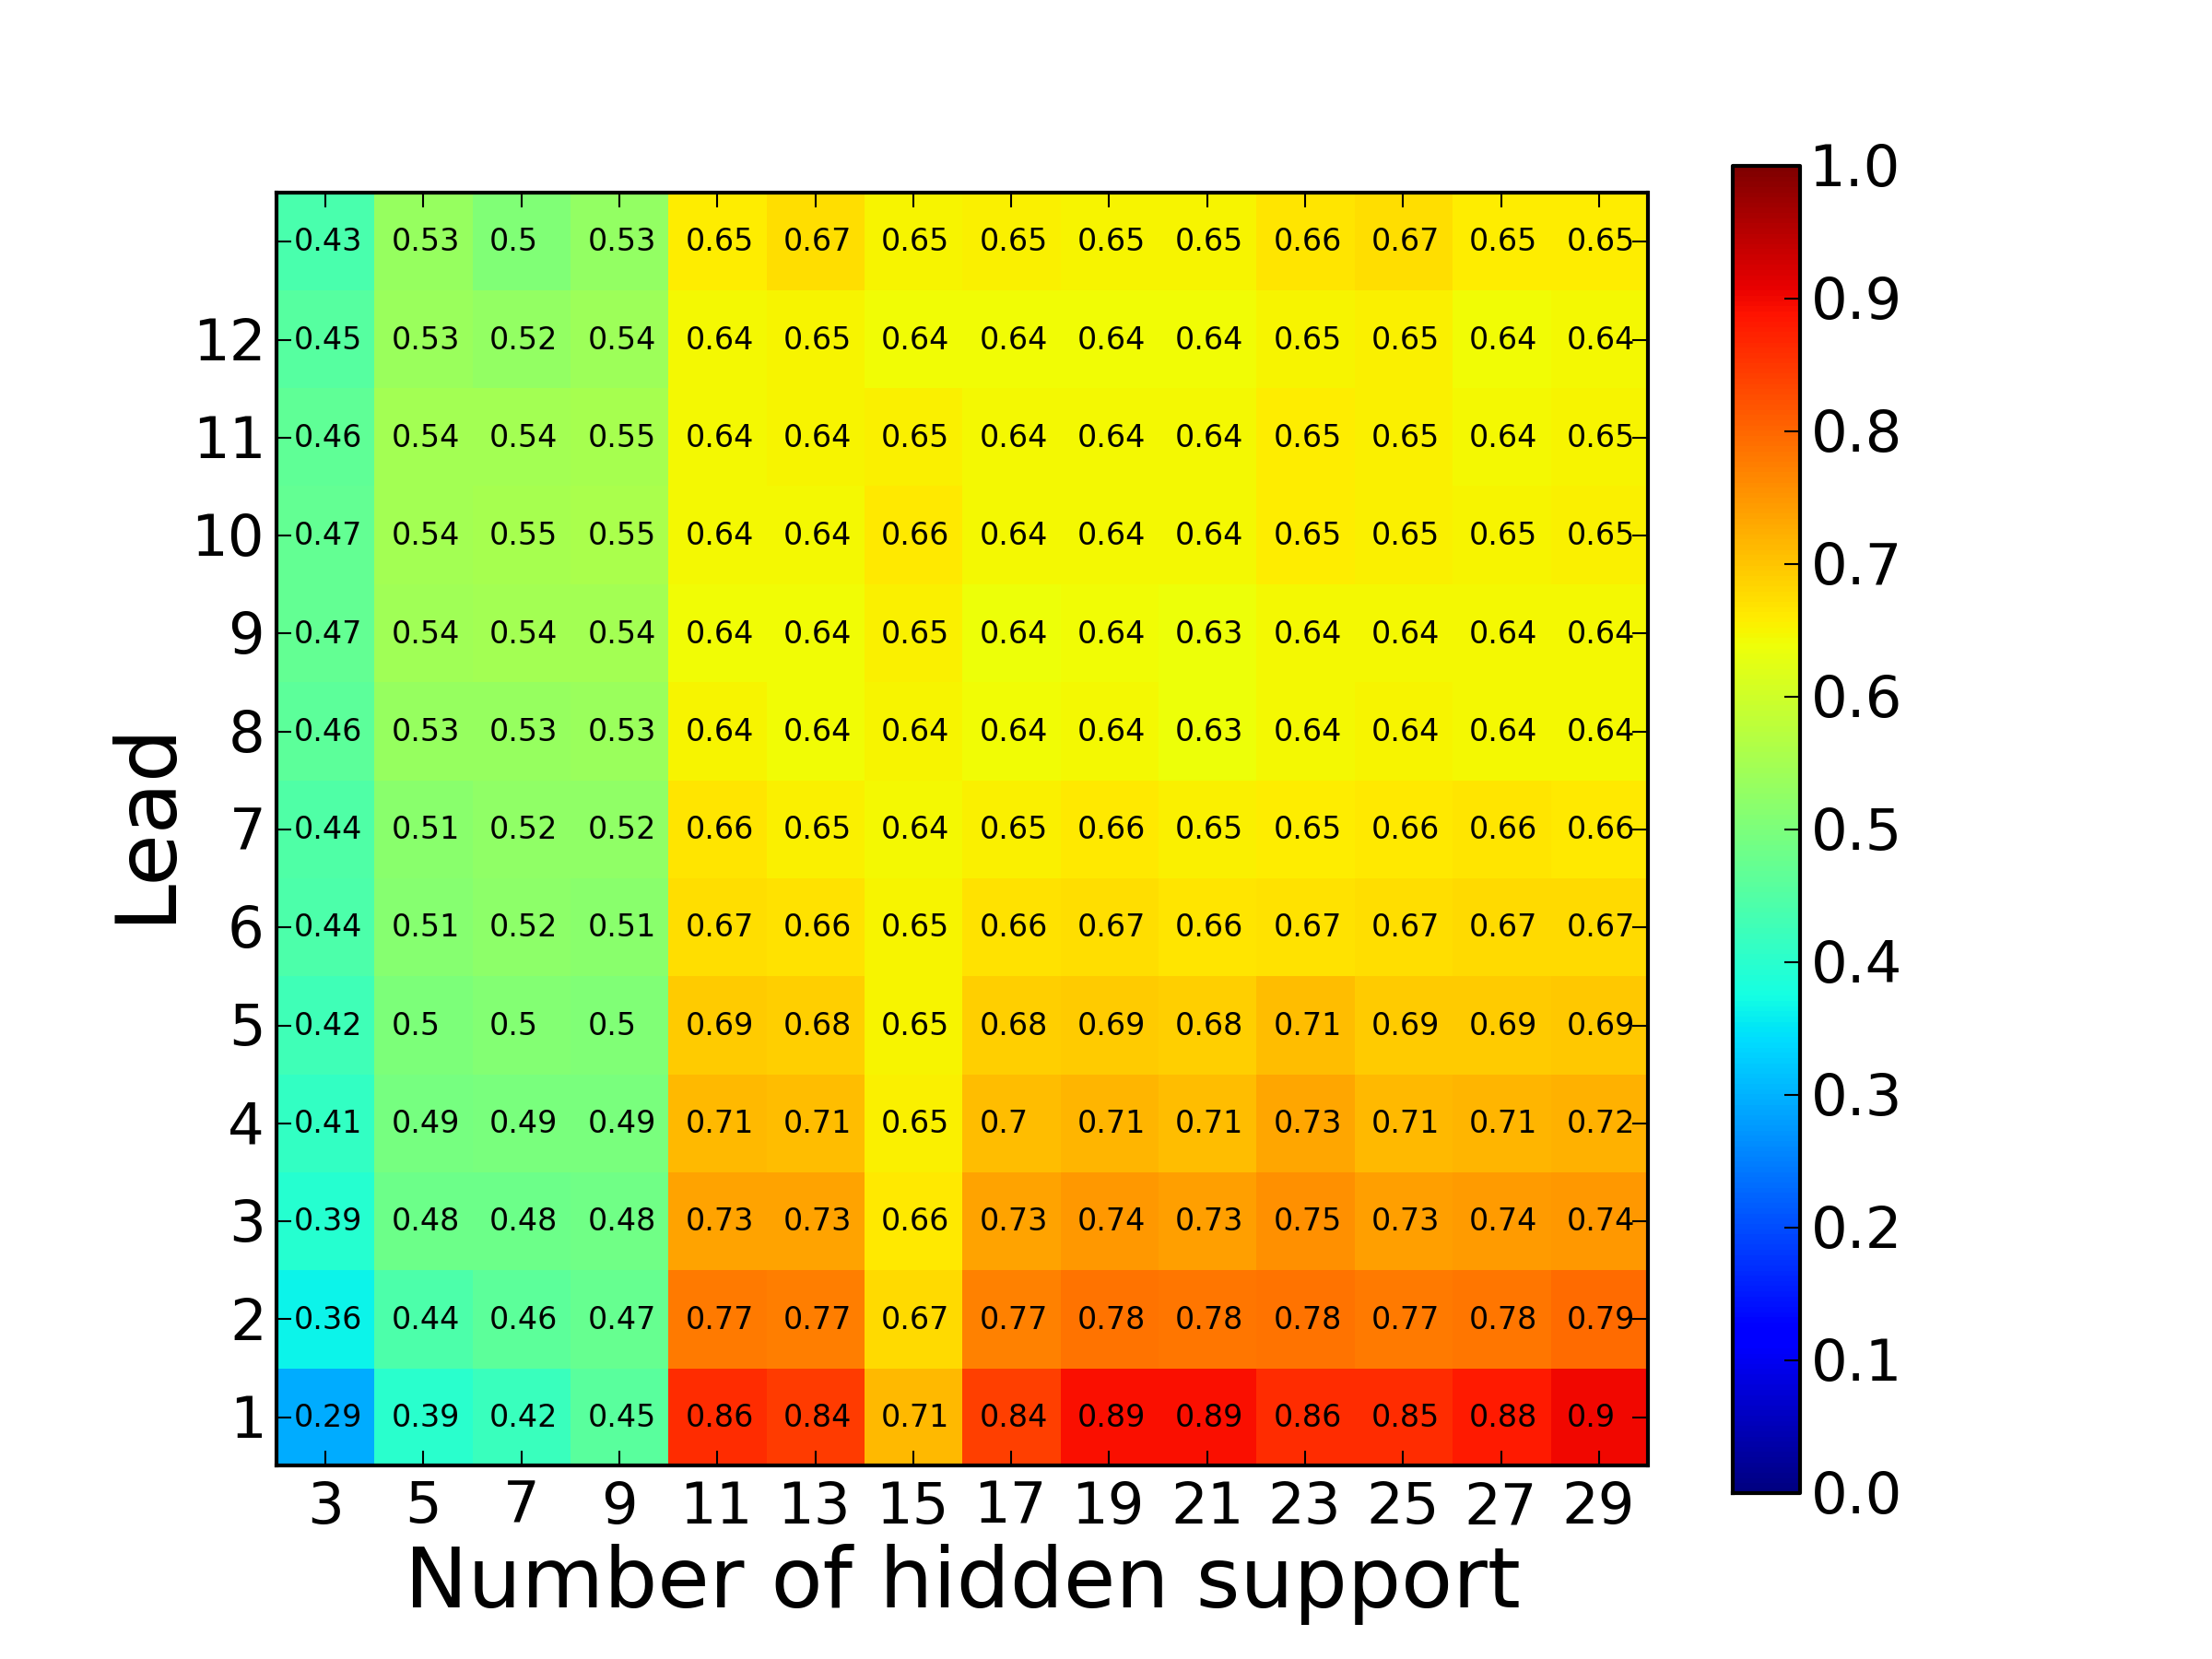
\includegraphics[width=1.0\textwidth]{figures/hmm/no_collab.png}
\end{figure}

\begin{figure}[ht!]
  \caption{Heatmap for the \forum cohort.}\label{fig:hmm_heatmap_forum_only}
  \centering
    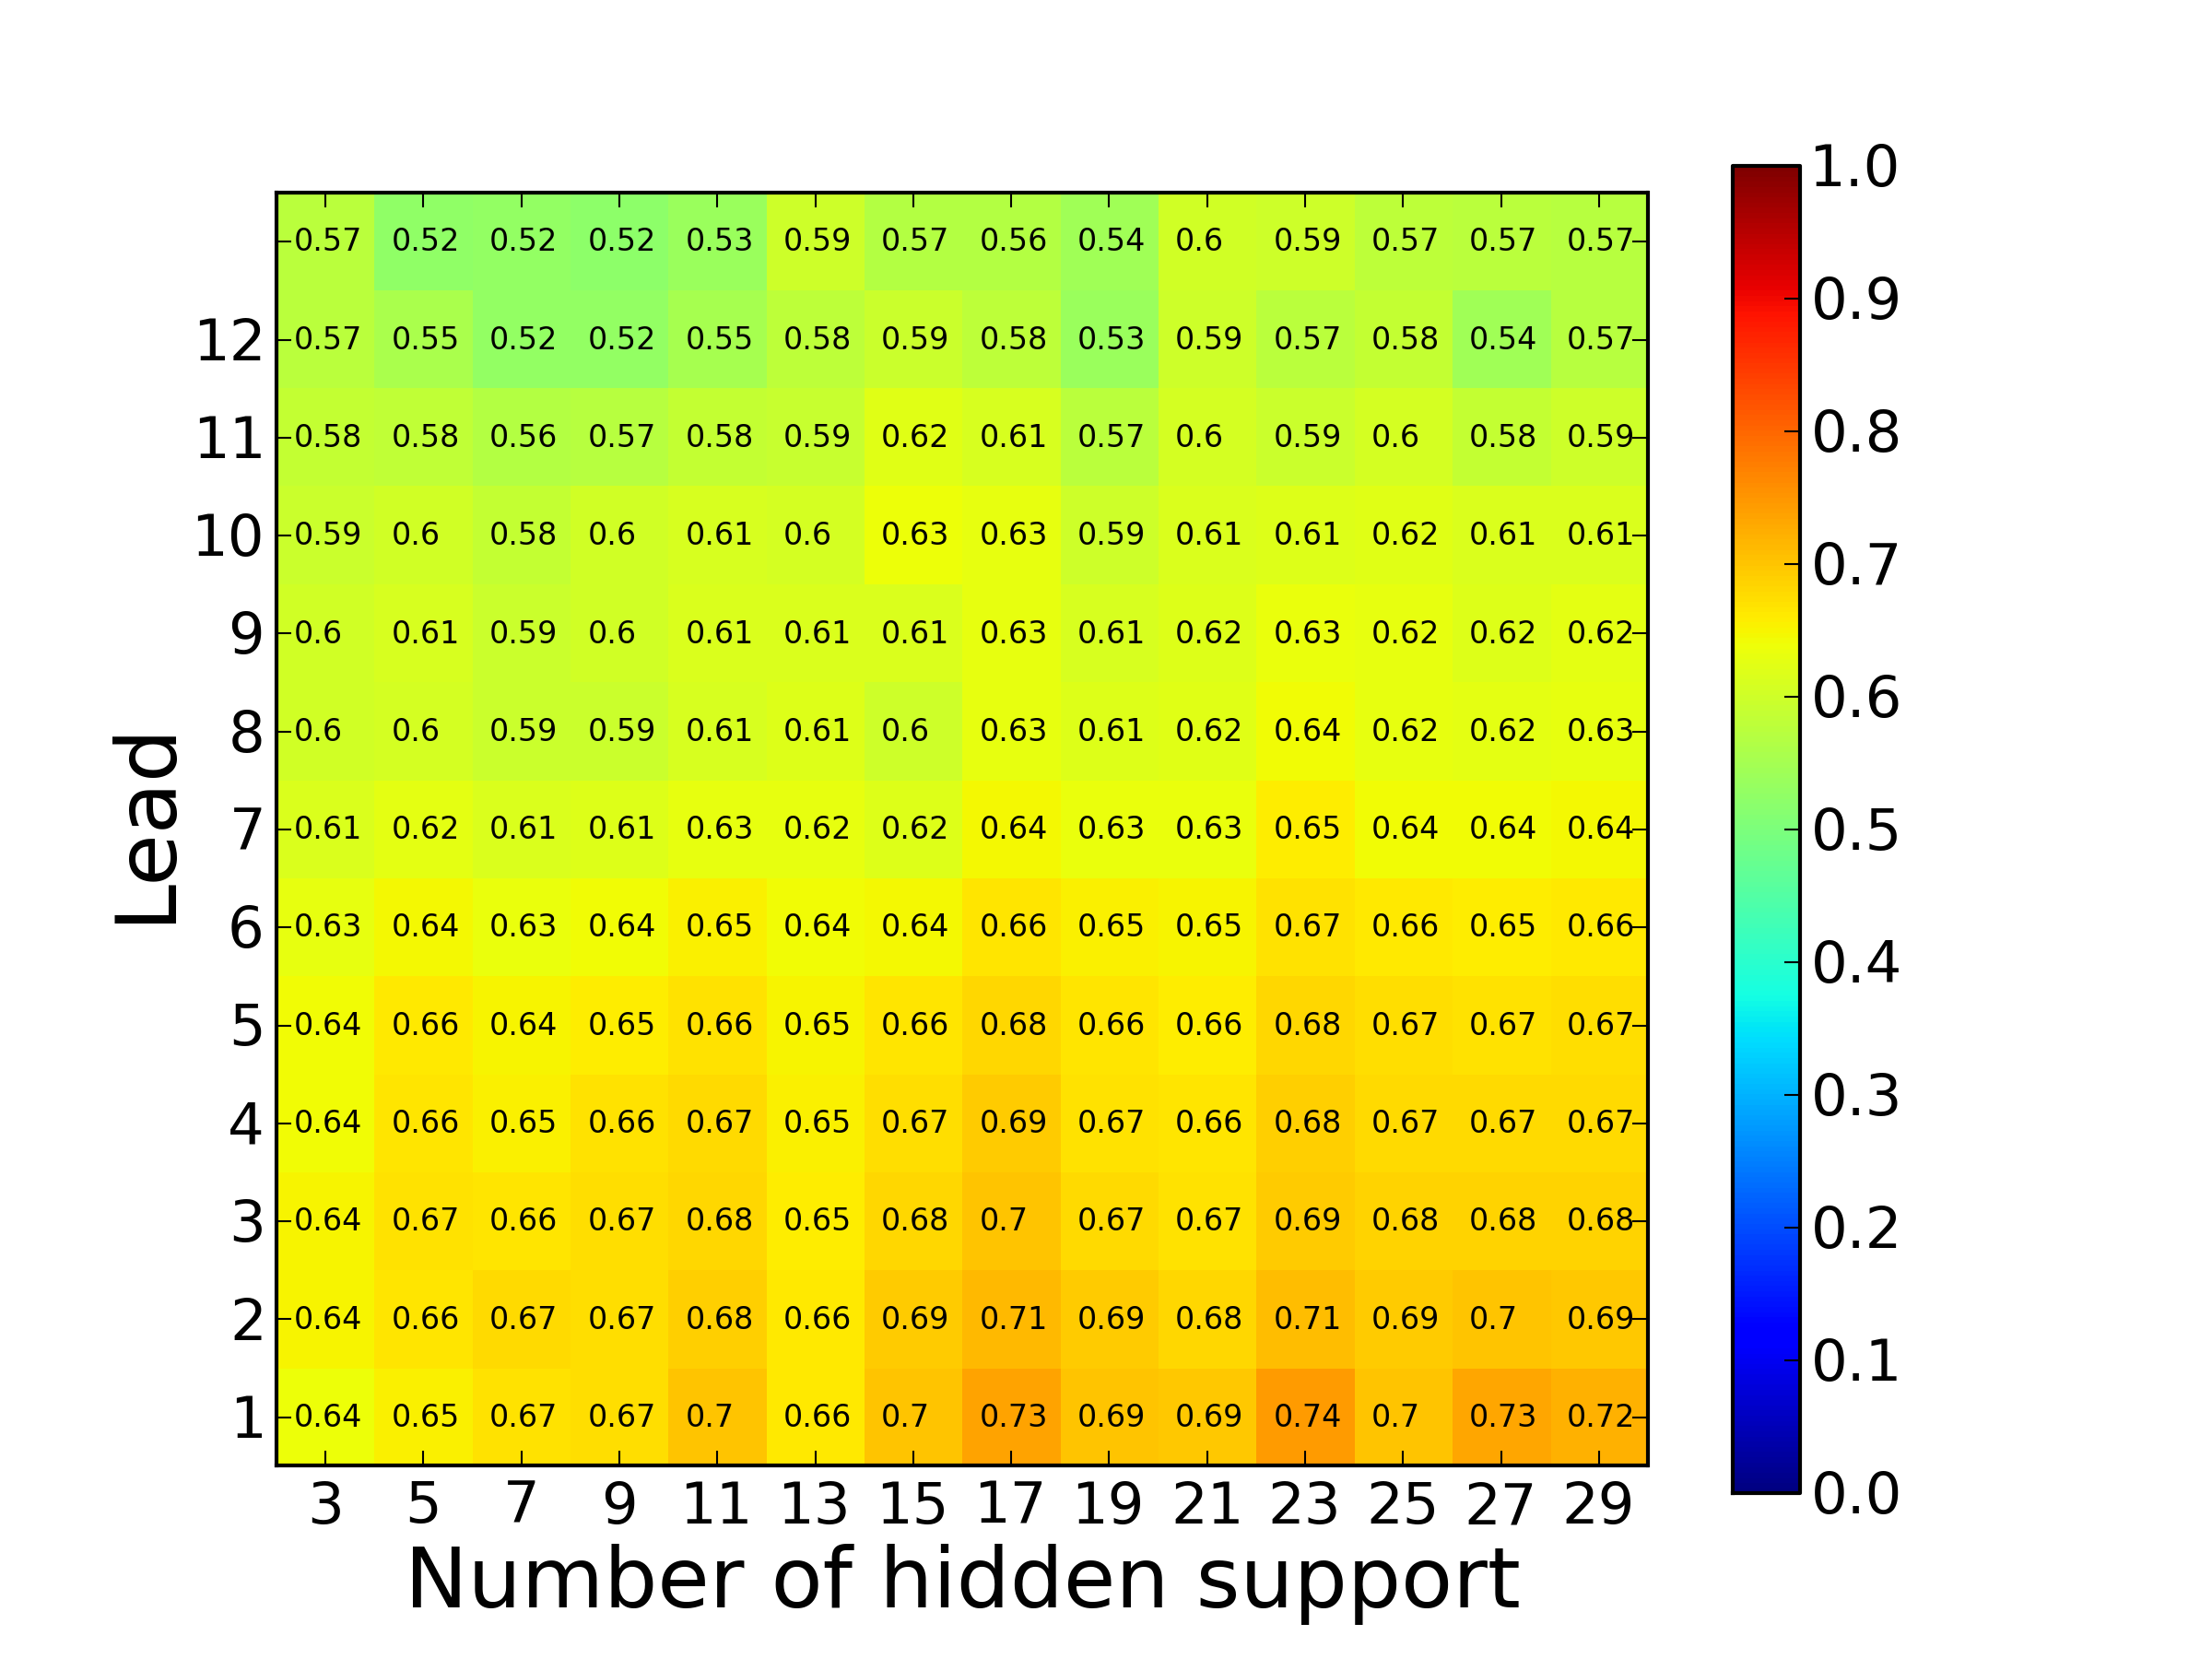
\includegraphics[width=1.0\textwidth]{figures/hmm/forum_only.png}
\end{figure}

\begin{figure}[ht!]
  \caption{Heatmap for the \both cohort.}\label{fig:hmm_heatmap_forum_and_wiki}
  \centering
    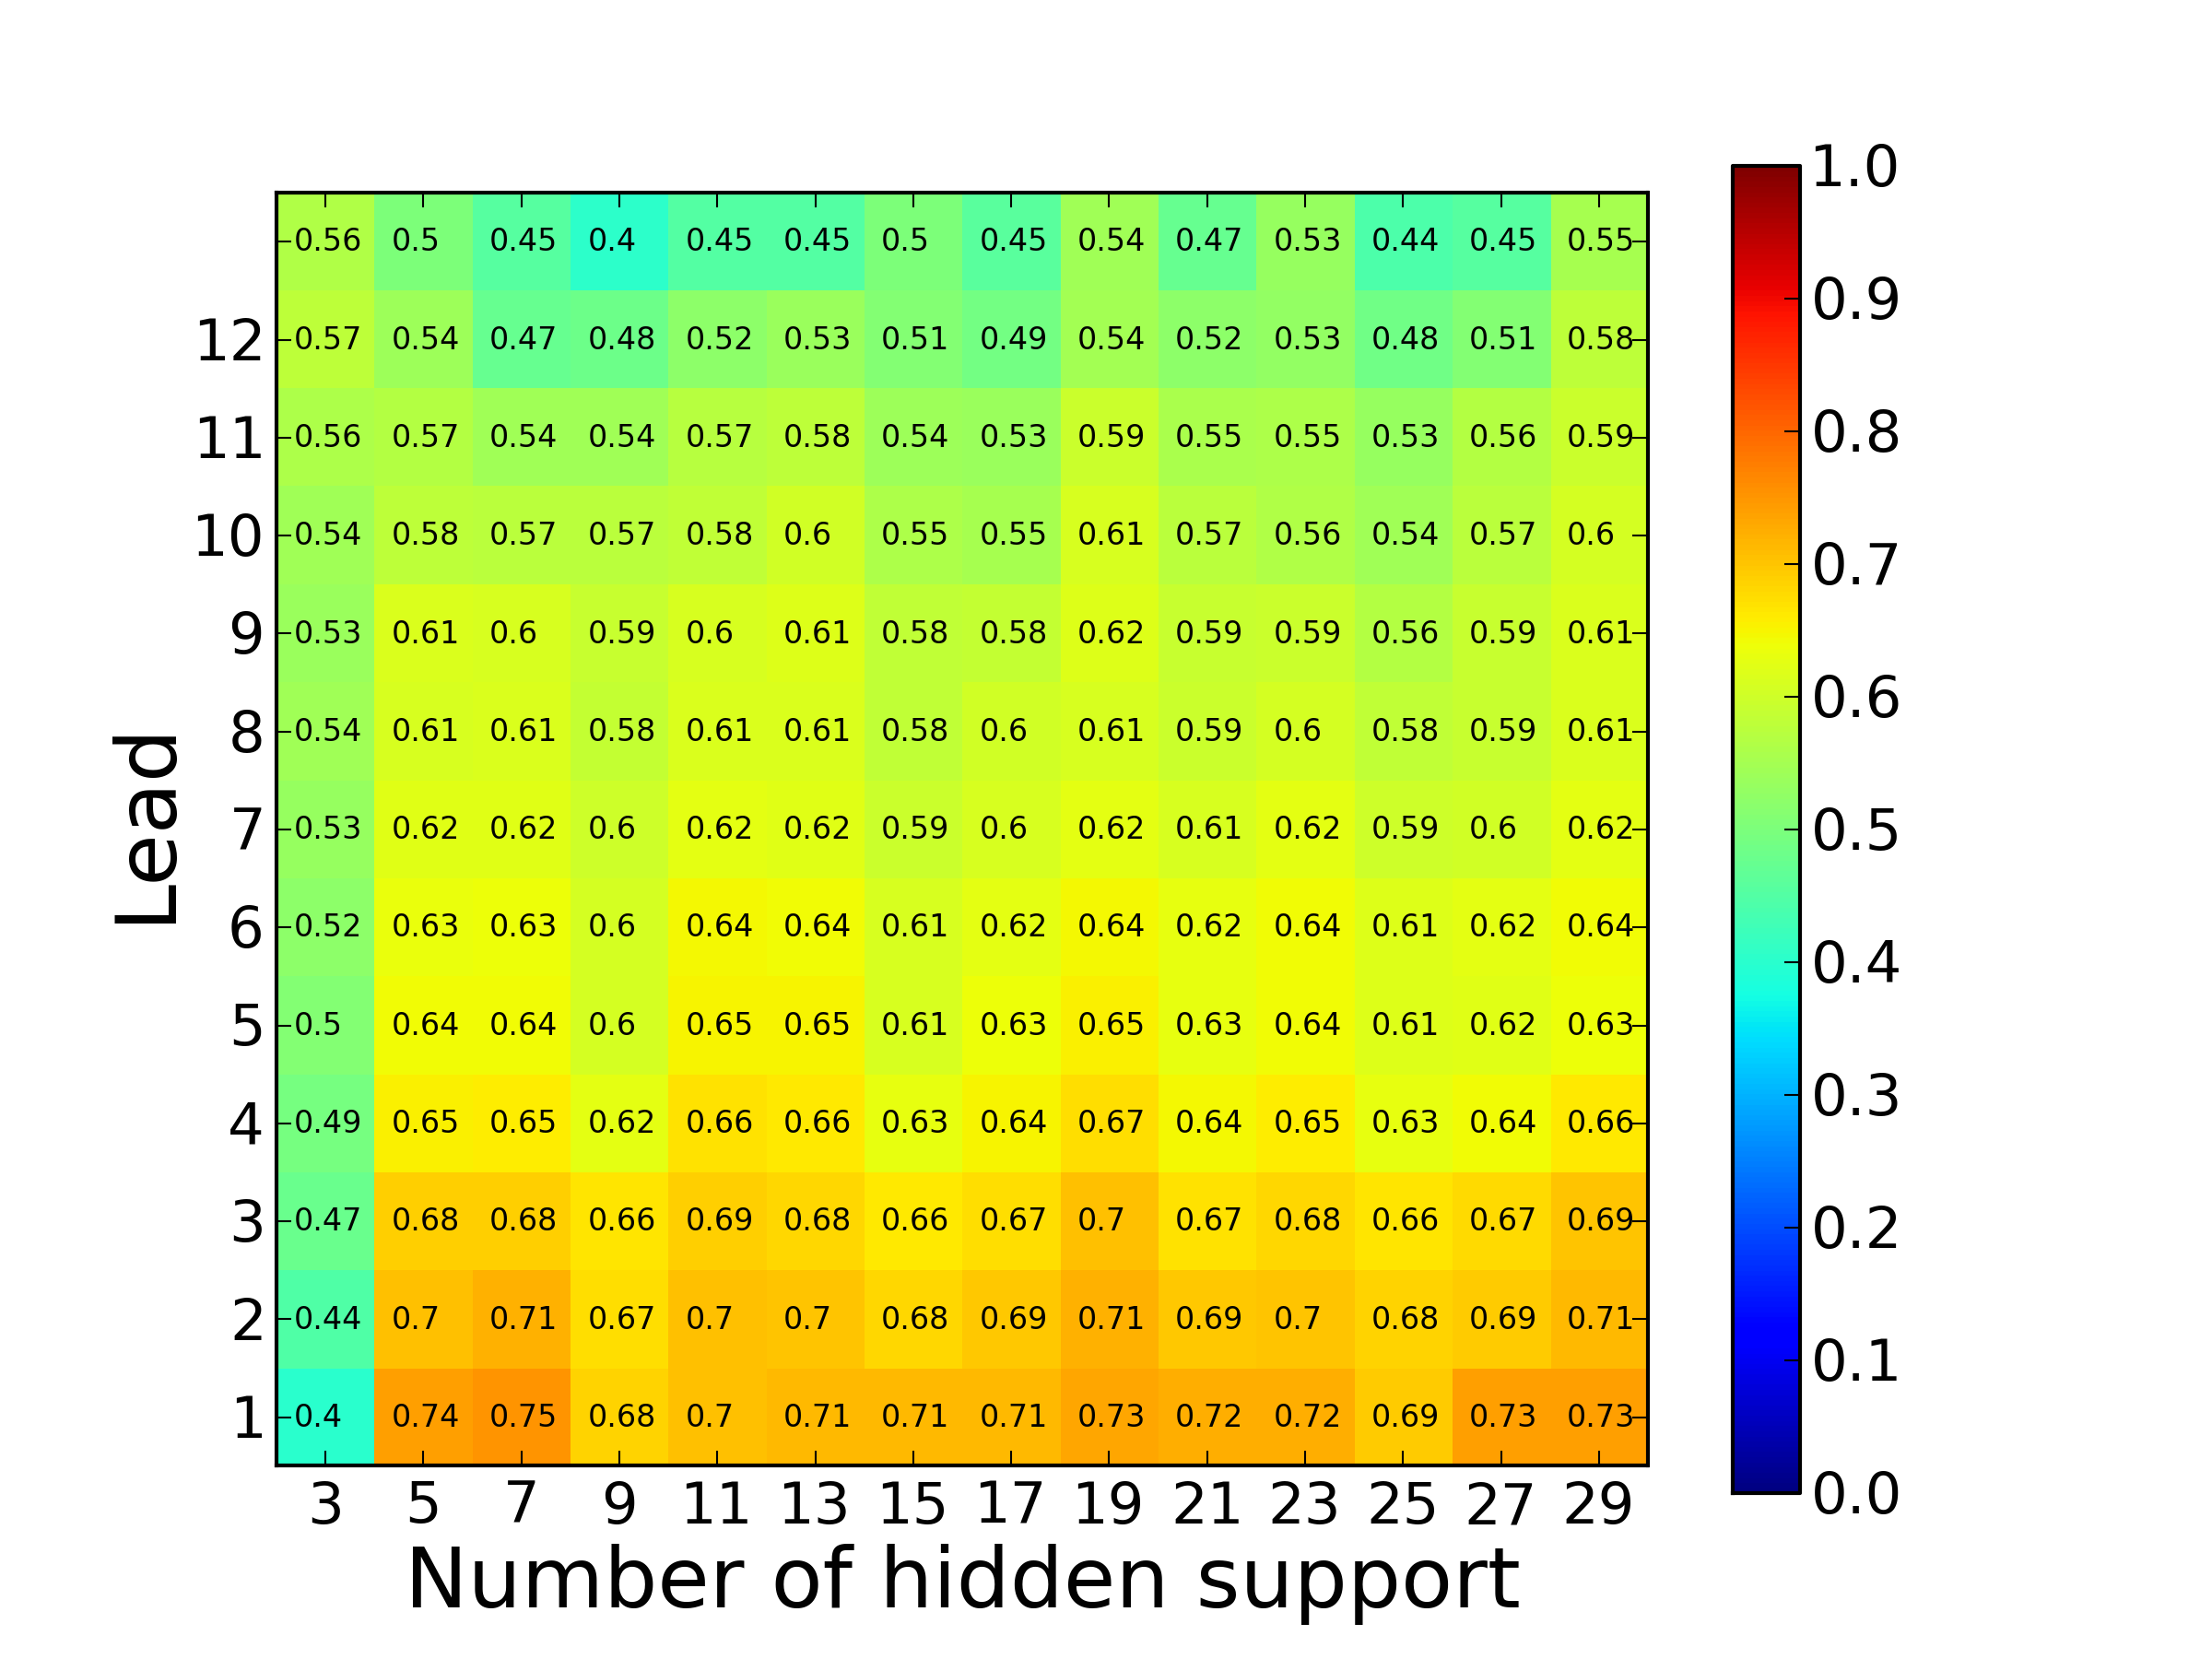
\includegraphics[width=1.0\textwidth]{figures/hmm/forum_and_wiki.png}
\end{figure}

\begin{figure}[ht!]
  \caption{Heatmap for the \wiki cohort.}\label{fig:hmm_heatmap_wiki_only}
  \centering
    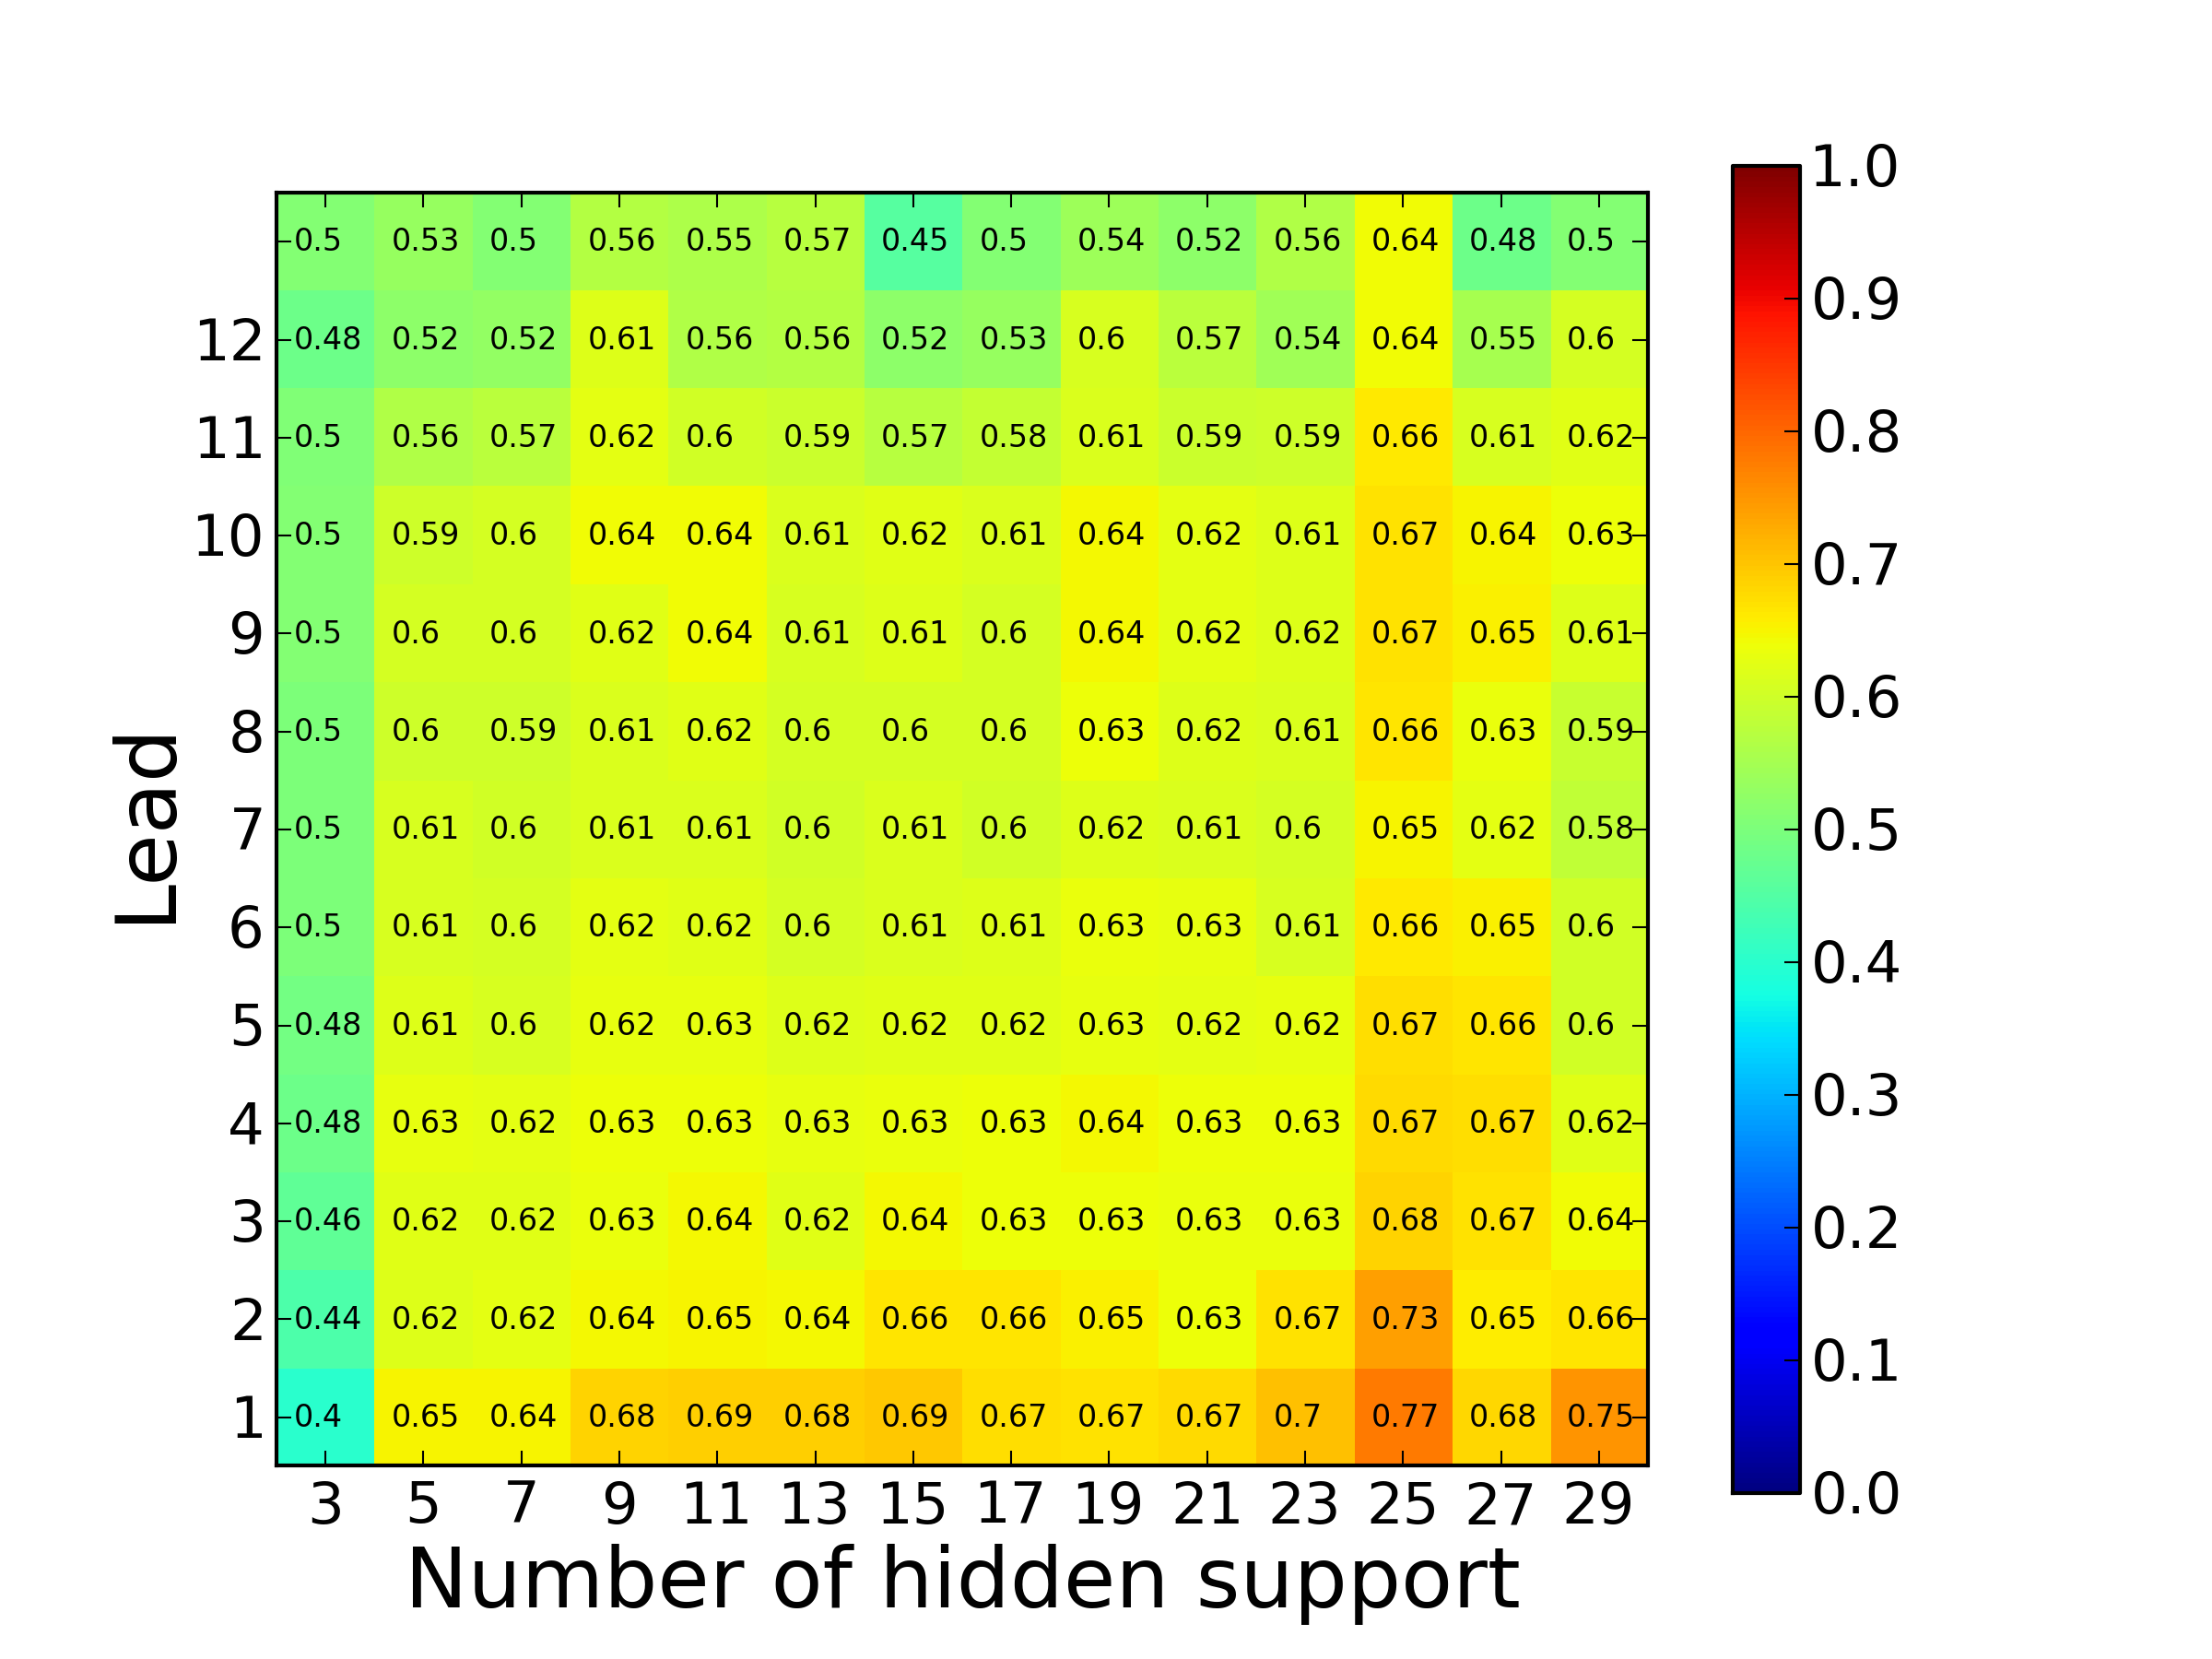
\includegraphics[width=1.0\textwidth]{figures/hmm/wiki_only.png}
\end{figure}

Figures \ref{fig:hmm_heatmap_no_collab} to \ref{fig:hmm_heatmap_wiki_only} show HMM heatmaps for all four cohorts using features that did not undergo principal component analysis. Interestingly, they achieved much different results than the HMMs with PCA. For example, Figure \ref{fig:hmm_heatmap_no_collab} performs consistently better than its PCA counterpart. It converges more quickly- achieving near optimal predictive power at K = 11. It outperforms PCA in nearly every experiment (given K greater than 9), and even attains an AUC of 0.9. This provides further evidence that the PCA HMM did not converge, and it could achieve results as good with a higher K.

However, for other cohorts, such as \forum, the PCA HMM \ref{fig:hmm_heatmap_forum_only} consistently out-predicts the HMM without PCA. The PCA HMM achieves an AUC of ~.78 for all K greater than 19 and lead of one, whereas its non-PCA HMM only hits ~0.82. Similar differences exist in the \both cohort in \ref{fig:hmm_heatmap_forum_and_wiki}. In both of these cohorts, it appears that the PCA HMM used a high enough K to converge to the correct number of modes of students.

One last difference between the non-PCA HMMs and the PCA HMMs is that the non-PCA model's predictive power degrades more gracefully as the lead increases. This remains to be explained and requires more investigation.

\begin{figure}[ht!]
  \caption{Mean AUC as K increases for the \neither cohort.}\label{fig:hmm_support_over_time_no_collab}
  \centering
    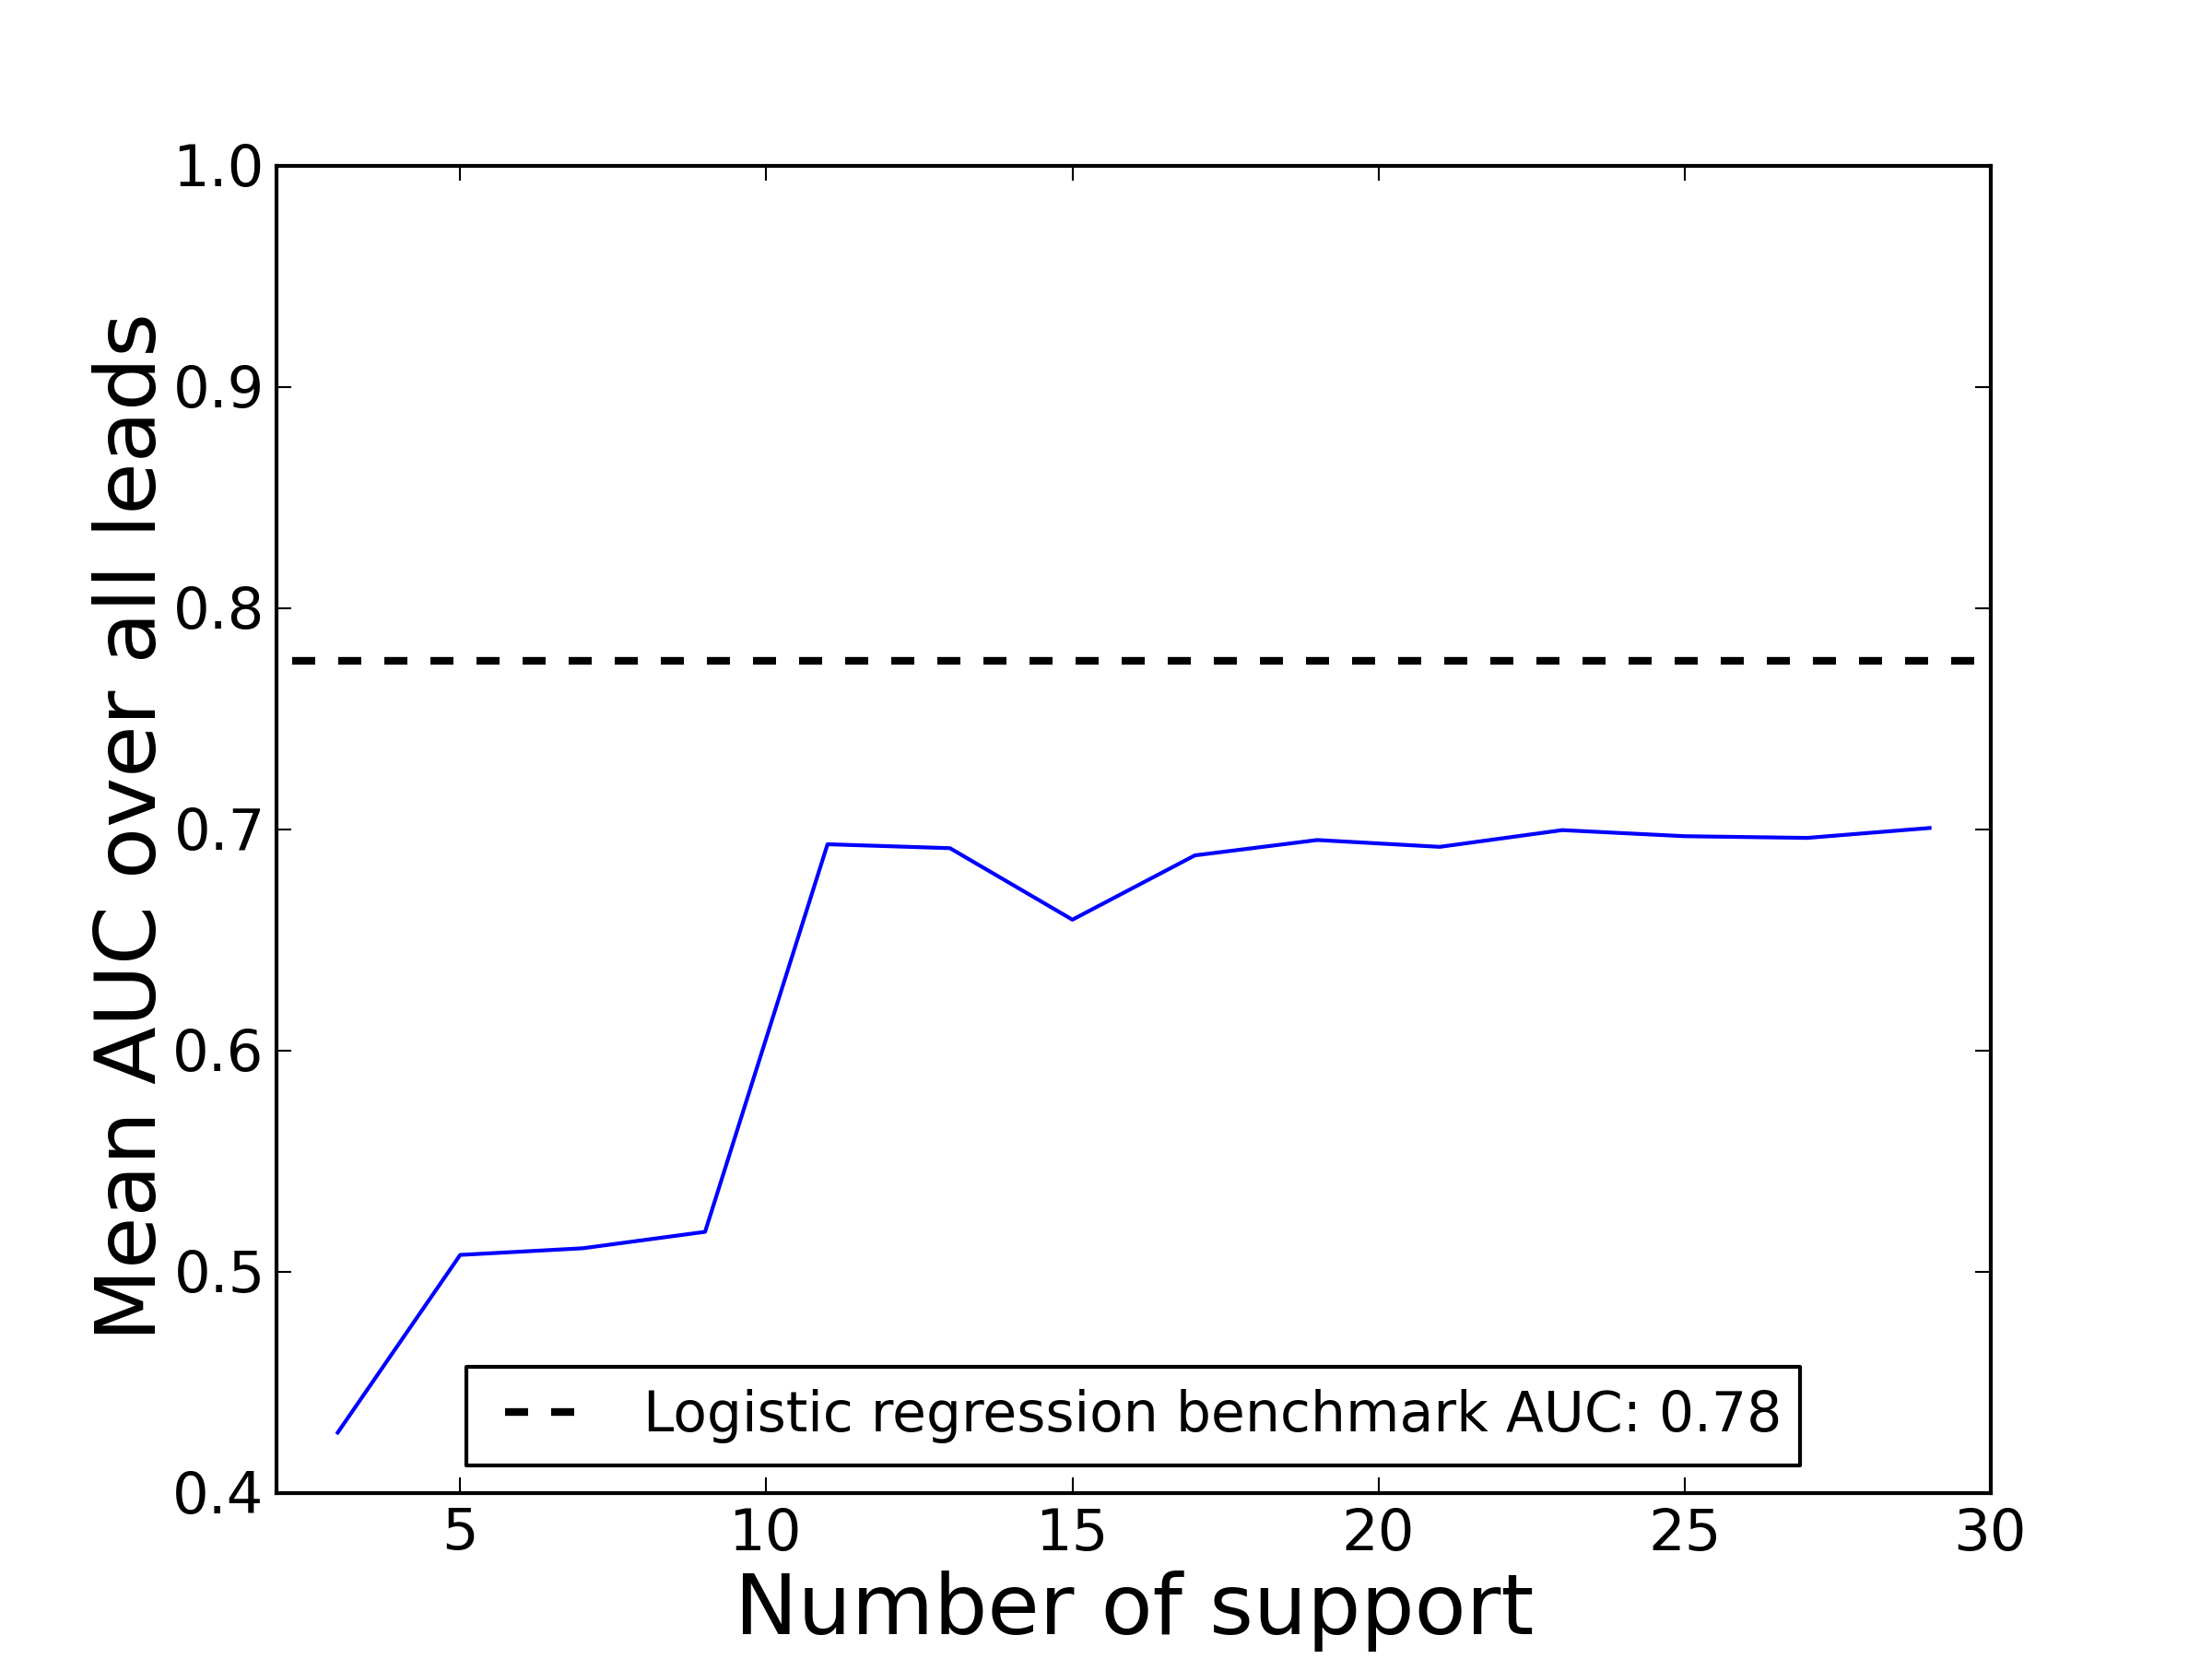
\includegraphics[width=0.8\textwidth]{figures/hmm/no_collab_support_over_time.png}
\end{figure}

\begin{figure}[ht!]
  \caption{Mean AUC as K increases for the \forum cohort.}\label{fig:hmm_support_over_time_forum_only}
  \centering
    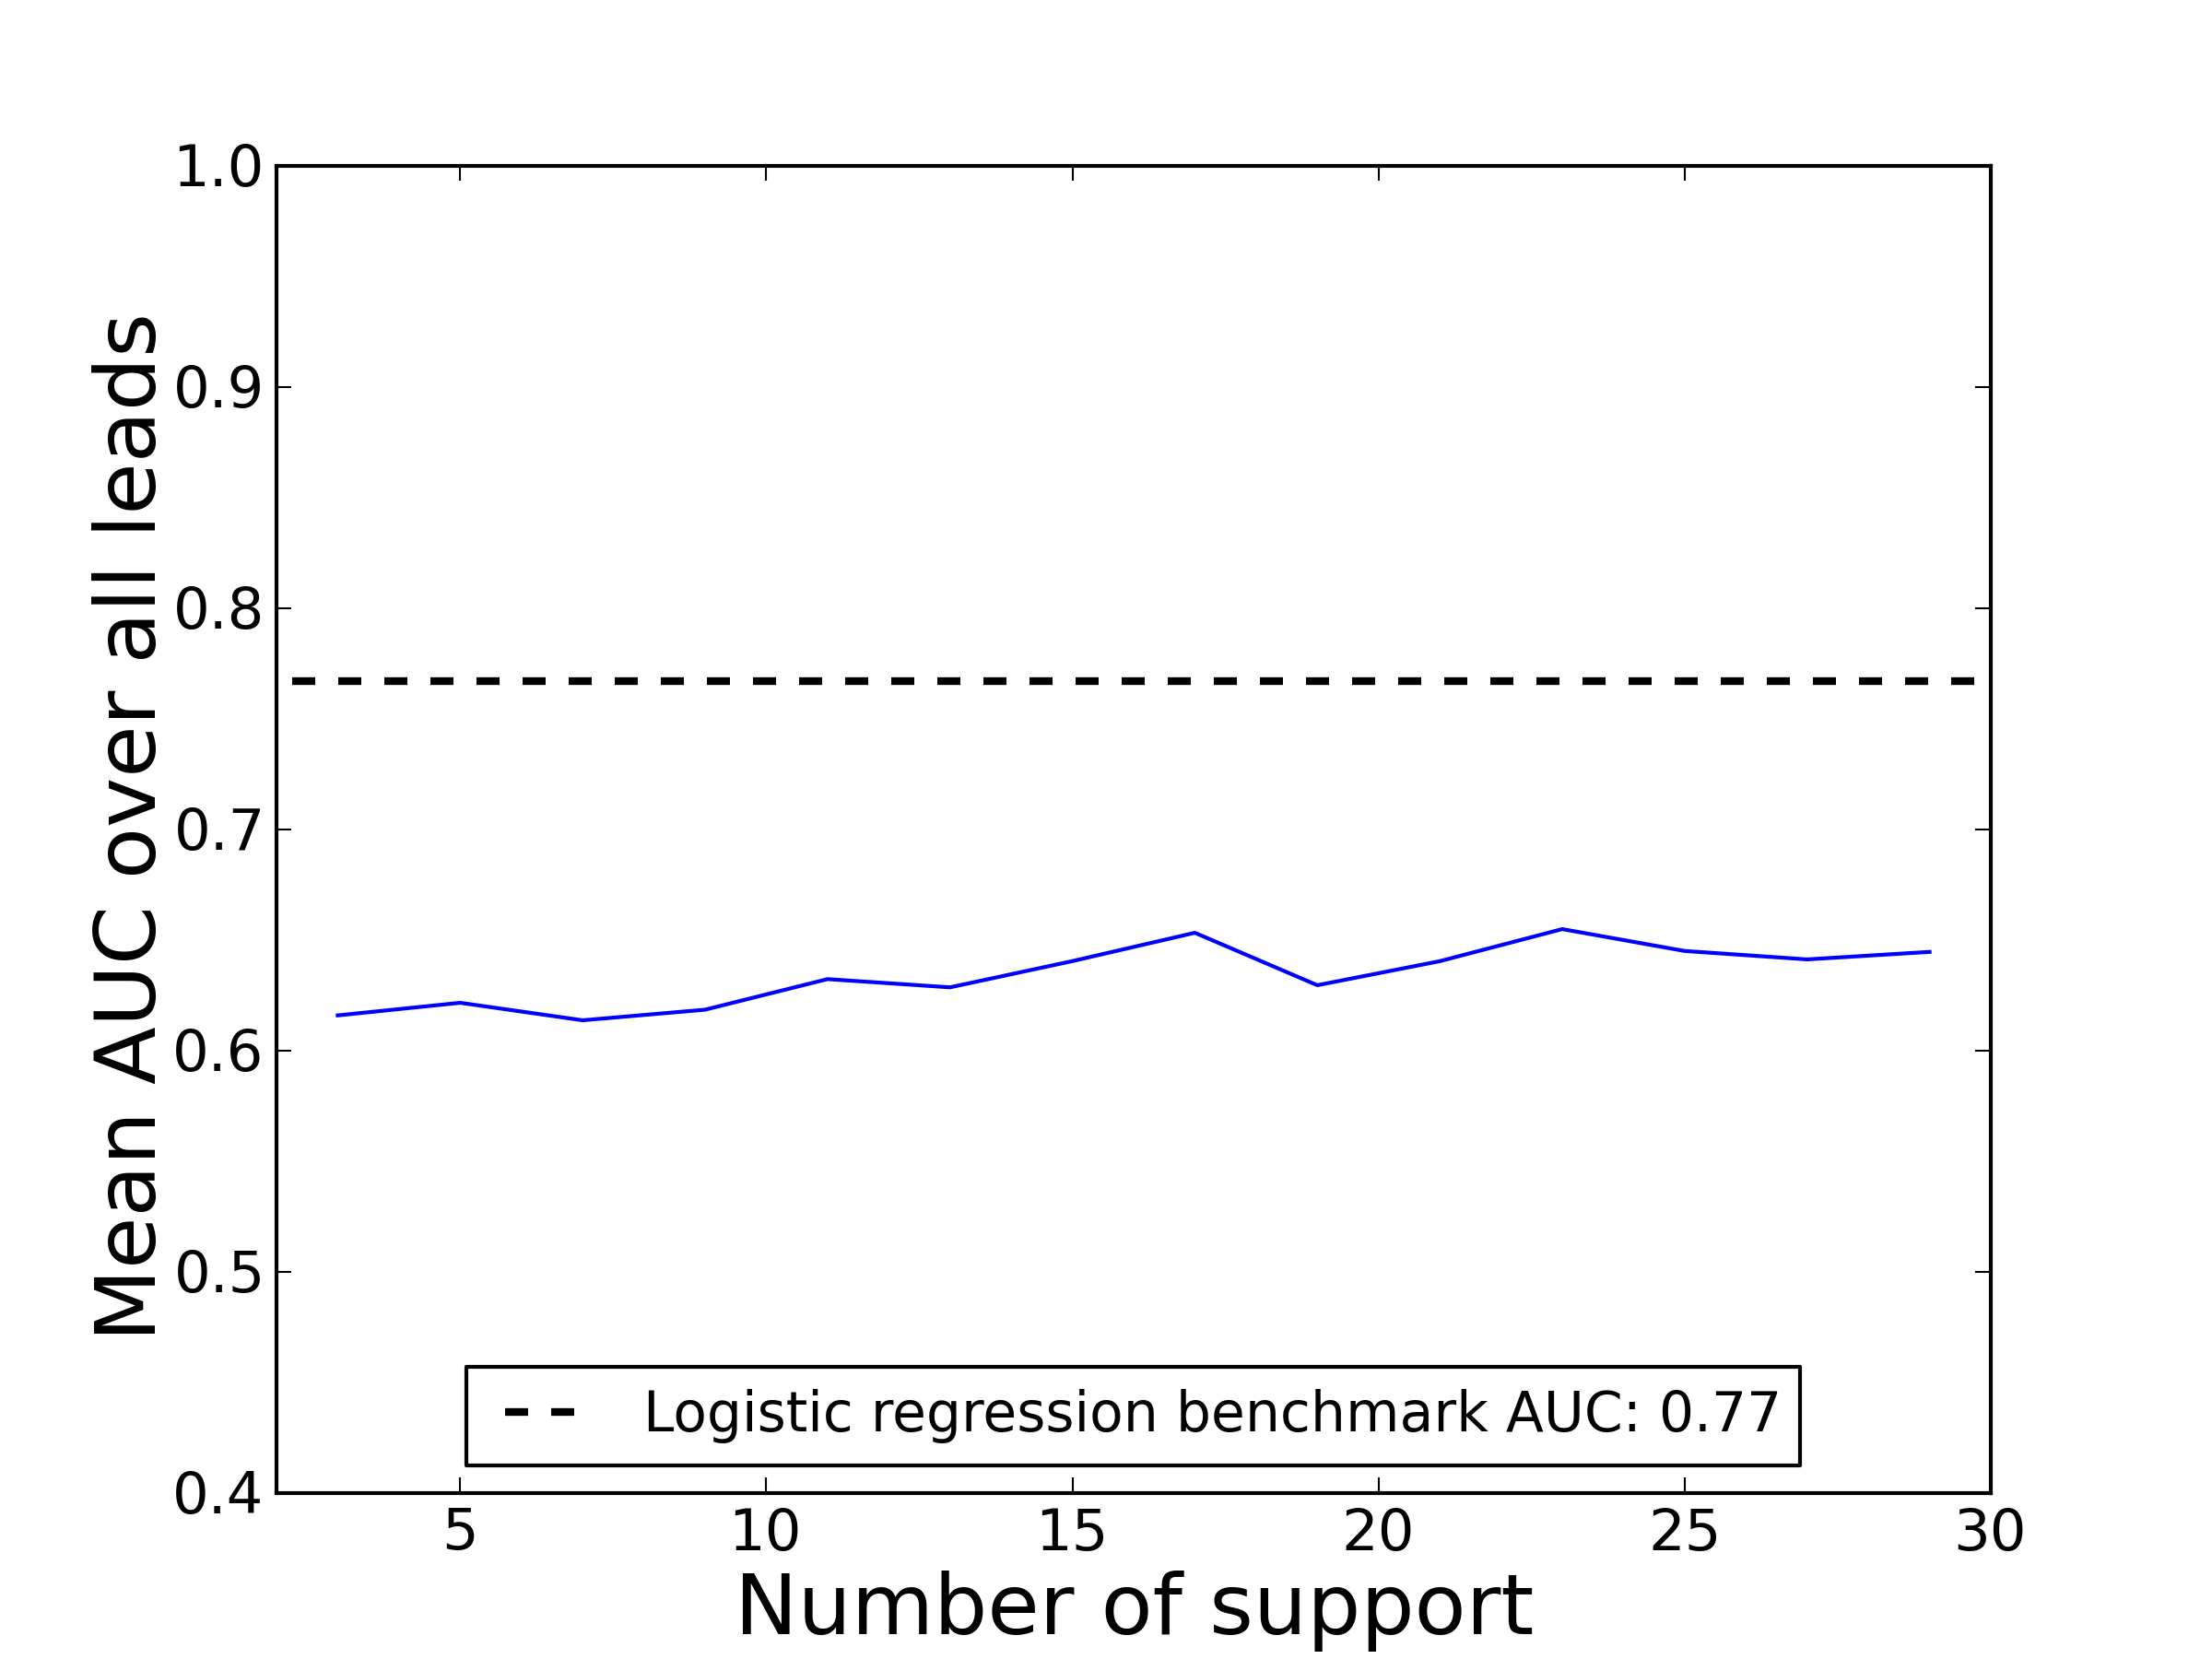
\includegraphics[width=0.8\textwidth]{figures/hmm/forum_only_support_over_time.png}
\end{figure}

\begin{figure}[ht!]
  \caption{Mean AUC as K increases for the \both cohort.}\label{fig:hmm_support_over_time_forum_and_wiki}
  \centering
    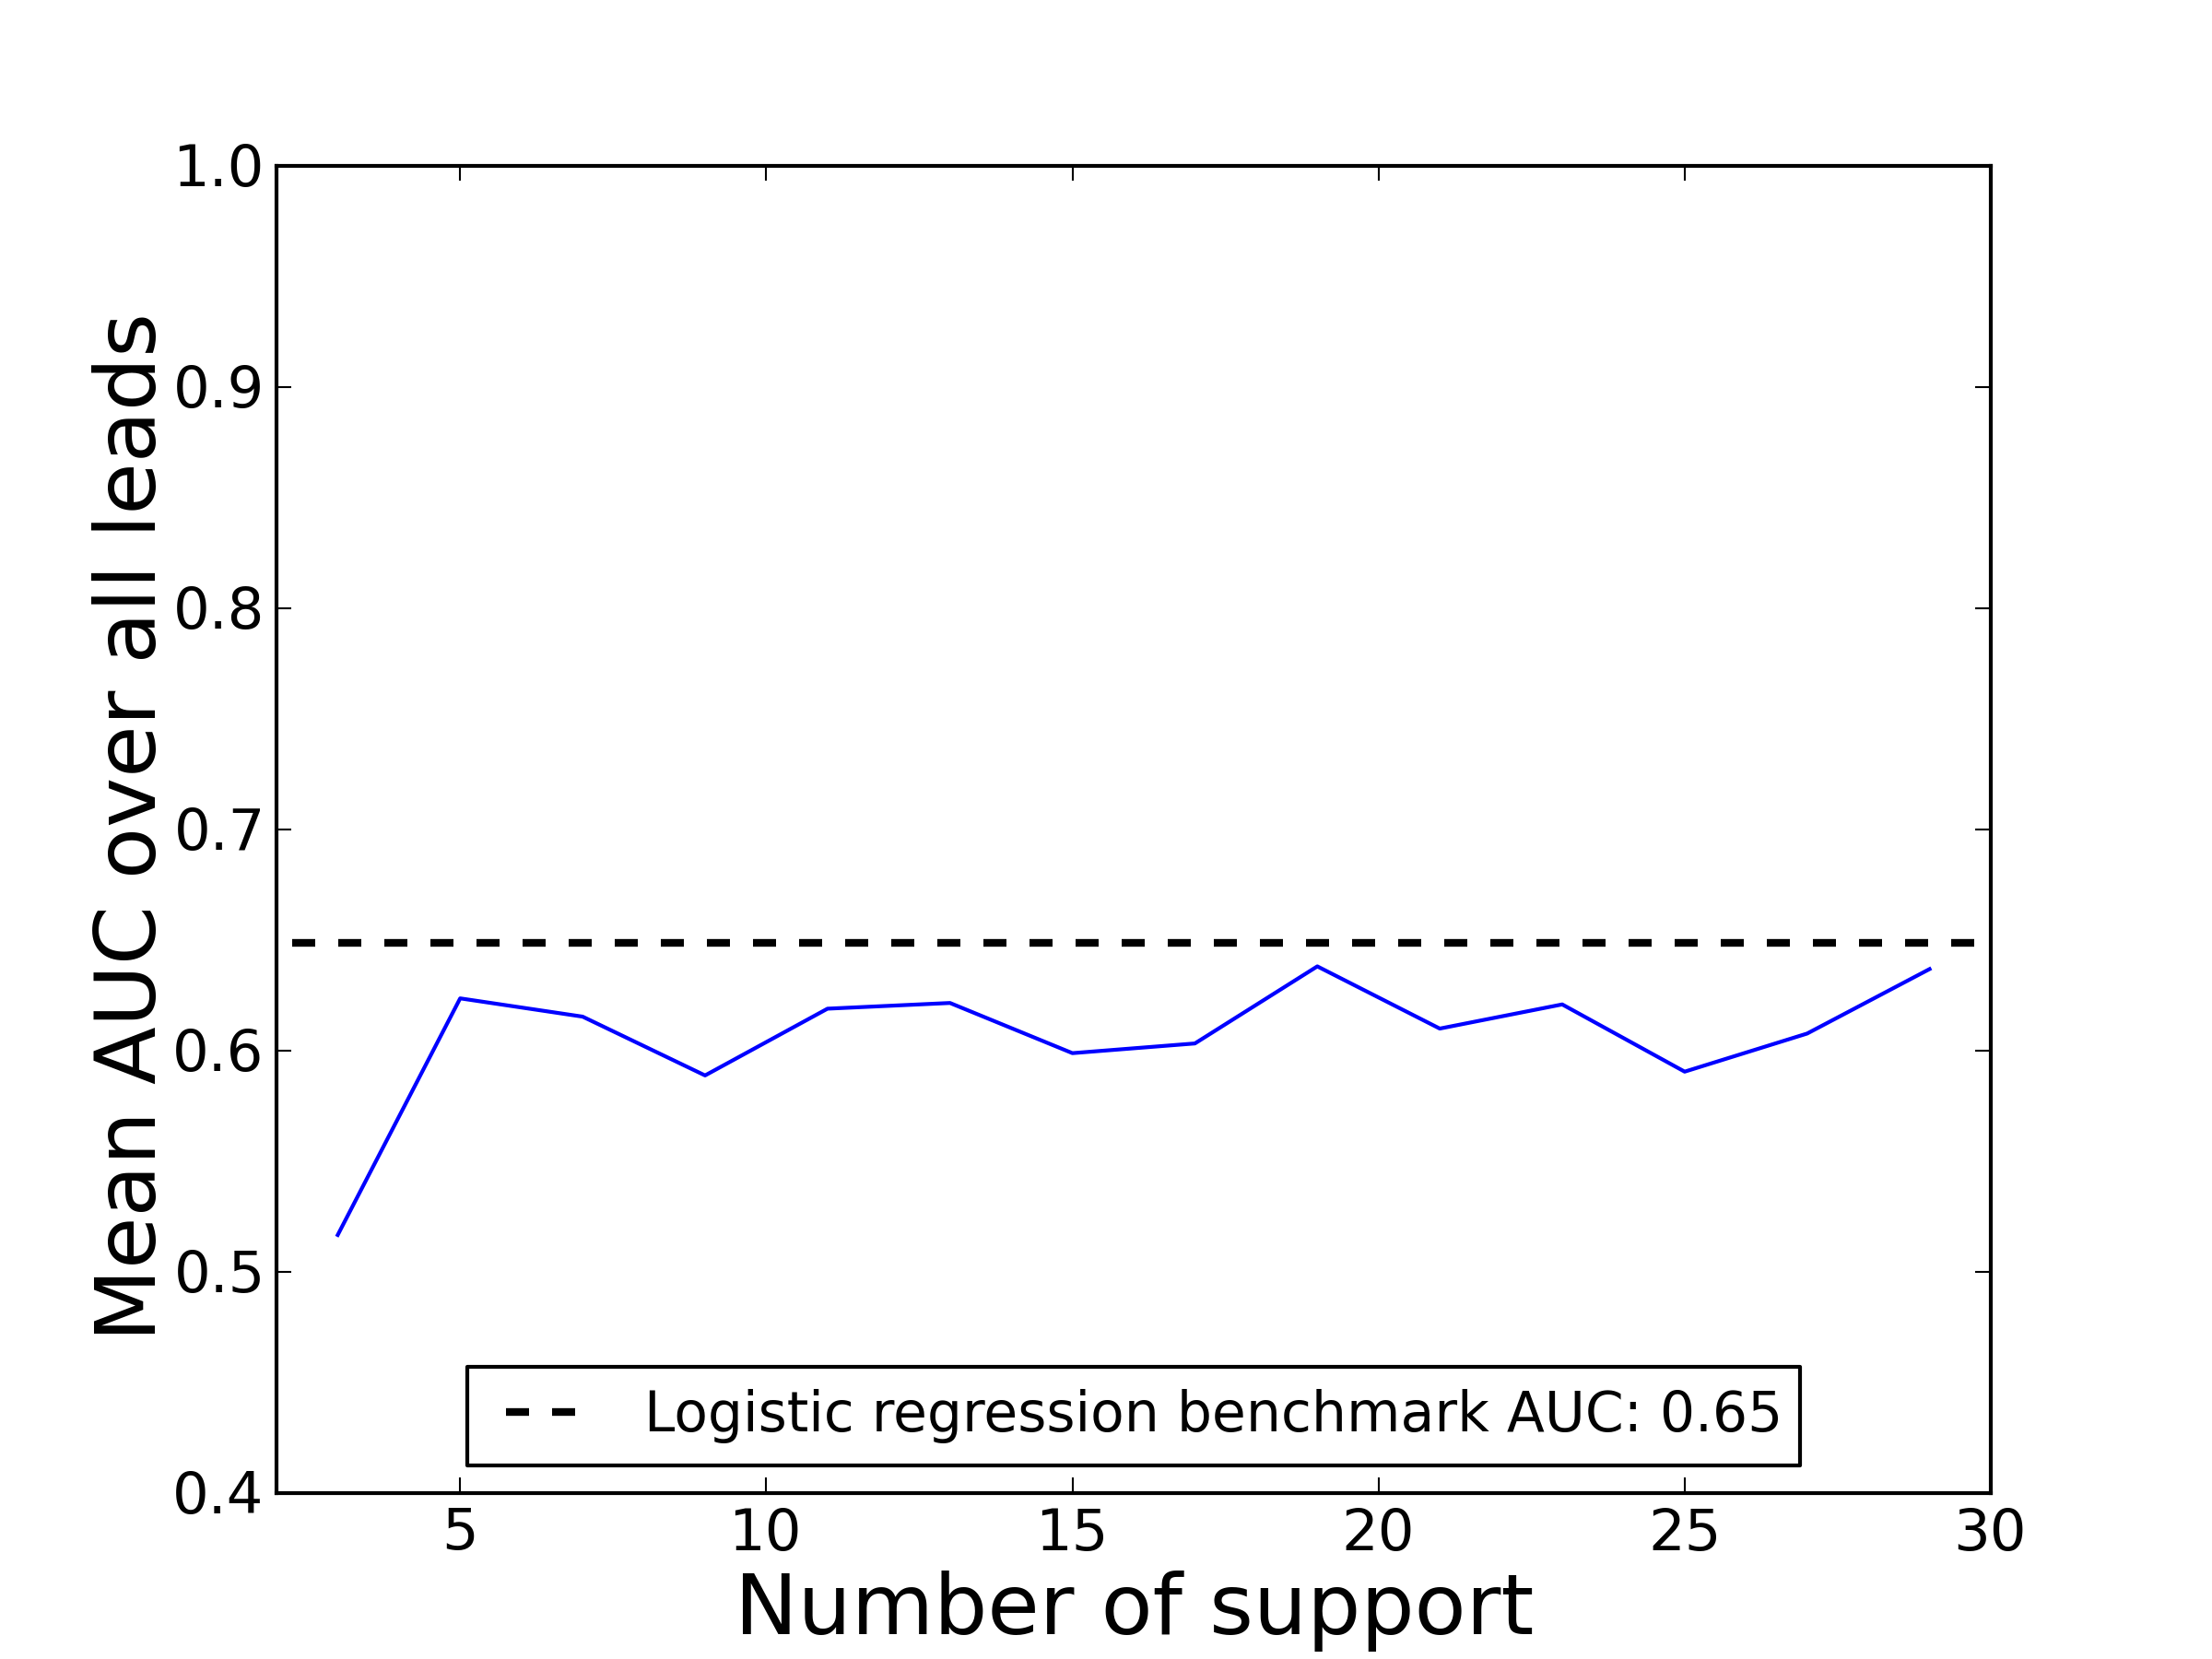
\includegraphics[width=0.8\textwidth]{figures/hmm/forum_and_wiki_support_over_time.png}
\end{figure}

\begin{figure}[ht!]
  \caption{Mean AUC as K increases for the \wiki cohort.}\label{fig:hmm_support_over_time_wiki_only}
  \centering
    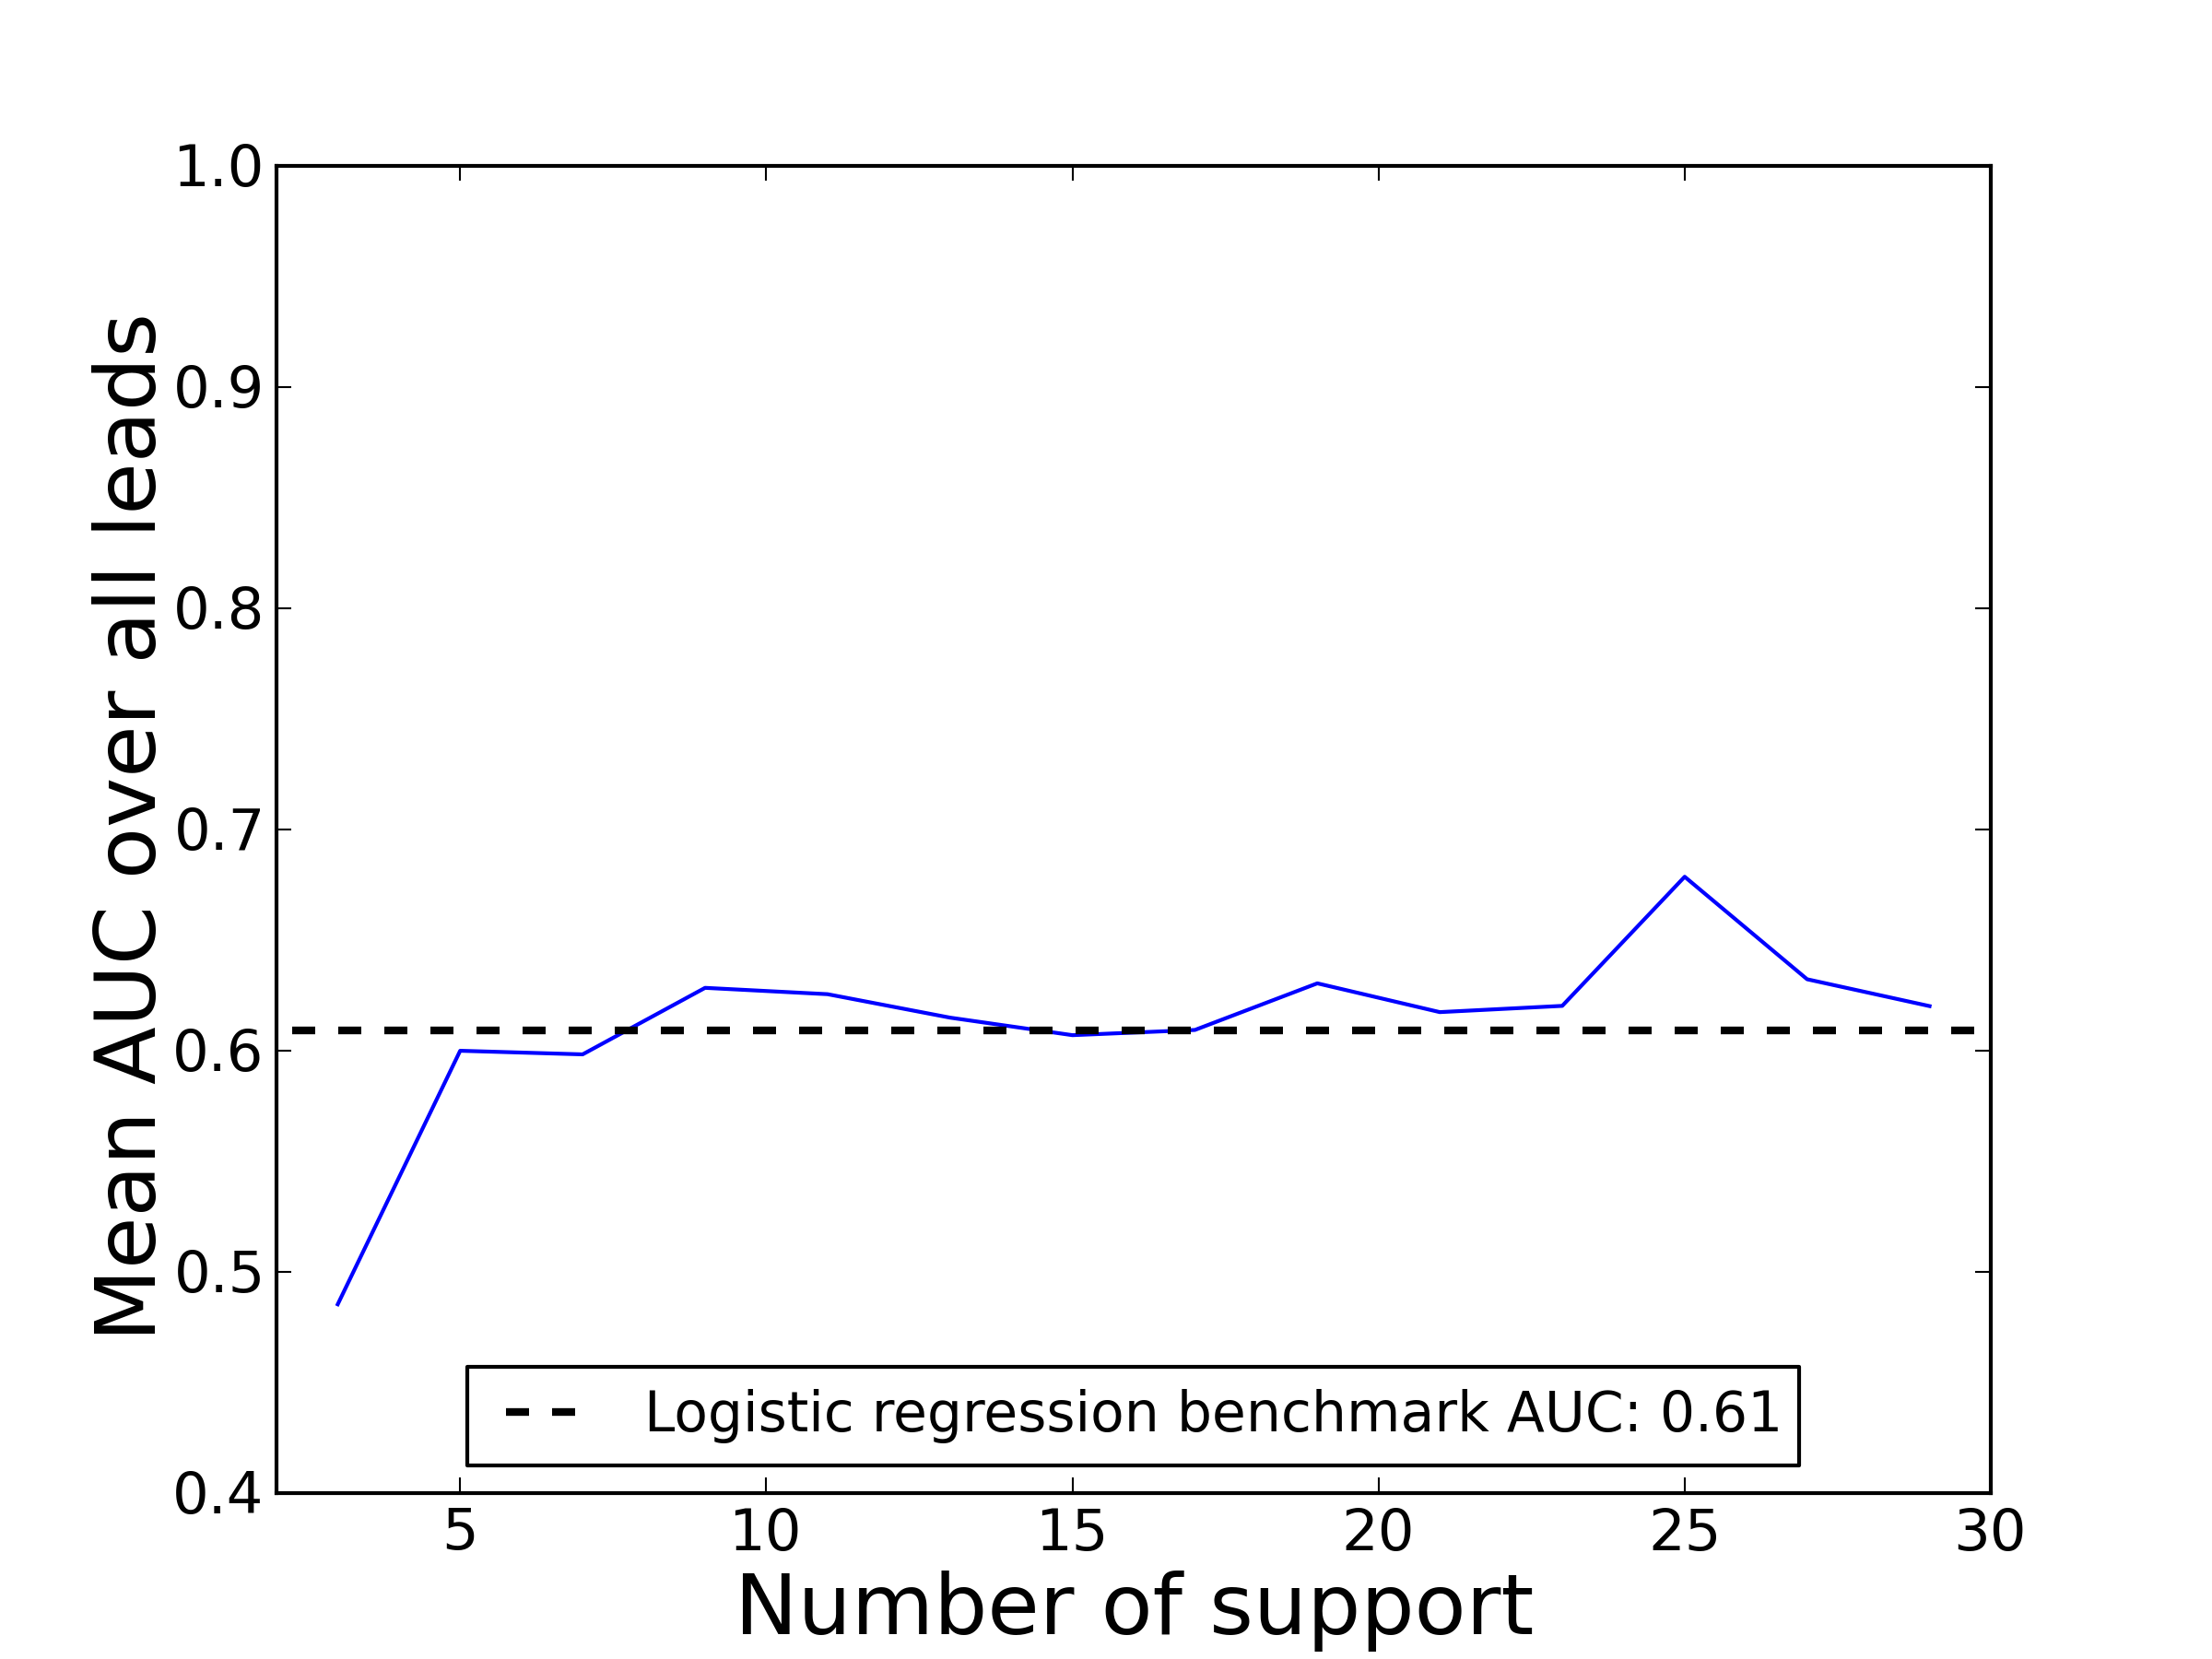
\includegraphics[width=0.8\textwidth]{figures/hmm/wiki_only_support_over_time.png}
\end{figure}

In figures \ref{fig:hmm_support_over_time_no_collab} through \ref{fig:hmm_support_over_time_wiki_only} we look at how the mean AUC changes as K increases for the non-PCA HMMs. We see the AUCs converge much faster than the PCA HMMs. In addition, the mean AUC comes closer to the benchmark logistic regression mean AUC. This is especially true for the smaller \wiki and \both cohorts, on which logistic regression performs poorly due to a lack of data. Indeed, the \wiki HMM outperforms its logistic regression counterpart for almost all values of K.

At this point in the thesis, Chapter \ref{chap:logreg} has described models with logistic regression and Chapter \ref{chap:hmm} with HMMs. HMMs rarely generated AUC results better than logistic regression and were more predictively accurate when we used features not reduced by PCA. Perhaps the best value derived from HMMs is the insight into a hidden state and its support. In Chapter \ref{chap:logreg_hmm} attempt to leverage the hidden state unmasked by HMMs can be used with logistic regression modelling to further extend prediction.







% \begin {center}
% \begin {tikzpicture}[-latex ,auto ,node distance =4 cm and 5cm ,on grid ,
% semithick ,
% state/.style ={ circle ,top color =white , bottom color = processblue!20 ,
% draw,processblue , text=blue , minimum width =1 cm}]
% \node[state] (C)
% {$1$};
% \node[state] (A) [above left=of C] {$0$};
% \node[state] (B) [above right =of C] {$2$};
% \path (A) edge [loop left] node[left] {$1/4$} (A);
% \path (C) edge [bend left =25] node[below =0.15 cm] {$1/2$} (A);
% \path (A) edge [bend right = -15] node[below =0.15 cm] {$1/2$} (C);
% \path (A) edge [bend left =25] node[above] {$1/4$} (B);
% \path (B) edge [bend left =15] node[below =0.15 cm] {$1/2$} (A);
% \path (C) edge [bend left =15] node[below =0.15 cm] {$1/2$} (B);
% \path (B) edge [bend right = -25] node[below =0.15 cm] {$1/2$} (C);
% \end{tikzpicture}
% \end{center}
\chapter{Logistic Regression of the HMM Hidden State Distribution} \label{chap:logreg_hmm} 

\section{Background}
A powerful way to use predictive models is to combine them. One possible way to do so is to use a hidden markov model to infer the hidden state of an entity each time slice, and then use the probability distribution outcomes of the hidden state as features for another predictive model. Applying HMM inference gives the probabilities at being in each hidden state for a given time-slice. These probabilities are used as features for the next classifier. In this example, we use the hidden state probability distribution as features for a time-slice, and apply logistic regression with the resulting feature-vector. We call this model logistic regression on HMM state.

For example, let's say that we want to apply logistic regression on the HMM hidden state distribution for a hidden state support of 3, lag of 3 and lead of 5. To perform inference on the HMM model, we would pass 3 weeks of data to the model, and ask for the hidden state probability distribution for each of three weeks. Each week would have a 3 element distribution (because there are 3 hidden states). Figure \ref{fig:hmm_as_logreg} shows a diagram of how the logistic regression feature vector is created. Only two of these are relevant (because the 3 numbers always add to 1). Next, we would take the first two probabilities from each of the 3 week's distributions, and use these 6 probabilities as a feature vector in logistic regression. The label of the data point is the stopout value for week 8.

\begin{figure}[!ht]
  \caption{Diagram showing how the logistic regression feature vector is created using the HMM hidden state probabilities as features.}\label{fig:hmm_as_logreg}
  \centering
    \includegraphics[width=0.8\textwidth]{figures/hmm_as_logreg}
\end{figure}

The intuition for why this might be a valid approach is that, in a way, the hidden state is a less noisy description of the observed variables. For example, in the stopout problem, the hidden state could represent the type of student, and the features are simply noisy observations. Constructing an HMM thus creates a less noisy description of the data. 

\section{Predicting stopout using logistic regression on HMM state}
We used the same parameters and software as in the individual models. This included a range of supports from 3 to 29, with a step size of 2, a maximum number of Baum-Welch iterations of 100, and a log-likelihood differential threshold of 0.0000001.

\subsection{Experimental setup}
The process to construct such a model is more complex than the previous two models. It entails the following, for each lead, lag and hidden support combination:
\begin{enumerate}
\item Split the train dataset into two equal partitions. I call the first `construct hmm' and the second `generate features'. We partition the data in order to not pollute the inference of the HMM with data it has been trained on.
\item Train an HMM on the `construct hmm' partition. Similarly to the normal HMM case, we trained 10 models to compensate for the potential to get stuck on a local maximum. We selected the best model to use based on the likelihood score of the Baum-Welch algorithm. We also performed this in parallel, as training can take significant amounts of time. We train this HMM once for each support, but use the same model for each lead and lag combination
\item Perform inference on the `generate features' partition. We asked the model to generate the hidden state probability distribution for each week in lag weeks, and took K -1 of these probabilities for each lag week as features for the model (where K is the hidden support). These feature vectors and labels become the training dataset for logistic regression.
\item Perform 10 fold cross validation, using the generated training dataset. 
\item Train a logistic regression model on the generated training dataset.
\item Perform inference on the actual test dataset by putting each data point through the model and comparing the resulting probability of stopout versus the truth stopout label.
\item Evaluate the model using mean cross-validation ROC AUC and test set ROC AUC.
\end{enumerate}

\section{Logistic regression on HMM state results}
Figures \ref{fig:hmm_logreg_heatmap_no_collab} through \ref{fig:hmm_logreg_heatmap_wiki_only} summarize the AUC of the receiver operating characteristic for all four cohorts over each lead and \lag combinations, similar to those in Chapter \ref{chap:logreg}. In order to compare, we choose the K with the best mean AUC for all 91 experiments. The chosen mean is indicated.

\begin{figure}[ht!]
  \caption{Heatmap of the \neither cohort. PCA transformations of features used. The shown heatmap used a support of 27 for the HMM. This was the support which yielded the highest mean AUC.}\label{fig:hmm_logreg_heatmap_no_collab}
  \centering
    \includegraphics[width=1.0\textwidth]{figures/hmm_logreg/no_collab_pca_support_27.png}
\end{figure}

\begin{figure}[ht!]
  \caption{Heatmap of the \forum cohort. PCA transformations of features used. The shown heatmap used a support of 21 for the HMM. This was the support which yielded the highest mean AUC.}\label{fig:hmm_logreg_heatmap_forum_only}
  \centering
    \includegraphics[width=1.0\textwidth]{figures/hmm_logreg/forum_only_pca_support_21.png}
\end{figure}

\begin{figure}[ht!]
  \caption{Heatmap of the \both cohort. PCA transformations of features used. The shown heatmap used a support of 19 for the HMM. This was the support which yielded the highest mean AUC.}\label{fig:hmm_logreg_heatmap_forum_and_wiki}
  \centering
    \includegraphics[width=1.0\textwidth]{figures/hmm_logreg/forum_and_wiki_pca_support_19.png}
\end{figure}

\begin{figure}[ht!]
  \caption{Heatmap of the \wiki cohort. The shown heatmap used a support of 7 for the HMM. This was the support which yielded the highest mean AUC.}\label{fig:hmm_logreg_heatmap_wiki_only}
  \centering
    \includegraphics[width=1.0\textwidth]{figures/hmm_logreg/wiki_only_support_7.png}
\end{figure}

The HMM logistic regression models perform similarly to the logistic regression models. Their AUCs are more polarized, however, due to the constant transition matrix, as described in chapter \ref{chap:hmm}. For short leads, HMM logistic regression out-predicts logistic regression, but its performance decreases faster as the lead increases. 

\begin{figure}[ht!]
  \caption{Mean AUC as K increases for the \neither cohort. PCA transformations of features used.}\label{fig:hmm_logreg_support_over_time_no_collab_pca}
  \centering
    \includegraphics[width=0.8\textwidth]{figures/hmm_logreg/no_collab_pca_support_over_time.png}
\end{figure}

\begin{figure}[ht!]
  \caption{Mean AUC as K increases for the \forum cohort. PCA transformations of features used.}\label{fig:hmm_logreg_support_over_time_forum_only_pca}
  \centering
    \includegraphics[width=0.8\textwidth]{figures/hmm_logreg/forum_only_pca_support_over_time.png}
\end{figure}

\begin{figure}[ht!]
  \caption{Mean AUC as K increases for the \both cohort. PCA transformations of features used.}\label{fig:hmm_logreg_support_over_time_forum_and_wiki_pca}
  \centering
    \includegraphics[width=0.8\textwidth]{figures/hmm_logreg/forum_and_wiki_pca_support_over_time.png}
\end{figure}

\begin{figure}[ht!]
  \caption{Mean AUC as K increases for the \wiki cohort.}\label{fig:hmm_logreg_support_over_time_wiki_only}
  \centering
    \includegraphics[width=0.8\textwidth]{figures/hmm_logreg/wiki_only_support_over_time.png}
\end{figure}

Figures \ref{fig:hmm_logreg_support_over_time_no_collab_pca} through \ref{fig:hmm_logreg_support_over_time_wiki_only} show how overall predictive accuracies of the HMM models change as K increases. The logistic regression mean AUC is also shown as a benchmark. The only cohort which outperforms logistic regression is \both, presumably because HMM model is able to train with less students. All cohorts except for \wiki converge around K of 21.
\chapter{Discriminative Classifiers: Delphi} \label{chap:delphi} 
\section{Background}
Delphi is a first-ever shared machine learning service. It is a multi-algorithm, multi-parameter self-optimizing machine learning system that attempts to automatically find and generate the optimal discriminative model. A hybrid Bayesian and Multi-armed Bandit optimization system works in a load balanced fashion to quickly deliver results in the form of ready-to-predict models, confusion matrices, cross validation accuracy, training timings, and average prediction times. Delphi works by creating a very high dimensional search space of models and parameters. It navigates this space by trying many different combinations, and gravitating towards models with better results (in terms of prediction accuracy). It was built by an M.Eng. student in the ALFA group. Delphi uses a wide array of classification algorithms, most of which are implementations from scikit-learn. The explanations for each are outside the scope of this thesis.

\section{Predicting stopout using Delphi}

\subsection{Experimental setup}
In order to run our datasets through Delphi, we performed the following:
\begin{enumerate}
\item Chose a few lead, lag combinations to run on Delphi. Since Delphi creates many models, we only chose 3 datasets per cohort. We chose lead and lag combinations which were difficult for logistic regression to predict so we could see if Delphi would perform better. We chose the following combinations: lead of 13, lag of 1; lead of 3, lag of 6; lead of 6, lag of 4.
\item Flattened each cohort's train and test dataset to generate files which could be passed to Delphi. We flattened in the same manner as described in logistic regression section.
\item Ran the 12 datasets through Delphi. This gave us 12 models which performed best on a mean cross validation prediction accuracy metric.
\item Evaluated these models on the basis of test dataset ROC AUC and cross validation ROC AUC performance.
\end{enumerate}

\section{Delphi results}

The models created by Delphi attained AUCs very similar to those of our logistic regression and HMM models. The best algorithm chosen by Delphi varied depending on which lead, lag and cohort combination was chosen. The algorithms included stochastic gradient descent, k nearest neighbors, logistic regression, support vector machines and random forests.

For the two larger cohorts, \neither and \forum, Delphi's models used logistic regression, stochastic gradient descent, support vector machines and random forests. For each of the lead and lag combinations, the models' results were with 0.02 of our logistic regression results. This indicated that the predictive power of these cohorts was not due to the type of model used. Rather, the strong predictive accuracies achieved were caused by the interpretive features in the models. As previously noted in Chapter \ref{chap:logreg}, varying the features used, such as when using only the \selfself features rather than the \selfself features and \crowdself features, significantly changed the results. These findings led us to conclude that focusing on better features provides more leverage in MOOC data science than does fine-tuning models.

For the smaller \wiki and \both cohorts, Delphi's models provided significantly better accuracy. For example, for the \wiki cohort, all three lead and lag combinations' models produces AUCs greater than 0.85! This indicated that for these cohorts, the type of model matters a great deal. We conclude that this is due to the small size of the cohorts, as some classifiers are able to more gracefully handle less data. The best classifiers used to model these cohorts included k nearest neighbors and stochastic gradient descent.

In Chapters \ref{chap:logreg} through Chapters \ref{chap:delphi} we have presented the models we used in stopout prediction. In the next chapter, we present the framework used to accomplish building these models at scale.
\chapter{Distributed Computing}\label{chap:dcap} 
As described in the previous chapter, we planned on creating a large number of predictive models. In order to scale such a large number of experiments, we needed a parallelization framework to accomplish machine learning at scale, utilizing the computing power of CSAIL's openstack cloud.

In order to accomplish this, we modified a parallelization framework called DCAP to run our experiments. DCAP is a master-slave architected system built in the ALFA group that allows a user to manage the execution list of computational jobs \cite{alex}. The list of jobs is called a taskfile. DCAP takes a taskfile and launches a server to which clients can connect. Each time a client connects, the DCAP server sends it a job (including a config file) from the taskfile. The client executes the job and sends the result back to the master. This repeats until there are no more jobs to accomplish. Figure \ref{fig:dcap} shows the flow of jobs.

\begin{figure}[ht!]
  \caption{The client-server architecture of DCAP. It is used to parallelize the model prediction process.}\label{fig:dcap}
  \centering
    \includegraphics[width=1.0\textwidth]{figures/dcap.png}
\end{figure}

We used DCAP to run a large suite of jobs on the cloud. This involved generating taskfiles and config files for each experiment. In addition, we created scripts to launch clients that will automatically connect to a server. We employed the eucalyptus API to manage cloud nodes. Additionally, we created image snapshots containing the datasets and the model creation code to run. The scripts instructed openstack to launch nodes using the images containing the necessary libraries and datasets. Next, the clients would automatically connect to the server and run jobs until all the tasks were finished.

In particular, we used DCAP to run all HMM and logistic regression on HMM state jobs. These model variants are by far the most computational intensive. This included several job launches as we progressively fine tuned our models. Each run included additional modifications, such as training 10 HMMs per experiment to avoid local maxima, and using feature-sets with dimensionality reduction through principal component analysis. Usually, the runs include 84 jobs. This included both types of models, all 4 cohorts, and 14 different hidden variable supports. Due to computational complexity of the algorithms, the final run included 84 jobs, used 22 12-core machines and took around 1 week to finish. Running experiments at this scale would not have been possible if it were not for cloud computing. Using DCAP to do so saved a lot of micro-managing, as everything was ran through scripts automatically.
\chapter{Conclusion}\label{chap:conc}
\section{Data science discussion}
For a successful data science endeavor, there are many critical components. As presented in this thesis, there are numerous challenges in assembling features and a number of data representations one could try and a number of ways to model.  One has to be thorough and systematic, otherwise one will never know if one has got the best prediction capability (thorough in feature definition, model exploration).

\paragraph{Feature engineering}
One has to be meticulous \textbf{from the data up} -- any vague assumptions, quick and dirty data conditioning or preparation will create weak foundations for your modeling and analyses. Many times painstaking manual labor is required - such as manually matching up pset deadlines, etc. You need to be ready to think creatively as you brainstorm and extract features, and be flexible in the ways you assemble them. For example, utilizing the crowd is much richer than just your own expertise.

\paragraph{Machine learning/modeling at scale} 
There are many ways to represent the extracted features data- with or without PCA, temporal and non-temporal, discretized and non discretized. Additionally there are a number of modeling choices - discriminative, generative or mixed models which include many types of classifiers. One has to consider a number of them to enable insights at scale. The alternative results in a much smaller scope with more limited results.

Our ability to build 10,000 models relied on us first building the cloud scale platforms. This is especially true as the machine learning process includes iterations over data definitions, features and cohort definitions. Only through a large scale computational framework are these multiple iterations possible. Throughout our analysis we ran on hundreds of nodes simultaneously, using the DCAP and Delphi frameworks. 

\paragraph{Transfer learning prospects}
In order to have a lasting impact on MOOC data science, you have to think big! Investing resources only in investigating stopout for one course limits the impacts of the results. With this in mind, we set out to create a reusable, scalable methodology.

From the beginning of our research, we envisioned that all the software built upon the shared data schema MOOCdb will be open source and will be re-used for a large cohort of courses. We spent time to ensure the shared data schema captures and generalizes to courses of different types, from different universities and from different platforms. 

\section{Research findings}
After applying the steps outlined in the previous chapters, we were successfully able to predict \sti for the Fall 2012 offering of 6.002x. Through analysis of the resulting models, we uncovered a myriad of findings, including the following:

\begin{itemize}
\item Stopout prediction is a tractable problem. Our models achieved an AUC (receiver operating characteristic area-under-the-curve) as high as 0.95 (and generally $\sim$0.88) when predicting one week in advance. Even with more difficult prediction problems, such as predicting student stopout at the end of the course with only one week's data, our models attained AUCs of $\sim$0.7. This suggests that early predictors of stopout exist.

\item A crowd familar with MOOCs is capable of proposing sophisticated features which are highly predictive. The features brainstormed by our crowd-sourcing efforts were actually more useful than those we thought of independently. Additionally, the crowd is very willing to participate in MOOC research. These observations suggest the education-informed crowd is a realistic source of modeling assistance and more efforts should be made to engage it.

\item Overall, features which incorporate student problem submission engagement are the most predictive of stopout. As our prediction problem defined stopout using problem submissions, this result is not particularly surprising. however submission engagement is an arguably good definition.

\item In general, complex, sophisticated features, such the percentile of a student when compared to other students (\x{202}, Table \ref{table:crowd_proposed_self_extracted}), which relates students to peers, and lab grade over time(\x{207}, Table \ref{table:crowd_proposed_self_extracted}), which has a temporal trend, are more predictive than simple features, such a count of submissions (\x{7}, Table \ref{table:self_proposed_self_extracted}). 

\item Features involving inter-student collaboration, such as the class forum and Wiki, can be useful in stopout prediction. It is likely that the quality and content of a student's questions or knowledge are more important than strict collaboration frequency. We found that, in particular, the length of forum posts (\x{5}, Table \ref{table:self_proposed_self_extracted}) is predictive, but the number of posts (\x{3}, Table \ref{table:self_proposed_self_extracted}) and number of forum responses (\x{201}, Table \ref{table:crowd_proposed_self_extracted}) is not. The role of the collaborative mechanism (i.e. Wiki or forum) also appears to be distinctive since, in contrast to forum post length, Wiki edits have almost no predictive power.

\item For almost every prediction week, our models find only the most recent four weeks of data predictive.

\item Taking the extra effort to extract complex predictive features that require relative comparison or temporal trends, rather than employing more direct covariates of behavior, or \underline{even trying multiple modeling techniques}, is the most important contributor to successful MOOC data science. While we constructed many models with a variety of techniques, we found consistent accuracy arising \textbf{across techniques} which was dependent on the features we used. Using more informative features yielded superior accuracy that was consistent across modeling techniques. Very seldom did the modeling technique itself make a difference. A significant exception to this is when the model only has a small number of students (for example,$\sim$ less than 400) to learn from. Some models perform notably better than others on less data.

\item Employing dimensionality reduction, such as principal component analysis (PCA), generally did not improve the predictive accuracy of our models. However, it did significantly speed up our model generation running time. We applied PCA only to discretized data to train hidden markov models (HMMs).

\item By using HMMs we gain support for our hypothesis that the observations we gather about students reflect a hidden state or `'latent variable'. We speculate that this state is related to engagement or interest. Our models uncovered different quantities of modes for this hidden state which depend on the cohort of students. For some cohorts, such as \neither students, the number of modes seems to exceed 29, as increasing this number in our HMMs never stopped producing better results. However, for \forum cohort, the number of modes is only around 11.
\end{itemize}

\section{Contributions}

The strongest contribution of this thesis is the design, development and demonstration of a stopout prediction \textbf{methodology}, end to end, from raw source data to model analysis. The methodology is painstakingly meticulous about every detail of data preparation, feature engineering, model evaluation and outcome analysis. As a result of this thoroughness, research of stopout analysis exits an immature stage of ad-hoc data preparation and results, with insufficient details to allow replication or systematic advancement of knowledge. We document a methodology that is reproducable and scalable, and that will soon be applied on a number of additional edX and Coursera courses with the expectation of similar success. In addition, the methodology and software will shortly be released to interested educational researchers.

This methodology included:
\begin{itemize}
\item Successfully predicted stopout for the Fall 2012 offering of 6.002x. 
\item Extracted 28 sophisticated, interpretive features which combine student usage patterns from different data sources. This included leveraging the collective brain-power of the crowd. 
\item Utilized these features to create a series of temporal and non-temporal feature-sets for use in predictive modelling. These featuresets included techniques such as PCA.
\item Created over 10,000 comprehensive, predictive models using a variety of state-of-the-art techniques, such as logistic regression, HMMs, K-nearest-neighbors, etc.
\item Built and demonstrated a scalable, distributed, modular and reusable framework to accomplish these steps iteratively, using DCAP and Delphi.
\end{itemize}

%% This defines the bibliography file (main.bib) and the bibliography style.
%% If you want to create a bibliography file by hand, change the contents of
%% this file to a `thebibliography' environment.  For more information 
%% see section 4.3 of the LaTeX manual.
\begin{singlespace}
\bibliography{mooc}
\bibliographystyle{plain}
\end{singlespace}


\end{document}
